\documentclass[11pt]{article}

    \usepackage[breakable]{tcolorbox}
    \usepackage{parskip} % Stop auto-indenting (to mimic markdown behaviour)
    
    \usepackage{iftex}
    \ifPDFTeX
    	\usepackage[T1]{fontenc}
    	\usepackage{mathpazo}
    \else
    	\usepackage{fontspec}
    \fi

    % Basic figure setup, for now with no caption control since it's done
    % automatically by Pandoc (which extracts ![](path) syntax from Markdown).
    \usepackage{graphicx}
    \graphicspath{ {./Maps/PNG/} }
    
    
    % Maintain compatibility with old templates. Remove in nbconvert 6.0
    \let\Oldincludegraphics\includegraphics
    % Ensure that by default, figures have no caption (until we provide a
    % proper Figure object with a Caption API and a way to capture that
    % in the conversion process - todo).
    \usepackage{caption}
    \DeclareCaptionFormat{nocaption}{}
    \captionsetup{format=nocaption,aboveskip=0pt,belowskip=0pt}

    \usepackage[Export]{adjustbox} % Used to constrain images to a maximum size
    \adjustboxset{max size={0.9\linewidth}{0.9\paperheight}}
    \usepackage{float}
    \floatplacement{figure}{H} % forces figures to be placed at the correct location
    \usepackage{xcolor} % Allow colors to be defined
    \usepackage{enumerate} % Needed for markdown enumerations to work
    \usepackage{geometry} % Used to adjust the document margins
    \usepackage{amsmath} % Equations
    \usepackage{amssymb} % Equations
    \usepackage{textcomp} % defines textquotesingle
    % Hack from http://tex.stackexchange.com/a/47451/13684:
    \AtBeginDocument{%
        \def\PYZsq{\textquotesingle}% Upright quotes in Pygmentized code
    }
    \usepackage{upquote} % Upright quotes for verbatim code
    \usepackage{eurosym} % defines \euro
    \usepackage[mathletters]{ucs} % Extended unicode (utf-8) support
    \usepackage{fancyvrb} % verbatim replacement that allows latex
    \usepackage{grffile} % extends the file name processing of package graphics 
                         % to support a larger range
    \makeatletter % fix for grffile with XeLaTeX
    \def\Gread@@xetex#1{%
      \IfFileExists{"\Gin@base".bb}%
      {\Gread@eps{\Gin@base.bb}}%
      {\Gread@@xetex@aux#1}%
    }
    \makeatother

    % The hyperref package gives us a pdf with properly built
    % internal navigation ('pdf bookmarks' for the table of contents,
    % internal cross-reference links, web links for URLs, etc.)
    \usepackage{hyperref}
    % The default LaTeX title has an obnoxious amount of whitespace. By default,
    % titling removes some of it. It also provides customization options.
    \usepackage{titling}
    \usepackage{longtable} % longtable support required by pandoc >1.10
    \usepackage{booktabs}  % table support for pandoc > 1.12.2
    \usepackage[inline]{enumitem} % IRkernel/repr support (it uses the enumerate* environment)
    \usepackage[normalem]{ulem} % ulem is needed to support strikethroughs (\sout)
                                % normalem makes italics be italics, not underlines
    \usepackage{mathrsfs}
    

    
    % Colors for the hyperref package
    \definecolor{urlcolor}{rgb}{0,.145,.698}
    \definecolor{linkcolor}{rgb}{.71,0.21,0.01}
    \definecolor{citecolor}{rgb}{.12,.54,.11}

    % ANSI colors
    \definecolor{ansi-black}{HTML}{3E424D}
    \definecolor{ansi-black-intense}{HTML}{282C36}
    \definecolor{ansi-red}{HTML}{E75C58}
    \definecolor{ansi-red-intense}{HTML}{B22B31}
    \definecolor{ansi-green}{HTML}{00A250}
    \definecolor{ansi-green-intense}{HTML}{007427}
    \definecolor{ansi-yellow}{HTML}{DDB62B}
    \definecolor{ansi-yellow-intense}{HTML}{B27D12}
    \definecolor{ansi-blue}{HTML}{208FFB}
    \definecolor{ansi-blue-intense}{HTML}{0065CA}
    \definecolor{ansi-magenta}{HTML}{D160C4}
    \definecolor{ansi-magenta-intense}{HTML}{A03196}
    \definecolor{ansi-cyan}{HTML}{60C6C8}
    \definecolor{ansi-cyan-intense}{HTML}{258F8F}
    \definecolor{ansi-white}{HTML}{C5C1B4}
    \definecolor{ansi-white-intense}{HTML}{A1A6B2}
    \definecolor{ansi-default-inverse-fg}{HTML}{FFFFFF}
    \definecolor{ansi-default-inverse-bg}{HTML}{000000}

    % commands and environments needed by pandoc snippets
    % extracted from the output of `pandoc -s`
    \providecommand{\tightlist}{%
      \setlength{\itemsep}{0pt}\setlength{\parskip}{0pt}}
    \DefineVerbatimEnvironment{Highlighting}{Verbatim}{commandchars=\\\{\}}
    % Add ',fontsize=\small' for more characters per line
    \newenvironment{Shaded}{}{}
    \newcommand{\KeywordTok}[1]{\textcolor[rgb]{0.00,0.44,0.13}{\textbf{{#1}}}}
    \newcommand{\DataTypeTok}[1]{\textcolor[rgb]{0.56,0.13,0.00}{{#1}}}
    \newcommand{\DecValTok}[1]{\textcolor[rgb]{0.25,0.63,0.44}{{#1}}}
    \newcommand{\BaseNTok}[1]{\textcolor[rgb]{0.25,0.63,0.44}{{#1}}}
    \newcommand{\FloatTok}[1]{\textcolor[rgb]{0.25,0.63,0.44}{{#1}}}
    \newcommand{\CharTok}[1]{\textcolor[rgb]{0.25,0.44,0.63}{{#1}}}
    \newcommand{\StringTok}[1]{\textcolor[rgb]{0.25,0.44,0.63}{{#1}}}
    \newcommand{\CommentTok}[1]{\textcolor[rgb]{0.38,0.63,0.69}{\textit{{#1}}}}
    \newcommand{\OtherTok}[1]{\textcolor[rgb]{0.00,0.44,0.13}{{#1}}}
    \newcommand{\AlertTok}[1]{\textcolor[rgb]{1.00,0.00,0.00}{\textbf{{#1}}}}
    \newcommand{\FunctionTok}[1]{\textcolor[rgb]{0.02,0.16,0.49}{{#1}}}
    \newcommand{\RegionMarkerTok}[1]{{#1}}
    \newcommand{\ErrorTok}[1]{\textcolor[rgb]{1.00,0.00,0.00}{\textbf{{#1}}}}
    \newcommand{\NormalTok}[1]{{#1}}
    
    % Additional commands for more recent versions of Pandoc
    \newcommand{\ConstantTok}[1]{\textcolor[rgb]{0.53,0.00,0.00}{{#1}}}
    \newcommand{\SpecialCharTok}[1]{\textcolor[rgb]{0.25,0.44,0.63}{{#1}}}
    \newcommand{\VerbatimStringTok}[1]{\textcolor[rgb]{0.25,0.44,0.63}{{#1}}}
    \newcommand{\SpecialStringTok}[1]{\textcolor[rgb]{0.73,0.40,0.53}{{#1}}}
    \newcommand{\ImportTok}[1]{{#1}}
    \newcommand{\DocumentationTok}[1]{\textcolor[rgb]{0.73,0.13,0.13}{\textit{{#1}}}}
    \newcommand{\AnnotationTok}[1]{\textcolor[rgb]{0.38,0.63,0.69}{\textbf{\textit{{#1}}}}}
    \newcommand{\CommentVarTok}[1]{\textcolor[rgb]{0.38,0.63,0.69}{\textbf{\textit{{#1}}}}}
    \newcommand{\VariableTok}[1]{\textcolor[rgb]{0.10,0.09,0.49}{{#1}}}
    \newcommand{\ControlFlowTok}[1]{\textcolor[rgb]{0.00,0.44,0.13}{\textbf{{#1}}}}
    \newcommand{\OperatorTok}[1]{\textcolor[rgb]{0.40,0.40,0.40}{{#1}}}
    \newcommand{\BuiltInTok}[1]{{#1}}
    \newcommand{\ExtensionTok}[1]{{#1}}
    \newcommand{\PreprocessorTok}[1]{\textcolor[rgb]{0.74,0.48,0.00}{{#1}}}
    \newcommand{\AttributeTok}[1]{\textcolor[rgb]{0.49,0.56,0.16}{{#1}}}
    \newcommand{\InformationTok}[1]{\textcolor[rgb]{0.38,0.63,0.69}{\textbf{\textit{{#1}}}}}
    \newcommand{\WarningTok}[1]{\textcolor[rgb]{0.38,0.63,0.69}{\textbf{\textit{{#1}}}}}
    
    
    % Define a nice break command that doesn't care if a line doesn't already
    % exist.
    \def\br{\hspace*{\fill} \\* }
    % Math Jax compatibility definitions
    \def\gt{>}
    \def\lt{<}
    \let\Oldtex\TeX
    \let\Oldlatex\LaTeX
    \renewcommand{\TeX}{\textrm{\Oldtex}}
    \renewcommand{\LaTeX}{\textrm{\Oldlatex}}
    % Document parameters
    % Document title
    \title{Capstone}
    
    
    
    
    
% Pygments definitions
\makeatletter
\def\PY@reset{\let\PY@it=\relax \let\PY@bf=\relax%
    \let\PY@ul=\relax \let\PY@tc=\relax%
    \let\PY@bc=\relax \let\PY@ff=\relax}
\def\PY@tok#1{\csname PY@tok@#1\endcsname}
\def\PY@toks#1+{\ifx\relax#1\empty\else%
    \PY@tok{#1}\expandafter\PY@toks\fi}
\def\PY@do#1{\PY@bc{\PY@tc{\PY@ul{%
    \PY@it{\PY@bf{\PY@ff{#1}}}}}}}
\def\PY#1#2{\PY@reset\PY@toks#1+\relax+\PY@do{#2}}

\expandafter\def\csname PY@tok@w\endcsname{\def\PY@tc##1{\textcolor[rgb]{0.73,0.73,0.73}{##1}}}
\expandafter\def\csname PY@tok@c\endcsname{\let\PY@it=\textit\def\PY@tc##1{\textcolor[rgb]{0.25,0.50,0.50}{##1}}}
\expandafter\def\csname PY@tok@cp\endcsname{\def\PY@tc##1{\textcolor[rgb]{0.74,0.48,0.00}{##1}}}
\expandafter\def\csname PY@tok@k\endcsname{\let\PY@bf=\textbf\def\PY@tc##1{\textcolor[rgb]{0.00,0.50,0.00}{##1}}}
\expandafter\def\csname PY@tok@kp\endcsname{\def\PY@tc##1{\textcolor[rgb]{0.00,0.50,0.00}{##1}}}
\expandafter\def\csname PY@tok@kt\endcsname{\def\PY@tc##1{\textcolor[rgb]{0.69,0.00,0.25}{##1}}}
\expandafter\def\csname PY@tok@o\endcsname{\def\PY@tc##1{\textcolor[rgb]{0.40,0.40,0.40}{##1}}}
\expandafter\def\csname PY@tok@ow\endcsname{\let\PY@bf=\textbf\def\PY@tc##1{\textcolor[rgb]{0.67,0.13,1.00}{##1}}}
\expandafter\def\csname PY@tok@nb\endcsname{\def\PY@tc##1{\textcolor[rgb]{0.00,0.50,0.00}{##1}}}
\expandafter\def\csname PY@tok@nf\endcsname{\def\PY@tc##1{\textcolor[rgb]{0.00,0.00,1.00}{##1}}}
\expandafter\def\csname PY@tok@nc\endcsname{\let\PY@bf=\textbf\def\PY@tc##1{\textcolor[rgb]{0.00,0.00,1.00}{##1}}}
\expandafter\def\csname PY@tok@nn\endcsname{\let\PY@bf=\textbf\def\PY@tc##1{\textcolor[rgb]{0.00,0.00,1.00}{##1}}}
\expandafter\def\csname PY@tok@ne\endcsname{\let\PY@bf=\textbf\def\PY@tc##1{\textcolor[rgb]{0.82,0.25,0.23}{##1}}}
\expandafter\def\csname PY@tok@nv\endcsname{\def\PY@tc##1{\textcolor[rgb]{0.10,0.09,0.49}{##1}}}
\expandafter\def\csname PY@tok@no\endcsname{\def\PY@tc##1{\textcolor[rgb]{0.53,0.00,0.00}{##1}}}
\expandafter\def\csname PY@tok@nl\endcsname{\def\PY@tc##1{\textcolor[rgb]{0.63,0.63,0.00}{##1}}}
\expandafter\def\csname PY@tok@ni\endcsname{\let\PY@bf=\textbf\def\PY@tc##1{\textcolor[rgb]{0.60,0.60,0.60}{##1}}}
\expandafter\def\csname PY@tok@na\endcsname{\def\PY@tc##1{\textcolor[rgb]{0.49,0.56,0.16}{##1}}}
\expandafter\def\csname PY@tok@nt\endcsname{\let\PY@bf=\textbf\def\PY@tc##1{\textcolor[rgb]{0.00,0.50,0.00}{##1}}}
\expandafter\def\csname PY@tok@nd\endcsname{\def\PY@tc##1{\textcolor[rgb]{0.67,0.13,1.00}{##1}}}
\expandafter\def\csname PY@tok@s\endcsname{\def\PY@tc##1{\textcolor[rgb]{0.73,0.13,0.13}{##1}}}
\expandafter\def\csname PY@tok@sd\endcsname{\let\PY@it=\textit\def\PY@tc##1{\textcolor[rgb]{0.73,0.13,0.13}{##1}}}
\expandafter\def\csname PY@tok@si\endcsname{\let\PY@bf=\textbf\def\PY@tc##1{\textcolor[rgb]{0.73,0.40,0.53}{##1}}}
\expandafter\def\csname PY@tok@se\endcsname{\let\PY@bf=\textbf\def\PY@tc##1{\textcolor[rgb]{0.73,0.40,0.13}{##1}}}
\expandafter\def\csname PY@tok@sr\endcsname{\def\PY@tc##1{\textcolor[rgb]{0.73,0.40,0.53}{##1}}}
\expandafter\def\csname PY@tok@ss\endcsname{\def\PY@tc##1{\textcolor[rgb]{0.10,0.09,0.49}{##1}}}
\expandafter\def\csname PY@tok@sx\endcsname{\def\PY@tc##1{\textcolor[rgb]{0.00,0.50,0.00}{##1}}}
\expandafter\def\csname PY@tok@m\endcsname{\def\PY@tc##1{\textcolor[rgb]{0.40,0.40,0.40}{##1}}}
\expandafter\def\csname PY@tok@gh\endcsname{\let\PY@bf=\textbf\def\PY@tc##1{\textcolor[rgb]{0.00,0.00,0.50}{##1}}}
\expandafter\def\csname PY@tok@gu\endcsname{\let\PY@bf=\textbf\def\PY@tc##1{\textcolor[rgb]{0.50,0.00,0.50}{##1}}}
\expandafter\def\csname PY@tok@gd\endcsname{\def\PY@tc##1{\textcolor[rgb]{0.63,0.00,0.00}{##1}}}
\expandafter\def\csname PY@tok@gi\endcsname{\def\PY@tc##1{\textcolor[rgb]{0.00,0.63,0.00}{##1}}}
\expandafter\def\csname PY@tok@gr\endcsname{\def\PY@tc##1{\textcolor[rgb]{1.00,0.00,0.00}{##1}}}
\expandafter\def\csname PY@tok@ge\endcsname{\let\PY@it=\textit}
\expandafter\def\csname PY@tok@gs\endcsname{\let\PY@bf=\textbf}
\expandafter\def\csname PY@tok@gp\endcsname{\let\PY@bf=\textbf\def\PY@tc##1{\textcolor[rgb]{0.00,0.00,0.50}{##1}}}
\expandafter\def\csname PY@tok@go\endcsname{\def\PY@tc##1{\textcolor[rgb]{0.53,0.53,0.53}{##1}}}
\expandafter\def\csname PY@tok@gt\endcsname{\def\PY@tc##1{\textcolor[rgb]{0.00,0.27,0.87}{##1}}}
\expandafter\def\csname PY@tok@err\endcsname{\def\PY@bc##1{\setlength{\fboxsep}{0pt}\fcolorbox[rgb]{1.00,0.00,0.00}{1,1,1}{\strut ##1}}}
\expandafter\def\csname PY@tok@kc\endcsname{\let\PY@bf=\textbf\def\PY@tc##1{\textcolor[rgb]{0.00,0.50,0.00}{##1}}}
\expandafter\def\csname PY@tok@kd\endcsname{\let\PY@bf=\textbf\def\PY@tc##1{\textcolor[rgb]{0.00,0.50,0.00}{##1}}}
\expandafter\def\csname PY@tok@kn\endcsname{\let\PY@bf=\textbf\def\PY@tc##1{\textcolor[rgb]{0.00,0.50,0.00}{##1}}}
\expandafter\def\csname PY@tok@kr\endcsname{\let\PY@bf=\textbf\def\PY@tc##1{\textcolor[rgb]{0.00,0.50,0.00}{##1}}}
\expandafter\def\csname PY@tok@bp\endcsname{\def\PY@tc##1{\textcolor[rgb]{0.00,0.50,0.00}{##1}}}
\expandafter\def\csname PY@tok@fm\endcsname{\def\PY@tc##1{\textcolor[rgb]{0.00,0.00,1.00}{##1}}}
\expandafter\def\csname PY@tok@vc\endcsname{\def\PY@tc##1{\textcolor[rgb]{0.10,0.09,0.49}{##1}}}
\expandafter\def\csname PY@tok@vg\endcsname{\def\PY@tc##1{\textcolor[rgb]{0.10,0.09,0.49}{##1}}}
\expandafter\def\csname PY@tok@vi\endcsname{\def\PY@tc##1{\textcolor[rgb]{0.10,0.09,0.49}{##1}}}
\expandafter\def\csname PY@tok@vm\endcsname{\def\PY@tc##1{\textcolor[rgb]{0.10,0.09,0.49}{##1}}}
\expandafter\def\csname PY@tok@sa\endcsname{\def\PY@tc##1{\textcolor[rgb]{0.73,0.13,0.13}{##1}}}
\expandafter\def\csname PY@tok@sb\endcsname{\def\PY@tc##1{\textcolor[rgb]{0.73,0.13,0.13}{##1}}}
\expandafter\def\csname PY@tok@sc\endcsname{\def\PY@tc##1{\textcolor[rgb]{0.73,0.13,0.13}{##1}}}
\expandafter\def\csname PY@tok@dl\endcsname{\def\PY@tc##1{\textcolor[rgb]{0.73,0.13,0.13}{##1}}}
\expandafter\def\csname PY@tok@s2\endcsname{\def\PY@tc##1{\textcolor[rgb]{0.73,0.13,0.13}{##1}}}
\expandafter\def\csname PY@tok@sh\endcsname{\def\PY@tc##1{\textcolor[rgb]{0.73,0.13,0.13}{##1}}}
\expandafter\def\csname PY@tok@s1\endcsname{\def\PY@tc##1{\textcolor[rgb]{0.73,0.13,0.13}{##1}}}
\expandafter\def\csname PY@tok@mb\endcsname{\def\PY@tc##1{\textcolor[rgb]{0.40,0.40,0.40}{##1}}}
\expandafter\def\csname PY@tok@mf\endcsname{\def\PY@tc##1{\textcolor[rgb]{0.40,0.40,0.40}{##1}}}
\expandafter\def\csname PY@tok@mh\endcsname{\def\PY@tc##1{\textcolor[rgb]{0.40,0.40,0.40}{##1}}}
\expandafter\def\csname PY@tok@mi\endcsname{\def\PY@tc##1{\textcolor[rgb]{0.40,0.40,0.40}{##1}}}
\expandafter\def\csname PY@tok@il\endcsname{\def\PY@tc##1{\textcolor[rgb]{0.40,0.40,0.40}{##1}}}
\expandafter\def\csname PY@tok@mo\endcsname{\def\PY@tc##1{\textcolor[rgb]{0.40,0.40,0.40}{##1}}}
\expandafter\def\csname PY@tok@ch\endcsname{\let\PY@it=\textit\def\PY@tc##1{\textcolor[rgb]{0.25,0.50,0.50}{##1}}}
\expandafter\def\csname PY@tok@cm\endcsname{\let\PY@it=\textit\def\PY@tc##1{\textcolor[rgb]{0.25,0.50,0.50}{##1}}}
\expandafter\def\csname PY@tok@cpf\endcsname{\let\PY@it=\textit\def\PY@tc##1{\textcolor[rgb]{0.25,0.50,0.50}{##1}}}
\expandafter\def\csname PY@tok@c1\endcsname{\let\PY@it=\textit\def\PY@tc##1{\textcolor[rgb]{0.25,0.50,0.50}{##1}}}
\expandafter\def\csname PY@tok@cs\endcsname{\let\PY@it=\textit\def\PY@tc##1{\textcolor[rgb]{0.25,0.50,0.50}{##1}}}

\def\PYZbs{\char`\\}
\def\PYZus{\char`\_}
\def\PYZob{\char`\{}
\def\PYZcb{\char`\}}
\def\PYZca{\char`\^}
\def\PYZam{\char`\&}
\def\PYZlt{\char`\<}
\def\PYZgt{\char`\>}
\def\PYZsh{\char`\#}
\def\PYZpc{\char`\%}
\def\PYZdl{\char`\$}
\def\PYZhy{\char`\-}
\def\PYZsq{\char`\'}
\def\PYZdq{\char`\"}
\def\PYZti{\char`\~}
% for compatibility with earlier versions
\def\PYZat{@}
\def\PYZlb{[}
\def\PYZrb{]}
\makeatother


    % For linebreaks inside Verbatim environment from package fancyvrb. 
    \makeatletter
        \newbox\Wrappedcontinuationbox 
        \newbox\Wrappedvisiblespacebox 
        \newcommand*\Wrappedvisiblespace {\textcolor{red}{\textvisiblespace}} 
        \newcommand*\Wrappedcontinuationsymbol {\textcolor{red}{\llap{\tiny$\m@th\hookrightarrow$}}} 
        \newcommand*\Wrappedcontinuationindent {3ex } 
        \newcommand*\Wrappedafterbreak {\kern\Wrappedcontinuationindent\copy\Wrappedcontinuationbox} 
        % Take advantage of the already applied Pygments mark-up to insert 
        % potential linebreaks for TeX processing. 
        %        {, <, #, %, $, ' and ": go to next line. 
        %        _, }, ^, &, >, - and ~: stay at end of broken line. 
        % Use of \textquotesingle for straight quote. 
        \newcommand*\Wrappedbreaksatspecials {% 
            \def\PYGZus{\discretionary{\char`\_}{\Wrappedafterbreak}{\char`\_}}% 
            \def\PYGZob{\discretionary{}{\Wrappedafterbreak\char`\{}{\char`\{}}% 
            \def\PYGZcb{\discretionary{\char`\}}{\Wrappedafterbreak}{\char`\}}}% 
            \def\PYGZca{\discretionary{\char`\^}{\Wrappedafterbreak}{\char`\^}}% 
            \def\PYGZam{\discretionary{\char`\&}{\Wrappedafterbreak}{\char`\&}}% 
            \def\PYGZlt{\discretionary{}{\Wrappedafterbreak\char`\<}{\char`\<}}% 
            \def\PYGZgt{\discretionary{\char`\>}{\Wrappedafterbreak}{\char`\>}}% 
            \def\PYGZsh{\discretionary{}{\Wrappedafterbreak\char`\#}{\char`\#}}% 
            \def\PYGZpc{\discretionary{}{\Wrappedafterbreak\char`\%}{\char`\%}}% 
            \def\PYGZdl{\discretionary{}{\Wrappedafterbreak\char`\$}{\char`\$}}% 
            \def\PYGZhy{\discretionary{\char`\-}{\Wrappedafterbreak}{\char`\-}}% 
            \def\PYGZsq{\discretionary{}{\Wrappedafterbreak\textquotesingle}{\textquotesingle}}% 
            \def\PYGZdq{\discretionary{}{\Wrappedafterbreak\char`\"}{\char`\"}}% 
            \def\PYGZti{\discretionary{\char`\~}{\Wrappedafterbreak}{\char`\~}}% 
        } 
        % Some characters . , ; ? ! / are not pygmentized. 
        % This macro makes them "active" and they will insert potential linebreaks 
        \newcommand*\Wrappedbreaksatpunct {% 
            \lccode`\~`\.\lowercase{\def~}{\discretionary{\hbox{\char`\.}}{\Wrappedafterbreak}{\hbox{\char`\.}}}% 
            \lccode`\~`\,\lowercase{\def~}{\discretionary{\hbox{\char`\,}}{\Wrappedafterbreak}{\hbox{\char`\,}}}% 
            \lccode`\~`\;\lowercase{\def~}{\discretionary{\hbox{\char`\;}}{\Wrappedafterbreak}{\hbox{\char`\;}}}% 
            \lccode`\~`\:\lowercase{\def~}{\discretionary{\hbox{\char`\:}}{\Wrappedafterbreak}{\hbox{\char`\:}}}% 
            \lccode`\~`\?\lowercase{\def~}{\discretionary{\hbox{\char`\?}}{\Wrappedafterbreak}{\hbox{\char`\?}}}% 
            \lccode`\~`\!\lowercase{\def~}{\discretionary{\hbox{\char`\!}}{\Wrappedafterbreak}{\hbox{\char`\!}}}% 
            \lccode`\~`\/\lowercase{\def~}{\discretionary{\hbox{\char`\/}}{\Wrappedafterbreak}{\hbox{\char`\/}}}% 
            \catcode`\.\active
            \catcode`\,\active 
            \catcode`\;\active
            \catcode`\:\active
            \catcode`\?\active
            \catcode`\!\active
            \catcode`\/\active 
            \lccode`\~`\~ 	
        }
    \makeatother

    \let\OriginalVerbatim=\Verbatim
    \makeatletter
    \renewcommand{\Verbatim}[1][1]{%
        %\parskip\z@skip
        \sbox\Wrappedcontinuationbox {\Wrappedcontinuationsymbol}%
        \sbox\Wrappedvisiblespacebox {\FV@SetupFont\Wrappedvisiblespace}%
        \def\FancyVerbFormatLine ##1{\hsize\linewidth
            \vtop{\raggedright\hyphenpenalty\z@\exhyphenpenalty\z@
                \doublehyphendemerits\z@\finalhyphendemerits\z@
                \strut ##1\strut}%
        }%
        % If the linebreak is at a space, the latter will be displayed as visible
        % space at end of first line, and a continuation symbol starts next line.
        % Stretch/shrink are however usually zero for typewriter font.
        \def\FV@Space {%
            \nobreak\hskip\z@ plus\fontdimen3\font minus\fontdimen4\font
            \discretionary{\copy\Wrappedvisiblespacebox}{\Wrappedafterbreak}
            {\kern\fontdimen2\font}%
        }%
        
        % Allow breaks at special characters using \PYG... macros.
        \Wrappedbreaksatspecials
        % Breaks at punctuation characters . , ; ? ! and / need catcode=\active 	
        \OriginalVerbatim[#1,codes*=\Wrappedbreaksatpunct]%
    }
    \makeatother

    % Exact colors from NB
    \definecolor{incolor}{HTML}{303F9F}
    \definecolor{outcolor}{HTML}{D84315}
    \definecolor{cellborder}{HTML}{CFCFCF}
    \definecolor{cellbackground}{HTML}{F7F7F7}
    
    % prompt
    \makeatletter
    \newcommand{\boxspacing}{\kern\kvtcb@left@rule\kern\kvtcb@boxsep}
    \makeatother
    \newcommand{\prompt}[4]{
        \ttfamily\llap{{\color{#2}[#3]:\hspace{3pt}#4}}\vspace{-\baselineskip}
    }
    

    
    % Prevent overflowing lines due to hard-to-break entities
    \sloppy 
    % Setup hyperref package
    \hypersetup{
      breaklinks=true,  % so long urls are correctly broken across lines
      colorlinks=true,
      urlcolor=urlcolor,
      linkcolor=linkcolor,
      citecolor=citecolor,
      }
    % Slightly bigger margins than the latex defaults
    
    \geometry{verbose,tmargin=1in,bmargin=1in,lmargin=1in,rmargin=1in}
    
    

\begin{document}
    
    % \maketitle
    
\begin{titlepage}
   \begin{center}
       \vspace*{1cm}

       \textbf{IBM DataScience Professional
Certificate}

       \vspace{0.5cm}
        Applied DataScience Capstone - The Battle of
Neighborhoods
            
       \vspace{1.5cm}

       \textbf{Kevin Gilson}

       \vfill
            
       November 2020
            
   \end{center}
\end{titlepage}    

    
    % \hypertarget{ibm-datascience-professional-certificate}{%
% \section{IBM DataScience Professional
% Certificate}\label{ibm-datascience-professional-certificate}}

% \hypertarget{applied-datascience-capstone---the-battle-of-neighborhoods}{%
% \subsection{Applied DataScience Capstone - The Battle of
% Neighborhoods}\label{applied-datascience-capstone---the-battle-of-neighborhoods}}

% \emph{By Kevin Gilson.}

% \emph{November 2020}

%    \begin{center}\rule{0.5\linewidth}{0.5pt}\end{center}

    % \hypertarget{table-of-contents}{%
% \subsection{Table of contents}\label{table-of-contents}}

\tableofcontents
\newpage

% \begin{itemize}
% \tightlist
% \item
  % Section \ref{introduction}
% \item
  % Section \ref{data}
% \item
  % Section \ref{methodology}
% \item
  % Section \ref{analysis}
% \item
  % Section \ref{results}
% \item
  % Section \ref{conclusion}
% \item
  % Section \ref{references}
% \end{itemize}

%    \begin{center}\rule{0.5\linewidth}{0.5pt}\end{center}

    \hypertarget{introduction---a-business-problem}{%
\section{\texorpdfstring{Introduction - A Business Problem
}{Introduction - A Business Problem }}\label{introduction---a-business-problem}}

Young entrepreneurs are always in demand of good advices, and always
looking towards the keys of success. DataScience can help them analyzing
the market, and get information such as:
\begin{itemize}
\tightlist
\item
    Which places of a city are
the most prolific?
\item
    Which types of business are present in which areas?
\item
    Which types of business are lacking in which areas? 
\item
    \ldots{}
\end{itemize}

This kind of information are particularly relevant for people looking to
open food related businesses.

With almost 9 millions people in 2020, London is a big city. Not only is
it the capital of the United Kingdom, it is also one of the top
financial places in Europe, and a hugely touristic city. With that in
mind, what could possibly leverage a young entrepreneur looking to open
a restaurant in London, if he wanted to be successful? Where are located
the \textbf{hot} zone of the city? Which place would be best to maximize
his profit?

Thanks to Data Science, we have a way to analyze raw data and come up
with suggestions to help this young man, grow as a successful
entrepreneur.

In this projet, we will first help this entrepreneur decide on whether
it is best to open an \textbf{Italian} restaurant, or a \textbf{French}
one. After that, we will find the best place around the Center of London
for him to start his business.

%    \begin{center}\rule{0.5\linewidth}{0.5pt}\end{center}

    \hypertarget{data}{%
\section{\texorpdfstring{Data }{Data }}\label{data}}

London is split into Borough, holding various Neighborhoods.

In order to leverage further geographical data, we will first scrape
Wikipedia to get the complete list of each Borough and Neighborhoods. We
will also retrieve the list of borough and their characteristics, such
as whether they are located in \textbf{Inner} or \textbf{Greater}
London.

Then, we will use Python libraries to link each Neighborhoods to its
relative geographical coordinates, and see whether these information are
enough for us to continue. If not, we will proceed mathematically in
order define our own grid of research around the center of the city.

After that, we will leverage the Foursquare location data to retrieve
the restaurants near by each zone, and come up with suggestions on the
best places to open a new business.

Our primary data, scraped from Wikipedia, for the
\textbf{Neighborhoods}, adopt the form of:

\resizebox{\textwidth}{!}{%
    \begin{tabular}{llllll}
    Location & London Borough & Post Town & Postcode District & Dial code &
OS Grid Ref
    \\ \hline
    Abbey Wood & Bexley, Greenwich {[}7{]} & LONDON & SE2 & 020 &
TQ465785
    \\
    Acton & Ealing, Hammersmith and Fulham{[}8{]} & LONDON & W3, W4 & 020 &
TQ205805
    \\
    Addington & Croydon{[}8{]} & CROYDON & CR0 & 020 &
TQ375645
    \\
    Addiscombe & Croydon{[}8{]} & CROYDON & CR0 & 020 &
TQ345665
    \\
    Albany Park & Bexley & BEXLEY, SIDCUP & DA5, DA14 & 020 &
TQ478728
    \end{tabular}
}

% \begin{longtable}[]{@{}llllll@{}}
% \toprule
% Location & London Borough & Post Town & Postcode District & Dial code &
% OS Grid Ref\tabularnewline
% \midrule
% \endhead
% Abbey Wood & Bexley, Greenwich {[}7{]} & LONDON & SE2 & 020 &
% TQ465785\tabularnewline
% Acton & Ealing, Hammersmith and Fulham{[}8{]} & LONDON & W3, W4 & 020 &
% TQ205805\tabularnewline
% Addington & Croydon{[}8{]} & CROYDON & CR0 & 020 &
% TQ375645\tabularnewline
% Addiscombe & Croydon{[}8{]} & CROYDON & CR0 & 020 &
% TQ345665\tabularnewline
% Albany Park & Bexley & BEXLEY, SIDCUP & DA5, DA14 & 020 &
% TQ478728\tabularnewline
% \bottomrule
% \end{longtable}

For the \textbf{Borough}, the data follow the same pattern as the table
below:

\resizebox{\textwidth}{!}{%
    \begin{tabular}{llllllllll}
    Borough & Inner & Status & Local authority & Political control &
    Headquarters & Area (sqmi) & Population (2013 est) &
    Coordinates & Nr. in map
    \\ \hline
    Barking and Dagenham {[}note 1{]} & & & Barking and Dagenham London Borough Council &
    Labour & Town Hall, 1 Town Square &
    13.93 & 194,352 & 51.5607°N 0.1557°E & 25
    \\
    Barnet & & & Barnet London Borough Council &
    Conservative & Barnet House, 2 Bristol Avenue, Colindale &
    33.49 & 369,088 & 51.6252°N 0.1517°W & 31
    \\
    Bexley & & & Bexley London Borough Council &
    Conservative & Civic Offices, 2 Watling Street &
    23.38 & 236,687 & 51.4549°N 0.1505°E & 23 
    \\
    Brent & Brent London Borough Council &
    Labour & Brent Civic Centre, Engineers Way &
    16.70 & 317,264 & 51.5588°N 0.2817°W & 12
    \\
    Camden & V & & Camden London Borough Council &
    Labour & Camden Town Hall, Judd Street &
    8.40 & 229,719 & 51.5290°N 0.1255°W & 11
    \end{tabular}
}

% \begin{longtable}[]{@{}llllllllll@{}}
% \toprule
% \begin{minipage}[b]{0.04\columnwidth}\raggedright
% Borough\strut
% \end{minipage} & \begin{minipage}[b]{0.03\columnwidth}\raggedright
% Inner\strut
% \end{minipage} & \begin{minipage}[b]{0.04\columnwidth}\raggedright
% Status\strut
% \end{minipage} & \begin{minipage}[b]{0.10\columnwidth}\raggedright
% Local authority\strut
% \end{minipage} & \begin{minipage}[b]{0.11\columnwidth}\raggedright
% Political control\strut
% \end{minipage} & \begin{minipage}[b]{0.08\columnwidth}\raggedright
% Headquarters\strut
% \end{minipage} & \begin{minipage}[b]{0.07\columnwidth}\raggedright
% Area (sqmi)\strut
% \end{minipage} & \begin{minipage}[b]{0.13\columnwidth}\raggedright
% Population (2013 est)\strut
% \end{minipage} & \begin{minipage}[b]{0.07\columnwidth}\raggedright
% Coordinates\strut
% \end{minipage} & \begin{minipage}[b]{0.06\columnwidth}\raggedright
% Nr. in map\strut
% \end{minipage}\tabularnewline
% \midrule
% \endhead
% \begin{minipage}[t]{0.04\columnwidth}\raggedright
% Barking and Dagenham {[}note 1{]}\strut
% \end{minipage} & \begin{minipage}[t]{0.03\columnwidth}\raggedright
% \strut
% \end{minipage} & \begin{minipage}[t]{0.04\columnwidth}\raggedright
% \strut
% \end{minipage} & \begin{minipage}[t]{0.10\columnwidth}\raggedright
% Barking and Dagenham London Borough Council\strut
% \end{minipage} & \begin{minipage}[t]{0.11\columnwidth}\raggedright
% Labour\strut
% \end{minipage} & \begin{minipage}[t]{0.08\columnwidth}\raggedright
% Town Hall, 1 Town Square\strut
% \end{minipage} & \begin{minipage}[t]{0.07\columnwidth}\raggedright
% 13.93\strut
% \end{minipage} & \begin{minipage}[t]{0.13\columnwidth}\raggedright
% 194,352\strut
% \end{minipage} & \begin{minipage}[t]{0.07\columnwidth}\raggedright
% 51.5607°N 0.1557°E\strut
% \end{minipage} & \begin{minipage}[t]{0.06\columnwidth}\raggedright
% 25\strut
% \end{minipage}\tabularnewline
% \begin{minipage}[t]{0.04\columnwidth}\raggedright
% Barnet\strut
% \end{minipage} & \begin{minipage}[t]{0.03\columnwidth}\raggedright
% \strut
% \end{minipage} & \begin{minipage}[t]{0.04\columnwidth}\raggedright
% \strut
% \end{minipage} & \begin{minipage}[t]{0.10\columnwidth}\raggedright
% Barnet London Borough Council\strut
% \end{minipage} & \begin{minipage}[t]{0.11\columnwidth}\raggedright
% Conservative\strut
% \end{minipage} & \begin{minipage}[t]{0.08\columnwidth}\raggedright
% Barnet House, 2 Bristol Avenue, Colindale\strut
% \end{minipage} & \begin{minipage}[t]{0.07\columnwidth}\raggedright
% 33.49\strut
% \end{minipage} & \begin{minipage}[t]{0.13\columnwidth}\raggedright
% 369,088\strut
% \end{minipage} & \begin{minipage}[t]{0.07\columnwidth}\raggedright
% 51.6252°N 0.1517°W\strut
% \end{minipage} & \begin{minipage}[t]{0.06\columnwidth}\raggedright
% 31\strut
% \end{minipage}\tabularnewline
% \begin{minipage}[t]{0.04\columnwidth}\raggedright
% Bexley\strut
% \end{minipage} & \begin{minipage}[t]{0.03\columnwidth}\raggedright
% \strut
% \end{minipage} & \begin{minipage}[t]{0.04\columnwidth}\raggedright
% \strut
% \end{minipage} & \begin{minipage}[t]{0.10\columnwidth}\raggedright
% Bexley London Borough Council\strut
% \end{minipage} & \begin{minipage}[t]{0.11\columnwidth}\raggedright
% Conservative\strut
% \end{minipage} & \begin{minipage}[t]{0.08\columnwidth}\raggedright
% Civic Offices, 2 Watling Street\strut
% \end{minipage} & \begin{minipage}[t]{0.07\columnwidth}\raggedright
% 23.38\strut
% \end{minipage} & \begin{minipage}[t]{0.13\columnwidth}\raggedright
% 236,687\strut
% \end{minipage} & \begin{minipage}[t]{0.07\columnwidth}\raggedright
% 51.4549°N 0.1505°E\strut
% \end{minipage} & \begin{minipage}[t]{0.06\columnwidth}\raggedright
% 23\strut
% \end{minipage}\tabularnewline
% \begin{minipage}[t]{0.04\columnwidth}\raggedright
% Brent\strut
% \end{minipage} & \begin{minipage}[t]{0.03\columnwidth}\raggedright
% \strut
% \end{minipage} & \begin{minipage}[t]{0.04\columnwidth}\raggedright
% \strut
% \end{minipage} & \begin{minipage}[t]{0.10\columnwidth}\raggedright
% Brent London Borough Council\strut
% \end{minipage} & \begin{minipage}[t]{0.11\columnwidth}\raggedright
% Labour\strut
% \end{minipage} & \begin{minipage}[t]{0.08\columnwidth}\raggedright
% Brent Civic Centre, Engineers Way\strut
% \end{minipage} & \begin{minipage}[t]{0.07\columnwidth}\raggedright
% 16.70\strut
% \end{minipage} & \begin{minipage}[t]{0.13\columnwidth}\raggedright
% 317,264\strut
% \end{minipage} & \begin{minipage}[t]{0.07\columnwidth}\raggedright
% 51.5588°N 0.2817°W\strut
% \end{minipage} & \begin{minipage}[t]{0.06\columnwidth}\raggedright
% 12\strut
% \end{minipage}\tabularnewline
% \begin{minipage}[t]{0.04\columnwidth}\raggedright
% Camden\strut
% \end{minipage} & \begin{minipage}[t]{0.03\columnwidth}\raggedright
% V\strut
% \end{minipage} & \begin{minipage}[t]{0.04\columnwidth}\raggedright
% \strut
% \end{minipage} & \begin{minipage}[t]{0.10\columnwidth}\raggedright
% Camden London Borough Council\strut
% \end{minipage} & \begin{minipage}[t]{0.11\columnwidth}\raggedright
% Labour\strut
% \end{minipage} & \begin{minipage}[t]{0.08\columnwidth}\raggedright
% Camden Town Hall, Judd Street\strut
% \end{minipage} & \begin{minipage}[t]{0.07\columnwidth}\raggedright
% 8.40\strut
% \end{minipage} & \begin{minipage}[t]{0.13\columnwidth}\raggedright
% 229,719\strut
% \end{minipage} & \begin{minipage}[t]{0.07\columnwidth}\raggedright
% 51.5290°N 0.1255°W\strut
% \end{minipage} & \begin{minipage}[t]{0.06\columnwidth}\raggedright
% 11\strut
% \end{minipage}\tabularnewline
% \bottomrule
% \end{longtable}

As we can see, the data will need to be cleansed, but it is also
important to note that OS Grid References can quite easily be converted
into coordinates.

On top of that, we might also retrieve GeoJSON coordinates for the
bouroughs and other boundaries.

    % \hypertarget{preliminary-steps---import-libraries}{%
% \subsection{Preliminary steps - Import
% libraries}\label{preliminary-steps---import-libraries}}

% Before starting our analysis, let's first import the libaries we will
% need along our computations:

    % \begin{tcolorbox}[breakable, size=fbox, boxrule=1pt, pad at break*=1mm,colback=cellbackground, colframe=cellborder]
% \prompt{In}{incolor}{1}{\boxspacing}
% \begin{Verbatim}[commandchars=\\\{\}]
% \PY{c+c1}{\PYZsh{} System}
% \PY{k+kn}{import} \PY{n+nn}{sys}
% \PY{k+kn}{import} \PY{n+nn}{os}
% \PY{k+kn}{import} \PY{n+nn}{time}

% \PY{c+c1}{\PYZsh{} Regular expression}
% \PY{k+kn}{import} \PY{n+nn}{re}

% \PY{c+c1}{\PYZsh{} Math}
% \PY{k+kn}{import} \PY{n+nn}{math}

% \PY{c+c1}{\PYZsh{} Handle data in a vectorized way}
% \PY{k+kn}{import} \PY{n+nn}{numpy} \PY{k}{as} \PY{n+nn}{np}

% \PY{c+c1}{\PYZsh{} Data analysis}
% \PY{k+kn}{import} \PY{n+nn}{pandas} \PY{k}{as} \PY{n+nn}{pd}
% \PY{n}{pd}\PY{o}{.}\PY{n}{set\PYZus{}option}\PY{p}{(}\PY{l+s+s1}{\PYZsq{}}\PY{l+s+s1}{display.max\PYZus{}columns}\PY{l+s+s1}{\PYZsq{}}\PY{p}{,} \PY{k+kc}{None}\PY{p}{)}
% \PY{n}{pd}\PY{o}{.}\PY{n}{set\PYZus{}option}\PY{p}{(}\PY{l+s+s1}{\PYZsq{}}\PY{l+s+s1}{display.max\PYZus{}rows}\PY{l+s+s1}{\PYZsq{}}\PY{p}{,} \PY{k+kc}{None}\PY{p}{)}

% \PY{c+c1}{\PYZsh{} Clustering}
% \PY{k+kn}{from} \PY{n+nn}{sklearn}\PY{n+nn}{.}\PY{n+nn}{cluster} \PY{k+kn}{import} \PY{n}{KMeans}

% \PY{c+c1}{\PYZsh{} JSON files}
% \PY{k+kn}{import} \PY{n+nn}{json}

% \PY{c+c1}{\PYZsh{} Handle GET / POST requests}
% \PY{k+kn}{import} \PY{n+nn}{requests}

% \PY{c+c1}{\PYZsh{} Convert an address into coordinates}
% \PY{k}{try}\PY{p}{:}
    % \PY{k+kn}{from} \PY{n+nn}{geopy}\PY{n+nn}{.}\PY{n+nn}{geocoders} \PY{k+kn}{import} \PY{n}{Nominatim}
% \PY{k}{except}\PY{p}{:}
    % \PY{o}{!}conda install \PYZhy{}\PYZhy{}yes \PYZhy{}\PYZhy{}prefix \PY{o}{\PYZob{}}sys.prefix\PY{o}{\PYZcb{}} geopy
    % \PY{k+kn}{from} \PY{n+nn}{geopy}\PY{n+nn}{.}\PY{n+nn}{geocoders} \PY{k+kn}{import} \PY{n}{Nominatim}

% \PY{c+c1}{\PYZsh{} Coordinates}
% \PY{k}{try}\PY{p}{:}
    % \PY{k+kn}{import} \PY{n+nn}{geocoder}
% \PY{k}{except}\PY{p}{:}
    % \PY{o}{!}conda install \PYZhy{}\PYZhy{}yes \PYZhy{}\PYZhy{}prefix \PY{o}{\PYZob{}}sys.prefix\PY{o}{\PYZcb{}} geocoder
    % \PY{k+kn}{import} \PY{n+nn}{geocoder}

% \PY{c+c1}{\PYZsh{} Geometry}
% \PY{k}{try}\PY{p}{:}
    % \PY{k+kn}{import} \PY{n+nn}{shapely}\PY{n+nn}{.}\PY{n+nn}{geometry}
    % \PY{k+kn}{from} \PY{n+nn}{shapely}\PY{n+nn}{.}\PY{n+nn}{geometry} \PY{k+kn}{import} \PY{n}{shape}\PY{p}{,} \PY{n}{Point}
% \PY{k}{except}\PY{p}{:}
    % \PY{o}{!}conda install \PYZhy{}\PYZhy{}yes \PYZhy{}\PYZhy{}prefix \PY{o}{\PYZob{}}sys.prefix\PY{o}{\PYZcb{}} shapely
    % \PY{k+kn}{import} \PY{n+nn}{shapely}\PY{n+nn}{.}\PY{n+nn}{geometry}
    % \PY{k+kn}{from} \PY{n+nn}{shapely}\PY{n+nn}{.}\PY{n+nn}{geometry} \PY{k+kn}{import} \PY{n}{shape}\PY{p}{,} \PY{n}{Point}

% \PY{c+c1}{\PYZsh{} Convert coordinates into carthesian points}
% \PY{k}{try}\PY{p}{:}
    % \PY{k+kn}{import} \PY{n+nn}{pyproj}
% \PY{k}{except}\PY{p}{:}
    % \PY{o}{!}conda install \PYZhy{}\PYZhy{}yes \PYZhy{}\PYZhy{}prefix \PY{o}{\PYZob{}}sys.prefix\PY{o}{\PYZcb{}} pyproj
    % \PY{k+kn}{import} \PY{n+nn}{pyproj}
    
% \PY{c+c1}{\PYZsh{} OS Grid References converter}
% \PY{k}{try}\PY{p}{:}
    % \PY{k+kn}{from} \PY{n+nn}{OSGridConverter} \PY{k+kn}{import} \PY{n}{grid2latlong}
% \PY{k}{except}\PY{p}{:}
    % \PY{o}{!}conda install \PYZhy{}\PYZhy{}yes \PYZhy{}\PYZhy{}prefix \PY{o}{\PYZob{}}sys.prefix\PY{o}{\PYZcb{}} OSGridConverter
    % \PY{k+kn}{from} \PY{n+nn}{OSGridConverter} \PY{k+kn}{import} \PY{n}{grid2latlong}

% \PY{c+c1}{\PYZsh{} Web scraping}
% \PY{k}{try}\PY{p}{:}
    % \PY{k+kn}{from} \PY{n+nn}{bs4} \PY{k+kn}{import} \PY{n}{BeautifulSoup}
% \PY{k}{except}\PY{p}{:}
    % \PY{o}{!}conda install \PYZhy{}\PYZhy{}yes \PYZhy{}\PYZhy{}prefix \PY{o}{\PYZob{}}sys.prefix\PY{o}{\PYZcb{}} beautifulsoup4

% \PY{c+c1}{\PYZsh{} Parser}
% \PY{k}{try}\PY{p}{:}
    % \PY{k+kn}{import} \PY{n+nn}{lxml}
% \PY{k}{except}\PY{p}{:}
    % \PY{o}{!}conda install \PYZhy{}\PYZhy{}yes \PYZhy{}\PYZhy{}prefix \PY{o}{\PYZob{}}sys.prefix\PY{o}{\PYZcb{}} lxml
    % \PY{k+kn}{import} \PY{n+nn}{lxml}

% \PY{c+c1}{\PYZsh{} URL opening}
% \PY{k+kn}{import} \PY{n+nn}{urllib}\PY{n+nn}{.}\PY{n+nn}{request} \PY{k}{as} \PY{n+nn}{req}

% \PY{c+c1}{\PYZsh{} Matplotlib and associated plotting modules}
% \PY{k+kn}{import} \PY{n+nn}{matplotlib}\PY{n+nn}{.}\PY{n+nn}{cm} \PY{k}{as} \PY{n+nn}{cm}
% \PY{k+kn}{import} \PY{n+nn}{matplotlib}\PY{n+nn}{.}\PY{n+nn}{colors} \PY{k}{as} \PY{n+nn}{colors}

% \PY{c+c1}{\PYZsh{} Map rendering}
% \PY{k}{try}\PY{p}{:}
    % \PY{k+kn}{import} \PY{n+nn}{folium}
    % \PY{k+kn}{from} \PY{n+nn}{folium} \PY{k+kn}{import} \PY{n}{plugins}
    % \PY{k+kn}{from} \PY{n+nn}{folium}\PY{n+nn}{.}\PY{n+nn}{plugins} \PY{k+kn}{import} \PY{n}{HeatMap}
% \PY{k}{except}\PY{p}{:}
    % \PY{o}{!}conda install \PYZhy{}\PYZhy{}yes \PYZhy{}\PYZhy{}prefix \PY{o}{\PYZob{}}sys.prefix\PY{o}{\PYZcb{}} folium
    % \PY{k+kn}{import} \PY{n+nn}{folium}
    % \PY{k+kn}{from} \PY{n+nn}{folium} \PY{k+kn}{import} \PY{n}{plugins}
    % \PY{k+kn}{from} \PY{n+nn}{folium}\PY{n+nn}{.}\PY{n+nn}{plugins} \PY{k+kn}{import} \PY{n}{HeatMap}

% \PY{c+c1}{\PYZsh{} Export to images}
% \PY{k}{try}\PY{p}{:}
    % \PY{k+kn}{import} \PY{n+nn}{selenium}
    % \PY{k+kn}{from} \PY{n+nn}{selenium} \PY{k+kn}{import} \PY{n}{webdriver}
% \PY{k}{except}\PY{p}{:}
    % \PY{o}{!}conda install \PYZhy{}\PYZhy{}yes \PYZhy{}\PYZhy{}prefix \PY{o}{\PYZob{}}sys.prefix\PY{o}{\PYZcb{}} selenium
    % \PY{k+kn}{import} \PY{n+nn}{selenium}
    % \PY{k+kn}{from} \PY{n+nn}{selenium} \PY{k+kn}{import} \PY{n}{webdriver}
    
% \PY{c+c1}{\PYZsh{} Python ENV file}
% \PY{k}{try}\PY{p}{:}
    % \PY{k+kn}{from} \PY{n+nn}{dotenv} \PY{k+kn}{import} \PY{n}{load\PYZus{}dotenv}
% \PY{k}{except}\PY{p}{:}
    % \PY{o}{!}conda install \PYZhy{}\PYZhy{}yes \PYZhy{}\PYZhy{}prefix \PY{o}{\PYZob{}}sys.prefix\PY{o}{\PYZcb{}} python\PYZhy{}dotenv
    % \PY{k+kn}{from} \PY{n+nn}{dotenv} \PY{k+kn}{import} \PY{n}{load\PYZus{}dotenv}

% \PY{c+c1}{\PYZsh{} Password input}
% \PY{k+kn}{import} \PY{n+nn}{getpass}

% \PY{c+c1}{\PYZsh{} Importation confirmation}
% \PY{n+nb}{print}\PY{p}{(}\PY{l+s+s1}{\PYZsq{}}\PY{l+s+s1}{Libraries installed and imported.}\PY{l+s+s1}{\PYZsq{}}\PY{p}{)}
% \end{Verbatim}
% \end{tcolorbox}

    % \begin{Verbatim}[commandchars=\\\{\}]
% Libraries installed and imported.
    % \end{Verbatim}

    \hypertarget{scraping-the-wikipedia-page}{%
\subsection{Scraping the WikiPedia
page}\label{scraping-the-wikipedia-page}}

As the first step, we will need to scrape the WikiPedia page in order to
retrieve its table, and therefore datas about the London Districts and
Areas. In order to do so, we will:
\begin{enumerate}
\item
    Scrape the page using BeautifulSoup;
\item
    Convert the OS Grid References found to coordinates (latitude, longitude)
using the OSGRridConverter library;missing OS
Grid References will results in NaN values for their coordinates;
\item 
    Check the shape of the recovered dataframe
\end{enumerate}

Let's first do it for our \textbf{Neighborhood} (\emph{Area}) data:

    % \begin{tcolorbox}[breakable, size=fbox, boxrule=1pt, pad at break*=1mm,colback=cellbackground, colframe=cellborder]
% \prompt{In}{incolor}{2}{\boxspacing}
% \begin{Verbatim}[commandchars=\\\{\}]
% \PY{n}{url\PYZus{}neigh} \PY{o}{=} \PY{l+s+s2}{\PYZdq{}}\PY{l+s+s2}{https://en.wikipedia.org/wiki/List\PYZus{}of\PYZus{}areas\PYZus{}of\PYZus{}London}\PY{l+s+s2}{\PYZdq{}}

% \PY{c+c1}{\PYZsh{} Scrape the page with BeautifulSoup}
% \PY{n}{page} \PY{o}{=} \PY{n}{req}\PY{o}{.}\PY{n}{urlopen}\PY{p}{(}\PY{n}{url\PYZus{}neigh}\PY{p}{)}
% \PY{n}{soup} \PY{o}{=} \PY{n}{BeautifulSoup}\PY{p}{(}\PY{n}{page}\PY{p}{,} \PY{l+s+s2}{\PYZdq{}}\PY{l+s+s2}{lxml}\PY{l+s+s2}{\PYZdq{}}\PY{p}{)}
% \PY{n}{all\PYZus{}tables} \PY{o}{=} \PY{n}{soup}\PY{o}{.}\PY{n}{find\PYZus{}all}\PY{p}{(}\PY{l+s+s2}{\PYZdq{}}\PY{l+s+s2}{table}\PY{l+s+s2}{\PYZdq{}}\PY{p}{)}

% \PY{c+c1}{\PYZsh{} Initiate the dataframe}
% \PY{n}{column\PYZus{}names} \PY{o}{=} \PY{p}{[}\PY{l+s+s1}{\PYZsq{}}\PY{l+s+s1}{Location}\PY{l+s+s1}{\PYZsq{}}\PY{p}{,}
                % \PY{l+s+s1}{\PYZsq{}}\PY{l+s+s1}{London Borough}\PY{l+s+s1}{\PYZsq{}}\PY{p}{,}
                % \PY{l+s+s1}{\PYZsq{}}\PY{l+s+s1}{Post Town}\PY{l+s+s1}{\PYZsq{}}\PY{p}{,}
                % \PY{l+s+s1}{\PYZsq{}}\PY{l+s+s1}{Post District}\PY{l+s+s1}{\PYZsq{}}\PY{p}{,}
                % \PY{l+s+s1}{\PYZsq{}}\PY{l+s+s1}{Dial Code}\PY{l+s+s1}{\PYZsq{}}\PY{p}{,}
                % \PY{l+s+s1}{\PYZsq{}}\PY{l+s+s1}{OS Grid Ref}\PY{l+s+s1}{\PYZsq{}}\PY{p}{,}
                % \PY{l+s+s1}{\PYZsq{}}\PY{l+s+s1}{Latitude}\PY{l+s+s1}{\PYZsq{}}\PY{p}{,}
                % \PY{l+s+s1}{\PYZsq{}}\PY{l+s+s1}{Longitude}\PY{l+s+s1}{\PYZsq{}}\PY{p}{]}
% \PY{n}{neigh\PYZus{}data} \PY{o}{=} \PY{n}{pd}\PY{o}{.}\PY{n}{DataFrame}\PY{p}{(}\PY{n}{columns}\PY{o}{=}\PY{n}{column\PYZus{}names}\PY{p}{)}

% \PY{c+c1}{\PYZsh{} Loop through the scraping and extract the second table (first one is the coordinates files)}
% \PY{k}{for} \PY{n}{row} \PY{o+ow}{in} \PY{n}{all\PYZus{}tables}\PY{p}{[}\PY{l+m+mi}{1}\PY{p}{]}\PY{o}{.}\PY{n}{find\PYZus{}all}\PY{p}{(}\PY{l+s+s1}{\PYZsq{}}\PY{l+s+s1}{tr}\PY{l+s+s1}{\PYZsq{}}\PY{p}{)}\PY{p}{:}
    % \PY{n}{cells} \PY{o}{=} \PY{n}{row}\PY{o}{.}\PY{n}{findAll}\PY{p}{(}\PY{l+s+s1}{\PYZsq{}}\PY{l+s+s1}{td}\PY{l+s+s1}{\PYZsq{}}\PY{p}{)}
    % \PY{k}{if} \PY{n+nb}{len}\PY{p}{(}\PY{n}{cells}\PY{p}{)} \PY{o}{==} \PY{l+m+mi}{6}\PY{p}{:}
        % \PY{n}{wiki\PYZus{}location} \PY{o}{=} \PY{n}{cells}\PY{p}{[}\PY{l+m+mi}{0}\PY{p}{]}\PY{o}{.}\PY{n}{text}\PY{o}{.}\PY{n}{strip}\PY{p}{(}\PY{p}{)}
        % \PY{n}{wiki\PYZus{}borough} \PY{o}{=} \PY{n}{cells}\PY{p}{[}\PY{l+m+mi}{1}\PY{p}{]}\PY{o}{.}\PY{n}{text}\PY{o}{.}\PY{n}{strip}\PY{p}{(}\PY{p}{)}
        % \PY{n}{wiki\PYZus{}town} \PY{o}{=} \PY{n}{cells}\PY{p}{[}\PY{l+m+mi}{2}\PY{p}{]}\PY{o}{.}\PY{n}{text}\PY{o}{.}\PY{n}{strip}\PY{p}{(}\PY{p}{)}
        % \PY{n}{wiki\PYZus{}district} \PY{o}{=} \PY{n}{cells}\PY{p}{[}\PY{l+m+mi}{3}\PY{p}{]}\PY{o}{.}\PY{n}{text}\PY{o}{.}\PY{n}{strip}\PY{p}{(}\PY{p}{)}
        % \PY{n}{wiki\PYZus{}dial} \PY{o}{=} \PY{n}{cells}\PY{p}{[}\PY{l+m+mi}{4}\PY{p}{]}\PY{o}{.}\PY{n}{text}\PY{o}{.}\PY{n}{strip}\PY{p}{(}\PY{p}{)}
        
        % \PY{n}{wiki\PYZus{}gridref} \PY{o}{=} \PY{n}{cells}\PY{p}{[}\PY{l+m+mi}{5}\PY{p}{]}\PY{o}{.}\PY{n}{text}\PY{o}{.}\PY{n}{strip}\PY{p}{(}\PY{p}{)}
        % \PY{k}{try}\PY{p}{:}
            % \PY{n}{wiki\PYZus{}latlong} \PY{o}{=} \PY{n}{grid2latlong}\PY{p}{(}\PY{n}{wiki\PYZus{}gridref}\PY{p}{)}
        % \PY{k}{except}\PY{p}{:}
            % \PY{n}{wiki\PYZus{}latlong}\PY{o}{.}\PY{n}{latitude} \PY{o}{=} \PY{n}{np}\PY{o}{.}\PY{n}{NaN}
            % \PY{n}{wiki\PYZus{}latlong}\PY{o}{.}\PY{n}{longitude} \PY{o}{=} \PY{n}{np}\PY{o}{.}\PY{n}{NaN}
        
        % \PY{n}{neigh\PYZus{}data} \PY{o}{=} \PY{n}{neigh\PYZus{}data}\PY{o}{.}\PY{n}{append}\PY{p}{(}\PY{p}{\PYZob{}}\PY{l+s+s1}{\PYZsq{}}\PY{l+s+s1}{Location}\PY{l+s+s1}{\PYZsq{}}\PY{p}{:} \PY{n}{wiki\PYZus{}location}\PY{p}{,}
                                        % \PY{l+s+s1}{\PYZsq{}}\PY{l+s+s1}{London Borough}\PY{l+s+s1}{\PYZsq{}}\PY{p}{:} \PY{n}{wiki\PYZus{}borough}\PY{p}{,}
                                        % \PY{l+s+s1}{\PYZsq{}}\PY{l+s+s1}{Post Town}\PY{l+s+s1}{\PYZsq{}}\PY{p}{:} \PY{n}{wiki\PYZus{}town}\PY{p}{,}
                                        % \PY{l+s+s1}{\PYZsq{}}\PY{l+s+s1}{Post District}\PY{l+s+s1}{\PYZsq{}}\PY{p}{:} \PY{n}{wiki\PYZus{}district}\PY{p}{,}
                                        % \PY{l+s+s1}{\PYZsq{}}\PY{l+s+s1}{Dial Code}\PY{l+s+s1}{\PYZsq{}}\PY{p}{:} \PY{n}{wiki\PYZus{}dial}\PY{p}{,}
                                        % \PY{l+s+s1}{\PYZsq{}}\PY{l+s+s1}{OS Grid Ref}\PY{l+s+s1}{\PYZsq{}}\PY{p}{:} \PY{n}{wiki\PYZus{}gridref}\PY{p}{,}
                                        % \PY{l+s+s1}{\PYZsq{}}\PY{l+s+s1}{Latitude}\PY{l+s+s1}{\PYZsq{}}\PY{p}{:} \PY{n}{wiki\PYZus{}latlong}\PY{o}{.}\PY{n}{latitude}\PY{p}{,}
                                        % \PY{l+s+s1}{\PYZsq{}}\PY{l+s+s1}{Longitude}\PY{l+s+s1}{\PYZsq{}}\PY{p}{:} \PY{n}{wiki\PYZus{}latlong}\PY{o}{.}\PY{n}{longitude}\PY{p}{\PYZcb{}}
                                       % \PY{p}{,} \PY{n}{ignore\PYZus{}index}\PY{o}{=}\PY{k+kc}{True}\PY{p}{)}

% \PY{c+c1}{\PYZsh{} Check the results}
% \PY{n+nb}{print}\PY{p}{(}\PY{l+s+s2}{\PYZdq{}}\PY{l+s+s2}{The resulting dataframe has a shape of: }\PY{l+s+si}{\PYZob{}\PYZcb{}}\PY{l+s+se}{\PYZbs{}n}\PY{l+s+s2}{\PYZdq{}}\PY{o}{.}\PY{n}{format}\PY{p}{(}\PY{n}{neigh\PYZus{}data}\PY{o}{.}\PY{n}{shape}\PY{p}{)}\PY{p}{)}
% \PY{n}{neigh\PYZus{}data}\PY{o}{.}\PY{n}{head}\PY{p}{(}\PY{p}{)}
% \end{Verbatim}
% \end{tcolorbox}

\resizebox{\textwidth}{!}{%
    \begin{tabular}{llllllll}
    The resulting dataframe has a shape of: (532, 8)
    \\ \hline
    Location & London Borough & Post Town &
    Postcode District & Dial Code & OS Grid Ref &
    Latitude & Longitude
    \\ \hline
    Abbey Wood & Bexley,  Greenwich [7] & LONDON &
    SE2 & 020 & TQ465785 &
    51.486484 & 0.109318
    \\
    Acton & Ealing, Hammersmith and Fulham[8] & LONDON &
    W3, W4 & 020 & TQ205805 &
    51.510591 & -0.264585
    \\
    Addington & Croydon[8] & CROYDON &
    CR0 & 020 & TQ375645 &
    51.362934 & -0.025780
    \\
    Addiscombe & Croydon[8] & CROYDON &
    CR0 & 020 & TQ345665 &
    51.381625 & -0.068126
    \\
    Albany Park & Bexley & BEXLEY, SIDCUP &
    DA5, DA14 & 020 & TQ478728 &
    51.434929 & 0.125663
    \end{tabular}
}


    % \begin{Verbatim}[commandchars=\\\{\}]
% The resulting dataframe has a shape of: (532, 8)

    % \end{Verbatim}

            % \begin{tcolorbox}[breakable, size=fbox, boxrule=.5pt, pad at break*=1mm, opacityfill=0]
% % \prompt{Out}{outcolor}{2}{\boxspacing}
% \begin{Verbatim}[commandchars=\\\{\}]
      % Location                     London Borough       Post Town  \textbackslash{}
% 0   Abbey Wood             Bexley,  Greenwich [7]          LONDON
% 1        Acton  Ealing, Hammersmith and Fulham[8]          LONDON
% 2    Addington                         Croydon[8]         CROYDON
% 3   Addiscombe                         Croydon[8]         CROYDON
% 4  Albany Park                             Bexley  BEXLEY, SIDCUP

  % Post District Dial Code OS Grid Ref   Latitude  Longitude
% 0           SE2       020    TQ465785  51.486484   0.109318
% 1        W3, W4       020    TQ205805  51.510591  -0.264585
% 2           CR0       020    TQ375645  51.362934  -0.025780
% 3           CR0       020    TQ345665  51.381625  -0.068126
% 4     DA5, DA14       020    TQ478728  51.434929   0.125663
% \end{Verbatim}
% \end{tcolorbox}
        
    Now let's scrape the \textbf{Borough} data and have a look at them:

    % \begin{tcolorbox}[breakable, size=fbox, boxrule=1pt, pad at break*=1mm,colback=cellbackground, colframe=cellborder]
% \prompt{In}{incolor}{3}{\boxspacing}
% \begin{Verbatim}[commandchars=\\\{\}]
% \PY{n}{url\PYZus{}borough} \PY{o}{=} \PY{l+s+s2}{\PYZdq{}}\PY{l+s+s2}{https://en.wikipedia.org/wiki/List\PYZus{}of\PYZus{}London\PYZus{}boroughs}\PY{l+s+s2}{\PYZdq{}}

% \PY{c+c1}{\PYZsh{} Scrape the page with BeautifulSoup}
% \PY{n}{page} \PY{o}{=} \PY{n}{req}\PY{o}{.}\PY{n}{urlopen}\PY{p}{(}\PY{n}{url\PYZus{}borough}\PY{p}{)}
% \PY{n}{soup} \PY{o}{=} \PY{n}{BeautifulSoup}\PY{p}{(}\PY{n}{page}\PY{p}{,} \PY{l+s+s2}{\PYZdq{}}\PY{l+s+s2}{lxml}\PY{l+s+s2}{\PYZdq{}}\PY{p}{)}
% \PY{n}{all\PYZus{}tables} \PY{o}{=} \PY{n}{soup}\PY{o}{.}\PY{n}{find\PYZus{}all}\PY{p}{(}\PY{l+s+s2}{\PYZdq{}}\PY{l+s+s2}{table}\PY{l+s+s2}{\PYZdq{}}\PY{p}{)}

% \PY{c+c1}{\PYZsh{} Initiate the dataframe}
% \PY{n}{column\PYZus{}names} \PY{o}{=} \PY{p}{[}\PY{l+s+s1}{\PYZsq{}}\PY{l+s+s1}{Borough}\PY{l+s+s1}{\PYZsq{}}\PY{p}{,}
                % \PY{l+s+s1}{\PYZsq{}}\PY{l+s+s1}{Inner}\PY{l+s+s1}{\PYZsq{}}\PY{p}{,}
                % \PY{l+s+s1}{\PYZsq{}}\PY{l+s+s1}{Status}\PY{l+s+s1}{\PYZsq{}}\PY{p}{,}
                % \PY{l+s+s1}{\PYZsq{}}\PY{l+s+s1}{Local authority}\PY{l+s+s1}{\PYZsq{}}\PY{p}{,}
                % \PY{l+s+s1}{\PYZsq{}}\PY{l+s+s1}{Political control}\PY{l+s+s1}{\PYZsq{}}\PY{p}{,}
                % \PY{l+s+s1}{\PYZsq{}}\PY{l+s+s1}{Headquarters}\PY{l+s+s1}{\PYZsq{}}\PY{p}{,}
                % \PY{l+s+s1}{\PYZsq{}}\PY{l+s+s1}{Area (sqmi)}\PY{l+s+s1}{\PYZsq{}}\PY{p}{,}
                % \PY{l+s+s1}{\PYZsq{}}\PY{l+s+s1}{Population (2013 est)}\PY{l+s+s1}{\PYZsq{}}\PY{p}{,}
                % \PY{l+s+s1}{\PYZsq{}}\PY{l+s+s1}{Coordinates}\PY{l+s+s1}{\PYZsq{}}\PY{p}{,}
                % \PY{l+s+s1}{\PYZsq{}}\PY{l+s+s1}{Nr. in map}\PY{l+s+s1}{\PYZsq{}}\PY{p}{]}
% \PY{n}{borough\PYZus{}data} \PY{o}{=} \PY{n}{pd}\PY{o}{.}\PY{n}{DataFrame}\PY{p}{(}\PY{n}{columns}\PY{o}{=}\PY{n}{column\PYZus{}names}\PY{p}{)}

% \PY{c+c1}{\PYZsh{} Loop through the scraping and extract the first table and second}
% \PY{k}{for} \PY{n}{i} \PY{o+ow}{in} \PY{p}{[}\PY{l+m+mi}{0}\PY{p}{,}\PY{l+m+mi}{1}\PY{p}{]}\PY{p}{:}
    % \PY{k}{for} \PY{n}{row} \PY{o+ow}{in} \PY{n}{all\PYZus{}tables}\PY{p}{[}\PY{n}{i}\PY{p}{]}\PY{o}{.}\PY{n}{find\PYZus{}all}\PY{p}{(}\PY{l+s+s1}{\PYZsq{}}\PY{l+s+s1}{tr}\PY{l+s+s1}{\PYZsq{}}\PY{p}{)}\PY{p}{:}
        % \PY{n}{cells} \PY{o}{=} \PY{n}{row}\PY{o}{.}\PY{n}{findAll}\PY{p}{(}\PY{l+s+s1}{\PYZsq{}}\PY{l+s+s1}{td}\PY{l+s+s1}{\PYZsq{}}\PY{p}{)}
        % \PY{k}{if} \PY{n+nb}{len}\PY{p}{(}\PY{n}{cells}\PY{p}{)} \PY{o}{==} \PY{l+m+mi}{10}\PY{p}{:}
            % \PY{n}{wiki\PYZus{}borough} \PY{o}{=} \PY{n}{cells}\PY{p}{[}\PY{l+m+mi}{0}\PY{p}{]}\PY{o}{.}\PY{n}{text}\PY{o}{.}\PY{n}{strip}\PY{p}{(}\PY{p}{)}
            % \PY{n}{wiki\PYZus{}inner} \PY{o}{=} \PY{n}{cells}\PY{p}{[}\PY{l+m+mi}{1}\PY{p}{]}\PY{o}{.}\PY{n}{text}\PY{o}{.}\PY{n}{strip}\PY{p}{(}\PY{p}{)}
            % \PY{n}{wiki\PYZus{}status} \PY{o}{=} \PY{n}{cells}\PY{p}{[}\PY{l+m+mi}{2}\PY{p}{]}\PY{o}{.}\PY{n}{text}\PY{o}{.}\PY{n}{strip}\PY{p}{(}\PY{p}{)}
            % \PY{n}{wiki\PYZus{}locauth} \PY{o}{=} \PY{n}{cells}\PY{p}{[}\PY{l+m+mi}{3}\PY{p}{]}\PY{o}{.}\PY{n}{text}\PY{o}{.}\PY{n}{strip}\PY{p}{(}\PY{p}{)}
            % \PY{n}{wiki\PYZus{}polctr} \PY{o}{=} \PY{n}{cells}\PY{p}{[}\PY{l+m+mi}{4}\PY{p}{]}\PY{o}{.}\PY{n}{text}\PY{o}{.}\PY{n}{strip}\PY{p}{(}\PY{p}{)}
            % \PY{n}{wiki\PYZus{}head} \PY{o}{=} \PY{n}{cells}\PY{p}{[}\PY{l+m+mi}{5}\PY{p}{]}\PY{o}{.}\PY{n}{text}\PY{o}{.}\PY{n}{strip}\PY{p}{(}\PY{p}{)}
            % \PY{n}{wiki\PYZus{}area} \PY{o}{=} \PY{n}{cells}\PY{p}{[}\PY{l+m+mi}{6}\PY{p}{]}\PY{o}{.}\PY{n}{text}\PY{o}{.}\PY{n}{strip}\PY{p}{(}\PY{p}{)}
            % \PY{n}{wiki\PYZus{}pop} \PY{o}{=} \PY{n}{cells}\PY{p}{[}\PY{l+m+mi}{7}\PY{p}{]}\PY{o}{.}\PY{n}{text}\PY{o}{.}\PY{n}{strip}\PY{p}{(}\PY{p}{)}
            % \PY{n}{wiki\PYZus{}coord} \PY{o}{=} \PY{n}{cells}\PY{p}{[}\PY{l+m+mi}{8}\PY{p}{]}\PY{o}{.}\PY{n}{text}\PY{o}{.}\PY{n}{strip}\PY{p}{(}\PY{p}{)}
            % \PY{n}{wiki\PYZus{}nmap} \PY{o}{=} \PY{n}{cells}\PY{p}{[}\PY{l+m+mi}{9}\PY{p}{]}\PY{o}{.}\PY{n}{text}\PY{o}{.}\PY{n}{strip}\PY{p}{(}\PY{p}{)}

            % \PY{n}{borough\PYZus{}data} \PY{o}{=} \PY{n}{borough\PYZus{}data}\PY{o}{.}\PY{n}{append}\PY{p}{(}\PY{p}{\PYZob{}}\PY{l+s+s1}{\PYZsq{}}\PY{l+s+s1}{Borough}\PY{l+s+s1}{\PYZsq{}}\PY{p}{:} \PY{n}{wiki\PYZus{}borough}\PY{p}{,}
                                                % \PY{l+s+s1}{\PYZsq{}}\PY{l+s+s1}{Inner}\PY{l+s+s1}{\PYZsq{}}\PY{p}{:} \PY{n}{wiki\PYZus{}inner}\PY{p}{,}
                                                % \PY{l+s+s1}{\PYZsq{}}\PY{l+s+s1}{Status}\PY{l+s+s1}{\PYZsq{}}\PY{p}{:} \PY{n}{wiki\PYZus{}status}\PY{p}{,}
                                                % \PY{l+s+s1}{\PYZsq{}}\PY{l+s+s1}{Local authority}\PY{l+s+s1}{\PYZsq{}}\PY{p}{:} \PY{n}{wiki\PYZus{}locauth}\PY{p}{,}
                                                % \PY{l+s+s1}{\PYZsq{}}\PY{l+s+s1}{Political control}\PY{l+s+s1}{\PYZsq{}}\PY{p}{:} \PY{n}{wiki\PYZus{}polctr}\PY{p}{,}
                                                % \PY{l+s+s1}{\PYZsq{}}\PY{l+s+s1}{Headquarters}\PY{l+s+s1}{\PYZsq{}}\PY{p}{:} \PY{n}{wiki\PYZus{}head}\PY{p}{,}
                                                % \PY{l+s+s1}{\PYZsq{}}\PY{l+s+s1}{Area (sqmi)}\PY{l+s+s1}{\PYZsq{}}\PY{p}{:} \PY{n}{wiki\PYZus{}area}\PY{p}{,}
                                                % \PY{l+s+s1}{\PYZsq{}}\PY{l+s+s1}{Population (2013 est)}\PY{l+s+s1}{\PYZsq{}}\PY{p}{:} \PY{n}{wiki\PYZus{}pop}\PY{p}{,}
                                                % \PY{l+s+s1}{\PYZsq{}}\PY{l+s+s1}{Coordinates}\PY{l+s+s1}{\PYZsq{}}\PY{p}{:} \PY{n}{wiki\PYZus{}coord}\PY{p}{,}
                                                % \PY{l+s+s1}{\PYZsq{}}\PY{l+s+s1}{Nr. in map}\PY{l+s+s1}{\PYZsq{}}\PY{p}{:} \PY{n}{wiki\PYZus{}nmap}\PY{p}{\PYZcb{}}
                                               % \PY{p}{,} \PY{n}{ignore\PYZus{}index}\PY{o}{=}\PY{k+kc}{True}\PY{p}{)}

% \PY{c+c1}{\PYZsh{} Check the results}
% \PY{n+nb}{print}\PY{p}{(}\PY{l+s+s2}{\PYZdq{}}\PY{l+s+s2}{The resulting dataframe has a shape of: }\PY{l+s+si}{\PYZob{}\PYZcb{}}\PY{l+s+se}{\PYZbs{}n}\PY{l+s+s2}{\PYZdq{}}\PY{o}{.}\PY{n}{format}\PY{p}{(}\PY{n}{borough\PYZus{}data}\PY{o}{.}\PY{n}{shape}\PY{p}{)}\PY{p}{)}
% \PY{n}{borough\PYZus{}data}\PY{o}{.}\PY{n}{head}\PY{p}{(}\PY{p}{)}
% \end{Verbatim}
% \end{tcolorbox}

\resizebox{\textwidth}{!}{%
    \begin{tabular}{llllllllll}
    The resulting dataframe has a shape of: (33, 10)
    \\ \hline
    Borough & Inner & Status & Local authority & Political control &
    Headquarters & Area (sqmi) & Population (2013 est) &
    Coordinates &
    Nr. in map
    \\ \hline
    Barking and Dagenham {[}note 1{]} & & & Barking and Dagenham London Borough Council &
    Labour & Town Hall, 1 Town Square &
    13.93 & 194,352 & 51°33'39"N 0°09'21"E / 51.5607°N 0.1557°E /{\ldots} &
    25
    \\
    Barnet & & & Barnet London Borough Council &
    Conservative & Barnet House, 2 Bristol Avenue, Colindale &
    33.49 & 369,088 & 51°37'31"N 0°09'06"W / 51.6252°N 0.1517°W /{\ldots} &
    31
    \\
    Bexley & & & Bexley London Borough Council &
    Conservative & Civic Offices, 2 Watling Street &
    23.38 & 236,687 & 51°27'18"N 0°09'02"E / 51.4549°N 0.1505°E /{\ldots} &
    23
    \\
    Brent & Brent London Borough Council &
    Labour & Brent Civic Centre, Engineers Way &
    16.70 & 317,264 & 51°33'32"N 0°16'54"W / 51.5588°N 0.2817°W /{\ldots} &
    12
    \\
    Bromley & & & Bromley London Borough Council &
    Conservative & Civic Centre, Stockwell Close &
    57.97 & 317,899 & 51°24'14"N 0°01'11"E / 51.4039°N 0.0198°E /{\ldots} &
    20
    \end{tabular}
}

    % \begin{Verbatim}[commandchars=\\\{\}]
% The resulting dataframe has a shape of: (33, 10)

    % \end{Verbatim}

            % \begin{tcolorbox}[breakable, size=fbox, boxrule=.5pt, pad at break*=1mm, opacityfill=0]
% % \prompt{Out}{outcolor}{3}{\boxspacing}
% \begin{Verbatim}[commandchars=\\\{\}]
                         % Borough Inner Status  \textbackslash{}
% 0  Barking and Dagenham [note 1]
% 1                         Barnet
% 2                         Bexley
% 3                          Brent
% 4                        Bromley

                               % Local authority Political control  \textbackslash{}
% 0  Barking and Dagenham London Borough Council            Labour
% 1                Barnet London Borough Council      Conservative
% 2                Bexley London Borough Council      Conservative
% 3                 Brent London Borough Council            Labour
% 4               Bromley London Borough Council      Conservative

                                % Headquarters Area (sqmi)  \textbackslash{}
% 0                   Town Hall, 1 Town Square       13.93
% 1  Barnet House, 2 Bristol Avenue, Colindale       33.49
% 2            Civic Offices, 2 Watling Street       23.38
% 3          Brent Civic Centre, Engineers Way       16.70
% 4              Civic Centre, Stockwell Close       57.97

  % Population (2013 est)                                        Coordinates  \textbackslash{}
% 0               194,352  51°33'39"N 0°09'21"E / 51.5607°N 0.1557°E /{\ldots}
% 1               369,088  51°37'31"N 0°09'06"W / 51.6252°N 0.1517°W /{\ldots}
% 2               236,687  51°27'18"N 0°09'02"E / 51.4549°N 0.1505°E /{\ldots}
% 3               317,264  51°33'32"N 0°16'54"W / 51.5588°N 0.2817°W /{\ldots}
% 4               317,899  51°24'14"N 0°01'11"E / 51.4039°N 0.0198°E /{\ldots}

  % Nr. in map
% 0         25
% 1         31
% 2         23
% 3         12
% 4         20
% \end{Verbatim}
% \end{tcolorbox}
        
    % \begin{tcolorbox}[breakable, size=fbox, boxrule=1pt, pad at break*=1mm,colback=cellbackground, colframe=cellborder]
% \prompt{In}{incolor}{4}{\boxspacing}
% \begin{Verbatim}[commandchars=\\\{\}]
% \PY{c+c1}{\PYZsh{} Create a copy of the original dataframe}
% \PY{n}{neigh\PYZus{}ori} \PY{o}{=} \PY{n}{neigh\PYZus{}data}\PY{o}{.}\PY{n}{copy}\PY{p}{(}\PY{p}{)}
% \PY{n}{borough\PYZus{}ori} \PY{o}{=} \PY{n}{borough\PYZus{}data}\PY{o}{.}\PY{n}{copy}\PY{p}{(}\PY{p}{)}
% \end{Verbatim}
% \end{tcolorbox}

    \hypertarget{columns-cleansing}{%
\subsection{Columns cleansing}\label{columns-cleansing}}

We can see that the resulting dataframes aren't looking their best;
let's upgrade it a bit by:
\begin{enumerate}
\item
    First we will drop columns that won't be
used later;
\item
    Then we will rename a few of the remaining ones into
clearer names;
\item
    Finally we will reorder the columns.
\end{enumerate}

Let's have a look at the resulting \textbf{Neighborhood} data:

    % \begin{tcolorbox}[breakable, size=fbox, boxrule=1pt, pad at break*=1mm,colback=cellbackground, colframe=cellborder]
% \prompt{In}{incolor}{5}{\boxspacing}
% \begin{Verbatim}[commandchars=\\\{\}]
% \PY{c+c1}{\PYZsh{} Drop useless columns}
% \PY{n}{neigh\PYZus{}data}\PY{o}{.}\PY{n}{drop}\PY{p}{(}\PY{n}{columns}\PY{o}{=}\PY{p}{[}\PY{l+s+s1}{\PYZsq{}}\PY{l+s+s1}{Post District}\PY{l+s+s1}{\PYZsq{}}\PY{p}{,}
                         % \PY{l+s+s1}{\PYZsq{}}\PY{l+s+s1}{Dial Code}\PY{l+s+s1}{\PYZsq{}}\PY{p}{,}
                         % \PY{l+s+s1}{\PYZsq{}}\PY{l+s+s1}{OS Grid Ref}\PY{l+s+s1}{\PYZsq{}}\PY{p}{]}\PY{p}{,} \PY{n}{axis}\PY{o}{=}\PY{l+m+mi}{1}\PY{p}{,} \PY{n}{inplace}\PY{o}{=}\PY{k+kc}{True}\PY{p}{)}

% \PY{c+c1}{\PYZsh{} Rename columns}
% \PY{n}{neigh\PYZus{}data}\PY{o}{.}\PY{n}{rename}\PY{p}{(}\PY{n}{columns}\PY{o}{=}\PY{p}{\PYZob{}}\PY{l+s+s1}{\PYZsq{}}\PY{l+s+s1}{Location}\PY{l+s+s1}{\PYZsq{}}\PY{p}{:}\PY{l+s+s1}{\PYZsq{}}\PY{l+s+s1}{Neighborhood}\PY{l+s+s1}{\PYZsq{}}\PY{p}{,}
                           % \PY{l+s+s1}{\PYZsq{}}\PY{l+s+s1}{London Borough}\PY{l+s+s1}{\PYZsq{}}\PY{p}{:}\PY{l+s+s1}{\PYZsq{}}\PY{l+s+s1}{Borough}\PY{l+s+s1}{\PYZsq{}}\PY{p}{,}
                           % \PY{l+s+s1}{\PYZsq{}}\PY{l+s+s1}{Post Town}\PY{l+s+s1}{\PYZsq{}}\PY{p}{:}\PY{l+s+s1}{\PYZsq{}}\PY{l+s+s1}{Town}\PY{l+s+s1}{\PYZsq{}}\PY{p}{\PYZcb{}}\PY{p}{,} \PY{n}{inplace}\PY{o}{=}\PY{k+kc}{True}\PY{p}{)}

% \PY{c+c1}{\PYZsh{} Reorder}
% \PY{n}{neigh\PYZus{}data} \PY{o}{=} \PY{n}{neigh\PYZus{}data}\PY{p}{[}\PY{p}{[}\PY{l+s+s1}{\PYZsq{}}\PY{l+s+s1}{Borough}\PY{l+s+s1}{\PYZsq{}}\PY{p}{,}
                        % \PY{l+s+s1}{\PYZsq{}}\PY{l+s+s1}{Neighborhood}\PY{l+s+s1}{\PYZsq{}}\PY{p}{,}
                        % \PY{l+s+s1}{\PYZsq{}}\PY{l+s+s1}{Town}\PY{l+s+s1}{\PYZsq{}}\PY{p}{,}
                        % \PY{l+s+s1}{\PYZsq{}}\PY{l+s+s1}{Latitude}\PY{l+s+s1}{\PYZsq{}}\PY{p}{,}
                        % \PY{l+s+s1}{\PYZsq{}}\PY{l+s+s1}{Longitude}\PY{l+s+s1}{\PYZsq{}}\PY{p}{]}\PY{p}{]}
% \PY{c+c1}{\PYZsh{} Check results}
% \PY{n}{neigh\PYZus{}data}\PY{o}{.}\PY{n}{head}\PY{p}{(}\PY{p}{)}
% \end{Verbatim}
% \end{tcolorbox}

\resizebox{\textwidth}{!}{%
    \begin{tabular}{llllllll}
    Location & London Borough & Post Town &
    Postcode District & Dial Code & OS Grid Ref &
    Latitude & Longitude
    \\ \hline
    Abbey Wood & Bexley,  Greenwich [7] & LONDON &
    SE2 & 020 & TQ465785 &
    51.486484 & 0.109318
    \\
    Acton & Ealing, Hammersmith and Fulham[8] & LONDON &
    W3, W4 & 020 & TQ205805 &
    51.510591 & -0.264585
    \\
    Addington & Croydon[8] & CROYDON &
    CR0 & 020 & TQ375645 &
    51.362934 & -0.025780
    \\
    Addiscombe & Croydon[8] & CROYDON &
    CR0 & 020 & TQ345665 &
    51.381625 & -0.068126
    \\
    Albany Park & Bexley & BEXLEY, SIDCUP &
    DA5, DA14 & 020 & TQ478728 &
    51.434929 & 0.125663
    \end{tabular}
}

            % \begin{tcolorbox}[breakable, size=fbox, boxrule=.5pt, pad at break*=1mm, opacityfill=0]
% % \prompt{Out}{outcolor}{5}{\boxspacing}
% \begin{Verbatim}[commandchars=\\\{\}]
                             % Borough Neighborhood            Town   Latitude  \textbackslash{}
% 0             Bexley,  Greenwich [7]   Abbey Wood          LONDON  51.486484
% 1  Ealing, Hammersmith and Fulham[8]        Acton          LONDON  51.510591
% 2                         Croydon[8]    Addington         CROYDON  51.362934
% 3                         Croydon[8]   Addiscombe         CROYDON  51.381625
% 4                             Bexley  Albany Park  BEXLEY, SIDCUP  51.434929

   % Longitude
% 0   0.109318
% 1  -0.264585
% 2  -0.025780
% 3  -0.068126
% 4   0.125663
% \end{Verbatim}
% \end{tcolorbox}
        
    Let's do the same for the \textbf{Borough}

    % \begin{tcolorbox}[breakable, size=fbox, boxrule=1pt, pad at break*=1mm,colback=cellbackground, colframe=cellborder]
% \prompt{In}{incolor}{6}{\boxspacing}
% \begin{Verbatim}[commandchars=\\\{\}]
% \PY{c+c1}{\PYZsh{} Drop useless columns}
% \PY{n}{borough\PYZus{}data}\PY{o}{.}\PY{n}{drop}\PY{p}{(}\PY{n}{columns}\PY{o}{=}\PY{p}{[}\PY{l+s+s1}{\PYZsq{}}\PY{l+s+s1}{Status}\PY{l+s+s1}{\PYZsq{}}\PY{p}{,}
                           % \PY{l+s+s1}{\PYZsq{}}\PY{l+s+s1}{Local authority}\PY{l+s+s1}{\PYZsq{}}\PY{p}{,}
                           % \PY{l+s+s1}{\PYZsq{}}\PY{l+s+s1}{Political control}\PY{l+s+s1}{\PYZsq{}}\PY{p}{,}
                           % \PY{l+s+s1}{\PYZsq{}}\PY{l+s+s1}{Headquarters}\PY{l+s+s1}{\PYZsq{}}\PY{p}{,}
                           % \PY{l+s+s1}{\PYZsq{}}\PY{l+s+s1}{Nr. in map}\PY{l+s+s1}{\PYZsq{}}\PY{p}{]}\PY{p}{,} \PY{n}{axis}\PY{o}{=}\PY{l+m+mi}{1}\PY{p}{,} \PY{n}{inplace}\PY{o}{=}\PY{k+kc}{True}\PY{p}{)}

% \PY{c+c1}{\PYZsh{} Rename columns}
% \PY{n}{borough\PYZus{}data}\PY{o}{.}\PY{n}{rename}\PY{p}{(}\PY{n}{columns}\PY{o}{=}\PY{p}{\PYZob{}}\PY{l+s+s1}{\PYZsq{}}\PY{l+s+s1}{Area (sqmi)}\PY{l+s+s1}{\PYZsq{}}\PY{p}{:}\PY{l+s+s1}{\PYZsq{}}\PY{l+s+s1}{Area}\PY{l+s+s1}{\PYZsq{}}\PY{p}{,}
                             % \PY{l+s+s1}{\PYZsq{}}\PY{l+s+s1}{Population (2013 est)}\PY{l+s+s1}{\PYZsq{}}\PY{p}{:}\PY{l+s+s1}{\PYZsq{}}\PY{l+s+s1}{Population}\PY{l+s+s1}{\PYZsq{}}\PY{p}{\PYZcb{}}\PY{p}{,} \PY{n}{inplace}\PY{o}{=}\PY{k+kc}{True}\PY{p}{)}
% \PY{c+c1}{\PYZsh{} Check results}
% \PY{n}{borough\PYZus{}data}\PY{o}{.}\PY{n}{head}\PY{p}{(}\PY{p}{)}
% \end{Verbatim}
% \end{tcolorbox}

\resizebox{\textwidth}{!}{%
    \begin{tabular}{llllllllll}
    Borough & Inner & Status & Local authority & Political control &
    Headquarters & Area (sqmi) & Population (2013 est) &
    Coordinates &
    Nr. in map
    \\ \hline
    Barking and Dagenham {[}note 1{]} & & & Barking and Dagenham London Borough Council &
    Labour & Town Hall, 1 Town Square &
    13.93 & 194,352 & 51°33'39"N 0°09'21"E / 51.5607°N 0.1557°E /{\ldots} &
    25
    \\
    Barnet & & & Barnet London Borough Council &
    Conservative & Barnet House, 2 Bristol Avenue, Colindale &
    33.49 & 369,088 & 51°37'31"N 0°09'06"W / 51.6252°N 0.1517°W /{\ldots} &
    31
    \\
    Bexley & & & Bexley London Borough Council &
    Conservative & Civic Offices, 2 Watling Street &
    23.38 & 236,687 & 51°27'18"N 0°09'02"E / 51.4549°N 0.1505°E /{\ldots} &
    23
    \\
    Brent & Brent London Borough Council &
    Labour & Brent Civic Centre, Engineers Way &
    16.70 & 317,264 & 51°33'32"N 0°16'54"W / 51.5588°N 0.2817°W /{\ldots} &
    12
    \\
    Bromley & & & Bromley London Borough Council &
    Conservative & Civic Centre, Stockwell Close &
    57.97 & 317,899 & 51°24'14"N 0°01'11"E / 51.4039°N 0.0198°E /{\ldots} &
    20
    \end{tabular}
}

            % \begin{tcolorbox}[breakable, size=fbox, boxrule=.5pt, pad at break*=1mm, opacityfill=0]
% % \prompt{Out}{outcolor}{6}{\boxspacing}
% \begin{Verbatim}[commandchars=\\\{\}]
                         % Borough Inner   Area Population  \textbackslash{}
% 0  Barking and Dagenham [note 1]        13.93    194,352
% 1                         Barnet        33.49    369,088
% 2                         Bexley        23.38    236,687
% 3                          Brent        16.70    317,264
% 4                        Bromley        57.97    317,899

                                         % Coordinates
% 0  51°33'39"N 0°09'21"E / 51.5607°N 0.1557°E /{\ldots}
% 1  51°37'31"N 0°09'06"W / 51.6252°N 0.1517°W /{\ldots}
% 2  51°27'18"N 0°09'02"E / 51.4549°N 0.1505°E /{\ldots}
% 3  51°33'32"N 0°16'54"W / 51.5588°N 0.2817°W /{\ldots}
% 4  51°24'14"N 0°01'11"E / 51.4039°N 0.0198°E /{\ldots}
% \end{Verbatim}
% \end{tcolorbox}
        
    \hypertarget{data-cleansing}{%
\subsection{Data cleansing}\label{data-cleansing}}

We can still see a few problems with our data, such as:
\begin{itemize}
\item
    Some values contains WikiPedia links references (i.e.~``{[}1{]}'');
\item
    Some Neighborhoods are affected to two or more Towns;
\item
    Some values are followed by explainations in between paratheses;
\item
    The case of the data are not normalized, mixing upper and lower cases.
\end{itemize}

Let's use regular expression to clean the data of brackets, parentheses,
and others. And then, let's capitalize each value (i.e.~``VALUES'' and
``values'' will become ``Values'').

On our \textbf{Neighborhood} data, we obtain the following result:

    % \begin{tcolorbox}[breakable, size=fbox, boxrule=1pt, pad at break*=1mm,colback=cellbackground, colframe=cellborder]
% \prompt{In}{incolor}{7}{\boxspacing}
% \begin{Verbatim}[commandchars=\\\{\}]
% \PY{c+c1}{\PYZsh{} Cleaning function, based on RegEx patterns}
% \PY{k}{def} \PY{n+nf}{Clean\PYZus{}DataEnd}\PY{p}{(}\PY{n}{raw\PYZus{}data}\PY{p}{,} \PY{n}{pattern}\PY{p}{)}\PY{p}{:}
    % \PY{k}{if} \PY{n}{re}\PY{o}{.}\PY{n}{search}\PY{p}{(}\PY{n}{pattern}\PY{p}{,} \PY{n+nb}{str}\PY{p}{(}\PY{n}{raw\PYZus{}data}\PY{p}{)}\PY{p}{)}\PY{p}{:}
        % \PY{n}{pos} \PY{o}{=} \PY{n}{re}\PY{o}{.}\PY{n}{search}\PY{p}{(}\PY{n}{pattern}\PY{p}{,} \PY{n+nb}{str}\PY{p}{(}\PY{n}{raw\PYZus{}data}\PY{p}{)}\PY{p}{)}\PY{o}{.}\PY{n}{start}\PY{p}{(}\PY{p}{)}
        % \PY{k}{return} \PY{n}{raw\PYZus{}data}\PY{p}{[}\PY{p}{:}\PY{n}{pos}\PY{p}{]}
    % \PY{k}{else}\PY{p}{:}
        % \PY{k}{return} \PY{n}{raw\PYZus{}data}
% \end{Verbatim}
% \end{tcolorbox}

    % \begin{tcolorbox}[breakable, size=fbox, boxrule=1pt, pad at break*=1mm,colback=cellbackground, colframe=cellborder]
% \prompt{In}{incolor}{8}{\boxspacing}
% \begin{Verbatim}[commandchars=\\\{\}]
% \PY{c+c1}{\PYZsh{} Fix wikipedia references, double values, and annotations}
% \PY{k}{for} \PY{n}{col} \PY{o+ow}{in} \PY{n}{neigh\PYZus{}data}\PY{o}{.}\PY{n}{select\PYZus{}dtypes}\PY{p}{(}\PY{n}{include}\PY{o}{=}\PY{l+s+s1}{\PYZsq{}}\PY{l+s+s1}{object}\PY{l+s+s1}{\PYZsq{}}\PY{p}{)}\PY{o}{.}\PY{n}{columns}\PY{p}{:}
    % \PY{n}{neigh\PYZus{}data}\PY{p}{[}\PY{n}{col}\PY{p}{]} \PY{o}{=} \PY{n}{neigh\PYZus{}data}\PY{p}{[}\PY{n}{col}\PY{p}{]}\PY{o}{.}\PY{n}{apply}\PY{p}{(}\PY{n}{Clean\PYZus{}DataEnd}\PY{p}{,} \PY{n}{pattern}\PY{o}{=}\PY{l+s+s1}{\PYZsq{}}\PY{l+s+s1}{ }\PY{l+s+s1}{\PYZbs{}}\PY{l+s+s1}{[.*}\PY{l+s+s1}{\PYZsq{}}\PY{p}{)}
    % \PY{n}{neigh\PYZus{}data}\PY{p}{[}\PY{n}{col}\PY{p}{]} \PY{o}{=} \PY{n}{neigh\PYZus{}data}\PY{p}{[}\PY{n}{col}\PY{p}{]}\PY{o}{.}\PY{n}{apply}\PY{p}{(}\PY{n}{Clean\PYZus{}DataEnd}\PY{p}{,} \PY{n}{pattern}\PY{o}{=}\PY{l+s+s1}{\PYZsq{}}\PY{l+s+s1}{\PYZbs{}}\PY{l+s+s1}{[.*}\PY{l+s+s1}{\PYZsq{}}\PY{p}{)}
    % \PY{n}{neigh\PYZus{}data}\PY{p}{[}\PY{n}{col}\PY{p}{]} \PY{o}{=} \PY{n}{neigh\PYZus{}data}\PY{p}{[}\PY{n}{col}\PY{p}{]}\PY{o}{.}\PY{n}{apply}\PY{p}{(}\PY{n}{Clean\PYZus{}DataEnd}\PY{p}{,} \PY{n}{pattern}\PY{o}{=}\PY{l+s+s1}{\PYZsq{}}\PY{l+s+s1}{ }\PY{l+s+s1}{\PYZbs{}}\PY{l+s+s1}{(.*}\PY{l+s+s1}{\PYZsq{}}\PY{p}{)}
    % \PY{n}{neigh\PYZus{}data}\PY{p}{[}\PY{n}{col}\PY{p}{]} \PY{o}{=} \PY{n}{neigh\PYZus{}data}\PY{p}{[}\PY{n}{col}\PY{p}{]}\PY{o}{.}\PY{n}{apply}\PY{p}{(}\PY{n}{Clean\PYZus{}DataEnd}\PY{p}{,} \PY{n}{pattern}\PY{o}{=}\PY{l+s+s1}{\PYZsq{}}\PY{l+s+s1}{, .*}\PY{l+s+s1}{\PYZsq{}}\PY{p}{)}

% \PY{c+c1}{\PYZsh{} Change City to City of London}
% \PY{n}{neigh\PYZus{}data}\PY{p}{[}\PY{l+s+s1}{\PYZsq{}}\PY{l+s+s1}{Borough}\PY{l+s+s1}{\PYZsq{}}\PY{p}{]}\PY{o}{.}\PY{n}{replace}\PY{p}{(}\PY{p}{\PYZob{}}\PY{l+s+s1}{\PYZsq{}}\PY{l+s+s1}{City}\PY{l+s+s1}{\PYZsq{}}\PY{p}{:} \PY{l+s+s1}{\PYZsq{}}\PY{l+s+s1}{City of London}\PY{l+s+s1}{\PYZsq{}}\PY{p}{\PYZcb{}}\PY{p}{,} \PY{n}{inplace}\PY{o}{=}\PY{k+kc}{True}\PY{p}{)}

% \PY{c+c1}{\PYZsh{} Capitalize data \PYZhy{} Use title to capitalize each words}
% \PY{k}{for} \PY{n}{col} \PY{o+ow}{in} \PY{p}{[}\PY{l+s+s1}{\PYZsq{}}\PY{l+s+s1}{Borough}\PY{l+s+s1}{\PYZsq{}}\PY{p}{,}\PY{l+s+s1}{\PYZsq{}}\PY{l+s+s1}{Neighborhood}\PY{l+s+s1}{\PYZsq{}}\PY{p}{,}\PY{l+s+s1}{\PYZsq{}}\PY{l+s+s1}{Town}\PY{l+s+s1}{\PYZsq{}}\PY{p}{]}\PY{p}{:}
    % \PY{n}{neigh\PYZus{}data}\PY{p}{[}\PY{n}{col}\PY{p}{]} \PY{o}{=} \PY{n}{neigh\PYZus{}data}\PY{p}{[}\PY{n}{col}\PY{p}{]}\PY{o}{.}\PY{n}{str}\PY{o}{.}\PY{n}{title}\PY{p}{(}\PY{p}{)}

% \PY{n}{neigh\PYZus{}data}\PY{p}{[}\PY{l+s+s1}{\PYZsq{}}\PY{l+s+s1}{Borough}\PY{l+s+s1}{\PYZsq{}}\PY{p}{]} \PY{o}{=} \PY{n}{neigh\PYZus{}data}\PY{p}{[}\PY{l+s+s1}{\PYZsq{}}\PY{l+s+s1}{Borough}\PY{l+s+s1}{\PYZsq{}}\PY{p}{]}\PY{o}{.}\PY{n}{str}\PY{o}{.}\PY{n}{replace}\PY{p}{(}\PY{l+s+s1}{\PYZsq{}}\PY{l+s+s1}{ And }\PY{l+s+s1}{\PYZsq{}}\PY{p}{,} \PY{l+s+s1}{\PYZsq{}}\PY{l+s+s1}{ and }\PY{l+s+s1}{\PYZsq{}}\PY{p}{)}
% \PY{n}{neigh\PYZus{}data}\PY{p}{[}\PY{l+s+s1}{\PYZsq{}}\PY{l+s+s1}{Borough}\PY{l+s+s1}{\PYZsq{}}\PY{p}{]} \PY{o}{=} \PY{n}{neigh\PYZus{}data}\PY{p}{[}\PY{l+s+s1}{\PYZsq{}}\PY{l+s+s1}{Borough}\PY{l+s+s1}{\PYZsq{}}\PY{p}{]}\PY{o}{.}\PY{n}{str}\PY{o}{.}\PY{n}{replace}\PY{p}{(}\PY{l+s+s1}{\PYZsq{}}\PY{l+s+s1}{ Upon }\PY{l+s+s1}{\PYZsq{}}\PY{p}{,} \PY{l+s+s1}{\PYZsq{}}\PY{l+s+s1}{ upon }\PY{l+s+s1}{\PYZsq{}}\PY{p}{)}
% \PY{n}{neigh\PYZus{}data}\PY{p}{[}\PY{l+s+s1}{\PYZsq{}}\PY{l+s+s1}{Borough}\PY{l+s+s1}{\PYZsq{}}\PY{p}{]} \PY{o}{=} \PY{n}{neigh\PYZus{}data}\PY{p}{[}\PY{l+s+s1}{\PYZsq{}}\PY{l+s+s1}{Borough}\PY{l+s+s1}{\PYZsq{}}\PY{p}{]}\PY{o}{.}\PY{n}{str}\PY{o}{.}\PY{n}{replace}\PY{p}{(}\PY{l+s+s1}{\PYZsq{}}\PY{l+s+s1}{ Of }\PY{l+s+s1}{\PYZsq{}}\PY{p}{,} \PY{l+s+s1}{\PYZsq{}}\PY{l+s+s1}{ of }\PY{l+s+s1}{\PYZsq{}}\PY{p}{)}

% \PY{c+c1}{\PYZsh{} Check}
% \PY{n+nb}{print}\PY{p}{(}\PY{n}{neigh\PYZus{}data}\PY{o}{.}\PY{n}{shape}\PY{p}{)}
% \PY{n+nb}{print}\PY{p}{(}\PY{l+s+s1}{\PYZsq{}}\PY{l+s+se}{\PYZbs{}n}\PY{l+s+s1}{\PYZsq{}}\PY{p}{)}
% \PY{n}{neigh\PYZus{}data}\PY{o}{.}\PY{n}{head}\PY{p}{(}\PY{p}{)}
% \end{Verbatim}
% \end{tcolorbox}

\resizebox{\textwidth}{!}{%
    \begin{tabular}{lllll}
    The resulting dataframe has a shape of: (532, 5)
    \\ \hline
    Borough & Neighborhood & Town &
    Latitude & Longitude
    \\ \hline
    Bexley & Abbey Wood & London &
    51.486484 & 0.109318
    \\
    Ealing & Acton & London &
    51.510591 & -0.264585
    \\
    Croydon & Addington & Croydon &
    51.362934 & -0.025780
    \\
    Croydon & Addiscombe & Croydon &
    51.381625 & -0.068126
    \\
    Bexley & Albany Park & Bexley &
    51.434929 & 0.125663
    \end{tabular}
}

    % \begin{Verbatim}[commandchars=\\\{\}]
% (532, 5)


    % \end{Verbatim}

            % \begin{tcolorbox}[breakable, size=fbox, boxrule=.5pt, pad at break*=1mm, opacityfill=0]
% % \prompt{Out}{outcolor}{8}{\boxspacing}
% \begin{Verbatim}[commandchars=\\\{\}]
   % Borough Neighborhood     Town   Latitude  Longitude
% 0   Bexley   Abbey Wood   London  51.486484   0.109318
% 1   Ealing        Acton   London  51.510591  -0.264585
% 2  Croydon    Addington  Croydon  51.362934  -0.025780
% 3  Croydon   Addiscombe  Croydon  51.381625  -0.068126
% 4   Bexley  Albany Park   Bexley  51.434929   0.125663
% \end{Verbatim}
% \end{tcolorbox}
        
    Now that our columns data are appropriate, let's check their data types:

    % \begin{tcolorbox}[breakable, size=fbox, boxrule=1pt, pad at break*=1mm,colback=cellbackground, colframe=cellborder]
% \prompt{In}{incolor}{9}{\boxspacing}
% \begin{Verbatim}[commandchars=\\\{\}]
% \PY{n}{neigh\PYZus{}data}\PY{o}{.}\PY{n}{dtypes}
% \end{Verbatim}
% \end{tcolorbox}

% \resizebox{\textwidth}{!}{%
    % \begin{tabular}{ll}
    % Column & Dtype
    % \\ \hline
    % Borough & object \\
    % Neighborhood & object \\
    % Town & object \\
    % Latitude & float64 \\
    % Longitude & float64 \\
    % \end{tabular}
% }

            \begin{tcolorbox}[breakable, size=fbox, boxrule=.5pt, pad at break*=1mm, opacityfill=0]
% \prompt{Out}{outcolor}{9}{\boxspacing}
\begin{Verbatim}[commandchars=\\\{\}]
Borough          object
Neighborhood     object
Town             object
Latitude        float64
Longitude       float64
dtype: object
\end{Verbatim}
\end{tcolorbox}
        
    For the \textbf{Neighborhood} data, the types are correct.

Let's apply the same process to our \textbf{Borough} data:

    % \begin{tcolorbox}[breakable, size=fbox, boxrule=1pt, pad at break*=1mm,colback=cellbackground, colframe=cellborder]
% \prompt{In}{incolor}{10}{\boxspacing}
% \begin{Verbatim}[commandchars=\\\{\}]
% \PY{k}{for} \PY{n}{col} \PY{o+ow}{in} \PY{n}{borough\PYZus{}data}\PY{o}{.}\PY{n}{select\PYZus{}dtypes}\PY{p}{(}\PY{n}{include}\PY{o}{=}\PY{l+s+s1}{\PYZsq{}}\PY{l+s+s1}{object}\PY{l+s+s1}{\PYZsq{}}\PY{p}{)}\PY{o}{.}\PY{n}{columns}\PY{p}{:}
    % \PY{n}{borough\PYZus{}data}\PY{p}{[}\PY{n}{col}\PY{p}{]} \PY{o}{=} \PY{n}{borough\PYZus{}data}\PY{p}{[}\PY{n}{col}\PY{p}{]}\PY{o}{.}\PY{n}{apply}\PY{p}{(}\PY{n}{Clean\PYZus{}DataEnd}\PY{p}{,} \PY{n}{pattern}\PY{o}{=}\PY{l+s+s1}{\PYZsq{}}\PY{l+s+s1}{ }\PY{l+s+s1}{\PYZbs{}}\PY{l+s+s1}{[.*}\PY{l+s+s1}{\PYZsq{}}\PY{p}{)}
    % \PY{n}{borough\PYZus{}data}\PY{p}{[}\PY{n}{col}\PY{p}{]} \PY{o}{=} \PY{n}{borough\PYZus{}data}\PY{p}{[}\PY{n}{col}\PY{p}{]}\PY{o}{.}\PY{n}{apply}\PY{p}{(}\PY{n}{Clean\PYZus{}DataEnd}\PY{p}{,} \PY{n}{pattern}\PY{o}{=}\PY{l+s+s1}{\PYZsq{}}\PY{l+s+s1}{\PYZbs{}}\PY{l+s+s1}{[.*}\PY{l+s+s1}{\PYZsq{}}\PY{p}{)}
    % \PY{n}{borough\PYZus{}data}\PY{p}{[}\PY{n}{col}\PY{p}{]} \PY{o}{=} \PY{n}{borough\PYZus{}data}\PY{p}{[}\PY{n}{col}\PY{p}{]}\PY{o}{.}\PY{n}{apply}\PY{p}{(}\PY{n}{Clean\PYZus{}DataEnd}\PY{p}{,} \PY{n}{pattern}\PY{o}{=}\PY{l+s+s1}{\PYZsq{}}\PY{l+s+s1}{ }\PY{l+s+s1}{\PYZbs{}}\PY{l+s+s1}{(.*}\PY{l+s+s1}{\PYZsq{}}\PY{p}{)}
    % \PY{n}{borough\PYZus{}data}\PY{p}{[}\PY{n}{col}\PY{p}{]} \PY{o}{=} \PY{n}{borough\PYZus{}data}\PY{p}{[}\PY{n}{col}\PY{p}{]}\PY{o}{.}\PY{n}{apply}\PY{p}{(}\PY{n}{Clean\PYZus{}DataEnd}\PY{p}{,} \PY{n}{pattern}\PY{o}{=}\PY{l+s+s1}{\PYZsq{}}\PY{l+s+s1}{, .*}\PY{l+s+s1}{\PYZsq{}}\PY{p}{)}

% \PY{k}{for} \PY{n}{col} \PY{o+ow}{in} \PY{p}{[}\PY{l+s+s1}{\PYZsq{}}\PY{l+s+s1}{Borough}\PY{l+s+s1}{\PYZsq{}}\PY{p}{,}\PY{l+s+s1}{\PYZsq{}}\PY{l+s+s1}{Inner}\PY{l+s+s1}{\PYZsq{}}\PY{p}{]}\PY{p}{:}
    % \PY{n}{borough\PYZus{}data}\PY{p}{[}\PY{n}{col}\PY{p}{]} \PY{o}{=} \PY{n}{borough\PYZus{}data}\PY{p}{[}\PY{n}{col}\PY{p}{]}\PY{o}{.}\PY{n}{str}\PY{o}{.}\PY{n}{title}\PY{p}{(}\PY{p}{)}

% \PY{n}{borough\PYZus{}data}\PY{p}{[}\PY{l+s+s1}{\PYZsq{}}\PY{l+s+s1}{Borough}\PY{l+s+s1}{\PYZsq{}}\PY{p}{]} \PY{o}{=} \PY{n}{borough\PYZus{}data}\PY{p}{[}\PY{l+s+s1}{\PYZsq{}}\PY{l+s+s1}{Borough}\PY{l+s+s1}{\PYZsq{}}\PY{p}{]}\PY{o}{.}\PY{n}{str}\PY{o}{.}\PY{n}{replace}\PY{p}{(}\PY{l+s+s1}{\PYZsq{}}\PY{l+s+s1}{ And }\PY{l+s+s1}{\PYZsq{}}\PY{p}{,} \PY{l+s+s1}{\PYZsq{}}\PY{l+s+s1}{ and }\PY{l+s+s1}{\PYZsq{}}\PY{p}{)}
% \PY{n}{borough\PYZus{}data}\PY{p}{[}\PY{l+s+s1}{\PYZsq{}}\PY{l+s+s1}{Borough}\PY{l+s+s1}{\PYZsq{}}\PY{p}{]} \PY{o}{=} \PY{n}{borough\PYZus{}data}\PY{p}{[}\PY{l+s+s1}{\PYZsq{}}\PY{l+s+s1}{Borough}\PY{l+s+s1}{\PYZsq{}}\PY{p}{]}\PY{o}{.}\PY{n}{str}\PY{o}{.}\PY{n}{replace}\PY{p}{(}\PY{l+s+s1}{\PYZsq{}}\PY{l+s+s1}{ Upon }\PY{l+s+s1}{\PYZsq{}}\PY{p}{,} \PY{l+s+s1}{\PYZsq{}}\PY{l+s+s1}{ upon }\PY{l+s+s1}{\PYZsq{}}\PY{p}{)}
% \PY{n}{borough\PYZus{}data}\PY{p}{[}\PY{l+s+s1}{\PYZsq{}}\PY{l+s+s1}{Borough}\PY{l+s+s1}{\PYZsq{}}\PY{p}{]} \PY{o}{=} \PY{n}{borough\PYZus{}data}\PY{p}{[}\PY{l+s+s1}{\PYZsq{}}\PY{l+s+s1}{Borough}\PY{l+s+s1}{\PYZsq{}}\PY{p}{]}\PY{o}{.}\PY{n}{str}\PY{o}{.}\PY{n}{replace}\PY{p}{(}\PY{l+s+s1}{\PYZsq{}}\PY{l+s+s1}{ Of }\PY{l+s+s1}{\PYZsq{}}\PY{p}{,} \PY{l+s+s1}{\PYZsq{}}\PY{l+s+s1}{ of }\PY{l+s+s1}{\PYZsq{}}\PY{p}{)}

% \PY{n+nb}{print}\PY{p}{(}\PY{n}{borough\PYZus{}data}\PY{o}{.}\PY{n}{shape}\PY{p}{)}
% \PY{n+nb}{print}\PY{p}{(}\PY{l+s+s1}{\PYZsq{}}\PY{l+s+se}{\PYZbs{}n}\PY{l+s+s1}{\PYZsq{}}\PY{p}{)}
% \PY{n}{borough\PYZus{}data}\PY{o}{.}\PY{n}{head}\PY{p}{(}\PY{p}{)}
% \end{Verbatim}
% \end{tcolorbox}

\resizebox{\textwidth}{!}{%
    \begin{tabular}{lllll}
    The resulting dataframe has a shape of: (33, 5)
    \\ \hline
    Borough & Inner &
    Area & Population &
    Coordinates
    \\ \hline
    Barking and Dagenham & & 13.93 & 194,352 &
    51°33'39"N 0°09'21"E / 51.5607°N 0.1557°E /{\ldots}
    \\
    Barnet & & 33.49 & 369,088 &
    51°37'31"N 0°09'06"W / 51.6252°N 0.1517°W /{\ldots}
    \\
    Bexley & & 23.38 & 236,687 & 
    51°27'18"N 0°09'02"E / 51.4549°N 0.1505°E /{\ldots}
    \\
    Brent & & 16.70 & 317,264 &
    51°33'32"N 0°16'54"W / 51.5588°N 0.2817°W /{\ldots}
    \\
    Bromley & & 57.97 & 317,899 &
    51°24'14"N 0°01'11"E / 51.4039°N 0.0198°E /{\ldots}
    \end{tabular}
}

    % \begin{Verbatim}[commandchars=\\\{\}]
% (33, 5)


    % \end{Verbatim}

            % \begin{tcolorbox}[breakable, size=fbox, boxrule=.5pt, pad at break*=1mm, opacityfill=0]
% % \prompt{Out}{outcolor}{10}{\boxspacing}
% \begin{Verbatim}[commandchars=\\\{\}]
                % Borough Inner   Area Population  \textbackslash{}
% 0  Barking and Dagenham        13.93    194,352
% 1                Barnet        33.49    369,088
% 2                Bexley        23.38    236,687
% 3                 Brent        16.70    317,264
% 4               Bromley        57.97    317,899

                                         % Coordinates
% 0  51°33'39"N 0°09'21"E / 51.5607°N 0.1557°E /{\ldots}
% 1  51°37'31"N 0°09'06"W / 51.6252°N 0.1517°W /{\ldots}
% 2  51°27'18"N 0°09'02"E / 51.4549°N 0.1505°E /{\ldots}
% 3  51°33'32"N 0°16'54"W / 51.5588°N 0.2817°W /{\ldots}
% 4  51°24'14"N 0°01'11"E / 51.4039°N 0.0198°E /{\ldots}
% \end{Verbatim}
% \end{tcolorbox}
        
    We can see that the coordinates aren't appropriate. Let's have a
complete look at how they look like:

    % \begin{tcolorbox}[breakable, size=fbox, boxrule=1pt, pad at break*=1mm,colback=cellbackground, colframe=cellborder]
% \prompt{In}{incolor}{11}{\boxspacing}
% \begin{Verbatim}[commandchars=\\\{\}]
% \PY{n}{borough\PYZus{}data}\PY{o}{.}\PY{n}{loc}\PY{p}{[}\PY{l+m+mi}{0}\PY{p}{,} \PY{l+s+s1}{\PYZsq{}}\PY{l+s+s1}{Coordinates}\PY{l+s+s1}{\PYZsq{}}\PY{p}{]}
% \end{Verbatim}
% \end{tcolorbox}

% \resizebox{\textwidth}{!}{%
    % \begin{tabular}{l}
% '51°33'39"N 0°09'21"E\textbackslash{}ufeff / \textbackslash{}ufeff51.5607°N 0.1557°E\textbackslash{}ufeff / 51.5607;
% 0.1557\textbackslash{}ufeff'
    % \end{tabular}
% }

            \begin{tcolorbox}[breakable, size=fbox, boxrule=.5pt, pad at break*=1mm, opacityfill=0]
% \prompt{Out}{outcolor}{11}{\boxspacing}
\begin{Verbatim}[commandchars=\\\{\}]
'51°33'39"N 0°09'21"E\textbackslash{}ufeff / \textbackslash{}ufeff51.5607°N 0.1557°E\textbackslash{}ufeff / 51.5607;
0.1557\textbackslash{}ufeff'
\end{Verbatim}
\end{tcolorbox}
        
    First, we need to remove the unicode characters \emph{\textbackslash{}ufeff}

    % \begin{tcolorbox}[breakable, size=fbox, boxrule=1pt, pad at break*=1mm,colback=cellbackground, colframe=cellborder]
% \prompt{In}{incolor}{12}{\boxspacing}
% \begin{Verbatim}[commandchars=\\\{\}]
% \PY{n}{borough\PYZus{}data}\PY{p}{[}\PY{l+s+s1}{\PYZsq{}}\PY{l+s+s1}{Coordinates}\PY{l+s+s1}{\PYZsq{}}\PY{p}{]} \PY{o}{=} \PY{n}{borough\PYZus{}data}\PY{p}{[}\PY{l+s+s1}{\PYZsq{}}\PY{l+s+s1}{Coordinates}\PY{l+s+s1}{\PYZsq{}}\PY{p}{]}\PY{o}{.}\PY{n}{str}\PY{o}{.}\PY{n}{replace}\PY{p}{(}\PY{l+s+sa}{u}\PY{l+s+s1}{\PYZsq{}}\PY{l+s+se}{\PYZbs{}ufeff}\PY{l+s+s1}{\PYZsq{}}\PY{p}{,} \PY{l+s+s1}{\PYZsq{}}\PY{l+s+s1}{\PYZsq{}}\PY{p}{)}
% \PY{n}{borough\PYZus{}data}\PY{o}{.}\PY{n}{loc}\PY{p}{[}\PY{l+m+mi}{0}\PY{p}{,} \PY{l+s+s1}{\PYZsq{}}\PY{l+s+s1}{Coordinates}\PY{l+s+s1}{\PYZsq{}}\PY{p}{]}
% \end{Verbatim}
% \end{tcolorbox}

% \resizebox{\textwidth}{!}{%
    % \begin{tabular}{l}
% ''51°33'39"N 0°09'21"E / 51.5607°N 0.1557°E / 51.5607; 0.1557'
    % \end{tabular}
% }

            \begin{tcolorbox}[breakable, size=fbox, boxrule=.5pt, pad at break*=1mm, opacityfill=0]
% \prompt{Out}{outcolor}{12}{\boxspacing}
\begin{Verbatim}[commandchars=\\\{\}]
'51°33'39"N 0°09'21"E / 51.5607°N 0.1557°E / 51.5607; 0.1557'
\end{Verbatim}
\end{tcolorbox}
        
    Now we can split it based on the slash character, and only keep the last
column (i.e.~coordinates under the decimal form):

    % \begin{tcolorbox}[breakable, size=fbox, boxrule=1pt, pad at break*=1mm,colback=cellbackground, colframe=cellborder]
% \prompt{In}{incolor}{13}{\boxspacing}
% \begin{Verbatim}[commandchars=\\\{\}]
% \PY{n}{borough\PYZus{}data}\PY{p}{[}\PY{l+s+s1}{\PYZsq{}}\PY{l+s+s1}{Coordinates}\PY{l+s+s1}{\PYZsq{}}\PY{p}{]} \PY{o}{=} \PY{n}{borough\PYZus{}data}\PY{p}{[}\PY{l+s+s1}{\PYZsq{}}\PY{l+s+s1}{Coordinates}\PY{l+s+s1}{\PYZsq{}}\PY{p}{]}\PY{o}{.}\PY{n}{str}\PY{o}{.}\PY{n}{split}\PY{p}{(}\PY{l+s+s2}{\PYZdq{}}\PY{l+s+s2}{/}\PY{l+s+s2}{\PYZdq{}}\PY{p}{,} \PY{n}{n} \PY{o}{=} \PY{l+m+mi}{3}\PY{p}{,} \PY{n}{expand}\PY{o}{=}\PY{k+kc}{False}\PY{p}{)}\PY{o}{.}\PY{n}{str}\PY{p}{[}\PY{o}{\PYZhy{}}\PY{l+m+mi}{1}\PY{p}{]}
% \PY{n}{borough\PYZus{}data}\PY{o}{.}\PY{n}{head}\PY{p}{(}\PY{p}{)}
% \end{Verbatim}
% \end{tcolorbox}

% \resizebox{\textwidth}{!}{%
    \begin{tabular}{lllll}
    Borough & Inner &
    Area & Population &
    Coordinates
    \\ \hline
    Barking and Dagenham & & 13.93 & 194,352 &
    51.5607; 0.1557
    \\
    Barnet & & 33.49 & 369,088 &
    51.6252; -0.1517
    \\
    Bexley & & 23.38 & 236,687 & 
    51.4549; 0.1505
    \\
    Brent & & 16.70 & 317,264 &
    51.5588; -0.2817
    \\
    Bromley & & 57.97 & 317,899 &
    51.4039; 0.0198
    \end{tabular}
% }

            % \begin{tcolorbox}[breakable, size=fbox, boxrule=.5pt, pad at break*=1mm, opacityfill=0]
% % \prompt{Out}{outcolor}{13}{\boxspacing}
% \begin{Verbatim}[commandchars=\\\{\}]
                % Borough Inner   Area Population        Coordinates
% 0  Barking and Dagenham        13.93    194,352    51.5607; 0.1557
% 1                Barnet        33.49    369,088   51.6252; -0.1517
% 2                Bexley        23.38    236,687    51.4549; 0.1505
% 3                 Brent        16.70    317,264   51.5588; -0.2817
% 4               Bromley        57.97    317,899    51.4039; 0.0198
% \end{Verbatim}
% \end{tcolorbox}
        
    Perfect. Now let's create two columns, Latitude and Longitude, by
splitting the coordinates on the semi-colon:

    % \begin{tcolorbox}[breakable, size=fbox, boxrule=1pt, pad at break*=1mm,colback=cellbackground, colframe=cellborder]
% \prompt{In}{incolor}{14}{\boxspacing}
% \begin{Verbatim}[commandchars=\\\{\}]
% \PY{n}{borough\PYZus{}data}\PY{p}{[}\PY{l+s+s1}{\PYZsq{}}\PY{l+s+s1}{Latitude}\PY{l+s+s1}{\PYZsq{}}\PY{p}{]} \PY{o}{=} \PY{n}{borough\PYZus{}data}\PY{p}{[}\PY{l+s+s1}{\PYZsq{}}\PY{l+s+s1}{Coordinates}\PY{l+s+s1}{\PYZsq{}}\PY{p}{]}\PY{o}{.}\PY{n}{str}\PY{o}{.}\PY{n}{split}\PY{p}{(}\PY{l+s+s2}{\PYZdq{}}\PY{l+s+s2}{;}\PY{l+s+s2}{\PYZdq{}}\PY{p}{,} \PY{n}{n}\PY{o}{=}\PY{l+m+mi}{2}\PY{p}{,} \PY{n}{expand}\PY{o}{=}\PY{k+kc}{False}\PY{p}{)}\PY{o}{.}\PY{n}{str}\PY{p}{[}\PY{l+m+mi}{0}\PY{p}{]}
% \PY{n}{borough\PYZus{}data}\PY{p}{[}\PY{l+s+s1}{\PYZsq{}}\PY{l+s+s1}{Longitude}\PY{l+s+s1}{\PYZsq{}}\PY{p}{]} \PY{o}{=} \PY{n}{borough\PYZus{}data}\PY{p}{[}\PY{l+s+s1}{\PYZsq{}}\PY{l+s+s1}{Coordinates}\PY{l+s+s1}{\PYZsq{}}\PY{p}{]}\PY{o}{.}\PY{n}{str}\PY{o}{.}\PY{n}{split}\PY{p}{(}\PY{l+s+s2}{\PYZdq{}}\PY{l+s+s2}{;}\PY{l+s+s2}{\PYZdq{}}\PY{p}{,} \PY{n}{n}\PY{o}{=}\PY{l+m+mi}{2}\PY{p}{,} \PY{n}{expand}\PY{o}{=}\PY{k+kc}{False}\PY{p}{)}\PY{o}{.}\PY{n}{str}\PY{p}{[}\PY{l+m+mi}{1}\PY{p}{]}
% \PY{n}{borough\PYZus{}data}\PY{o}{.}\PY{n}{head}\PY{p}{(}\PY{p}{)}
% \end{Verbatim}
% \end{tcolorbox}

% \resizebox{\textwidth}{!}{%
    \begin{tabular}{lllllll}
    Borough & Inner &
    Area & Population &
    Coordinates &
    Latitude & Longitude
    \\ \hline
    Barking and Dagenham & & 13.93 & 194,352 &
    51.5607; 0.1557 &
    51.5607 & 0.1557
    \\
    Barnet & & 33.49 & 369,088 &
    51.6252; -0.1517 &
    51.6252 & -0.1517
    \\
    Bexley & & 23.38 & 236,687 & 
    51.4549; 0.1505 &
    51.4549 & 0.1505
    \\
    Brent & & 16.70 & 317,264 &
    51.5588; -0.2817 &
    51.5588 & -0.2817
    \\
    Bromley & & 57.97 & 317,899 &
    51.4039; 0.0198 &
    51.4039 & 0.0198
    \end{tabular}
% }

            % \begin{tcolorbox}[breakable, size=fbox, boxrule=.5pt, pad at break*=1mm, opacityfill=0]
% % \prompt{Out}{outcolor}{14}{\boxspacing}
% \begin{Verbatim}[commandchars=\\\{\}]
                % Borough Inner   Area Population        Coordinates  Latitude  \textbackslash{}
% 0  Barking and Dagenham        13.93    194,352    51.5607; 0.1557   51.5607
% 1                Barnet        33.49    369,088   51.6252; -0.1517   51.6252
% 2                Bexley        23.38    236,687    51.4549; 0.1505   51.4549
% 3                 Brent        16.70    317,264   51.5588; -0.2817   51.5588
% 4               Bromley        57.97    317,899    51.4039; 0.0198   51.4039

  % Longitude
% 0    0.1557
% 1   -0.1517
% 2    0.1505
% 3   -0.2817
% 4    0.0198
% \end{Verbatim}
% \end{tcolorbox}
        
    Finally we will drop the Coordinates column, as it is now useless:

    % \begin{tcolorbox}[breakable, size=fbox, boxrule=1pt, pad at break*=1mm,colback=cellbackground, colframe=cellborder]
% \prompt{In}{incolor}{15}{\boxspacing}
% \begin{Verbatim}[commandchars=\\\{\}]
% \PY{n}{borough\PYZus{}data}\PY{o}{.}\PY{n}{drop}\PY{p}{(}\PY{n}{columns}\PY{o}{=}\PY{p}{[}\PY{l+s+s1}{\PYZsq{}}\PY{l+s+s1}{Coordinates}\PY{l+s+s1}{\PYZsq{}}\PY{p}{]}\PY{p}{,} \PY{n}{axis}\PY{o}{=}\PY{l+m+mi}{1}\PY{p}{,} \PY{n}{inplace}\PY{o}{=}\PY{k+kc}{True}\PY{p}{)}
% \PY{n}{borough\PYZus{}data}\PY{o}{.}\PY{n}{head}\PY{p}{(}\PY{p}{)}
% \end{Verbatim}
% \end{tcolorbox}

% \resizebox{\textwidth}{!}{%
    \begin{tabular}{llllll}
    Borough & Inner &
    Area & Population &
    Latitude & Longitude
    \\ \hline
    Barking and Dagenham & & 13.93 & 194,352 &
    51.5607 & 0.1557
    \\
    Barnet & & 33.49 & 369,088 &
    51.6252 & -0.1517
    \\
    Bexley & & 23.38 & 236,687 & 
    51.4549 & 0.1505
    \\
    Brent & & 16.70 & 317,264 &
    51.5588 & -0.2817
    \\
    Bromley & & 57.97 & 317,899 &
    51.4039 & 0.0198
    \end{tabular}
% }

            % \begin{tcolorbox}[breakable, size=fbox, boxrule=.5pt, pad at break*=1mm, opacityfill=0]
% % \prompt{Out}{outcolor}{15}{\boxspacing}
% \begin{Verbatim}[commandchars=\\\{\}]
                % Borough Inner   Area Population  Latitude Longitude
% 0  Barking and Dagenham        13.93    194,352   51.5607    0.1557
% 1                Barnet        33.49    369,088   51.6252   -0.1517
% 2                Bexley        23.38    236,687   51.4549    0.1505
% 3                 Brent        16.70    317,264   51.5588   -0.2817
% 4               Bromley        57.97    317,899   51.4039    0.0198
% \end{Verbatim}
% \end{tcolorbox}
        
    The \textbf{Inner} column is a boolean, with values being either
\emph{Y}, \emph{(Y)}, or emptyness. Let's replace them by 0 and 1:

    % \begin{tcolorbox}[breakable, size=fbox, boxrule=1pt, pad at break*=1mm,colback=cellbackground, colframe=cellborder]
% \prompt{In}{incolor}{16}{\boxspacing}
% \begin{Verbatim}[commandchars=\\\{\}]
% \PY{n}{borough\PYZus{}data}\PY{p}{[}\PY{l+s+s1}{\PYZsq{}}\PY{l+s+s1}{Inner}\PY{l+s+s1}{\PYZsq{}}\PY{p}{]}\PY{o}{.}\PY{n}{replace}\PY{p}{(}\PY{p}{\PYZob{}}\PY{l+s+s1}{\PYZsq{}}\PY{l+s+s1}{\PYZsq{}}\PY{p}{:} \PY{l+m+mi}{0}\PY{p}{,} \PY{l+s+s1}{\PYZsq{}}\PY{l+s+s1}{Y}\PY{l+s+s1}{\PYZsq{}}\PY{p}{:} \PY{l+m+mi}{1}\PY{p}{,} \PY{l+s+s1}{\PYZsq{}}\PY{l+s+s1}{(Y)}\PY{l+s+s1}{\PYZsq{}}\PY{p}{:} \PY{l+m+mi}{1}\PY{p}{\PYZcb{}}\PY{p}{,} \PY{n}{inplace}\PY{o}{=}\PY{k+kc}{True}\PY{p}{)}
% \PY{n}{borough\PYZus{}data}\PY{o}{.}\PY{n}{head}\PY{p}{(}\PY{p}{)}
% \end{Verbatim}
% \end{tcolorbox}

% \resizebox{\textwidth}{!}{%
    \begin{tabular}{llllll}
    Borough & Inner &
    Area & Population &
    Latitude & Longitude
    \\ \hline
    Barking and Dagenham & 0 & 13.93 & 194,352 &
    51.5607 & 0.1557
    \\
    Barnet & 0 & 33.49 & 369,088 &
    51.6252 & -0.1517
    \\
    Bexley & 0 & 23.38 & 236,687 & 
    51.4549 & 0.1505
    \\
    Brent & 0 & 16.70 & 317,264 &
    51.5588 & -0.2817
    \\
    Bromley & 0 & 57.97 & 317,899 &
    51.4039 & 0.0198
    \end{tabular}
% }

            % \begin{tcolorbox}[breakable, size=fbox, boxrule=.5pt, pad at break*=1mm, opacityfill=0]
% % \prompt{Out}{outcolor}{16}{\boxspacing}
% \begin{Verbatim}[commandchars=\\\{\}]
                % Borough  Inner   Area Population  Latitude Longitude
% 0  Barking and Dagenham      0  13.93    194,352   51.5607    0.1557
% 1                Barnet      0  33.49    369,088   51.6252   -0.1517
% 2                Bexley      0  23.38    236,687   51.4549    0.1505
% 3                 Brent      0  16.70    317,264   51.5588   -0.2817
% 4               Bromley      0  57.97    317,899   51.4039    0.0198
% \end{Verbatim}
% \end{tcolorbox}
        
    Let's now have a look at the data types:

    % \begin{tcolorbox}[breakable, size=fbox, boxrule=1pt, pad at break*=1mm,colback=cellbackground, colframe=cellborder]
% \prompt{In}{incolor}{17}{\boxspacing}
% \begin{Verbatim}[commandchars=\\\{\}]
% \PY{n}{borough\PYZus{}data}\PY{o}{.}\PY{n}{dtypes}
% \end{Verbatim}
% \end{tcolorbox}

% \resizebox{\textwidth}{!}{%
    % \begin{tabular}{ll}
    % Column & Dtype
    % \\ \hline
    % Borough & object \\
    % Inner & int64 \\
    % Area & object \\
    % Population & object \\
    % Latitude & object \\
    % Longitude & object \\
    % \end{tabular}
% }

            \begin{tcolorbox}[breakable, size=fbox, boxrule=.5pt, pad at break*=1mm, opacityfill=0]
% \prompt{Out}{outcolor}{17}{\boxspacing}
\begin{Verbatim}[commandchars=\\\{\}]
Borough       object
Inner          int64
Area          object
Population    object
Latitude      object
Longitude     object
dtype: object
\end{Verbatim}
\end{tcolorbox}
        
    We can see that 4 columns, which clearly contains numbers, are of the
object datatype:

    % \begin{tcolorbox}[breakable, size=fbox, boxrule=1pt, pad at break*=1mm,colback=cellbackground, colframe=cellborder]
% \prompt{In}{incolor}{18}{\boxspacing}
% \begin{Verbatim}[commandchars=\\\{\}]
% \PY{n}{borough\PYZus{}data}\PY{p}{[}\PY{p}{[}\PY{l+s+s1}{\PYZsq{}}\PY{l+s+s1}{Area}\PY{l+s+s1}{\PYZsq{}}\PY{p}{,}\PY{l+s+s1}{\PYZsq{}}\PY{l+s+s1}{Population}\PY{l+s+s1}{\PYZsq{}}\PY{p}{,}\PY{l+s+s1}{\PYZsq{}}\PY{l+s+s1}{Latitude}\PY{l+s+s1}{\PYZsq{}}\PY{p}{,}\PY{l+s+s1}{\PYZsq{}}\PY{l+s+s1}{Longitude}\PY{l+s+s1}{\PYZsq{}}\PY{p}{]}\PY{p}{]}\PY{o}{.}\PY{n}{head}\PY{p}{(}\PY{p}{)}
% \end{Verbatim}
% \end{tcolorbox}

% \resizebox{\textwidth}{!}{%
    \begin{tabular}{llll}
    Area & Population &
    Latitude & Longitude
    \\ \hline
    13.93 & 194,352 &
    51.5607 & 0.1557
    \\
    33.49 & 369,088 &
    51.6252 & -0.1517
    \\
    23.38 & 236,687 & 
    51.4549 & 0.1505
    \\
    16.70 & 317,264 &
    51.5588 & -0.2817
    \\
    57.97 & 317,899 &
    51.4039 & 0.0198
    \end{tabular}
% }

            % \begin{tcolorbox}[breakable, size=fbox, boxrule=.5pt, pad at break*=1mm, opacityfill=0]
% % \prompt{Out}{outcolor}{18}{\boxspacing}
% \begin{Verbatim}[commandchars=\\\{\}]
    % Area Population  Latitude Longitude
% 0  13.93    194,352   51.5607    0.1557
% 1  33.49    369,088   51.6252   -0.1517
% 2  23.38    236,687   51.4549    0.1505
% 3  16.70    317,264   51.5588   -0.2817
% 4  57.97    317,899   51.4039    0.0198
% \end{Verbatim}
% \end{tcolorbox}
        
    We need to change that and check that it is now all good:

    % \begin{tcolorbox}[breakable, size=fbox, boxrule=1pt, pad at break*=1mm,colback=cellbackground, colframe=cellborder]
% \prompt{In}{incolor}{19}{\boxspacing}
% \begin{Verbatim}[commandchars=\\\{\}]
% \PY{n}{borough\PYZus{}data}\PY{p}{[}\PY{l+s+s1}{\PYZsq{}}\PY{l+s+s1}{Area}\PY{l+s+s1}{\PYZsq{}}\PY{p}{]} \PY{o}{=} \PY{n}{borough\PYZus{}data}\PY{p}{[}\PY{l+s+s1}{\PYZsq{}}\PY{l+s+s1}{Area}\PY{l+s+s1}{\PYZsq{}}\PY{p}{]}\PY{o}{.}\PY{n}{astype}\PY{p}{(}\PY{n+nb}{float}\PY{p}{)}
% \PY{n}{borough\PYZus{}data}\PY{p}{[}\PY{l+s+s1}{\PYZsq{}}\PY{l+s+s1}{Latitude}\PY{l+s+s1}{\PYZsq{}}\PY{p}{]} \PY{o}{=} \PY{n}{borough\PYZus{}data}\PY{p}{[}\PY{l+s+s1}{\PYZsq{}}\PY{l+s+s1}{Latitude}\PY{l+s+s1}{\PYZsq{}}\PY{p}{]}\PY{o}{.}\PY{n}{astype}\PY{p}{(}\PY{n+nb}{float}\PY{p}{)}
% \PY{n}{borough\PYZus{}data}\PY{p}{[}\PY{l+s+s1}{\PYZsq{}}\PY{l+s+s1}{Longitude}\PY{l+s+s1}{\PYZsq{}}\PY{p}{]} \PY{o}{=} \PY{n}{borough\PYZus{}data}\PY{p}{[}\PY{l+s+s1}{\PYZsq{}}\PY{l+s+s1}{Longitude}\PY{l+s+s1}{\PYZsq{}}\PY{p}{]}\PY{o}{.}\PY{n}{astype}\PY{p}{(}\PY{n+nb}{float}\PY{p}{)}
% \PY{n}{borough\PYZus{}data}\PY{p}{[}\PY{l+s+s1}{\PYZsq{}}\PY{l+s+s1}{Population}\PY{l+s+s1}{\PYZsq{}}\PY{p}{]} \PY{o}{=} \PY{n}{borough\PYZus{}data}\PY{p}{[}\PY{l+s+s1}{\PYZsq{}}\PY{l+s+s1}{Population}\PY{l+s+s1}{\PYZsq{}}\PY{p}{]}\PY{o}{.}\PY{n}{iloc}\PY{p}{[}\PY{p}{:}\PY{p}{,}\PY{p}{]}\PY{o}{.}\PY{n}{str}\PY{o}{.}\PY{n}{replace}\PY{p}{(}\PY{l+s+s1}{\PYZsq{}}\PY{l+s+s1}{,}\PY{l+s+s1}{\PYZsq{}}\PY{p}{,} \PY{l+s+s1}{\PYZsq{}}\PY{l+s+s1}{\PYZsq{}}\PY{p}{)}\PY{o}{.}\PY{n}{astype}\PY{p}{(}\PY{n+nb}{float}\PY{p}{)}
% \PY{n}{borough\PYZus{}data}\PY{o}{.}\PY{n}{dtypes}
% \end{Verbatim}
% \end{tcolorbox}

% \resizebox{\textwidth}{!}{%
    % \begin{tabular}{ll}
    % Column & Dtype
    % \\ \hline
    % Borough & object \\
    % Inner & int64 \\
    % Area & float64 \\
    % Population & float64 \\
    % Latitude & float64 \\
    % Longitude & float64 \\
    % \end{tabular}
% }

            \begin{tcolorbox}[breakable, size=fbox, boxrule=.5pt, pad at break*=1mm, opacityfill=0]
% \prompt{Out}{outcolor}{19}{\boxspacing}
\begin{Verbatim}[commandchars=\\\{\}]
Borough        object
Inner           int64
Area          float64
Population    float64
Latitude      float64
Longitude     float64
dtype: object
\end{Verbatim}
\end{tcolorbox}
        
    Now let's convert the area to the metric system, and therefore square
meters:

    % \begin{tcolorbox}[breakable, size=fbox, boxrule=1pt, pad at break*=1mm,colback=cellbackground, colframe=cellborder]
% \prompt{In}{incolor}{20}{\boxspacing}
% \begin{Verbatim}[commandchars=\\\{\}]
% \PY{n}{borough\PYZus{}data}\PY{p}{[}\PY{l+s+s1}{\PYZsq{}}\PY{l+s+s1}{Area}\PY{l+s+s1}{\PYZsq{}}\PY{p}{]} \PY{o}{=} \PY{n}{borough\PYZus{}data}\PY{p}{[}\PY{l+s+s1}{\PYZsq{}}\PY{l+s+s1}{Area}\PY{l+s+s1}{\PYZsq{}}\PY{p}{]} \PY{o}{*} \PY{l+m+mf}{2589988.11}
% \PY{n}{borough\PYZus{}data}\PY{o}{.}\PY{n}{head}\PY{p}{(}\PY{p}{)}
% \end{Verbatim}
% \end{tcolorbox}

% \resizebox{\textwidth}{!}{%
    \begin{tabular}{llllll}
    Borough & Inner &
    Area &
    Population &
    Latitude & Longitude
    \\ \hline
    Barking and Dagenham & 0 &
    3.607853e+07 &
    194,352 &
    51.5607 & 0.1557
    \\
    Barnet & 0 &
    8.673870e+07 &
    369,088 &
    51.6252 & -0.1517
    \\
    Bexley & 0 &
    6.055392e+07 &
    236,687 & 
    51.4549 & 0.1505
    \\
    Brent & 0 &
    4.325280e+07 &
    317,264 &
    51.5588 & -0.2817
    \\
    Bromley & 0 &
    1.501416e+08 &
    317,899 &
    51.4039 & 0.0198
    \end{tabular}
% }

            % \begin{tcolorbox}[breakable, size=fbox, boxrule=.5pt, pad at break*=1mm, opacityfill=0]
% % \prompt{Out}{outcolor}{20}{\boxspacing}
% \begin{Verbatim}[commandchars=\\\{\}]
                % Borough  Inner          Area  Population  Latitude  Longitude
% 0  Barking and Dagenham      0  3.607853e+07    194352.0   51.5607     0.1557
% 1                Barnet      0  8.673870e+07    369088.0   51.6252    -0.1517
% 2                Bexley      0  6.055392e+07    236687.0   51.4549     0.1505
% 3                 Brent      0  4.325280e+07    317264.0   51.5588    -0.2817
% 4               Bromley      0  1.501416e+08    317899.0   51.4039     0.0198
% \end{Verbatim}
% \end{tcolorbox}
        
    Let's also compute the radius, in meters:

    % \begin{tcolorbox}[breakable, size=fbox, boxrule=1pt, pad at break*=1mm,colback=cellbackground, colframe=cellborder]
% \prompt{In}{incolor}{21}{\boxspacing}
% \begin{Verbatim}[commandchars=\\\{\}]
% \PY{n}{borough\PYZus{}data}\PY{p}{[}\PY{l+s+s1}{\PYZsq{}}\PY{l+s+s1}{Radius}\PY{l+s+s1}{\PYZsq{}}\PY{p}{]} \PY{o}{=} \PY{n}{borough\PYZus{}data}\PY{p}{[}\PY{l+s+s1}{\PYZsq{}}\PY{l+s+s1}{Area}\PY{l+s+s1}{\PYZsq{}}\PY{p}{]} \PY{o}{/} \PY{n}{math}\PY{o}{.}\PY{n}{pi}
% \PY{n}{borough\PYZus{}data}\PY{p}{[}\PY{l+s+s1}{\PYZsq{}}\PY{l+s+s1}{Radius}\PY{l+s+s1}{\PYZsq{}}\PY{p}{]} \PY{o}{=} \PY{n}{borough\PYZus{}data}\PY{p}{[}\PY{l+s+s1}{\PYZsq{}}\PY{l+s+s1}{Radius}\PY{l+s+s1}{\PYZsq{}}\PY{p}{]}\PY{o}{.}\PY{n}{apply}\PY{p}{(}\PY{n}{math}\PY{o}{.}\PY{n}{sqrt}\PY{p}{)}
% \PY{n}{borough\PYZus{}data}\PY{o}{.}\PY{n}{head}\PY{p}{(}\PY{p}{)}
% \end{Verbatim}
% \end{tcolorbox}

% \resizebox{\textwidth}{!}{%
    \begin{tabular}{lllllll}
    Borough & Inner &
    Area &
    Population &
    Latitude & Longitude &
    Radius
    \\ \hline
    Barking and Dagenham & 0 &
    3.607853e+07 &
    194,352 &
    51.5607 & 0.1557 &
    3388.827846
    \\
    Barnet & 0 &
    8.673870e+07 &
    369,088 &
    51.6252 & -0.1517 &
    5254.501527
    \\
    Bexley & 0 &
    6.055392e+07 &
    236,687 & 
    51.4549 & 0.1505 &
    4390.320264
    \\
    Brent & 0 &
    4.325280e+07 &
    317,264 &
    51.5588 & -0.2817 &
    3710.497851
    \\
    Bromley & 0 &
    1.501416e+08 &
    317,899 &
    51.4039 & 0.0198 &
    6913.143932
    \end{tabular}
% }

            % \begin{tcolorbox}[breakable, size=fbox, boxrule=.5pt, pad at break*=1mm, opacityfill=0]
% % \prompt{Out}{outcolor}{21}{\boxspacing}
% \begin{Verbatim}[commandchars=\\\{\}]
                % Borough  Inner          Area  Population  Latitude  Longitude  \textbackslash{}
% 0  Barking and Dagenham      0  3.607853e+07    194352.0   51.5607     0.1557
% 1                Barnet      0  8.673870e+07    369088.0   51.6252    -0.1517
% 2                Bexley      0  6.055392e+07    236687.0   51.4549     0.1505
% 3                 Brent      0  4.325280e+07    317264.0   51.5588    -0.2817
% 4               Bromley      0  1.501416e+08    317899.0   51.4039     0.0198

        % Radius
% 0  3388.827846
% 1  5254.501527
% 2  4390.320264
% 3  3710.497851
% 4  6913.143932
% \end{Verbatim}
% \end{tcolorbox}
        
    Finally, we can convert the area to squared kilometers for reading
purposes:

    % \begin{tcolorbox}[breakable, size=fbox, boxrule=1pt, pad at break*=1mm,colback=cellbackground, colframe=cellborder]
% \prompt{In}{incolor}{22}{\boxspacing}
% \begin{Verbatim}[commandchars=\\\{\}]
% \PY{n}{borough\PYZus{}data}\PY{p}{[}\PY{l+s+s1}{\PYZsq{}}\PY{l+s+s1}{Area}\PY{l+s+s1}{\PYZsq{}}\PY{p}{]} \PY{o}{=} \PY{n}{borough\PYZus{}data}\PY{p}{[}\PY{l+s+s1}{\PYZsq{}}\PY{l+s+s1}{Area}\PY{l+s+s1}{\PYZsq{}}\PY{p}{]} \PY{o}{/} \PY{l+m+mi}{1000000}
% \PY{n}{borough\PYZus{}data}\PY{o}{.}\PY{n}{head}\PY{p}{(}\PY{p}{)}
% \end{Verbatim}
% \end{tcolorbox}

% \resizebox{\textwidth}{!}{%
    \begin{tabular}{lllllll}
    Borough & Inner &
    Area &
    Population &
    Latitude & Longitude &
    Radius
    \\ \hline
    Barking and Dagenham & 0 &
    36.078534 &
    194,352 &
    51.5607 & 0.1557 &
    3388.827846
    \\
    Barnet & 0 &
    86.738702 &
    369,088 &
    51.6252 & -0.1517 &
    5254.501527
    \\
    Bexley & 0 &
    60.553922 &
    236,687 & 
    51.4549 & 0.1505 &
    4390.320264
    \\
    Brent & 0 &
    43.252801 &
    317,264 &
    51.5588 & -0.2817 &
    3710.497851
    \\
    Bromley & 0 &
    150.141611 &
    317,899 &
    51.4039 & 0.0198 &
    6913.143932
    \end{tabular}
% }

            % \begin{tcolorbox}[breakable, size=fbox, boxrule=.5pt, pad at break*=1mm, opacityfill=0]
% % \prompt{Out}{outcolor}{22}{\boxspacing}
% \begin{Verbatim}[commandchars=\\\{\}]
                % Borough  Inner        Area  Population  Latitude  Longitude  \textbackslash{}
% 0  Barking and Dagenham      0   36.078534    194352.0   51.5607     0.1557
% 1                Barnet      0   86.738702    369088.0   51.6252    -0.1517
% 2                Bexley      0   60.553922    236687.0   51.4549     0.1505
% 3                 Brent      0   43.252801    317264.0   51.5588    -0.2817
% 4               Bromley      0  150.141611    317899.0   51.4039     0.0198

        % Radius
% 0  3388.827846
% 1  5254.501527
% 2  4390.320264
% 3  3710.497851
% 4  6913.143932
% \end{Verbatim}
% \end{tcolorbox}
        
    \hypertarget{missing-values}{%
\subsection{Missing values}\label{missing-values}}

Before going further, we want to make sure that we have the coordinates
of each neighborhoods. Let's check the Latitudes and Longitudes on our
\textbf{Neighborhood} data:

    % \begin{tcolorbox}[breakable, size=fbox, boxrule=1pt, pad at break*=1mm,colback=cellbackground, colframe=cellborder]
% \prompt{In}{incolor}{23}{\boxspacing}
% \begin{Verbatim}[commandchars=\\\{\}]
% \PY{n}{i} \PY{o}{=} \PY{l+m+mi}{0}
% \PY{k}{for} \PY{n}{col} \PY{o+ow}{in} \PY{n}{neigh\PYZus{}data}\PY{o}{.}\PY{n}{columns}\PY{p}{:}
    % \PY{k}{if} \PY{n}{neigh\PYZus{}data}\PY{p}{[}\PY{n}{col}\PY{p}{]}\PY{o}{.}\PY{n}{isnull}\PY{p}{(}\PY{p}{)}\PY{o}{.}\PY{n}{values}\PY{o}{.}\PY{n}{any}\PY{p}{(}\PY{p}{)}\PY{p}{:}
        % \PY{n}{i} \PY{o}{=} \PY{n}{i} \PY{o}{+} \PY{l+m+mi}{1}
        % \PY{n+nb}{print}\PY{p}{(}\PY{l+s+s2}{\PYZdq{}}\PY{l+s+s2}{Missing data in column }\PY{l+s+si}{\PYZob{}\PYZcb{}}\PY{l+s+s2}{, at index:}\PY{l+s+s2}{\PYZdq{}}\PY{o}{.}\PY{n}{format}\PY{p}{(}\PY{n}{col}\PY{p}{)}\PY{p}{)}
        % \PY{n+nb}{print}\PY{p}{(}\PY{n}{neigh\PYZus{}data}\PY{o}{.}\PY{n}{loc}\PY{p}{[}\PY{n}{pd}\PY{o}{.}\PY{n}{isna}\PY{p}{(}\PY{n}{neigh\PYZus{}data}\PY{p}{[}\PY{n}{col}\PY{p}{]}\PY{p}{)}\PY{p}{,} \PY{p}{:}\PY{p}{]}\PY{o}{.}\PY{n}{index}\PY{p}{)}
% \PY{k}{if} \PY{p}{(}\PY{n}{i} \PY{o}{==} \PY{l+m+mi}{0}\PY{p}{)}\PY{p}{:}
    % \PY{n+nb}{print}\PY{p}{(}\PY{l+s+s1}{\PYZsq{}}\PY{l+s+s1}{No missing data found.}\PY{l+s+s1}{\PYZsq{}}\PY{p}{)}
% \end{Verbatim}
% \end{tcolorbox}

    \begin{Verbatim}[commandchars=\\\{\}]
Missing data in column Latitude, at index:
Int64Index([53, 232], dtype='int64')
Missing data in column Longitude, at index:
Int64Index([53, 232], dtype='int64')
    \end{Verbatim}

    We can see that two neighborhoods are missing their coordinates.

Using the GeoCoder library, let's retrieve their latitudes and
longitudes, then check if there is any remaining missing values:

    % \begin{tcolorbox}[breakable, size=fbox, boxrule=1pt, pad at break*=1mm,colback=cellbackground, colframe=cellborder]
% \prompt{In}{incolor}{24}{\boxspacing}
% \begin{Verbatim}[commandchars=\\\{\}]
% \PY{c+c1}{\PYZsh{} Define a function to retrieve the coordinates, using ArcGis instead of Google for better performances}
% \PY{k}{def} \PY{n+nf}{GetCoordinates}\PY{p}{(}\PY{n}{df}\PY{p}{)}\PY{p}{:}
    % \PY{n}{bor} \PY{o}{=} \PY{n}{df}\PY{p}{[}\PY{l+s+s1}{\PYZsq{}}\PY{l+s+s1}{Borough}\PY{l+s+s1}{\PYZsq{}}\PY{p}{]}
    % \PY{n}{neigh} \PY{o}{=} \PY{n}{df}\PY{p}{[}\PY{l+s+s1}{\PYZsq{}}\PY{l+s+s1}{Neighborhood}\PY{l+s+s1}{\PYZsq{}}\PY{p}{]}
    % \PY{n}{town} \PY{o}{=} \PY{n}{df}\PY{p}{[}\PY{l+s+s1}{\PYZsq{}}\PY{l+s+s1}{Town}\PY{l+s+s1}{\PYZsq{}}\PY{p}{]}
    
    % \PY{n}{lat\PYZus{}lng\PYZus{}coords} \PY{o}{=} \PY{k+kc}{None}
    % \PY{k}{while}\PY{p}{(}\PY{n}{lat\PYZus{}lng\PYZus{}coords} \PY{o+ow}{is} \PY{k+kc}{None}\PY{p}{)}\PY{p}{:}
        % \PY{n}{g} \PY{o}{=} \PY{n}{geocoder}\PY{o}{.}\PY{n}{arcgis}\PY{p}{(}\PY{l+s+s1}{\PYZsq{}}\PY{l+s+si}{\PYZob{}\PYZcb{}}\PY{l+s+s1}{, London}\PY{l+s+s1}{\PYZsq{}}\PY{o}{.}\PY{n}{format}\PY{p}{(}\PY{n}{neigh}\PY{p}{)}\PY{p}{)}
        % \PY{n}{lat\PYZus{}lng\PYZus{}coords} \PY{o}{=} \PY{n}{g}\PY{o}{.}\PY{n}{latlng}
    % \PY{n}{lat} \PY{o}{=} \PY{n}{lat\PYZus{}lng\PYZus{}coords}\PY{p}{[}\PY{l+m+mi}{0}\PY{p}{]}
    % \PY{n}{long} \PY{o}{=} \PY{n}{lat\PYZus{}lng\PYZus{}coords}\PY{p}{[}\PY{l+m+mi}{1}\PY{p}{]}
    % \PY{n}{lst} \PY{o}{=} \PY{p}{\PYZob{}}\PY{l+s+s1}{\PYZsq{}}\PY{l+s+s1}{Borough}\PY{l+s+s1}{\PYZsq{}}\PY{p}{:} \PY{n}{bor}\PY{p}{,}
           % \PY{l+s+s1}{\PYZsq{}}\PY{l+s+s1}{Neighborhood}\PY{l+s+s1}{\PYZsq{}}\PY{p}{:} \PY{n}{neigh}\PY{p}{,}
           % \PY{l+s+s1}{\PYZsq{}}\PY{l+s+s1}{Town}\PY{l+s+s1}{\PYZsq{}}\PY{p}{:} \PY{n}{town}\PY{p}{,}
           % \PY{l+s+s1}{\PYZsq{}}\PY{l+s+s1}{Latitude}\PY{l+s+s1}{\PYZsq{}}\PY{p}{:} \PY{n}{lat}\PY{p}{,}
           % \PY{l+s+s1}{\PYZsq{}}\PY{l+s+s1}{Longitude}\PY{l+s+s1}{\PYZsq{}}\PY{p}{:} \PY{n}{long}\PY{p}{\PYZcb{}}
    % \PY{k}{return} \PY{n}{pd}\PY{o}{.}\PY{n}{Series}\PY{p}{(}\PY{n}{lst}\PY{p}{)}
% \end{Verbatim}
% \end{tcolorbox}

    % \begin{tcolorbox}[breakable, size=fbox, boxrule=1pt, pad at break*=1mm,colback=cellbackground, colframe=cellborder]
% \prompt{In}{incolor}{25}{\boxspacing}
% \begin{Verbatim}[commandchars=\\\{\}]
% \PY{c+c1}{\PYZsh{} Apply the function to missing coordinates}
% \PY{n}{neigh\PYZus{}data}\PY{p}{[}\PY{n}{np}\PY{o}{.}\PY{n}{isnan}\PY{p}{(}\PY{n}{neigh\PYZus{}data}\PY{p}{[}\PY{l+s+s1}{\PYZsq{}}\PY{l+s+s1}{Latitude}\PY{l+s+s1}{\PYZsq{}}\PY{p}{]}\PY{p}{)}\PY{p}{]} \PY{o}{=} \PY{n}{neigh\PYZus{}data}\PY{p}{[}\PY{n}{np}\PY{o}{.}\PY{n}{isnan}\PY{p}{(}\PY{n}{neigh\PYZus{}data}\PY{p}{[}\PY{l+s+s1}{\PYZsq{}}\PY{l+s+s1}{Latitude}\PY{l+s+s1}{\PYZsq{}}\PY{p}{]}\PY{p}{)}\PY{p}{]}\PY{o}{.}\PY{n}{apply}\PY{p}{(}\PY{n}{GetCoordinates}\PY{p}{,} \PY{n}{axis}\PY{o}{=}\PY{l+m+mi}{1}\PY{p}{)}

% \PY{c+c1}{\PYZsh{} Check if there is any remaining NaN values}
% \PY{n+nb}{print}\PY{p}{(}\PY{l+s+s2}{\PYZdq{}}\PY{l+s+s2}{Remaining missing values in Neighborhood data: }\PY{l+s+si}{\PYZob{}\PYZcb{}}\PY{l+s+s2}{\PYZdq{}}\PY{o}{.}\PY{n}{format}\PY{p}{(}\PY{n}{neigh\PYZus{}data}\PY{o}{.}\PY{n}{isnull}\PY{p}{(}\PY{p}{)}\PY{o}{.}\PY{n}{values}\PY{o}{.}\PY{n}{any}\PY{p}{(}\PY{p}{)}\PY{p}{)}\PY{p}{)}
% \end{Verbatim}
% \end{tcolorbox}

    \begin{Verbatim}[commandchars=\\\{\}]
Remaining missing values in Neighborhood data: False
    \end{Verbatim}

    Let's check if there is any missing values in \textbf{Borough} data

    % \begin{tcolorbox}[breakable, size=fbox, boxrule=1pt, pad at break*=1mm,colback=cellbackground, colframe=cellborder]
% \prompt{In}{incolor}{26}{\boxspacing}
% \begin{Verbatim}[commandchars=\\\{\}]
% \PY{n}{i} \PY{o}{=} \PY{l+m+mi}{0}
% \PY{k}{for} \PY{n}{col} \PY{o+ow}{in} \PY{n}{borough\PYZus{}data}\PY{o}{.}\PY{n}{columns}\PY{p}{:}
    % \PY{k}{if} \PY{n}{borough\PYZus{}data}\PY{p}{[}\PY{n}{col}\PY{p}{]}\PY{o}{.}\PY{n}{isnull}\PY{p}{(}\PY{p}{)}\PY{o}{.}\PY{n}{values}\PY{o}{.}\PY{n}{any}\PY{p}{(}\PY{p}{)}\PY{p}{:}
        % \PY{n}{i} \PY{o}{=} \PY{n}{i} \PY{o}{+} \PY{l+m+mi}{1}
        % \PY{n+nb}{print}\PY{p}{(}\PY{l+s+s2}{\PYZdq{}}\PY{l+s+s2}{Missing data in column }\PY{l+s+si}{\PYZob{}\PYZcb{}}\PY{l+s+s2}{, at index:}\PY{l+s+s2}{\PYZdq{}}\PY{o}{.}\PY{n}{format}\PY{p}{(}\PY{n}{col}\PY{p}{)}\PY{p}{)}
        % \PY{n+nb}{print}\PY{p}{(}\PY{n}{borough\PYZus{}data}\PY{o}{.}\PY{n}{loc}\PY{p}{[}\PY{n}{pd}\PY{o}{.}\PY{n}{isna}\PY{p}{(}\PY{n}{borough\PYZus{}data}\PY{p}{[}\PY{n}{col}\PY{p}{]}\PY{p}{)}\PY{p}{,} \PY{p}{:}\PY{p}{]}\PY{o}{.}\PY{n}{index}\PY{p}{)}
% \PY{k}{if} \PY{p}{(}\PY{n}{i} \PY{o}{==} \PY{l+m+mi}{0}\PY{p}{)}\PY{p}{:}
    % \PY{n+nb}{print}\PY{p}{(}\PY{l+s+s1}{\PYZsq{}}\PY{l+s+s1}{No missing data found.}\PY{l+s+s1}{\PYZsq{}}\PY{p}{)}
% \end{Verbatim}
% \end{tcolorbox}

    \begin{Verbatim}[commandchars=\\\{\}]
No missing data found.
    \end{Verbatim}

    Perfect, let's have a quick look at our two dataframes

    % \begin{tcolorbox}[breakable, size=fbox, boxrule=1pt, pad at break*=1mm,colback=cellbackground, colframe=cellborder]
% \prompt{In}{incolor}{27}{\boxspacing}
% \begin{Verbatim}[commandchars=\\\{\}]
% \PY{n+nb}{print}\PY{p}{(}\PY{l+s+s2}{\PYZdq{}}\PY{l+s+s2}{Neighborhood data shape: }\PY{l+s+si}{\PYZob{}\PYZcb{}}\PY{l+s+s2}{\PYZdq{}}\PY{o}{.}\PY{n}{format}\PY{p}{(}\PY{n}{neigh\PYZus{}data}\PY{o}{.}\PY{n}{shape}\PY{p}{)}\PY{p}{)}
% \PY{n}{neigh\PYZus{}data}\PY{o}{.}\PY{n}{head}\PY{p}{(}\PY{l+m+mi}{10}\PY{p}{)}
% \end{Verbatim}
% \end{tcolorbox}

% \resizebox{\textwidth}{!}{%
    \begin{tabular}{lllll}
    Neighborhood data shape: (532, 5)
    \\ \hline
    Borough & Neighborhood & Town &
    Latitude & Longitude
    \\ \hline
    Bexley & Abbey Wood & London &
    51.486484 & 0.109318
    \\
    Ealing & Acton & London &
    51.510591 & -0.264585
    \\
    Croydon & Addington & Croydon &
    51.362934 & -0.025780
    \\
    Croydon & Addiscombe & Croydon &
    51.381625 & -0.068126
    \\
    Bexley & Albany Park & Bexley &
    51.434929 & 0.125663
    \end{tabular}
% }

    % \begin{Verbatim}[commandchars=\\\{\}]
% Neighborhood data shape: (532, 5)
    % \end{Verbatim}

            % \begin{tcolorbox}[breakable, size=fbox, boxrule=.5pt, pad at break*=1mm, opacityfill=0]
% % \prompt{Out}{outcolor}{27}{\boxspacing}
% \begin{Verbatim}[commandchars=\\\{\}]
          % Borough      Neighborhood     Town   Latitude  Longitude
% 0          Bexley        Abbey Wood   London  51.486484   0.109318
% 1          Ealing             Acton   London  51.510591  -0.264585
% 2         Croydon         Addington  Croydon  51.362934  -0.025780
% 3         Croydon        Addiscombe  Croydon  51.381625  -0.068126
% 4          Bexley       Albany Park   Bexley  51.434929   0.125663
% 5       Redbridge  Aldborough Hatch   Ilford  51.585581   0.099459
% 6  City of London           Aldgate   London  51.514885  -0.078356
% 7     Westminster           Aldwych   London  51.512819  -0.117388
% 8           Brent          Alperton  Wembley  51.537976  -0.292401
% 9         Bromley           Anerley   London  51.408585  -0.066989
% \end{Verbatim}
% \end{tcolorbox}
        
    % \begin{tcolorbox}[breakable, size=fbox, boxrule=1pt, pad at break*=1mm,colback=cellbackground, colframe=cellborder]
% \prompt{In}{incolor}{28}{\boxspacing}
% \begin{Verbatim}[commandchars=\\\{\}]
% \PY{n+nb}{print}\PY{p}{(}\PY{l+s+s2}{\PYZdq{}}\PY{l+s+s2}{Borough data shape: }\PY{l+s+si}{\PYZob{}\PYZcb{}}\PY{l+s+s2}{\PYZdq{}}\PY{o}{.}\PY{n}{format}\PY{p}{(}\PY{n}{borough\PYZus{}data}\PY{o}{.}\PY{n}{shape}\PY{p}{)}\PY{p}{)}
% \PY{n}{borough\PYZus{}data}\PY{o}{.}\PY{n}{head}\PY{p}{(}\PY{l+m+mi}{10}\PY{p}{)}
% \end{Verbatim}
% \end{tcolorbox}

% \resizebox{\textwidth}{!}{%
    \begin{tabular}{lllllll}
    Borough data shape: (33, 7)
    \\ \hline
    Borough & Inner &
    Area &
    Population &
    Latitude & Longitude &
    Radius
    \\ \hline
    Barking and Dagenham & 0 &
    36.078534 &
    194,352 &
    51.5607 & 0.1557 &
    3388.827846
    \\
    Barnet & 0 &
    86.738702 &
    369,088 &
    51.6252 & -0.1517 &
    5254.501527
    \\
    Bexley & 0 &
    60.553922 &
    236,687 & 
    51.4549 & 0.1505 &
    4390.320264
    \\
    Brent & 0 &
    43.252801 &
    317,264 &
    51.5588 & -0.2817 &
    3710.497851
    \\
    Bromley & 0 &
    150.141611 &
    317,899 &
    51.4039 & 0.0198 &
    6913.143932
    \end{tabular}
% }

    % \begin{Verbatim}[commandchars=\\\{\}]
% Borough data shape: (33, 7)
    % \end{Verbatim}

            % \begin{tcolorbox}[breakable, size=fbox, boxrule=.5pt, pad at break*=1mm, opacityfill=0]
% % \prompt{Out}{outcolor}{28}{\boxspacing}
% \begin{Verbatim}[commandchars=\\\{\}]
                % Borough  Inner        Area  Population  Latitude  Longitude  \textbackslash{}
% 0  Barking and Dagenham      0   36.078534    194352.0   51.5607     0.1557
% 1                Barnet      0   86.738702    369088.0   51.6252    -0.1517
% 2                Bexley      0   60.553922    236687.0   51.4549     0.1505
% 3                 Brent      0   43.252801    317264.0   51.5588    -0.2817
% 4               Bromley      0  150.141611    317899.0   51.4039     0.0198
% 5                Camden      1   21.755900    229719.0   51.5290    -0.1255
% 6               Croydon      0   86.531503    372752.0   51.3714    -0.0977
% 7                Ealing      0   55.529345    342494.0   51.5130    -0.3089
% 8               Enfield      0   82.206223    320524.0   51.6538    -0.0799
% 9             Greenwich      1   47.344983    264008.0   51.4892     0.0648

        % Radius
% 0  3388.827846
% 1  5254.501527
% 2  4390.320264
% 3  3710.497851
% 4  6913.143932
% 5  2631.561911
% 6  5248.221870
% 7  4204.228765
% 8  5115.374215
% 9  3882.058222
% \end{Verbatim}
% \end{tcolorbox}
        
    \hypertarget{exploring-the-dataset}{%
\subsection{Exploring the dataset}\label{exploring-the-dataset}}

Let's have a first look at how our dataset look, by looking at its
shape, and list its Neighborhoods and Towns:

    % \begin{tcolorbox}[breakable, size=fbox, boxrule=1pt, pad at break*=1mm,colback=cellbackground, colframe=cellborder]
% \prompt{In}{incolor}{29}{\boxspacing}
% \begin{Verbatim}[commandchars=\\\{\}]
% \PY{n+nb}{print}\PY{p}{(}\PY{l+s+s1}{\PYZsq{}}\PY{l+s+s1}{The dataframe has }\PY{l+s+si}{\PYZob{}\PYZcb{}}\PY{l+s+s1}{ boroughs, }\PY{l+s+si}{\PYZob{}\PYZcb{}}\PY{l+s+s1}{ neighborhoods, and }\PY{l+s+si}{\PYZob{}\PYZcb{}}\PY{l+s+s1}{ towns.}\PY{l+s+s1}{\PYZsq{}}\PY{o}{.}\PY{n}{format}\PY{p}{(}
        % \PY{n+nb}{len}\PY{p}{(}\PY{n}{neigh\PYZus{}data}\PY{p}{[}\PY{l+s+s1}{\PYZsq{}}\PY{l+s+s1}{Borough}\PY{l+s+s1}{\PYZsq{}}\PY{p}{]}\PY{o}{.}\PY{n}{unique}\PY{p}{(}\PY{p}{)}\PY{p}{)}\PY{p}{,}
        % \PY{n+nb}{len}\PY{p}{(}\PY{n}{neigh\PYZus{}data}\PY{p}{[}\PY{l+s+s1}{\PYZsq{}}\PY{l+s+s1}{Town}\PY{l+s+s1}{\PYZsq{}}\PY{p}{]}\PY{o}{.}\PY{n}{unique}\PY{p}{(}\PY{p}{)}\PY{p}{)}\PY{p}{,}
        % \PY{n}{neigh\PYZus{}data}\PY{o}{.}\PY{n}{shape}\PY{p}{[}\PY{l+m+mi}{0}\PY{p}{]}
    % \PY{p}{)}
% \PY{p}{)}
% \PY{n+nb}{print}\PY{p}{(}\PY{l+s+s1}{\PYZsq{}}\PY{l+s+se}{\PYZbs{}n}\PY{l+s+s1}{The boroughs are the following:}\PY{l+s+se}{\PYZbs{}n}\PY{l+s+si}{\PYZob{}\PYZcb{}}\PY{l+s+s1}{\PYZsq{}}\PY{o}{.}\PY{n}{format}\PY{p}{(}\PY{n}{neigh\PYZus{}data}\PY{p}{[}\PY{l+s+s1}{\PYZsq{}}\PY{l+s+s1}{Borough}\PY{l+s+s1}{\PYZsq{}}\PY{p}{]}\PY{o}{.}\PY{n}{unique}\PY{p}{(}\PY{p}{)}\PY{p}{)}\PY{p}{)}
% \PY{n+nb}{print}\PY{p}{(}\PY{l+s+s1}{\PYZsq{}}\PY{l+s+se}{\PYZbs{}n}\PY{l+s+s1}{The towns are the following:}\PY{l+s+se}{\PYZbs{}n}\PY{l+s+si}{\PYZob{}\PYZcb{}}\PY{l+s+s1}{\PYZsq{}}\PY{o}{.}\PY{n}{format}\PY{p}{(}\PY{n}{neigh\PYZus{}data}\PY{p}{[}\PY{l+s+s1}{\PYZsq{}}\PY{l+s+s1}{Town}\PY{l+s+s1}{\PYZsq{}}\PY{p}{]}\PY{o}{.}\PY{n}{unique}\PY{p}{(}\PY{p}{)}\PY{p}{)}\PY{p}{)}
% \end{Verbatim}
% \end{tcolorbox}

    \begin{Verbatim}[commandchars=\\\{\}]
The dataframe has 37 boroughs, 64 neighborhoods, and 532 towns.

The boroughs are the following:
['Bexley' 'Ealing' 'Croydon' 'Redbridge' 'City of London' 'Westminster'
 'Brent' 'Bromley' 'Islington' 'Havering' 'Barnet' 'Enfield' 'Wandsworth'
 'Southwark' 'Barking and Dagenham' 'Richmond upon Thames' 'Newham'
 'Sutton' 'Lewisham' 'Harrow' 'Camden' 'Kingston upon Thames'
 'Tower Hamlets' 'Greenwich' 'Haringey' 'Hounslow' 'Lambeth'
 'Kensington and Chelseahammersmith and Fulham' 'Waltham Forest'
 'Kensington and Chelsea' 'Merton' 'Hillingdon' 'Hackney'
 'Islington \& City' 'Hammersmith and Fulham' 'Camden and Islington'
 'Haringey and Barnet']

The towns are the following:
['London' 'Croydon' 'Bexley' 'Ilford' 'Wembley' 'Westerham' 'Hornchurch'
 'Barnet' 'Barking' 'Bexleyheath' 'Dartford' 'Beckenham' 'Dagenham'
 'Wallington' 'Harrow' 'Sutton' 'Belvedere' 'Surbiton' 'Bromley' 'Sidcup'
 'Enfield' 'Brentford' 'Edgware' 'Carshalton' 'Romford' 'Sutton/Merton'
 'Orpington' 'Chessington' 'Chislehurst' 'Erith' 'West Wickham'
 'Kingston Upon Thames' 'Coulsdon' 'Uxbridge' 'Hounslow' 'Upminster'
 'Sevenoaks' 'Feltham' 'Welling' 'Pinner' 'Twickenham' 'Teddington'
 'Greenford' 'Chigwell' 'Richmond' 'Hampton' 'Hayes' 'West Drayton'
 'Isleworth' 'Kenley' 'Keston' 'Morden' 'Mitcham' 'New Malden' 'Northolt'
 'Northwood' 'Southall' 'Worcester Park' 'Purley' 'Rainham' 'Ruislip'
 'South Croydon' 'Stanmore' 'Thornton Heath']
    \end{Verbatim}

    Considering that we are analyzing London, it might be appropriate to
retrieve its coordinates:

    % \begin{tcolorbox}[breakable, size=fbox, boxrule=1pt, pad at break*=1mm,colback=cellbackground, colframe=cellborder]
% \prompt{In}{incolor}{30}{\boxspacing}
% \begin{Verbatim}[commandchars=\\\{\}]
% \PY{n}{address} \PY{o}{=} \PY{l+s+s1}{\PYZsq{}}\PY{l+s+s1}{London}\PY{l+s+s1}{\PYZsq{}}
% \PY{n}{geolocator} \PY{o}{=} \PY{n}{Nominatim}\PY{p}{(}\PY{n}{user\PYZus{}agent}\PY{o}{=}\PY{l+s+s2}{\PYZdq{}}\PY{l+s+s2}{london\PYZus{}explorer}\PY{l+s+s2}{\PYZdq{}}\PY{p}{)}
% \PY{n}{location} \PY{o}{=} \PY{n}{geolocator}\PY{o}{.}\PY{n}{geocode}\PY{p}{(}\PY{n}{address}\PY{p}{)}
% \PY{n}{latitude} \PY{o}{=} \PY{n}{location}\PY{o}{.}\PY{n}{latitude}
% \PY{n}{longitude} \PY{o}{=} \PY{n}{location}\PY{o}{.}\PY{n}{longitude}
% \PY{n+nb}{print}\PY{p}{(}\PY{l+s+s1}{\PYZsq{}}\PY{l+s+s1}{The geograpical coordinate of London, UK are }\PY{l+s+si}{\PYZob{}\PYZcb{}}\PY{l+s+s1}{, }\PY{l+s+si}{\PYZob{}\PYZcb{}}\PY{l+s+s1}{.}\PY{l+s+s1}{\PYZsq{}}\PY{o}{.}\PY{n}{format}\PY{p}{(}\PY{n}{latitude}\PY{p}{,} \PY{n}{longitude}\PY{p}{)}\PY{p}{)}
% \end{Verbatim}
% \end{tcolorbox}

    \begin{Verbatim}[commandchars=\\\{\}]
The geograpical coordinate of London, UK are 51.5073219, -0.1276474.
    \end{Verbatim}

    % For ease of use, let us define a function that will export a map to an
% html page, and png file:

    % \begin{tcolorbox}[breakable, size=fbox, boxrule=1pt, pad at break*=1mm,colback=cellbackground, colframe=cellborder]
% \prompt{In}{incolor}{31}{\boxspacing}
% \begin{Verbatim}[commandchars=\\\{\}]
% \PY{k}{def} \PY{n+nf}{save\PYZus{}map}\PY{p}{(}\PY{n}{map\PYZus{}object}\PY{p}{,} \PY{n}{file\PYZus{}name}\PY{o}{=}\PY{l+s+s1}{\PYZsq{}}\PY{l+s+s1}{map}\PY{l+s+s1}{\PYZsq{}}\PY{p}{,} \PY{n}{delay}\PY{o}{=}\PY{l+m+mi}{5}\PY{p}{)}\PY{p}{:}
    % \PY{n}{html\PYZus{}folder} \PY{o}{=} \PY{l+s+s1}{\PYZsq{}}\PY{l+s+s1}{Maps/HTML}\PY{l+s+s1}{\PYZsq{}}
    % \PY{n}{png\PYZus{}folder} \PY{o}{=} \PY{l+s+s1}{\PYZsq{}}\PY{l+s+s1}{Maps/PNG}\PY{l+s+s1}{\PYZsq{}}
    % \PY{n}{html\PYZus{}name} \PY{o}{=} \PY{n}{file\PYZus{}name} \PY{o}{+} \PY{l+s+s1}{\PYZsq{}}\PY{l+s+s1}{.html}\PY{l+s+s1}{\PYZsq{}}
    % \PY{n}{png\PYZus{}name} \PY{o}{=} \PY{n}{file\PYZus{}name} \PY{o}{+} \PY{l+s+s1}{\PYZsq{}}\PY{l+s+s1}{.png}\PY{l+s+s1}{\PYZsq{}}
    % \PY{n}{tmp\PYZus{}url} \PY{o}{=} \PY{l+s+s1}{\PYZsq{}}\PY{l+s+s1}{file://}\PY{l+s+si}{\PYZob{}path\PYZcb{}}\PY{l+s+s1}{/}\PY{l+s+si}{\PYZob{}folder\PYZcb{}}\PY{l+s+s1}{/}\PY{l+s+si}{\PYZob{}mapfile\PYZcb{}}\PY{l+s+s1}{\PYZsq{}}\PY{o}{.}\PY{n}{format}\PY{p}{(}\PY{n}{path}\PY{o}{=}\PY{n}{os}\PY{o}{.}\PY{n}{getcwd}\PY{p}{(}\PY{p}{)}\PY{p}{,}\PY{n}{folder}\PY{o}{=}\PY{n}{html\PYZus{}folder}\PY{p}{,}\PY{n}{mapfile}\PY{o}{=}\PY{n}{html\PYZus{}name}\PY{p}{)}
    % \PY{n}{map\PYZus{}object}\PY{o}{.}\PY{n}{save}\PY{p}{(}\PY{l+s+s1}{\PYZsq{}}\PY{l+s+s1}{./}\PY{l+s+si}{\PYZob{}\PYZcb{}}\PY{l+s+s1}{/}\PY{l+s+si}{\PYZob{}\PYZcb{}}\PY{l+s+s1}{\PYZsq{}}\PY{o}{.}\PY{n}{format}\PY{p}{(}\PY{n}{html\PYZus{}folder}\PY{p}{,}\PY{n}{html\PYZus{}name}\PY{p}{)}\PY{p}{)}
    
    % \PY{c+c1}{\PYZsh{}Open a browser window...}
    % \PY{n}{browser} \PY{o}{=} \PY{n}{webdriver}\PY{o}{.}\PY{n}{Firefox}\PY{p}{(}\PY{p}{)}
    % \PY{c+c1}{\PYZsh{}..that displays the map...}
    % \PY{n}{browser}\PY{o}{.}\PY{n}{get}\PY{p}{(}\PY{n}{tmp\PYZus{}url}\PY{p}{)}
    % \PY{c+c1}{\PYZsh{}Give the map tiles some time to load}
    % \PY{n}{time}\PY{o}{.}\PY{n}{sleep}\PY{p}{(}\PY{n}{delay}\PY{p}{)}
    % \PY{c+c1}{\PYZsh{}Grab the screenshot}
    % \PY{n}{browser}\PY{o}{.}\PY{n}{save\PYZus{}screenshot}\PY{p}{(}\PY{l+s+s1}{\PYZsq{}}\PY{l+s+s1}{./}\PY{l+s+si}{\PYZob{}\PYZcb{}}\PY{l+s+s1}{/}\PY{l+s+si}{\PYZob{}\PYZcb{}}\PY{l+s+s1}{\PYZsq{}}\PY{o}{.}\PY{n}{format}\PY{p}{(}\PY{n}{png\PYZus{}folder}\PY{p}{,}\PY{n}{png\PYZus{}name}\PY{p}{)}\PY{p}{)}
    % \PY{c+c1}{\PYZsh{}Close the browser}
    % \PY{n}{browser}\PY{o}{.}\PY{n}{quit}\PY{p}{(}\PY{p}{)}
    
    % \PY{n+nb}{print}\PY{p}{(}\PY{l+s+s2}{\PYZdq{}}\PY{l+s+s2}{Map saved under }\PY{l+s+s2}{\PYZsq{}}\PY{l+s+si}{\PYZob{}\PYZcb{}}\PY{l+s+s2}{\PYZsq{}}\PY{l+s+s2}{ and }\PY{l+s+s2}{\PYZsq{}}\PY{l+s+si}{\PYZob{}\PYZcb{}}\PY{l+s+s2}{\PYZsq{}}\PY{l+s+s2}{\PYZdq{}}\PY{o}{.}\PY{n}{format}\PY{p}{(}\PY{n}{html\PYZus{}name}\PY{p}{,} \PY{n}{png\PYZus{}name}\PY{p}{)}\PY{p}{)}
% \end{Verbatim}
% \end{tcolorbox}

    Now let's plot the neighborhoods on a map of London, in order to get a
better view of the situation; we will leverage the coordinates that we
just found to center the map. We will also use the radius we calculated
to have a approximate view of the boroughs area:

    % \begin{tcolorbox}[breakable, size=fbox, boxrule=1pt, pad at break*=1mm,colback=cellbackground, colframe=cellborder]
% \prompt{In}{incolor}{32}{\boxspacing}
% \begin{Verbatim}[commandchars=\\\{\}]
% \PY{n}{map\PYZus{}london\PYZus{}borough\PYZus{}radius} \PY{o}{=} \PY{n}{folium}\PY{o}{.}\PY{n}{Map}\PY{p}{(}\PY{n}{location}\PY{o}{=}\PY{p}{[}\PY{n}{latitude}\PY{p}{,} \PY{n}{longitude}\PY{p}{]}\PY{p}{,} \PY{n}{zoom\PYZus{}start}\PY{o}{=}\PY{l+m+mi}{10}\PY{p}{)}

% \PY{c+c1}{\PYZsh{} Boroughs}
% \PY{k}{for} \PY{n}{lat}\PY{p}{,} \PY{n}{lng}\PY{p}{,} \PY{n}{borough}\PY{p}{,} \PY{n}{rad}\PY{p}{,} \PY{n}{inn} \PY{o+ow}{in} \PY{n+nb}{zip}\PY{p}{(}\PY{n}{borough\PYZus{}data}\PY{p}{[}\PY{l+s+s1}{\PYZsq{}}\PY{l+s+s1}{Latitude}\PY{l+s+s1}{\PYZsq{}}\PY{p}{]}\PY{p}{,} \PY{n}{borough\PYZus{}data}\PY{p}{[}\PY{l+s+s1}{\PYZsq{}}\PY{l+s+s1}{Longitude}\PY{l+s+s1}{\PYZsq{}}\PY{p}{]}\PY{p}{,} \PY{n}{borough\PYZus{}data}\PY{p}{[}\PY{l+s+s1}{\PYZsq{}}\PY{l+s+s1}{Borough}\PY{l+s+s1}{\PYZsq{}}\PY{p}{]}\PY{p}{,} \PY{n}{borough\PYZus{}data}\PY{p}{[}\PY{l+s+s1}{\PYZsq{}}\PY{l+s+s1}{Radius}\PY{l+s+s1}{\PYZsq{}}\PY{p}{]}\PY{p}{,} \PY{n}{borough\PYZus{}data}\PY{p}{[}\PY{l+s+s1}{\PYZsq{}}\PY{l+s+s1}{Inner}\PY{l+s+s1}{\PYZsq{}}\PY{p}{]}\PY{p}{)}\PY{p}{:}
    % \PY{k}{if} \PY{p}{(}\PY{n}{inn} \PY{o}{==} \PY{l+m+mi}{0}\PY{p}{)}\PY{p}{:}
        % \PY{n}{colors} \PY{o}{=} \PY{l+s+s1}{\PYZsq{}}\PY{l+s+s1}{blue}\PY{l+s+s1}{\PYZsq{}}
    % \PY{k}{else}\PY{p}{:}
        % \PY{n}{colors} \PY{o}{=} \PY{l+s+s1}{\PYZsq{}}\PY{l+s+s1}{red}\PY{l+s+s1}{\PYZsq{}}
    % \PY{n}{label} \PY{o}{=} \PY{n}{borough}
    % \PY{n}{label} \PY{o}{=} \PY{n}{folium}\PY{o}{.}\PY{n}{Popup}\PY{p}{(}\PY{n}{label}\PY{p}{,} \PY{n}{parse\PYZus{}html}\PY{o}{=}\PY{k+kc}{True}\PY{p}{)}
    % \PY{n}{folium}\PY{o}{.}\PY{n}{Circle}\PY{p}{(}
        % \PY{p}{[}\PY{n}{lat}\PY{p}{,} \PY{n}{lng}\PY{p}{]}\PY{p}{,}
        % \PY{n}{radius} \PY{o}{=} \PY{n}{rad}\PY{p}{,}
        % \PY{n}{popup} \PY{o}{=} \PY{n}{label}\PY{p}{,}
        % \PY{n}{color} \PY{o}{=} \PY{n}{colors}\PY{p}{,}
        % \PY{n}{fill} \PY{o}{=} \PY{k+kc}{True}\PY{p}{,}
        % \PY{n}{fill\PYZus{}color} \PY{o}{=} \PY{n}{colors}\PY{p}{,}
        % \PY{n}{fill\PYZus{}opacity} \PY{o}{=} \PY{l+m+mf}{0.5}\PY{p}{,}
        % \PY{n}{parse\PYZus{}html} \PY{o}{=} \PY{k+kc}{False}\PY{p}{)}\PY{o}{.}\PY{n}{add\PYZus{}to}\PY{p}{(}\PY{n}{map\PYZus{}london\PYZus{}borough\PYZus{}radius}\PY{p}{)}

% \PY{c+c1}{\PYZsh{} Neighborhoods}
% \PY{k}{for} \PY{n}{lat}\PY{p}{,} \PY{n}{lng}\PY{p}{,} \PY{n}{borough}\PY{p}{,} \PY{n}{neighborhood} \PY{o+ow}{in} \PY{n+nb}{zip}\PY{p}{(}\PY{n}{neigh\PYZus{}data}\PY{p}{[}\PY{l+s+s1}{\PYZsq{}}\PY{l+s+s1}{Latitude}\PY{l+s+s1}{\PYZsq{}}\PY{p}{]}\PY{p}{,} \PY{n}{neigh\PYZus{}data}\PY{p}{[}\PY{l+s+s1}{\PYZsq{}}\PY{l+s+s1}{Longitude}\PY{l+s+s1}{\PYZsq{}}\PY{p}{]}\PY{p}{,} \PY{n}{neigh\PYZus{}data}\PY{p}{[}\PY{l+s+s1}{\PYZsq{}}\PY{l+s+s1}{Borough}\PY{l+s+s1}{\PYZsq{}}\PY{p}{]}\PY{p}{,} \PY{n}{neigh\PYZus{}data}\PY{p}{[}\PY{l+s+s1}{\PYZsq{}}\PY{l+s+s1}{Neighborhood}\PY{l+s+s1}{\PYZsq{}}\PY{p}{]}\PY{p}{)}\PY{p}{:}
    % \PY{n}{label} \PY{o}{=} \PY{l+s+s1}{\PYZsq{}}\PY{l+s+si}{\PYZob{}\PYZcb{}}\PY{l+s+s1}{, }\PY{l+s+si}{\PYZob{}\PYZcb{}}\PY{l+s+s1}{\PYZsq{}}\PY{o}{.}\PY{n}{format}\PY{p}{(}\PY{n}{neighborhood}\PY{p}{,} \PY{n}{borough}\PY{p}{)}
    % \PY{n}{label} \PY{o}{=} \PY{n}{folium}\PY{o}{.}\PY{n}{Popup}\PY{p}{(}\PY{n}{label}\PY{p}{,} \PY{n}{parse\PYZus{}html}\PY{o}{=}\PY{k+kc}{True}\PY{p}{)}
    % \PY{n}{folium}\PY{o}{.}\PY{n}{CircleMarker}\PY{p}{(}
        % \PY{p}{[}\PY{n}{lat}\PY{p}{,} \PY{n}{lng}\PY{p}{]}\PY{p}{,}
        % \PY{n}{radius}\PY{o}{=}\PY{l+m+mi}{5}\PY{p}{,}
        % \PY{n}{popup}\PY{o}{=}\PY{n}{label}\PY{p}{,}
        % \PY{n}{color}\PY{o}{=}\PY{l+s+s1}{\PYZsq{}}\PY{l+s+s1}{green}\PY{l+s+s1}{\PYZsq{}}\PY{p}{,}
        % \PY{n}{fill}\PY{o}{=}\PY{k+kc}{True}\PY{p}{,}
        % \PY{n}{fill\PYZus{}color}\PY{o}{=}\PY{l+s+s1}{\PYZsq{}}\PY{l+s+s1}{\PYZsh{}3186cc}\PY{l+s+s1}{\PYZsq{}}\PY{p}{,}
        % \PY{n}{fill\PYZus{}opacity}\PY{o}{=}\PY{l+m+mf}{0.7}\PY{p}{,}
        % \PY{n}{parse\PYZus{}html}\PY{o}{=}\PY{k+kc}{False}\PY{p}{)}\PY{o}{.}\PY{n}{add\PYZus{}to}\PY{p}{(}\PY{n}{map\PYZus{}london\PYZus{}borough\PYZus{}radius}\PY{p}{)}

% \PY{c+c1}{\PYZsh{} Display map}
% \PY{n}{map\PYZus{}london\PYZus{}borough\PYZus{}radius}
% \end{Verbatim}
% \end{tcolorbox}

\begin{center}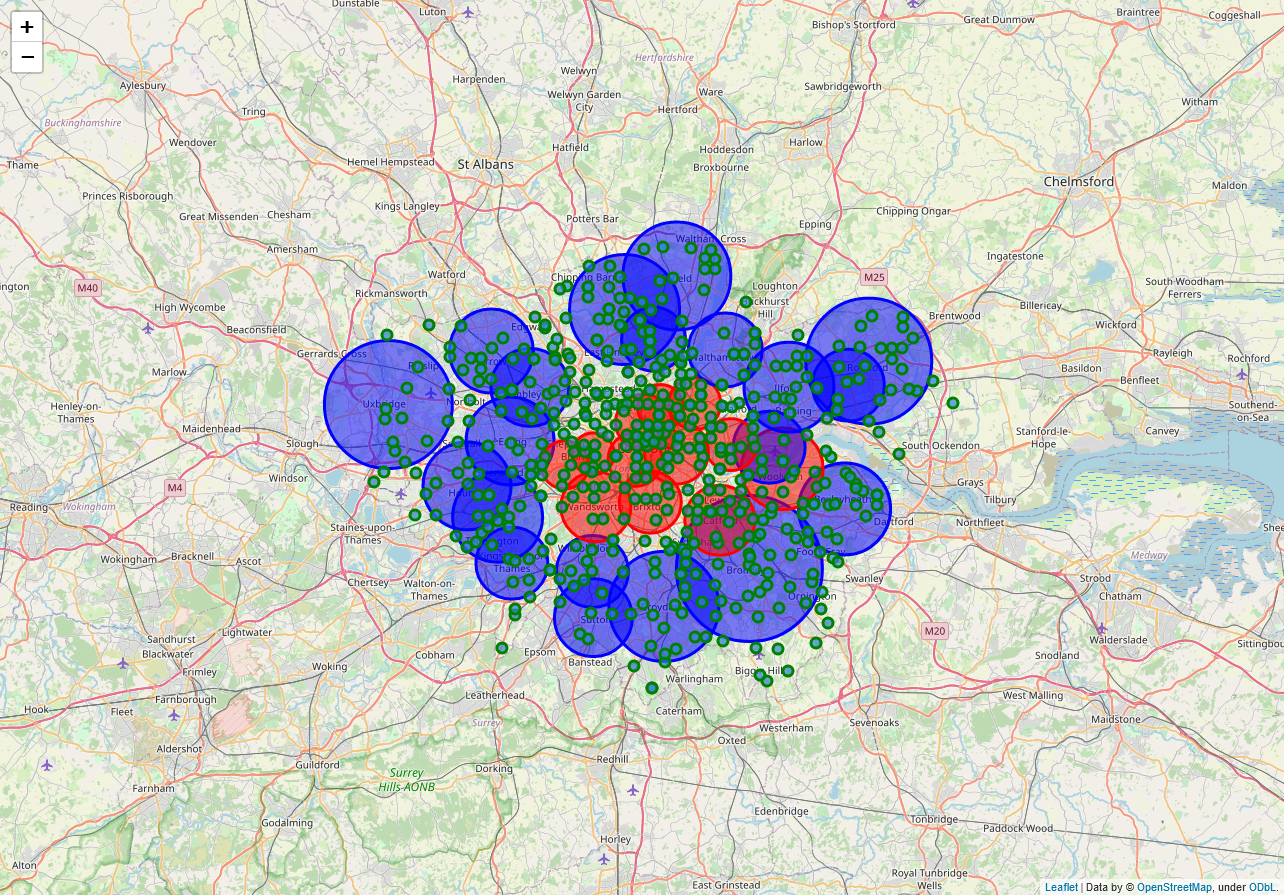
\includegraphics{01_borough_radius}\end{center}

            % \begin{tcolorbox}[breakable, size=fbox, boxrule=.5pt, pad at break*=1mm, opacityfill=0]
% % \prompt{Out}{outcolor}{32}{\boxspacing}
% \begin{Verbatim}[commandchars=\\\{\}]
% <folium.folium.Map at 0x221e76d8b80>
% \end{Verbatim}
% \end{tcolorbox}
        
    % \begin{tcolorbox}[breakable, size=fbox, boxrule=1pt, pad at break*=1mm,colback=cellbackground, colframe=cellborder]
% \prompt{In}{incolor}{33}{\boxspacing}
% \begin{Verbatim}[commandchars=\\\{\}]
% \PY{n}{save\PYZus{}map}\PY{p}{(}\PY{n}{map\PYZus{}london\PYZus{}borough\PYZus{}radius}\PY{p}{,} \PY{n}{file\PYZus{}name}\PY{o}{=}\PY{l+s+s1}{\PYZsq{}}\PY{l+s+s1}{01\PYZus{}borough\PYZus{}radius}\PY{l+s+s1}{\PYZsq{}}\PY{p}{)}
% \end{Verbatim}
% \end{tcolorbox}

    % \begin{Verbatim}[commandchars=\\\{\}]
% Map saved under '01\_borough\_radius.html' and '01\_borough\_radius.png'
    % \end{Verbatim}

    As we can see, circling the borough isn't the most appropriate way to
visualize neighborhoods. Let's try with a GeoJSON of the borough limits:

    % \begin{tcolorbox}[breakable, size=fbox, boxrule=1pt, pad at break*=1mm,colback=cellbackground, colframe=cellborder]
% \prompt{In}{incolor}{34}{\boxspacing}
% \begin{Verbatim}[commandchars=\\\{\}]
% \PY{n}{url\PYZus{}geolondon} \PY{o}{=} \PY{l+s+s2}{\PYZdq{}}\PY{l+s+s2}{https://skgrange.github.io/www/data/london\PYZus{}boroughs.json}\PY{l+s+s2}{\PYZdq{}}
% \PY{c+c1}{\PYZsh{}url\PYZus{}geoinner = \PYZdq{}https://skgrange.github.io/www/data/inner\PYZus{}london\PYZus{}polygons.json\PYZdq{}}

% \PY{n}{map\PYZus{}london\PYZus{}borough\PYZus{}geojson} \PY{o}{=} \PY{n}{folium}\PY{o}{.}\PY{n}{Map}\PY{p}{(}\PY{n}{location}\PY{o}{=}\PY{p}{[}\PY{n}{latitude}\PY{p}{,} \PY{n}{longitude}\PY{p}{]}\PY{p}{,} \PY{n}{tiles}\PY{o}{=}\PY{l+s+s1}{\PYZsq{}}\PY{l+s+s1}{OpenStreetMap}\PY{l+s+s1}{\PYZsq{}}\PY{p}{,} \PY{n}{zoom\PYZus{}start}\PY{o}{=}\PY{l+m+mi}{10}\PY{p}{)}

% \PY{c+c1}{\PYZsh{} Choropleth}
% \PY{n}{folium}\PY{o}{.}\PY{n}{Choropleth}\PY{p}{(}
    % \PY{n}{geo\PYZus{}data}\PY{o}{=}\PY{n}{url\PYZus{}geolondon}\PY{p}{,}
    % \PY{n}{data}\PY{o}{=}\PY{n}{borough\PYZus{}data}\PY{p}{,}
    % \PY{n}{columns}\PY{o}{=}\PY{p}{[}\PY{l+s+s1}{\PYZsq{}}\PY{l+s+s1}{Borough}\PY{l+s+s1}{\PYZsq{}}\PY{p}{,} \PY{l+s+s1}{\PYZsq{}}\PY{l+s+s1}{Inner}\PY{l+s+s1}{\PYZsq{}}\PY{p}{]}\PY{p}{,}
    % \PY{n}{key\PYZus{}on}\PY{o}{=}\PY{l+s+s1}{\PYZsq{}}\PY{l+s+s1}{feature.properties.name}\PY{l+s+s1}{\PYZsq{}}\PY{p}{,}
    % \PY{n}{fill\PYZus{}color}\PY{o}{=}\PY{l+s+s1}{\PYZsq{}}\PY{l+s+s1}{YlOrRd}\PY{l+s+s1}{\PYZsq{}}\PY{p}{,} 
    % \PY{n}{fill\PYZus{}opacity}\PY{o}{=}\PY{l+m+mf}{0.7}\PY{p}{,} 
    % \PY{n}{line\PYZus{}opacity}\PY{o}{=}\PY{l+m+mf}{0.2}\PY{p}{,}
    % \PY{n}{reset}\PY{o}{=}\PY{k+kc}{True}
% \PY{p}{)}\PY{o}{.}\PY{n}{add\PYZus{}to}\PY{p}{(}\PY{n}{map\PYZus{}london\PYZus{}borough\PYZus{}geojson}\PY{p}{)}

% \PY{c+c1}{\PYZsh{} Neighborhoods}
% \PY{k}{for} \PY{n}{lat}\PY{p}{,} \PY{n}{lng}\PY{p}{,} \PY{n}{borough}\PY{p}{,} \PY{n}{neighborhood} \PY{o+ow}{in} \PY{n+nb}{zip}\PY{p}{(}\PY{n}{neigh\PYZus{}data}\PY{p}{[}\PY{l+s+s1}{\PYZsq{}}\PY{l+s+s1}{Latitude}\PY{l+s+s1}{\PYZsq{}}\PY{p}{]}\PY{p}{,} \PY{n}{neigh\PYZus{}data}\PY{p}{[}\PY{l+s+s1}{\PYZsq{}}\PY{l+s+s1}{Longitude}\PY{l+s+s1}{\PYZsq{}}\PY{p}{]}\PY{p}{,} \PY{n}{neigh\PYZus{}data}\PY{p}{[}\PY{l+s+s1}{\PYZsq{}}\PY{l+s+s1}{Borough}\PY{l+s+s1}{\PYZsq{}}\PY{p}{]}\PY{p}{,} \PY{n}{neigh\PYZus{}data}\PY{p}{[}\PY{l+s+s1}{\PYZsq{}}\PY{l+s+s1}{Neighborhood}\PY{l+s+s1}{\PYZsq{}}\PY{p}{]}\PY{p}{)}\PY{p}{:}
    % \PY{n}{label} \PY{o}{=} \PY{l+s+s1}{\PYZsq{}}\PY{l+s+si}{\PYZob{}\PYZcb{}}\PY{l+s+s1}{, }\PY{l+s+si}{\PYZob{}\PYZcb{}}\PY{l+s+s1}{\PYZsq{}}\PY{o}{.}\PY{n}{format}\PY{p}{(}\PY{n}{neighborhood}\PY{p}{,} \PY{n}{borough}\PY{p}{)}
    % \PY{n}{label} \PY{o}{=} \PY{n}{folium}\PY{o}{.}\PY{n}{Popup}\PY{p}{(}\PY{n}{label}\PY{p}{,} \PY{n}{parse\PYZus{}html}\PY{o}{=}\PY{k+kc}{True}\PY{p}{)}
    % \PY{n}{folium}\PY{o}{.}\PY{n}{CircleMarker}\PY{p}{(}
        % \PY{p}{[}\PY{n}{lat}\PY{p}{,} \PY{n}{lng}\PY{p}{]}\PY{p}{,}
        % \PY{n}{radius}\PY{o}{=}\PY{l+m+mi}{5}\PY{p}{,}
        % \PY{n}{popup}\PY{o}{=}\PY{n}{label}\PY{p}{,}
        % \PY{n}{color}\PY{o}{=}\PY{l+s+s1}{\PYZsq{}}\PY{l+s+s1}{green}\PY{l+s+s1}{\PYZsq{}}\PY{p}{,}
        % \PY{n}{fill}\PY{o}{=}\PY{k+kc}{True}\PY{p}{,}
        % \PY{n}{fill\PYZus{}color}\PY{o}{=}\PY{l+s+s1}{\PYZsq{}}\PY{l+s+s1}{\PYZsh{}3186cc}\PY{l+s+s1}{\PYZsq{}}\PY{p}{,}
        % \PY{n}{fill\PYZus{}opacity}\PY{o}{=}\PY{l+m+mf}{0.7}\PY{p}{,}
        % \PY{n}{parse\PYZus{}html}\PY{o}{=}\PY{k+kc}{False}\PY{p}{)}\PY{o}{.}\PY{n}{add\PYZus{}to}\PY{p}{(}\PY{n}{map\PYZus{}london\PYZus{}borough\PYZus{}geojson}\PY{p}{)}

% \PY{c+c1}{\PYZsh{} Display map}
% \PY{n}{map\PYZus{}london\PYZus{}borough\PYZus{}geojson}
% \end{Verbatim}
% \end{tcolorbox}

\begin{center}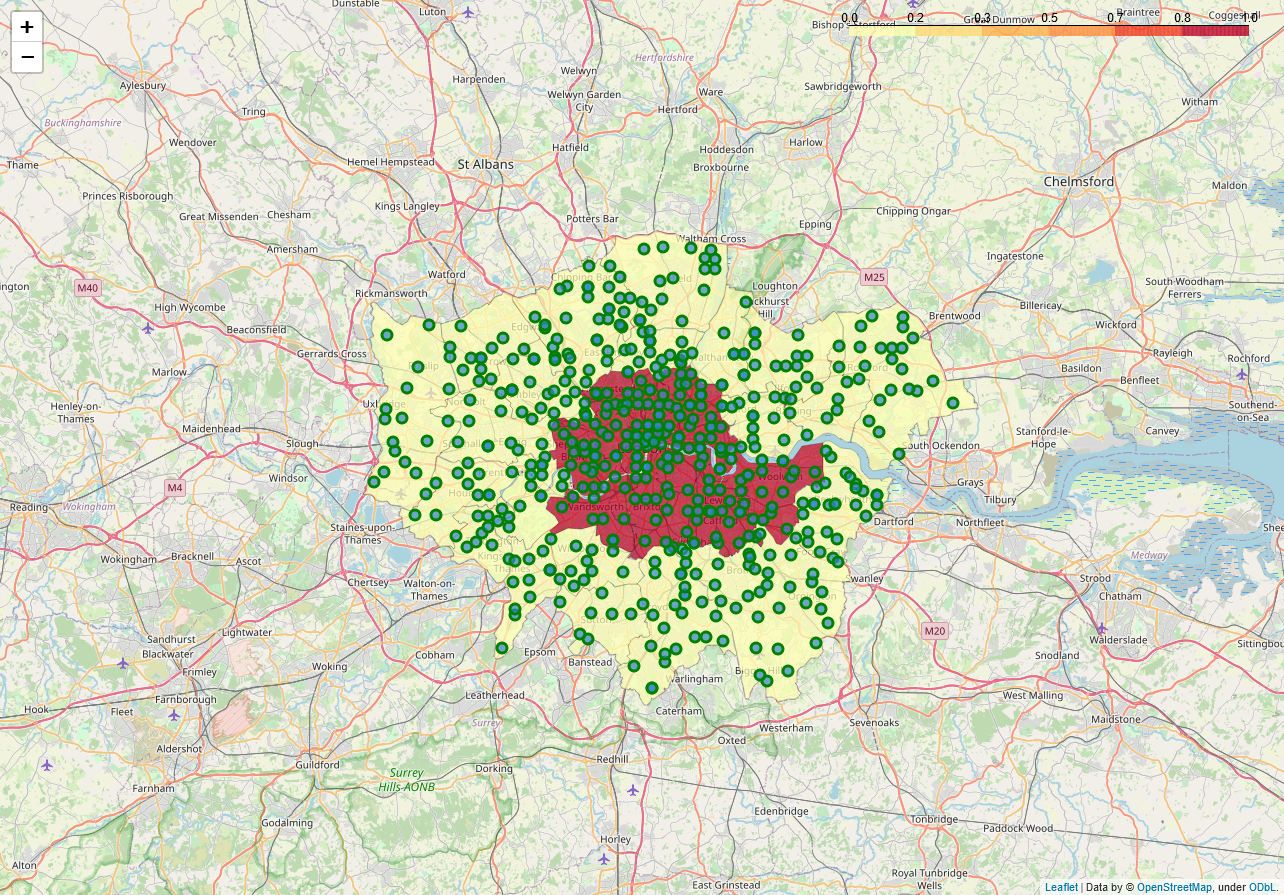
\includegraphics{02_borough_geojson}\end{center}

            % \begin{tcolorbox}[breakable, size=fbox, boxrule=.5pt, pad at break*=1mm, opacityfill=0]
% % \prompt{Out}{outcolor}{34}{\boxspacing}
% \begin{Verbatim}[commandchars=\\\{\}]
% <folium.folium.Map at 0x221e8dbf820>
% \end{Verbatim}
% \end{tcolorbox}
        
    % \begin{tcolorbox}[breakable, size=fbox, boxrule=1pt, pad at break*=1mm,colback=cellbackground, colframe=cellborder]
% \prompt{In}{incolor}{35}{\boxspacing}
% \begin{Verbatim}[commandchars=\\\{\}]
% \PY{n}{save\PYZus{}map}\PY{p}{(}\PY{n}{map\PYZus{}london\PYZus{}borough\PYZus{}geojson}\PY{p}{,} \PY{n}{file\PYZus{}name}\PY{o}{=}\PY{l+s+s1}{\PYZsq{}}\PY{l+s+s1}{02\PYZus{}borough\PYZus{}geojson}\PY{l+s+s1}{\PYZsq{}}\PY{p}{)}
% \end{Verbatim}
% \end{tcolorbox}

    % \begin{Verbatim}[commandchars=\\\{\}]
% Map saved under '02\_borough\_geojson.html' and '02\_borough\_geojson.png'
    % \end{Verbatim}

    It is already much clearer. And as we can see, the neighborhoods are
pretty spread appart.

London is a big city, and even the inner part of it is huge. Therefore,
it migth be best to create a sub-set of the data focusing on the City of
London borough. Let's first create a new dataset with a dummy column
indicating whether a neighborhood is part of the City of London or not:

    % \begin{tcolorbox}[breakable, size=fbox, boxrule=1pt, pad at break*=1mm,colback=cellbackground, colframe=cellborder]
% \prompt{In}{incolor}{36}{\boxspacing}
% \begin{Verbatim}[commandchars=\\\{\}]
% \PY{c+c1}{\PYZsh{} Join the two dataset}
% \PY{n}{inner\PYZus{}london\PYZus{}data} \PY{o}{=} \PY{n}{pd}\PY{o}{.}\PY{n}{merge}\PY{p}{(}\PY{n}{neigh\PYZus{}data}\PY{p}{,} \PY{n}{borough\PYZus{}data}\PY{p}{[}\PY{p}{[}\PY{l+s+s1}{\PYZsq{}}\PY{l+s+s1}{Borough}\PY{l+s+s1}{\PYZsq{}}\PY{p}{,}\PY{l+s+s1}{\PYZsq{}}\PY{l+s+s1}{Inner}\PY{l+s+s1}{\PYZsq{}}\PY{p}{]}\PY{p}{]}\PY{p}{,} \PY{n}{on}\PY{o}{=}\PY{l+s+s1}{\PYZsq{}}\PY{l+s+s1}{Borough}\PY{l+s+s1}{\PYZsq{}}\PY{p}{)}

% \PY{c+c1}{\PYZsh{} Drop rows that are not part of Inner London}
% \PY{n}{inner\PYZus{}london\PYZus{}data} \PY{o}{=} \PY{n}{inner\PYZus{}london\PYZus{}data}\PY{p}{[}\PY{n}{inner\PYZus{}london\PYZus{}data}\PY{p}{[}\PY{l+s+s1}{\PYZsq{}}\PY{l+s+s1}{Inner}\PY{l+s+s1}{\PYZsq{}}\PY{p}{]} \PY{o}{==} \PY{l+m+mi}{1}\PY{p}{]} \PY{o}{.}\PY{n}{reset\PYZus{}index}\PY{p}{(}\PY{n}{drop}\PY{o}{=}\PY{k+kc}{True}\PY{p}{)}
% \PY{n}{inner\PYZus{}london\PYZus{}data}\PY{o}{.}\PY{n}{drop}\PY{p}{(}\PY{n}{columns}\PY{o}{=}\PY{p}{[}\PY{l+s+s1}{\PYZsq{}}\PY{l+s+s1}{Inner}\PY{l+s+s1}{\PYZsq{}}\PY{p}{]}\PY{p}{,} \PY{n}{axis}\PY{o}{=}\PY{l+m+mi}{1}\PY{p}{,} \PY{n}{inplace}\PY{o}{=}\PY{k+kc}{True}\PY{p}{)}

% \PY{c+c1}{\PYZsh{} Add City column}
% \PY{n}{inner\PYZus{}london\PYZus{}data}\PY{p}{[}\PY{l+s+s1}{\PYZsq{}}\PY{l+s+s1}{City}\PY{l+s+s1}{\PYZsq{}}\PY{p}{]} \PY{o}{=} \PY{n}{pd}\PY{o}{.}\PY{n}{get\PYZus{}dummies}\PY{p}{(}\PY{n}{inner\PYZus{}london\PYZus{}data}\PY{p}{[}\PY{l+s+s1}{\PYZsq{}}\PY{l+s+s1}{Borough}\PY{l+s+s1}{\PYZsq{}}\PY{p}{]}\PY{o}{.}\PY{n}{replace}\PY{p}{(}\PY{p}{\PYZob{}}\PY{l+s+s1}{\PYZsq{}}\PY{l+s+s1}{\PYZca{}(?!City of London).*\PYZdl{}}\PY{l+s+s1}{\PYZsq{}}\PY{p}{:} \PY{k+kc}{None}\PY{p}{\PYZcb{}}\PY{p}{,} \PY{n}{regex}\PY{o}{=}\PY{k+kc}{True}\PY{p}{)}\PY{p}{)}

% \PY{c+c1}{\PYZsh{} Check results}
% \PY{n+nb}{print}\PY{p}{(}\PY{l+s+s2}{\PYZdq{}}\PY{l+s+s2}{Dataframe shape: }\PY{l+s+si}{\PYZob{}\PYZcb{}}\PY{l+s+s2}{\PYZdq{}}\PY{o}{.}\PY{n}{format}\PY{p}{(}\PY{n}{inner\PYZus{}london\PYZus{}data}\PY{o}{.}\PY{n}{shape}\PY{p}{)}\PY{p}{)}
% \PY{n+nb}{print}\PY{p}{(}\PY{l+s+s1}{\PYZsq{}}\PY{l+s+se}{\PYZbs{}n}\PY{l+s+s1}{\PYZsq{}}\PY{p}{)}
% \PY{n}{inner\PYZus{}london\PYZus{}data}\PY{o}{.}\PY{n}{head}\PY{p}{(}\PY{p}{)}
% \end{Verbatim}
% \end{tcolorbox}

% \resizebox{\textwidth}{!}{%
    \begin{tabular}{llllll}
    Dataframe shape: (180, 6)
    \\ \hline
    Borough & Neighborhood & Town & Latitude & Longitude & City
    \\ \hline
    City of London & Aldgate & London & 51.514885 & -0.078356 & 1
    \\
    City of London & Barbican & London & 51.519660 & -0.095466 & 1
    \\
    City of London & Blackfriars & London & 51.510767 & -0.101607 & 1
    \\
    City of London & Temple & London & 51.511828 & -0.111659 & 1
    \\
    Westminster & Aldwych & London & 51.512819 & -0.117388 & 0
    \end{tabular}
% }

    % \begin{Verbatim}[commandchars=\\\{\}]
% Dataframe shape: (180, 6)


    % \end{Verbatim}

            % \begin{tcolorbox}[breakable, size=fbox, boxrule=.5pt, pad at break*=1mm, opacityfill=0]
% % \prompt{Out}{outcolor}{36}{\boxspacing}
% \begin{Verbatim}[commandchars=\\\{\}]
          % Borough Neighborhood    Town   Latitude  Longitude  City
% 0  City of London      Aldgate  London  51.514885  -0.078356     1
% 1  City of London     Barbican  London  51.519660  -0.095466     1
% 2  City of London  Blackfriars  London  51.510767  -0.101607     1
% 3  City of London       Temple  London  51.511828  -0.111659     1
% 4     Westminster      Aldwych  London  51.512819  -0.117388     0
% \end{Verbatim}
% \end{tcolorbox}
        
    Let's also create another one containing only the neighborhoods for the
City of London:

    % \begin{tcolorbox}[breakable, size=fbox, boxrule=1pt, pad at break*=1mm,colback=cellbackground, colframe=cellborder]
% \prompt{In}{incolor}{37}{\boxspacing}
% \begin{Verbatim}[commandchars=\\\{\}]
% \PY{n}{london\PYZus{}city\PYZus{}data} \PY{o}{=} \PY{n}{neigh\PYZus{}data}\PY{p}{[}\PY{n}{neigh\PYZus{}data}\PY{p}{[}\PY{l+s+s1}{\PYZsq{}}\PY{l+s+s1}{Borough}\PY{l+s+s1}{\PYZsq{}}\PY{p}{]} \PY{o}{==} \PY{l+s+s1}{\PYZsq{}}\PY{l+s+s1}{City of London}\PY{l+s+s1}{\PYZsq{}}\PY{p}{]}\PY{o}{.}\PY{n}{reset\PYZus{}index}\PY{p}{(}\PY{n}{drop}\PY{o}{=}\PY{k+kc}{True}\PY{p}{)}

% \PY{c+c1}{\PYZsh{} Check results}
% \PY{n+nb}{print}\PY{p}{(}\PY{l+s+s2}{\PYZdq{}}\PY{l+s+s2}{Dataframe shape: }\PY{l+s+si}{\PYZob{}\PYZcb{}}\PY{l+s+s2}{\PYZdq{}}\PY{o}{.}\PY{n}{format}\PY{p}{(}\PY{n}{london\PYZus{}city\PYZus{}data}\PY{o}{.}\PY{n}{shape}\PY{p}{)}\PY{p}{)}
% \PY{n+nb}{print}\PY{p}{(}\PY{l+s+s1}{\PYZsq{}}\PY{l+s+se}{\PYZbs{}n}\PY{l+s+s1}{\PYZsq{}}\PY{p}{)}
% \PY{n}{london\PYZus{}city\PYZus{}data}\PY{o}{.}\PY{n}{head}\PY{p}{(}\PY{p}{)}
% \end{Verbatim}
% \end{tcolorbox}

% \resizebox{\textwidth}{!}{%
    \begin{tabular}{lllll}
    Dataframe shape: (4, 5)
    \\ \hline
    Borough & Neighborhood & Town & Latitude & Longitude
    \\ \hline
    City of London & Aldgate & London & 51.514885 & -0.078356
    \\
    City of London & Barbican & London & 51.519660 & -0.095466
    \\
    City of London & Blackfriars & London & 51.510767 & -0.101607
    \\
    City of London & Temple & London & 51.511828 & -0.111659
    \end{tabular}
% }

    % \begin{Verbatim}[commandchars=\\\{\}]
% Dataframe shape: (4, 5)


    % \end{Verbatim}

            % \begin{tcolorbox}[breakable, size=fbox, boxrule=.5pt, pad at break*=1mm, opacityfill=0]
% % \prompt{Out}{outcolor}{37}{\boxspacing}
% \begin{Verbatim}[commandchars=\\\{\}]
          % Borough Neighborhood    Town   Latitude  Longitude
% 0  City of London      Aldgate  London  51.514885  -0.078356
% 1  City of London     Barbican  London  51.519660  -0.095466
% 2  City of London  Blackfriars  London  51.510767  -0.101607
% 3  City of London       Temple  London  51.511828  -0.111659
% \end{Verbatim}
% \end{tcolorbox}
        
    Let's now compare the two dataset on a map, by plotting first every
neighborhoods in blue, then turning red the ones in London city:

    % \begin{tcolorbox}[breakable, size=fbox, boxrule=1pt, pad at break*=1mm,colback=cellbackground, colframe=cellborder]
% \prompt{In}{incolor}{38}{\boxspacing}
% \begin{Verbatim}[commandchars=\\\{\}]
% \PY{c+c1}{\PYZsh{} Create map of London using latitude and longitude values}
% \PY{n}{map\PYZus{}london\PYZus{}city\PYZus{}neigh} \PY{o}{=} \PY{n}{folium}\PY{o}{.}\PY{n}{Map}\PY{p}{(}\PY{n}{location}\PY{o}{=}\PY{p}{[}\PY{n}{latitude}\PY{p}{,} \PY{n}{longitude}\PY{p}{]}\PY{p}{,} \PY{n}{zoom\PYZus{}start}\PY{o}{=}\PY{l+m+mi}{11}\PY{p}{)}

% \PY{c+c1}{\PYZsh{} Add markers corresponding to the neighborhoods to the map}
% \PY{k}{for} \PY{n}{lat}\PY{p}{,} \PY{n}{lng}\PY{p}{,} \PY{n}{borough}\PY{p}{,} \PY{n}{neighborhood} \PY{o+ow}{in} \PY{n+nb}{zip}\PY{p}{(}\PY{n}{inner\PYZus{}london\PYZus{}data}\PY{p}{[}\PY{l+s+s1}{\PYZsq{}}\PY{l+s+s1}{Latitude}\PY{l+s+s1}{\PYZsq{}}\PY{p}{]}\PY{p}{,} \PY{n}{inner\PYZus{}london\PYZus{}data}\PY{p}{[}\PY{l+s+s1}{\PYZsq{}}\PY{l+s+s1}{Longitude}\PY{l+s+s1}{\PYZsq{}}\PY{p}{]}\PY{p}{,} \PY{n}{inner\PYZus{}london\PYZus{}data}\PY{p}{[}\PY{l+s+s1}{\PYZsq{}}\PY{l+s+s1}{Borough}\PY{l+s+s1}{\PYZsq{}}\PY{p}{]}\PY{p}{,} \PY{n}{inner\PYZus{}london\PYZus{}data}\PY{p}{[}\PY{l+s+s1}{\PYZsq{}}\PY{l+s+s1}{Neighborhood}\PY{l+s+s1}{\PYZsq{}}\PY{p}{]}\PY{p}{)}\PY{p}{:}
    % \PY{n}{label} \PY{o}{=} \PY{l+s+s1}{\PYZsq{}}\PY{l+s+si}{\PYZob{}\PYZcb{}}\PY{l+s+s1}{, }\PY{l+s+si}{\PYZob{}\PYZcb{}}\PY{l+s+s1}{\PYZsq{}}\PY{o}{.}\PY{n}{format}\PY{p}{(}\PY{n}{neighborhood}\PY{p}{,} \PY{n}{borough}\PY{p}{)}
    % \PY{n}{label} \PY{o}{=} \PY{n}{folium}\PY{o}{.}\PY{n}{Popup}\PY{p}{(}\PY{n}{label}\PY{p}{,} \PY{n}{parse\PYZus{}html}\PY{o}{=}\PY{k+kc}{True}\PY{p}{)}
    % \PY{n}{folium}\PY{o}{.}\PY{n}{CircleMarker}\PY{p}{(}
        % \PY{p}{[}\PY{n}{lat}\PY{p}{,} \PY{n}{lng}\PY{p}{]}\PY{p}{,}
        % \PY{n}{radius}\PY{o}{=}\PY{l+m+mi}{5}\PY{p}{,}
        % \PY{n}{popup}\PY{o}{=}\PY{n}{label}\PY{p}{,}
        % \PY{n}{color}\PY{o}{=}\PY{l+s+s1}{\PYZsq{}}\PY{l+s+s1}{blue}\PY{l+s+s1}{\PYZsq{}}\PY{p}{,}
        % \PY{n}{fill}\PY{o}{=}\PY{k+kc}{True}\PY{p}{,}
        % \PY{n}{fill\PYZus{}color}\PY{o}{=}\PY{l+s+s1}{\PYZsq{}}\PY{l+s+s1}{\PYZsh{}3186cc}\PY{l+s+s1}{\PYZsq{}}\PY{p}{,}
        % \PY{n}{fill\PYZus{}opacity}\PY{o}{=}\PY{l+m+mf}{0.7}\PY{p}{,}
        % \PY{n}{parse\PYZus{}html}\PY{o}{=}\PY{k+kc}{False}\PY{p}{)}\PY{o}{.}\PY{n}{add\PYZus{}to}\PY{p}{(}\PY{n}{map\PYZus{}london\PYZus{}city\PYZus{}neigh}\PY{p}{)}  

% \PY{c+c1}{\PYZsh{} Add markers corresponding to the neighborhoods to the map}
% \PY{k}{for} \PY{n}{lat}\PY{p}{,} \PY{n}{lng}\PY{p}{,} \PY{n}{borough}\PY{p}{,} \PY{n}{neighborhood} \PY{o+ow}{in} \PY{n+nb}{zip}\PY{p}{(}\PY{n}{london\PYZus{}city\PYZus{}data}\PY{p}{[}\PY{l+s+s1}{\PYZsq{}}\PY{l+s+s1}{Latitude}\PY{l+s+s1}{\PYZsq{}}\PY{p}{]}\PY{p}{,} \PY{n}{london\PYZus{}city\PYZus{}data}\PY{p}{[}\PY{l+s+s1}{\PYZsq{}}\PY{l+s+s1}{Longitude}\PY{l+s+s1}{\PYZsq{}}\PY{p}{]}\PY{p}{,} \PY{n}{london\PYZus{}city\PYZus{}data}\PY{p}{[}\PY{l+s+s1}{\PYZsq{}}\PY{l+s+s1}{Borough}\PY{l+s+s1}{\PYZsq{}}\PY{p}{]}\PY{p}{,} \PY{n}{london\PYZus{}city\PYZus{}data}\PY{p}{[}\PY{l+s+s1}{\PYZsq{}}\PY{l+s+s1}{Neighborhood}\PY{l+s+s1}{\PYZsq{}}\PY{p}{]}\PY{p}{)}\PY{p}{:}
    % \PY{n}{label} \PY{o}{=} \PY{l+s+s1}{\PYZsq{}}\PY{l+s+si}{\PYZob{}\PYZcb{}}\PY{l+s+s1}{, }\PY{l+s+si}{\PYZob{}\PYZcb{}}\PY{l+s+s1}{\PYZsq{}}\PY{o}{.}\PY{n}{format}\PY{p}{(}\PY{n}{neighborhood}\PY{p}{,} \PY{n}{borough}\PY{p}{)}
    % \PY{n}{label} \PY{o}{=} \PY{n}{folium}\PY{o}{.}\PY{n}{Popup}\PY{p}{(}\PY{n}{label}\PY{p}{,} \PY{n}{parse\PYZus{}html}\PY{o}{=}\PY{k+kc}{True}\PY{p}{)}
    % \PY{n}{folium}\PY{o}{.}\PY{n}{CircleMarker}\PY{p}{(}
        % \PY{p}{[}\PY{n}{lat}\PY{p}{,} \PY{n}{lng}\PY{p}{]}\PY{p}{,}
        % \PY{n}{radius}\PY{o}{=}\PY{l+m+mi}{5}\PY{p}{,}
        % \PY{n}{popup}\PY{o}{=}\PY{n}{label}\PY{p}{,}
        % \PY{n}{color}\PY{o}{=}\PY{l+s+s1}{\PYZsq{}}\PY{l+s+s1}{red}\PY{l+s+s1}{\PYZsq{}}\PY{p}{,}
        % \PY{n}{fill}\PY{o}{=}\PY{k+kc}{True}\PY{p}{,}
        % \PY{n}{fill\PYZus{}color}\PY{o}{=}\PY{l+s+s1}{\PYZsq{}}\PY{l+s+s1}{\PYZsh{}3186cc}\PY{l+s+s1}{\PYZsq{}}\PY{p}{,}
        % \PY{n}{fill\PYZus{}opacity}\PY{o}{=}\PY{l+m+mf}{0.7}\PY{p}{,}
        % \PY{n}{parse\PYZus{}html}\PY{o}{=}\PY{k+kc}{False}\PY{p}{)}\PY{o}{.}\PY{n}{add\PYZus{}to}\PY{p}{(}\PY{n}{map\PYZus{}london\PYZus{}city\PYZus{}neigh}\PY{p}{)}  

% \PY{c+c1}{\PYZsh{} Display the map}
% \PY{n}{map\PYZus{}london\PYZus{}city\PYZus{}neigh}
% \end{Verbatim}
% \end{tcolorbox}

\begin{center}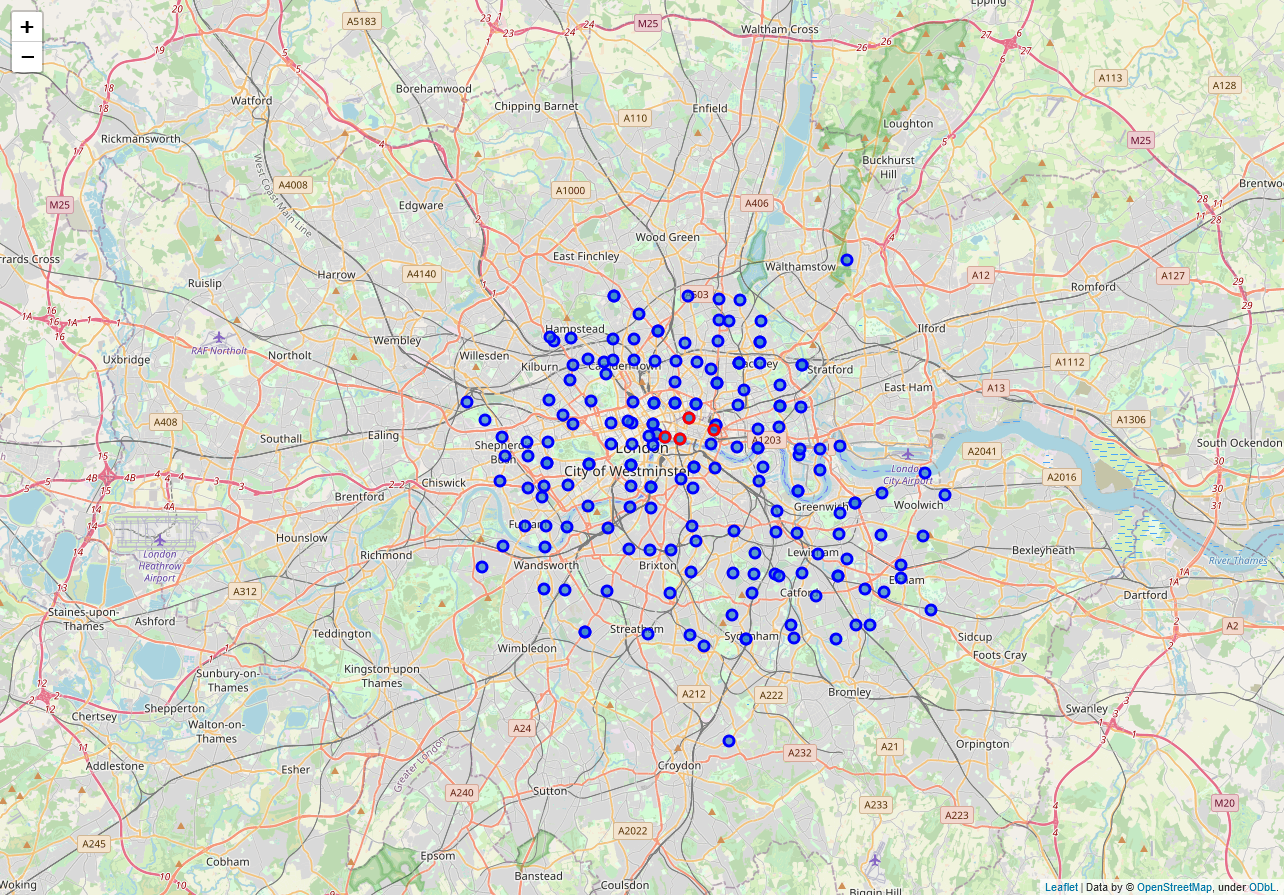
\includegraphics{03_londoncity_neighborhoods}\end{center}

            % \begin{tcolorbox}[breakable, size=fbox, boxrule=.5pt, pad at break*=1mm, opacityfill=0]
% % \prompt{Out}{outcolor}{38}{\boxspacing}
% \begin{Verbatim}[commandchars=\\\{\}]
% <folium.folium.Map at 0x221e8f474c0>
% \end{Verbatim}
% \end{tcolorbox}
        
    % \begin{tcolorbox}[breakable, size=fbox, boxrule=1pt, pad at break*=1mm,colback=cellbackground, colframe=cellborder]
% \prompt{In}{incolor}{39}{\boxspacing}
% \begin{Verbatim}[commandchars=\\\{\}]
% \PY{n}{save\PYZus{}map}\PY{p}{(}\PY{n}{map\PYZus{}london\PYZus{}city\PYZus{}neigh}\PY{p}{,} \PY{l+s+s1}{\PYZsq{}}\PY{l+s+s1}{03\PYZus{}londoncity\PYZus{}neighborhoods}\PY{l+s+s1}{\PYZsq{}}\PY{p}{)}
% \end{Verbatim}
% \end{tcolorbox}

    % \begin{Verbatim}[commandchars=\\\{\}]
% Map saved under '03\_londoncity\_neighborhoods.html' and
% '03\_londoncity\_neighborhoods.png'
    % \end{Verbatim}

    It is now clear that we need to focus more on areas around the City of
London. If we don't, our results will be too spread appart and won't be
relevant.

Let's have a quick look at how neighborhoods are spread around the City
of London, hereby in red:

    % \begin{tcolorbox}[breakable, size=fbox, boxrule=1pt, pad at break*=1mm,colback=cellbackground, colframe=cellborder]
% \prompt{In}{incolor}{40}{\boxspacing}
% \begin{Verbatim}[commandchars=\\\{\}]
% \PY{n}{city\PYZus{}latitude} \PY{o}{=} \PY{n}{borough\PYZus{}data}\PY{o}{.}\PY{n}{loc}\PY{p}{[}\PY{n}{borough\PYZus{}data}\PY{p}{[}\PY{l+s+s1}{\PYZsq{}}\PY{l+s+s1}{Borough}\PY{l+s+s1}{\PYZsq{}}\PY{p}{]} \PY{o}{==} \PY{l+s+s1}{\PYZsq{}}\PY{l+s+s1}{City of London}\PY{l+s+s1}{\PYZsq{}}\PY{p}{,} \PY{l+s+s1}{\PYZsq{}}\PY{l+s+s1}{Latitude}\PY{l+s+s1}{\PYZsq{}}\PY{p}{]}\PY{o}{.}\PY{n}{values}\PY{p}{[}\PY{l+m+mi}{0}\PY{p}{]}
% \PY{n}{city\PYZus{}longitude} \PY{o}{=} \PY{n}{borough\PYZus{}data}\PY{o}{.}\PY{n}{loc}\PY{p}{[}\PY{n}{borough\PYZus{}data}\PY{p}{[}\PY{l+s+s1}{\PYZsq{}}\PY{l+s+s1}{Borough}\PY{l+s+s1}{\PYZsq{}}\PY{p}{]} \PY{o}{==} \PY{l+s+s1}{\PYZsq{}}\PY{l+s+s1}{City of London}\PY{l+s+s1}{\PYZsq{}}\PY{p}{,} \PY{l+s+s1}{\PYZsq{}}\PY{l+s+s1}{Longitude}\PY{l+s+s1}{\PYZsq{}}\PY{p}{]}\PY{o}{.}\PY{n}{values}\PY{p}{[}\PY{l+m+mi}{0}\PY{p}{]}

% \PY{n}{map\PYZus{}london\PYZus{}city\PYZus{}boundaries} \PY{o}{=} \PY{n}{folium}\PY{o}{.}\PY{n}{Map}\PY{p}{(}\PY{n}{location}\PY{o}{=}\PY{p}{[}\PY{n}{city\PYZus{}latitude}\PY{p}{,} \PY{n}{city\PYZus{}longitude}\PY{p}{]}\PY{p}{,} \PY{n}{tiles}\PY{o}{=}\PY{l+s+s1}{\PYZsq{}}\PY{l+s+s1}{OpenStreetMap}\PY{l+s+s1}{\PYZsq{}}\PY{p}{,} \PY{n}{zoom\PYZus{}start}\PY{o}{=}\PY{l+m+mi}{13}\PY{p}{)}

% \PY{c+c1}{\PYZsh{} City center}
% \PY{n}{folium}\PY{o}{.}\PY{n}{Marker}\PY{p}{(}\PY{p}{[}\PY{n}{city\PYZus{}latitude}\PY{p}{,} \PY{n}{city\PYZus{}longitude}\PY{p}{]}\PY{p}{,} \PY{n}{icon}\PY{o}{=}\PY{n}{folium}\PY{o}{.}\PY{n}{Icon}\PY{p}{(}\PY{n}{color}\PY{o}{=}\PY{l+s+s1}{\PYZsq{}}\PY{l+s+s1}{red}\PY{l+s+s1}{\PYZsq{}}\PY{p}{,} \PY{n}{icon}\PY{o}{=}\PY{l+s+s1}{\PYZsq{}}\PY{l+s+s1}{info\PYZhy{}sign}\PY{l+s+s1}{\PYZsq{}}\PY{p}{)}\PY{p}{,} \PY{n}{popup}\PY{o}{=}\PY{l+s+s1}{\PYZsq{}}\PY{l+s+s1}{City Center}\PY{l+s+s1}{\PYZsq{}}\PY{p}{)}\PY{o}{.}\PY{n}{add\PYZus{}to}\PY{p}{(}\PY{n}{map\PYZus{}london\PYZus{}city\PYZus{}boundaries}\PY{p}{)}

% \PY{c+c1}{\PYZsh{} Choropleth}
% \PY{n}{folium}\PY{o}{.}\PY{n}{Choropleth}\PY{p}{(}
    % \PY{n}{geo\PYZus{}data}\PY{o}{=}\PY{n}{url\PYZus{}geolondon}\PY{p}{,}
    % \PY{n}{data}\PY{o}{=}\PY{n}{inner\PYZus{}london\PYZus{}data}\PY{p}{,}
    % \PY{n}{columns}\PY{o}{=}\PY{p}{[}\PY{l+s+s1}{\PYZsq{}}\PY{l+s+s1}{Borough}\PY{l+s+s1}{\PYZsq{}}\PY{p}{,} \PY{l+s+s1}{\PYZsq{}}\PY{l+s+s1}{City}\PY{l+s+s1}{\PYZsq{}}\PY{p}{]}\PY{p}{,}
    % \PY{n}{key\PYZus{}on}\PY{o}{=}\PY{l+s+s1}{\PYZsq{}}\PY{l+s+s1}{feature.properties.name}\PY{l+s+s1}{\PYZsq{}}\PY{p}{,}
    % \PY{n}{fill\PYZus{}color}\PY{o}{=}\PY{l+s+s1}{\PYZsq{}}\PY{l+s+s1}{YlOrRd}\PY{l+s+s1}{\PYZsq{}}\PY{p}{,} 
    % \PY{n}{fill\PYZus{}opacity}\PY{o}{=}\PY{l+m+mf}{0.7}\PY{p}{,} 
    % \PY{n}{line\PYZus{}opacity}\PY{o}{=}\PY{l+m+mf}{0.2}\PY{p}{,}
    % \PY{n}{reset}\PY{o}{=}\PY{k+kc}{True}
% \PY{p}{)}\PY{o}{.}\PY{n}{add\PYZus{}to}\PY{p}{(}\PY{n}{map\PYZus{}london\PYZus{}city\PYZus{}boundaries}\PY{p}{)}

% \PY{c+c1}{\PYZsh{} Neighborhoods}
% \PY{k}{for} \PY{n}{lat}\PY{p}{,} \PY{n}{lng}\PY{p}{,} \PY{n}{borough}\PY{p}{,} \PY{n}{neighborhood} \PY{o+ow}{in} \PY{n+nb}{zip}\PY{p}{(}\PY{n}{inner\PYZus{}london\PYZus{}data}\PY{p}{[}\PY{l+s+s1}{\PYZsq{}}\PY{l+s+s1}{Latitude}\PY{l+s+s1}{\PYZsq{}}\PY{p}{]}\PY{p}{,} \PY{n}{inner\PYZus{}london\PYZus{}data}\PY{p}{[}\PY{l+s+s1}{\PYZsq{}}\PY{l+s+s1}{Longitude}\PY{l+s+s1}{\PYZsq{}}\PY{p}{]}\PY{p}{,} \PY{n}{inner\PYZus{}london\PYZus{}data}\PY{p}{[}\PY{l+s+s1}{\PYZsq{}}\PY{l+s+s1}{Borough}\PY{l+s+s1}{\PYZsq{}}\PY{p}{]}\PY{p}{,} \PY{n}{inner\PYZus{}london\PYZus{}data}\PY{p}{[}\PY{l+s+s1}{\PYZsq{}}\PY{l+s+s1}{Neighborhood}\PY{l+s+s1}{\PYZsq{}}\PY{p}{]}\PY{p}{)}\PY{p}{:}
    % \PY{n}{label} \PY{o}{=} \PY{l+s+s1}{\PYZsq{}}\PY{l+s+si}{\PYZob{}\PYZcb{}}\PY{l+s+s1}{, }\PY{l+s+si}{\PYZob{}\PYZcb{}}\PY{l+s+s1}{\PYZsq{}}\PY{o}{.}\PY{n}{format}\PY{p}{(}\PY{n}{neighborhood}\PY{p}{,} \PY{n}{borough}\PY{p}{)}
    % \PY{n}{label} \PY{o}{=} \PY{n}{folium}\PY{o}{.}\PY{n}{Popup}\PY{p}{(}\PY{n}{label}\PY{p}{,} \PY{n}{parse\PYZus{}html}\PY{o}{=}\PY{k+kc}{True}\PY{p}{)}
    % \PY{n}{folium}\PY{o}{.}\PY{n}{CircleMarker}\PY{p}{(}
        % \PY{p}{[}\PY{n}{lat}\PY{p}{,} \PY{n}{lng}\PY{p}{]}\PY{p}{,}
        % \PY{n}{radius}\PY{o}{=}\PY{l+m+mi}{5}\PY{p}{,}
        % \PY{n}{popup}\PY{o}{=}\PY{n}{label}\PY{p}{,}
        % \PY{n}{color}\PY{o}{=}\PY{l+s+s1}{\PYZsq{}}\PY{l+s+s1}{green}\PY{l+s+s1}{\PYZsq{}}\PY{p}{,}
        % \PY{n}{fill}\PY{o}{=}\PY{k+kc}{True}\PY{p}{,}
        % \PY{n}{fill\PYZus{}color}\PY{o}{=}\PY{l+s+s1}{\PYZsq{}}\PY{l+s+s1}{\PYZsh{}3186cc}\PY{l+s+s1}{\PYZsq{}}\PY{p}{,}
        % \PY{n}{fill\PYZus{}opacity}\PY{o}{=}\PY{l+m+mf}{0.7}\PY{p}{,}
        % \PY{n}{parse\PYZus{}html}\PY{o}{=}\PY{k+kc}{False}\PY{p}{)}\PY{o}{.}\PY{n}{add\PYZus{}to}\PY{p}{(}\PY{n}{map\PYZus{}london\PYZus{}city\PYZus{}boundaries}\PY{p}{)}

% \PY{c+c1}{\PYZsh{} Display map}
% \PY{n}{map\PYZus{}london\PYZus{}city\PYZus{}boundaries}
% \end{Verbatim}
% \end{tcolorbox}

\begin{center}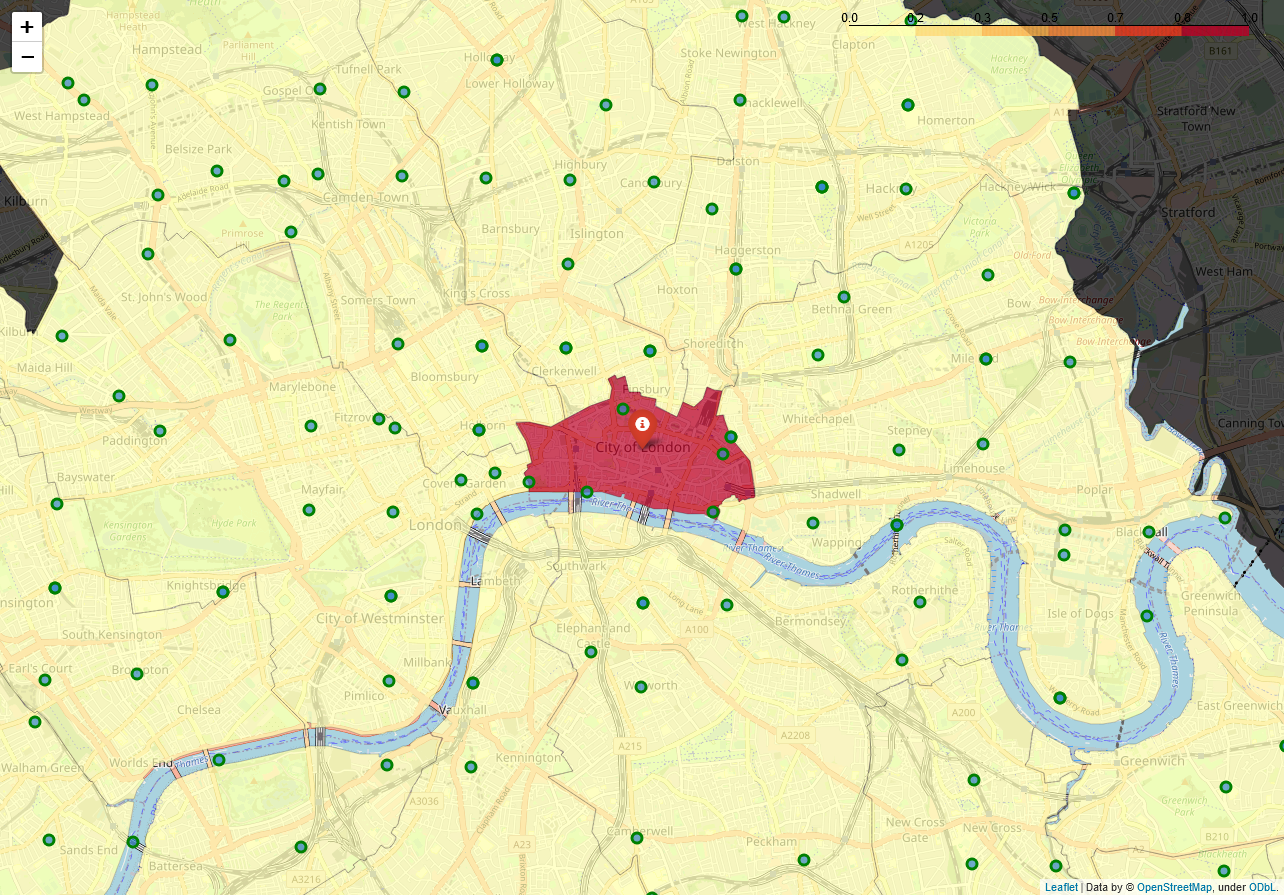
\includegraphics{04_londoncity_boundaries}\end{center}

            % \begin{tcolorbox}[breakable, size=fbox, boxrule=.5pt, pad at break*=1mm, opacityfill=0]
% % \prompt{Out}{outcolor}{40}{\boxspacing}
% \begin{Verbatim}[commandchars=\\\{\}]
% <folium.folium.Map at 0x221e9270d60>
% \end{Verbatim}
% \end{tcolorbox}
        
    % \begin{tcolorbox}[breakable, size=fbox, boxrule=1pt, pad at break*=1mm,colback=cellbackground, colframe=cellborder]
% \prompt{In}{incolor}{41}{\boxspacing}
% \begin{Verbatim}[commandchars=\\\{\}]
% \PY{n}{save\PYZus{}map}\PY{p}{(}\PY{n}{map\PYZus{}london\PYZus{}city\PYZus{}boundaries}\PY{p}{,} \PY{l+s+s1}{\PYZsq{}}\PY{l+s+s1}{04\PYZus{}londoncity\PYZus{}boundaries}\PY{l+s+s1}{\PYZsq{}}\PY{p}{)}
% \end{Verbatim}
% \end{tcolorbox}

    % \begin{Verbatim}[commandchars=\\\{\}]
% Map saved under '04\_londoncity\_boundaries.html' and
% '04\_londoncity\_boundaries.png'
    % \end{Verbatim}

    We can see that the City of London has few neighborhoods, but the other
boroughs contains some that are pretty close. Let's try another approach
and see whether it gives us better results at splitting the area.

We will create a grid of cells covering the City of London, with a
radius of 5km, therefore covering an approximate area of 10x10
kilometers around the City of London. For each grid, we will determine
the coordinates of its centroids, under the form of Latitude/Longitude,
but also X/Y carthesian coordinates. Those will be used to calculate
distances. Our neighborhoods will be defined as circular areas with a
radius of 250 meters, centers being 500m appart.

    Let us first define three functions to convert Latitude/Longitude into
Y/X coordinates, back and forth, and also compute the distance between
two points (X1, Y1) and (X2, Y2)

    % \begin{tcolorbox}[breakable, size=fbox, boxrule=1pt, pad at break*=1mm,colback=cellbackground, colframe=cellborder]
% \prompt{In}{incolor}{42}{\boxspacing}
% \begin{Verbatim}[commandchars=\\\{\}]
% \PY{k}{def} \PY{n+nf}{lonlat\PYZus{}to\PYZus{}xy}\PY{p}{(}\PY{n}{lon}\PY{p}{,} \PY{n}{lat}\PY{p}{)}\PY{p}{:}
    % \PY{n}{proj\PYZus{}xy} \PY{o}{=} \PY{n}{pyproj}\PY{o}{.}\PY{n}{Proj}\PY{p}{(}\PY{n}{proj}\PY{o}{=}\PY{l+s+s1}{\PYZsq{}}\PY{l+s+s1}{utm}\PY{l+s+s1}{\PYZsq{}}\PY{p}{,} \PY{n}{zone}\PY{o}{=}\PY{l+m+mi}{30}\PY{p}{,} \PY{n}{ellps}\PY{o}{=}\PY{l+s+s1}{\PYZsq{}}\PY{l+s+s1}{WGS84}\PY{l+s+s1}{\PYZsq{}}\PY{p}{,} \PY{n}{preserve\PYZus{}units}\PY{o}{=}\PY{k+kc}{False}\PY{p}{)}
    % \PY{n}{xy} \PY{o}{=} \PY{n}{proj\PYZus{}xy}\PY{p}{(}\PY{n}{lon}\PY{p}{,} \PY{n}{lat}\PY{p}{)}
    % \PY{k}{return} \PY{n}{xy}\PY{p}{[}\PY{l+m+mi}{0}\PY{p}{]}\PY{p}{,} \PY{n}{xy}\PY{p}{[}\PY{l+m+mi}{1}\PY{p}{]}

% \PY{k}{def} \PY{n+nf}{xy\PYZus{}to\PYZus{}lonlat}\PY{p}{(}\PY{n}{x}\PY{p}{,} \PY{n}{y}\PY{p}{)}\PY{p}{:}
    % \PY{n}{proj\PYZus{}latlon} \PY{o}{=} \PY{n}{pyproj}\PY{o}{.}\PY{n}{Proj}\PY{p}{(}\PY{n}{proj}\PY{o}{=}\PY{l+s+s1}{\PYZsq{}}\PY{l+s+s1}{utm}\PY{l+s+s1}{\PYZsq{}}\PY{p}{,} \PY{n}{zone}\PY{o}{=}\PY{l+m+mi}{30}\PY{p}{,} \PY{n}{ellps}\PY{o}{=}\PY{l+s+s1}{\PYZsq{}}\PY{l+s+s1}{WGS84}\PY{l+s+s1}{\PYZsq{}}\PY{p}{,} \PY{n}{preserve\PYZus{}units}\PY{o}{=}\PY{k+kc}{False}\PY{p}{)}
    % \PY{n}{lonlat} \PY{o}{=} \PY{n}{proj\PYZus{}latlon}\PY{p}{(}\PY{n}{x}\PY{p}{,} \PY{n}{y}\PY{p}{,} \PY{n}{inverse}\PY{o}{=}\PY{k+kc}{True}\PY{p}{)}
    % \PY{k}{return} \PY{n}{lonlat}\PY{p}{[}\PY{l+m+mi}{0}\PY{p}{]}\PY{p}{,} \PY{n}{lonlat}\PY{p}{[}\PY{l+m+mi}{1}\PY{p}{]}

% \PY{k}{def} \PY{n+nf}{calc\PYZus{}xy\PYZus{}distance}\PY{p}{(}\PY{n}{x1}\PY{p}{,} \PY{n}{y1}\PY{p}{,} \PY{n}{x2}\PY{p}{,} \PY{n}{y2}\PY{p}{)}\PY{p}{:}
    % \PY{n}{dx} \PY{o}{=} \PY{n}{x2} \PY{o}{\PYZhy{}} \PY{n}{x1}
    % \PY{n}{dy} \PY{o}{=} \PY{n}{y2} \PY{o}{\PYZhy{}} \PY{n}{y1}
    % \PY{k}{return} \PY{n}{math}\PY{o}{.}\PY{n}{sqrt}\PY{p}{(}\PY{n}{dx}\PY{o}{*}\PY{n}{dx} \PY{o}{+} \PY{n}{dy}\PY{o}{*}\PY{n}{dy}\PY{p}{)}

% \PY{n+nb}{print}\PY{p}{(}\PY{l+s+s1}{\PYZsq{}}\PY{l+s+s1}{Coordinate transformation check}\PY{l+s+s1}{\PYZsq{}}\PY{p}{)}
% \PY{n+nb}{print}\PY{p}{(}\PY{l+s+s1}{\PYZsq{}}\PY{l+s+s1}{\PYZhy{}\PYZhy{}\PYZhy{}\PYZhy{}\PYZhy{}\PYZhy{}\PYZhy{}\PYZhy{}\PYZhy{}\PYZhy{}\PYZhy{}\PYZhy{}\PYZhy{}\PYZhy{}\PYZhy{}\PYZhy{}\PYZhy{}\PYZhy{}\PYZhy{}\PYZhy{}\PYZhy{}\PYZhy{}\PYZhy{}\PYZhy{}\PYZhy{}\PYZhy{}\PYZhy{}\PYZhy{}\PYZhy{}\PYZhy{}\PYZhy{}}\PY{l+s+s1}{\PYZsq{}}\PY{p}{)}
% \PY{n+nb}{print}\PY{p}{(}\PY{l+s+s1}{\PYZsq{}}\PY{l+s+s1}{London center longitude=}\PY{l+s+si}{\PYZob{}\PYZcb{}}\PY{l+s+s1}{, latitude=}\PY{l+s+si}{\PYZob{}\PYZcb{}}\PY{l+s+s1}{\PYZsq{}}\PY{o}{.}\PY{n}{format}\PY{p}{(}\PY{n}{city\PYZus{}longitude}\PY{p}{,} \PY{n}{city\PYZus{}latitude}\PY{p}{)}\PY{p}{)}
% \PY{n}{x}\PY{p}{,} \PY{n}{y} \PY{o}{=} \PY{n}{lonlat\PYZus{}to\PYZus{}xy}\PY{p}{(}\PY{n}{city\PYZus{}longitude}\PY{p}{,} \PY{n}{city\PYZus{}latitude}\PY{p}{)}
% \PY{n+nb}{print}\PY{p}{(}\PY{l+s+s1}{\PYZsq{}}\PY{l+s+s1}{London center UTM X=}\PY{l+s+si}{\PYZob{}\PYZcb{}}\PY{l+s+s1}{, Y=}\PY{l+s+si}{\PYZob{}\PYZcb{}}\PY{l+s+s1}{\PYZsq{}}\PY{o}{.}\PY{n}{format}\PY{p}{(}\PY{n}{x}\PY{p}{,} \PY{n}{y}\PY{p}{)}\PY{p}{)}
% \PY{n}{lo}\PY{p}{,} \PY{n}{la} \PY{o}{=} \PY{n}{xy\PYZus{}to\PYZus{}lonlat}\PY{p}{(}\PY{n}{x}\PY{p}{,} \PY{n}{y}\PY{p}{)}
% \PY{n+nb}{print}\PY{p}{(}\PY{l+s+s1}{\PYZsq{}}\PY{l+s+s1}{London center longitude=}\PY{l+s+si}{\PYZob{}\PYZcb{}}\PY{l+s+s1}{, latitude=}\PY{l+s+si}{\PYZob{}\PYZcb{}}\PY{l+s+s1}{\PYZsq{}}\PY{o}{.}\PY{n}{format}\PY{p}{(}\PY{n}{lo}\PY{p}{,} \PY{n}{la}\PY{p}{)}\PY{p}{)}
% \end{Verbatim}
% \end{tcolorbox}

    \begin{Verbatim}[commandchars=\\\{\}]
Coordinate transformation check
-------------------------------
London center longitude=-0.0922, latitude=51.5155
London center UTM X=701750.4156930902, Y=5711161.921987954
London center longitude=-0.09219999999999916, latitude=51.51550000000001
    \end{Verbatim}

    Now let's generate a grid of areas around the center of the City of
London

Let's create a \textbf{hexagonal grid of cells}: we offset every other
row, and adjust vertical row spacing so that \textbf{every cell center
is equally distant from all it's neighbors}.

After that, we will store the results into a dataframe:

    % \begin{tcolorbox}[breakable, size=fbox, boxrule=1pt, pad at break*=1mm,colback=cellbackground, colframe=cellborder]
% \prompt{In}{incolor}{43}{\boxspacing}
% \begin{Verbatim}[commandchars=\\\{\}]
% \PY{n}{city\PYZus{}center\PYZus{}x}\PY{p}{,} \PY{n}{city\PYZus{}center\PYZus{}y} \PY{o}{=} \PY{n}{lonlat\PYZus{}to\PYZus{}xy}\PY{p}{(}\PY{n}{city\PYZus{}longitude}\PY{p}{,} \PY{n}{city\PYZus{}latitude}\PY{p}{)} \PY{c+c1}{\PYZsh{} City center in Cartesian coordinates}

% \PY{n}{k} \PY{o}{=} \PY{n}{math}\PY{o}{.}\PY{n}{sqrt}\PY{p}{(}\PY{l+m+mi}{3}\PY{p}{)} \PY{o}{/} \PY{l+m+mi}{2} \PY{c+c1}{\PYZsh{} Vertical offset for hexagonal grid cells}
% \PY{n}{x\PYZus{}min} \PY{o}{=} \PY{n}{city\PYZus{}center\PYZus{}x} \PY{o}{\PYZhy{}} \PY{l+m+mi}{5000}
% \PY{n}{x\PYZus{}step} \PY{o}{=} \PY{l+m+mi}{500}
% \PY{n}{y\PYZus{}min} \PY{o}{=} \PY{n}{city\PYZus{}center\PYZus{}y} \PY{o}{\PYZhy{}} \PY{l+m+mi}{5000} \PY{o}{\PYZhy{}} \PY{p}{(}\PY{n+nb}{int}\PY{p}{(}\PY{l+m+mi}{21}\PY{o}{/}\PY{n}{k}\PY{p}{)}\PY{o}{*}\PY{n}{k}\PY{o}{*}\PY{l+m+mi}{500} \PY{o}{\PYZhy{}} \PY{l+m+mi}{10000}\PY{p}{)}\PY{o}{/}\PY{l+m+mi}{2}
% \PY{n}{y\PYZus{}step} \PY{o}{=} \PY{l+m+mi}{500} \PY{o}{*} \PY{n}{k} 

% \PY{n}{lat\PYZus{}all} \PY{o}{=} \PY{p}{[}\PY{p}{]}
% \PY{n}{long\PYZus{}all} \PY{o}{=} \PY{p}{[}\PY{p}{]}
% \PY{n}{dist\PYZus{}center\PYZus{}all} \PY{o}{=} \PY{p}{[}\PY{p}{]}
% \PY{n}{xs\PYZus{}all} \PY{o}{=} \PY{p}{[}\PY{p}{]}
% \PY{n}{ys\PYZus{}all} \PY{o}{=} \PY{p}{[}\PY{p}{]}
% \PY{k}{for} \PY{n}{i} \PY{o+ow}{in} \PY{n+nb}{range}\PY{p}{(}\PY{l+m+mi}{0}\PY{p}{,} \PY{n+nb}{int}\PY{p}{(}\PY{l+m+mi}{21}\PY{o}{/}\PY{n}{k}\PY{p}{)}\PY{p}{)}\PY{p}{:}
    % \PY{n}{y} \PY{o}{=} \PY{n}{y\PYZus{}min} \PY{o}{+} \PY{n}{i} \PY{o}{*} \PY{n}{y\PYZus{}step}
    % \PY{n}{x\PYZus{}offset} \PY{o}{=} \PY{l+m+mi}{250} \PY{k}{if} \PY{n}{i}\PY{o}{\PYZpc{}}\PY{k}{2}==0 else 0
    % \PY{k}{for} \PY{n}{j} \PY{o+ow}{in} \PY{n+nb}{range}\PY{p}{(}\PY{l+m+mi}{0}\PY{p}{,} \PY{l+m+mi}{21}\PY{p}{)}\PY{p}{:}
        % \PY{n}{x} \PY{o}{=} \PY{n}{x\PYZus{}min} \PY{o}{+} \PY{n}{j} \PY{o}{*} \PY{n}{x\PYZus{}step} \PY{o}{+} \PY{n}{x\PYZus{}offset}
        % \PY{n}{dist\PYZus{}center} \PY{o}{=} \PY{n}{calc\PYZus{}xy\PYZus{}distance}\PY{p}{(}\PY{n}{city\PYZus{}center\PYZus{}x}\PY{p}{,} \PY{n}{city\PYZus{}center\PYZus{}y}\PY{p}{,} \PY{n}{x}\PY{p}{,} \PY{n}{y}\PY{p}{)}
        % \PY{k}{if} \PY{p}{(}\PY{n}{dist\PYZus{}center} \PY{o}{\PYZlt{}}\PY{o}{=} \PY{l+m+mi}{5001}\PY{p}{)}\PY{p}{:}
            % \PY{n}{lon}\PY{p}{,} \PY{n}{lat} \PY{o}{=} \PY{n}{xy\PYZus{}to\PYZus{}lonlat}\PY{p}{(}\PY{n}{x}\PY{p}{,} \PY{n}{y}\PY{p}{)}
            % \PY{n}{lat\PYZus{}all}\PY{o}{.}\PY{n}{append}\PY{p}{(}\PY{n}{lat}\PY{p}{)}
            % \PY{n}{long\PYZus{}all}\PY{o}{.}\PY{n}{append}\PY{p}{(}\PY{n}{lon}\PY{p}{)}
            % \PY{n}{dist\PYZus{}center\PYZus{}all}\PY{o}{.}\PY{n}{append}\PY{p}{(}\PY{n}{dist\PYZus{}center}\PY{p}{)}
            % \PY{n}{xs\PYZus{}all}\PY{o}{.}\PY{n}{append}\PY{p}{(}\PY{n}{x}\PY{p}{)}
            % \PY{n}{ys\PYZus{}all}\PY{o}{.}\PY{n}{append}\PY{p}{(}\PY{n}{y}\PY{p}{)}

% \PY{n+nb}{print}\PY{p}{(}\PY{n+nb}{len}\PY{p}{(}\PY{n}{lat\PYZus{}all}\PY{p}{)}\PY{p}{,} \PY{l+s+s1}{\PYZsq{}}\PY{l+s+s1}{candidate neighborhood centers generated.}\PY{l+s+s1}{\PYZsq{}}\PY{p}{)}
% \end{Verbatim}
% \end{tcolorbox}

\resizebox{\textwidth}{!}{%
    \begin{tabular}{lllll}
    364 candidate neighborhood centers generated.
    \\ \hline
    Latitude & Longitude & Distance from Center & X & Y
    \\ \hline
    51.473259 & -0.116492 & 4993.746089 & 700250.415693 & 5.706399e+06
    \\
    51.473082 & -0.109302 & 4866.980583 & 700750.415693 & 5.706399e+06
    \\
    51.472904 & -0.102112 & 4789.311015 & 701250.415693 & 5.706399e+06
    \\
    51.472726 & -0.094922 & 4763.139721 & 701750.415693 & 5.706399e+06
    \\
    51.472548 & -0.087733 & 4789.311015 & 702250.415693 & 5.706399e+06
    \end{tabular}
}

    % \begin{Verbatim}[commandchars=\\\{\}]
% 364 candidate neighborhood centers generated.
    % \end{Verbatim}

    % \begin{tcolorbox}[breakable, size=fbox, boxrule=1pt, pad at break*=1mm,colback=cellbackground, colframe=cellborder]
% \prompt{In}{incolor}{44}{\boxspacing}
% \begin{Verbatim}[commandchars=\\\{\}]
% \PY{n}{hexa\PYZus{}all} \PY{o}{=} \PY{n}{pd}\PY{o}{.}\PY{n}{DataFrame}\PY{p}{(}\PY{n+nb}{list}\PY{p}{(}\PY{n+nb}{zip}\PY{p}{(}\PY{n}{lat\PYZus{}all}\PY{p}{,} \PY{n}{long\PYZus{}all}\PY{p}{,} \PY{n}{dist\PYZus{}center\PYZus{}all}\PY{p}{,} \PY{n}{xs\PYZus{}all}\PY{p}{,} \PY{n}{ys\PYZus{}all}\PY{p}{)}\PY{p}{)}\PY{p}{,}
                        % \PY{n}{columns}\PY{o}{=}\PY{p}{[}\PY{l+s+s1}{\PYZsq{}}\PY{l+s+s1}{Latitude}\PY{l+s+s1}{\PYZsq{}}\PY{p}{,}\PY{l+s+s1}{\PYZsq{}}\PY{l+s+s1}{Longitude}\PY{l+s+s1}{\PYZsq{}}\PY{p}{,}\PY{l+s+s1}{\PYZsq{}}\PY{l+s+s1}{Distance from Center}\PY{l+s+s1}{\PYZsq{}}\PY{p}{,}\PY{l+s+s1}{\PYZsq{}}\PY{l+s+s1}{X}\PY{l+s+s1}{\PYZsq{}}\PY{p}{,}\PY{l+s+s1}{\PYZsq{}}\PY{l+s+s1}{Y}\PY{l+s+s1}{\PYZsq{}}\PY{p}{]}\PY{p}{)}
% \PY{n}{hexa\PYZus{}all}\PY{o}{.}\PY{n}{head}\PY{p}{(}\PY{p}{)}
% \end{Verbatim}
% \end{tcolorbox}

            % \begin{tcolorbox}[breakable, size=fbox, boxrule=.5pt, pad at break*=1mm, opacityfill=0]
% % \prompt{Out}{outcolor}{44}{\boxspacing}
% \begin{Verbatim}[commandchars=\\\{\}]
    % Latitude  Longitude  Distance from Center              X             Y
% 0  51.473259  -0.116492           4993.746089  700250.415693  5.706399e+06
% 1  51.473082  -0.109302           4866.980583  700750.415693  5.706399e+06
% 2  51.472904  -0.102112           4789.311015  701250.415693  5.706399e+06
% 3  51.472726  -0.094922           4763.139721  701750.415693  5.706399e+06
% 4  51.472548  -0.087733           4789.311015  702250.415693  5.706399e+06
% \end{Verbatim}
% \end{tcolorbox}
        
    Let's visualize the data we have so far, by plotting our areas around
the center of the city:

    % \begin{tcolorbox}[breakable, size=fbox, boxrule=1pt, pad at break*=1mm,colback=cellbackground, colframe=cellborder]
% \prompt{In}{incolor}{45}{\boxspacing}
% \begin{Verbatim}[commandchars=\\\{\}]
% \PY{n}{map\PYZus{}hexa\PYZus{}all} \PY{o}{=} \PY{n}{folium}\PY{o}{.}\PY{n}{Map}\PY{p}{(}\PY{n}{location}\PY{o}{=}\PY{p}{[}\PY{n}{city\PYZus{}latitude}\PY{p}{,} \PY{n}{city\PYZus{}longitude}\PY{p}{]}\PY{p}{,} \PY{n}{zoom\PYZus{}start}\PY{o}{=}\PY{l+m+mi}{13}\PY{p}{)}

% \PY{c+c1}{\PYZsh{} City center}
% \PY{n}{folium}\PY{o}{.}\PY{n}{Marker}\PY{p}{(}\PY{p}{[}\PY{n}{city\PYZus{}latitude}\PY{p}{,} \PY{n}{city\PYZus{}longitude}\PY{p}{]}\PY{p}{,} \PY{n}{icon}\PY{o}{=}\PY{n}{folium}\PY{o}{.}\PY{n}{Icon}\PY{p}{(}\PY{n}{color}\PY{o}{=}\PY{l+s+s1}{\PYZsq{}}\PY{l+s+s1}{red}\PY{l+s+s1}{\PYZsq{}}\PY{p}{,} \PY{n}{icon}\PY{o}{=}\PY{l+s+s1}{\PYZsq{}}\PY{l+s+s1}{info\PYZhy{}sign}\PY{l+s+s1}{\PYZsq{}}\PY{p}{)}\PY{p}{,} \PY{n}{popup}\PY{o}{=}\PY{l+s+s1}{\PYZsq{}}\PY{l+s+s1}{City Center}\PY{l+s+s1}{\PYZsq{}}\PY{p}{)}\PY{o}{.}\PY{n}{add\PYZus{}to}\PY{p}{(}\PY{n}{map\PYZus{}hexa\PYZus{}all}\PY{p}{)}

% \PY{c+c1}{\PYZsh{} Areas}
% \PY{k}{for} \PY{n}{lat}\PY{p}{,} \PY{n}{lon} \PY{o+ow}{in} \PY{n+nb}{zip}\PY{p}{(}\PY{n}{lat\PYZus{}all}\PY{p}{,} \PY{n}{long\PYZus{}all}\PY{p}{)}\PY{p}{:}
    % \PY{c+c1}{\PYZsh{}folium.CircleMarker([lat, lon], radius=2, color=\PYZsq{}blue\PYZsq{}, fill=True, fill\PYZus{}color=\PYZsq{}blue\PYZsq{}, fill\PYZus{}opacity=1).add\PYZus{}to(map\PYZus{}berlin) }
    % \PY{n}{folium}\PY{o}{.}\PY{n}{Circle}\PY{p}{(}\PY{p}{[}\PY{n}{lat}\PY{p}{,} \PY{n}{lon}\PY{p}{]}\PY{p}{,} \PY{n}{radius}\PY{o}{=}\PY{l+m+mi}{250}\PY{p}{,} \PY{n}{color}\PY{o}{=}\PY{l+s+s1}{\PYZsq{}}\PY{l+s+s1}{blue}\PY{l+s+s1}{\PYZsq{}}\PY{p}{,} \PY{n}{fill}\PY{o}{=}\PY{k+kc}{False}\PY{p}{)}\PY{o}{.}\PY{n}{add\PYZus{}to}\PY{p}{(}\PY{n}{map\PYZus{}hexa\PYZus{}all}\PY{p}{)}
    % \PY{c+c1}{\PYZsh{}folium.Marker([lat, lon]).add\PYZus{}to(map\PYZus{}berlin)}

% \PY{c+c1}{\PYZsh{} Display map}
% \PY{n}{map\PYZus{}hexa\PYZus{}all}
% \end{Verbatim}
% \end{tcolorbox}

\begin{center}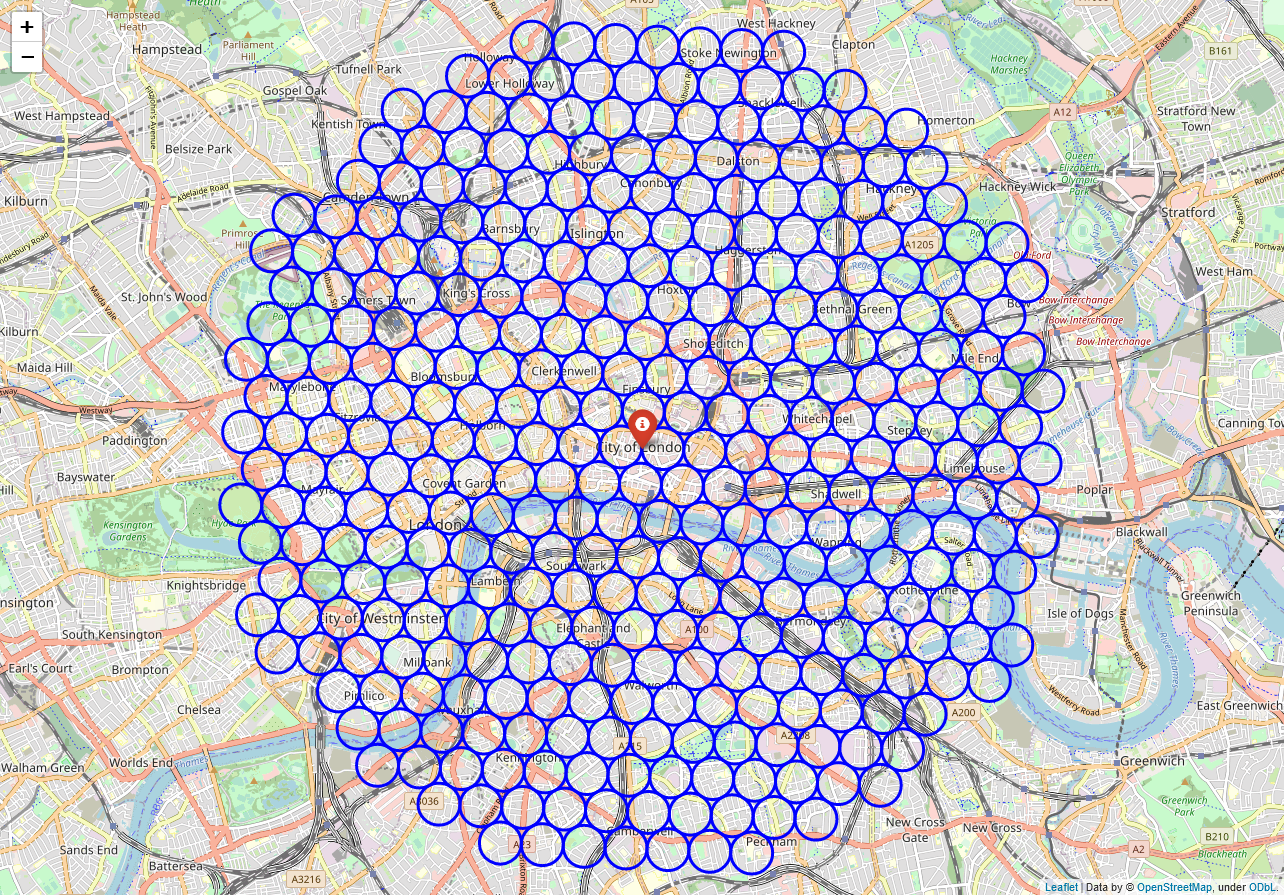
\includegraphics{05_hexa_areas_all}\end{center}

            % \begin{tcolorbox}[breakable, size=fbox, boxrule=.5pt, pad at break*=1mm, opacityfill=0]
% % \prompt{Out}{outcolor}{45}{\boxspacing}
% \begin{Verbatim}[commandchars=\\\{\}]
% <folium.folium.Map at 0x221e9e013a0>
% \end{Verbatim}
% \end{tcolorbox}
        
    % \begin{tcolorbox}[breakable, size=fbox, boxrule=1pt, pad at break*=1mm,colback=cellbackground, colframe=cellborder]
% \prompt{In}{incolor}{46}{\boxspacing}
% \begin{Verbatim}[commandchars=\\\{\}]
% \PY{n}{save\PYZus{}map}\PY{p}{(}\PY{n}{map\PYZus{}hexa\PYZus{}all}\PY{p}{,} \PY{l+s+s1}{\PYZsq{}}\PY{l+s+s1}{05\PYZus{}hexa\PYZus{}areas\PYZus{}all}\PY{l+s+s1}{\PYZsq{}}\PY{p}{)}
% \end{Verbatim}
% \end{tcolorbox}

    % \begin{Verbatim}[commandchars=\\\{\}]
% Map saved under '05\_hexa\_areas\_all.html' and '05\_hexa\_areas\_all.png'
    % \end{Verbatim}

    Now we can already see one problem with our areas: the River Thames.
Indeed, restaurants in the middle of the river would'nt be practical.

Let's retrieve the River Thames coordinates using a GeoJSON, then list
all areas within it, and storing them into a dataframe:

    % \begin{tcolorbox}[breakable, size=fbox, boxrule=1pt, pad at break*=1mm,colback=cellbackground, colframe=cellborder]
% \prompt{In}{incolor}{47}{\boxspacing}
% \begin{Verbatim}[commandchars=\\\{\}]
% \PY{c+c1}{\PYZsh{} load GeoJSON file containing sectors}
% \PY{c+c1}{\PYZsh{} https://jburnford.carto.com/tables/thames/public}
% \PY{k}{with} \PY{n+nb}{open}\PY{p}{(}\PY{l+s+s1}{\PYZsq{}}\PY{l+s+s1}{thames.geojson}\PY{l+s+s1}{\PYZsq{}}\PY{p}{)} \PY{k}{as} \PY{n}{f}\PY{p}{:}
    % \PY{n}{thames} \PY{o}{=} \PY{n}{json}\PY{o}{.}\PY{n}{load}\PY{p}{(}\PY{n}{f}\PY{p}{)}

% \PY{n}{lat\PYZus{}bad} \PY{o}{=} \PY{p}{[}\PY{p}{]}
% \PY{n}{long\PYZus{}bad} \PY{o}{=} \PY{p}{[}\PY{p}{]}
% \PY{n}{dist\PYZus{}center\PYZus{}bad} \PY{o}{=} \PY{p}{[}\PY{p}{]}
% \PY{n}{xs\PYZus{}bad} \PY{o}{=} \PY{p}{[}\PY{p}{]}
% \PY{n}{ys\PYZus{}bad} \PY{o}{=} \PY{p}{[}\PY{p}{]}

% \PY{c+c1}{\PYZsh{}print(lat\PYZus{}bis, long\PYZus{}bis)}

% \PY{k}{for} \PY{n}{lat}\PY{p}{,} \PY{n}{long}\PY{p}{,} \PY{n}{dist}\PY{p}{,} \PY{n}{x}\PY{p}{,} \PY{n}{y} \PY{o+ow}{in} \PY{n+nb}{zip}\PY{p}{(}\PY{n}{lat\PYZus{}all}\PY{p}{,} \PY{n}{long\PYZus{}all}\PY{p}{,} \PY{n}{dist\PYZus{}center\PYZus{}all}\PY{p}{,} \PY{n}{xs\PYZus{}all}\PY{p}{,} \PY{n}{ys\PYZus{}all}\PY{p}{)}\PY{p}{:}
    % \PY{n}{point} \PY{o}{=} \PY{n}{Point}\PY{p}{(}\PY{n}{long}\PY{p}{,} \PY{n}{lat}\PY{p}{)}
    % \PY{c+c1}{\PYZsh{} River Thames}
    % \PY{k}{for} \PY{n}{feature} \PY{o+ow}{in} \PY{n}{thames}\PY{p}{[}\PY{l+s+s1}{\PYZsq{}}\PY{l+s+s1}{features}\PY{l+s+s1}{\PYZsq{}}\PY{p}{]}\PY{p}{:}
        % \PY{n}{polygon} \PY{o}{=} \PY{n}{shape}\PY{p}{(}\PY{n}{feature}\PY{p}{[}\PY{l+s+s1}{\PYZsq{}}\PY{l+s+s1}{geometry}\PY{l+s+s1}{\PYZsq{}}\PY{p}{]}\PY{p}{)}
        % \PY{k}{if} \PY{n}{polygon}\PY{o}{.}\PY{n}{contains}\PY{p}{(}\PY{n}{point}\PY{p}{)}\PY{p}{:}
            % \PY{n}{lat\PYZus{}bad}\PY{o}{.}\PY{n}{append}\PY{p}{(}\PY{n}{lat}\PY{p}{)}
            % \PY{n}{long\PYZus{}bad}\PY{o}{.}\PY{n}{append}\PY{p}{(}\PY{n}{long}\PY{p}{)}
            % \PY{n}{dist\PYZus{}center\PYZus{}bad}\PY{o}{.}\PY{n}{append}\PY{p}{(}\PY{n}{dist}\PY{p}{)}
            % \PY{n}{xs\PYZus{}bad}\PY{o}{.}\PY{n}{append}\PY{p}{(}\PY{n}{x}\PY{p}{)}
            % \PY{n}{ys\PYZus{}bad}\PY{o}{.}\PY{n}{append}\PY{p}{(}\PY{n}{y}\PY{p}{)}
            % \PY{k}{break}

% \PY{n+nb}{print}\PY{p}{(}\PY{l+s+s1}{\PYZsq{}}\PY{l+s+si}{\PYZob{}\PYZcb{}}\PY{l+s+s1}{ coordinates to be removed out of }\PY{l+s+si}{\PYZob{}\PYZcb{}}\PY{l+s+s1}{\PYZsq{}}\PY{o}{.}\PY{n}{format}\PY{p}{(}\PY{n+nb}{len}\PY{p}{(}\PY{n}{lat\PYZus{}bad}\PY{p}{)}\PY{p}{,} \PY{n+nb}{len}\PY{p}{(}\PY{n}{lat\PYZus{}all}\PY{p}{)}\PY{p}{)}\PY{p}{)}
% \end{Verbatim}
% \end{tcolorbox}

\resizebox{\textwidth}{!}{%
    \begin{tabular}{lllll}
    14 coordinates to be removed out of 364
    \\ \hline
    Latitude & Longitude & Distance from Center & X & Y
    \\ \hline
    51.485366 & -0.133735 & 4422.951503 & 699000.415693 & 5.707698e+06
    \\
    51.496768 & -0.122212 & 2947.456531 & 699750.415693 & 5.708997e+06
    \\
    51.494434 & -0.028701 & 4993.746089 & 706250.415693 & 5.708997e+06
    \\
    51.498413 & -0.032044 & 4589.389938 & 706000.415693 & 5.709430e+06
    \\
    51.504545 & -0.121722 & 2384.848004 & 699750.415693 & 5.709863e+06
    \end{tabular}
}

    % \begin{Verbatim}[commandchars=\\\{\}]
% 14 coordinates to be removed out of 364
    % \end{Verbatim}

    % \begin{tcolorbox}[breakable, size=fbox, boxrule=1pt, pad at break*=1mm,colback=cellbackground, colframe=cellborder]
% \prompt{In}{incolor}{48}{\boxspacing}
% \begin{Verbatim}[commandchars=\\\{\}]
% \PY{n}{hexa\PYZus{}bad} \PY{o}{=} \PY{n}{pd}\PY{o}{.}\PY{n}{DataFrame}\PY{p}{(}\PY{n+nb}{list}\PY{p}{(}\PY{n+nb}{zip}\PY{p}{(}\PY{n}{lat\PYZus{}bad}\PY{p}{,} \PY{n}{long\PYZus{}bad}\PY{p}{,} \PY{n}{dist\PYZus{}center\PYZus{}bad}\PY{p}{,} \PY{n}{xs\PYZus{}bad}\PY{p}{,} \PY{n}{ys\PYZus{}bad}\PY{p}{)}\PY{p}{)}\PY{p}{,}
                        % \PY{n}{columns}\PY{o}{=}\PY{p}{[}\PY{l+s+s1}{\PYZsq{}}\PY{l+s+s1}{Latitude}\PY{l+s+s1}{\PYZsq{}}\PY{p}{,}\PY{l+s+s1}{\PYZsq{}}\PY{l+s+s1}{Longitude}\PY{l+s+s1}{\PYZsq{}}\PY{p}{,}\PY{l+s+s1}{\PYZsq{}}\PY{l+s+s1}{Distance from Center}\PY{l+s+s1}{\PYZsq{}}\PY{p}{,}\PY{l+s+s1}{\PYZsq{}}\PY{l+s+s1}{X}\PY{l+s+s1}{\PYZsq{}}\PY{p}{,}\PY{l+s+s1}{\PYZsq{}}\PY{l+s+s1}{Y}\PY{l+s+s1}{\PYZsq{}}\PY{p}{]}\PY{p}{)}
% \PY{n}{hexa\PYZus{}bad}\PY{o}{.}\PY{n}{head}\PY{p}{(}\PY{p}{)}
% \end{Verbatim}
% \end{tcolorbox}

            % \begin{tcolorbox}[breakable, size=fbox, boxrule=.5pt, pad at break*=1mm, opacityfill=0]
% % \prompt{Out}{outcolor}{48}{\boxspacing}
% \begin{Verbatim}[commandchars=\\\{\}]
    % Latitude  Longitude  Distance from Center              X             Y
% 0  51.485366  -0.133735           4422.951503  699000.415693  5.707698e+06
% 1  51.496768  -0.122212           2947.456531  699750.415693  5.708997e+06
% 2  51.494434  -0.028701           4993.746089  706250.415693  5.708997e+06
% 3  51.498413  -0.032044           4589.389938  706000.415693  5.709430e+06
% 4  51.504545  -0.121722           2384.848004  699750.415693  5.709863e+06
% \end{Verbatim}
% \end{tcolorbox}
        
    Let's now visualize these on the previous map, but highlighting the bad
areas in red:

    % \begin{tcolorbox}[breakable, size=fbox, boxrule=1pt, pad at break*=1mm,colback=cellbackground, colframe=cellborder]
% \prompt{In}{incolor}{49}{\boxspacing}
% \begin{Verbatim}[commandchars=\\\{\}]
% \PY{n}{map\PYZus{}hexa\PYZus{}bad} \PY{o}{=} \PY{n}{folium}\PY{o}{.}\PY{n}{Map}\PY{p}{(}\PY{n}{location}\PY{o}{=}\PY{p}{[}\PY{n}{city\PYZus{}latitude}\PY{p}{,} \PY{n}{city\PYZus{}longitude}\PY{p}{]}\PY{p}{,} \PY{n}{zoom\PYZus{}start}\PY{o}{=}\PY{l+m+mi}{13}\PY{p}{)}

% \PY{c+c1}{\PYZsh{} City center}
% \PY{n}{folium}\PY{o}{.}\PY{n}{Marker}\PY{p}{(}\PY{p}{[}\PY{n}{city\PYZus{}latitude}\PY{p}{,} \PY{n}{city\PYZus{}longitude}\PY{p}{]}\PY{p}{,} \PY{n}{icon}\PY{o}{=}\PY{n}{folium}\PY{o}{.}\PY{n}{Icon}\PY{p}{(}\PY{n}{color}\PY{o}{=}\PY{l+s+s1}{\PYZsq{}}\PY{l+s+s1}{red}\PY{l+s+s1}{\PYZsq{}}\PY{p}{,} \PY{n}{icon}\PY{o}{=}\PY{l+s+s1}{\PYZsq{}}\PY{l+s+s1}{info\PYZhy{}sign}\PY{l+s+s1}{\PYZsq{}}\PY{p}{)}\PY{p}{,} \PY{n}{popup}\PY{o}{=}\PY{l+s+s1}{\PYZsq{}}\PY{l+s+s1}{City Center}\PY{l+s+s1}{\PYZsq{}}\PY{p}{)}\PY{o}{.}\PY{n}{add\PYZus{}to}\PY{p}{(}\PY{n}{map\PYZus{}hexa\PYZus{}bad}\PY{p}{)}

% \PY{c+c1}{\PYZsh{} All}
% \PY{k}{for} \PY{n}{lat}\PY{p}{,} \PY{n}{lon} \PY{o+ow}{in} \PY{n+nb}{zip}\PY{p}{(}\PY{n}{lat\PYZus{}all}\PY{p}{,} \PY{n}{long\PYZus{}all}\PY{p}{)}\PY{p}{:}
    % \PY{n}{folium}\PY{o}{.}\PY{n}{Circle}\PY{p}{(}\PY{p}{[}\PY{n}{lat}\PY{p}{,} \PY{n}{lon}\PY{p}{]}\PY{p}{,} \PY{n}{radius}\PY{o}{=}\PY{l+m+mi}{250}\PY{p}{,} \PY{n}{color}\PY{o}{=}\PY{l+s+s1}{\PYZsq{}}\PY{l+s+s1}{blue}\PY{l+s+s1}{\PYZsq{}}\PY{p}{,} \PY{n}{fill}\PY{o}{=}\PY{k+kc}{False}\PY{p}{)}\PY{o}{.}\PY{n}{add\PYZus{}to}\PY{p}{(}\PY{n}{map\PYZus{}hexa\PYZus{}bad}\PY{p}{)}
% \PY{c+c1}{\PYZsh{} Bad}
% \PY{k}{for} \PY{n}{lat}\PY{p}{,} \PY{n}{lon} \PY{o+ow}{in} \PY{n+nb}{zip}\PY{p}{(}\PY{n}{lat\PYZus{}bad}\PY{p}{,} \PY{n}{long\PYZus{}bad}\PY{p}{)}\PY{p}{:}
    % \PY{c+c1}{\PYZsh{}folium.CircleMarker([lat, lon], radius=2, color=\PYZsq{}blue\PYZsq{}, fill=True, fill\PYZus{}color=\PYZsq{}blue\PYZsq{}, fill\PYZus{}opacity=1).add\PYZus{}to(map\PYZus{}berlin) }
    % \PY{n}{folium}\PY{o}{.}\PY{n}{Circle}\PY{p}{(}\PY{p}{[}\PY{n}{lat}\PY{p}{,} \PY{n}{lon}\PY{p}{]}\PY{p}{,} \PY{n}{radius}\PY{o}{=}\PY{l+m+mi}{250}\PY{p}{,} \PY{n}{color}\PY{o}{=}\PY{l+s+s1}{\PYZsq{}}\PY{l+s+s1}{red}\PY{l+s+s1}{\PYZsq{}}\PY{p}{,} \PY{n}{fill}\PY{o}{=}\PY{k+kc}{False}\PY{p}{)}\PY{o}{.}\PY{n}{add\PYZus{}to}\PY{p}{(}\PY{n}{map\PYZus{}hexa\PYZus{}bad}\PY{p}{)}
    % \PY{c+c1}{\PYZsh{}folium.Marker([lat, lon]).add\PYZus{}to(map\PYZus{}berlin)}

% \PY{c+c1}{\PYZsh{} Display map}
% \PY{n}{map\PYZus{}hexa\PYZus{}bad}
% \end{Verbatim}
% \end{tcolorbox}

\begin{center}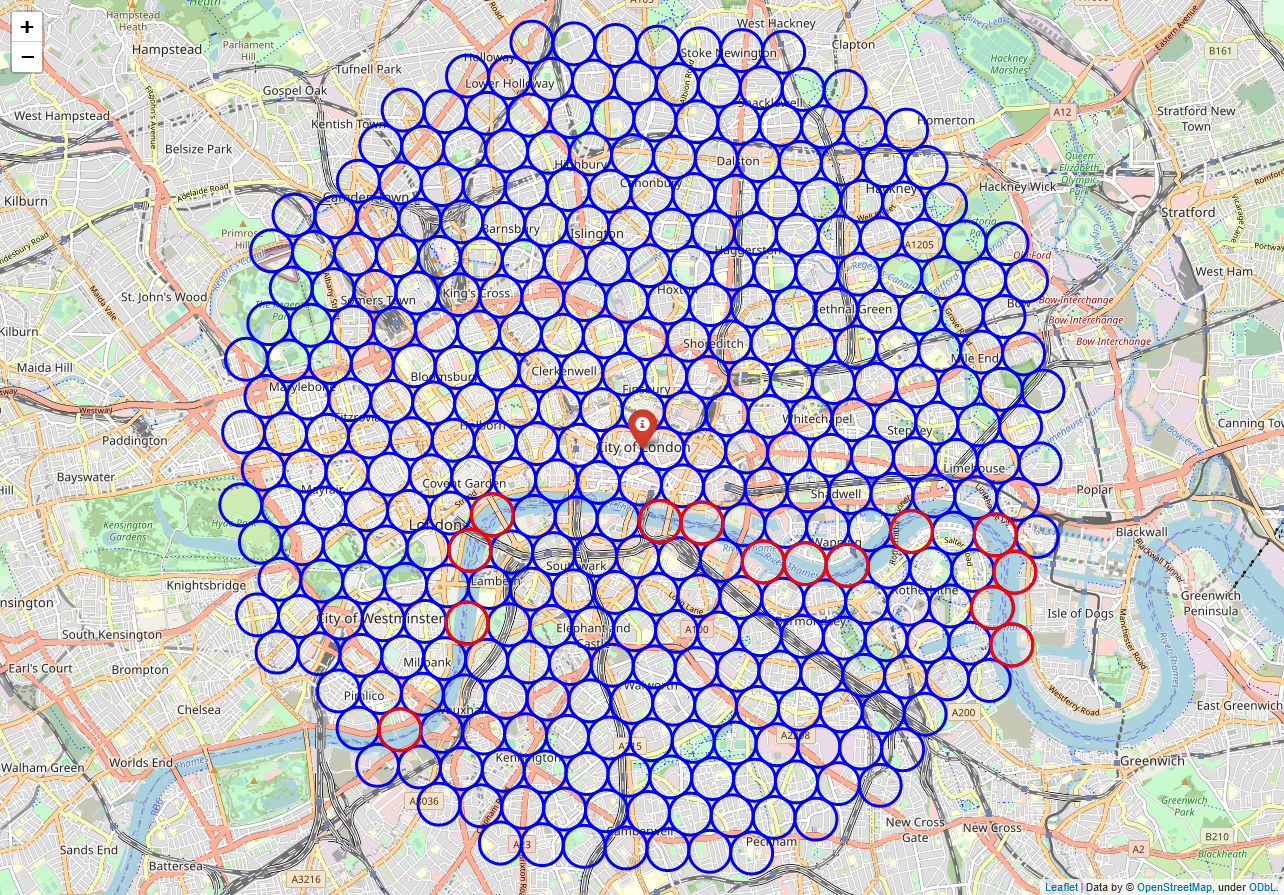
\includegraphics{06_hexa_areas_bad}\end{center}

            % \begin{tcolorbox}[breakable, size=fbox, boxrule=.5pt, pad at break*=1mm, opacityfill=0]
% % \prompt{Out}{outcolor}{49}{\boxspacing}
% \begin{Verbatim}[commandchars=\\\{\}]
% <folium.folium.Map at 0x221e9f250d0>
% \end{Verbatim}
% \end{tcolorbox}
        
    % \begin{tcolorbox}[breakable, size=fbox, boxrule=1pt, pad at break*=1mm,colback=cellbackground, colframe=cellborder]
% \prompt{In}{incolor}{50}{\boxspacing}
% \begin{Verbatim}[commandchars=\\\{\}]
% \PY{n}{save\PYZus{}map}\PY{p}{(}\PY{n}{map\PYZus{}hexa\PYZus{}bad}\PY{p}{,} \PY{l+s+s1}{\PYZsq{}}\PY{l+s+s1}{06\PYZus{}hexa\PYZus{}areas\PYZus{}bad}\PY{l+s+s1}{\PYZsq{}}\PY{p}{)}
% \end{Verbatim}
% \end{tcolorbox}

    % \begin{Verbatim}[commandchars=\\\{\}]
% Map saved under '06\_hexa\_areas\_bad.html' and '06\_hexa\_areas\_bad.png'
    % \end{Verbatim}

    Perfect.

Now it could be great to superpose these on our previous maps containing
the bourough boundaries, still keeping the City of London in red:

    % \begin{tcolorbox}[breakable, size=fbox, boxrule=1pt, pad at break*=1mm,colback=cellbackground, colframe=cellborder]
% \prompt{In}{incolor}{51}{\boxspacing}
% \begin{Verbatim}[commandchars=\\\{\}]
% \PY{n}{map\PYZus{}hexa\PYZus{}city} \PY{o}{=} \PY{n}{folium}\PY{o}{.}\PY{n}{Map}\PY{p}{(}\PY{n}{location}\PY{o}{=}\PY{p}{[}\PY{n}{city\PYZus{}latitude}\PY{p}{,} \PY{n}{city\PYZus{}longitude}\PY{p}{]}\PY{p}{,} \PY{n}{tiles}\PY{o}{=}\PY{l+s+s1}{\PYZsq{}}\PY{l+s+s1}{OpenStreetMap}\PY{l+s+s1}{\PYZsq{}}\PY{p}{,} \PY{n}{zoom\PYZus{}start}\PY{o}{=}\PY{l+m+mi}{13}\PY{p}{)}

% \PY{c+c1}{\PYZsh{} City center}
% \PY{n}{folium}\PY{o}{.}\PY{n}{Marker}\PY{p}{(}\PY{p}{[}\PY{n}{city\PYZus{}latitude}\PY{p}{,} \PY{n}{city\PYZus{}longitude}\PY{p}{]}\PY{p}{,} \PY{n}{icon}\PY{o}{=}\PY{n}{folium}\PY{o}{.}\PY{n}{Icon}\PY{p}{(}\PY{n}{color}\PY{o}{=}\PY{l+s+s1}{\PYZsq{}}\PY{l+s+s1}{red}\PY{l+s+s1}{\PYZsq{}}\PY{p}{,} \PY{n}{icon}\PY{o}{=}\PY{l+s+s1}{\PYZsq{}}\PY{l+s+s1}{info\PYZhy{}sign}\PY{l+s+s1}{\PYZsq{}}\PY{p}{)}\PY{p}{,} \PY{n}{popup}\PY{o}{=}\PY{l+s+s1}{\PYZsq{}}\PY{l+s+s1}{City Center}\PY{l+s+s1}{\PYZsq{}}\PY{p}{)}\PY{o}{.}\PY{n}{add\PYZus{}to}\PY{p}{(}\PY{n}{map\PYZus{}hexa\PYZus{}city}\PY{p}{)}

% \PY{c+c1}{\PYZsh{} Choropleth}

% \PY{n}{folium}\PY{o}{.}\PY{n}{Choropleth}\PY{p}{(}
    % \PY{n}{geo\PYZus{}data}\PY{o}{=}\PY{n}{url\PYZus{}geolondon}\PY{p}{,}
    % \PY{n}{data}\PY{o}{=}\PY{n}{inner\PYZus{}london\PYZus{}data}\PY{p}{,}
    % \PY{n}{columns}\PY{o}{=}\PY{p}{[}\PY{l+s+s1}{\PYZsq{}}\PY{l+s+s1}{Borough}\PY{l+s+s1}{\PYZsq{}}\PY{p}{,} \PY{l+s+s1}{\PYZsq{}}\PY{l+s+s1}{City}\PY{l+s+s1}{\PYZsq{}}\PY{p}{]}\PY{p}{,}
    % \PY{n}{key\PYZus{}on}\PY{o}{=}\PY{l+s+s1}{\PYZsq{}}\PY{l+s+s1}{feature.properties.name}\PY{l+s+s1}{\PYZsq{}}\PY{p}{,}
    % \PY{n}{fill\PYZus{}color}\PY{o}{=}\PY{l+s+s1}{\PYZsq{}}\PY{l+s+s1}{YlOrRd}\PY{l+s+s1}{\PYZsq{}}\PY{p}{,} 
    % \PY{n}{fill\PYZus{}opacity}\PY{o}{=}\PY{l+m+mf}{0.7}\PY{p}{,} 
    % \PY{n}{line\PYZus{}opacity}\PY{o}{=}\PY{l+m+mf}{0.2}\PY{p}{,}
    % \PY{n}{reset}\PY{o}{=}\PY{k+kc}{True}
% \PY{p}{)}\PY{o}{.}\PY{n}{add\PYZus{}to}\PY{p}{(}\PY{n}{map\PYZus{}hexa\PYZus{}city}\PY{p}{)}

% \PY{c+c1}{\PYZsh{} Neighborhoods}
% \PY{k}{for} \PY{n}{lat}\PY{p}{,} \PY{n}{lng}\PY{p}{,} \PY{n}{borough}\PY{p}{,} \PY{n}{neighborhood} \PY{o+ow}{in} \PY{n+nb}{zip}\PY{p}{(}\PY{n}{inner\PYZus{}london\PYZus{}data}\PY{p}{[}\PY{l+s+s1}{\PYZsq{}}\PY{l+s+s1}{Latitude}\PY{l+s+s1}{\PYZsq{}}\PY{p}{]}\PY{p}{,} \PY{n}{inner\PYZus{}london\PYZus{}data}\PY{p}{[}\PY{l+s+s1}{\PYZsq{}}\PY{l+s+s1}{Longitude}\PY{l+s+s1}{\PYZsq{}}\PY{p}{]}\PY{p}{,} \PY{n}{inner\PYZus{}london\PYZus{}data}\PY{p}{[}\PY{l+s+s1}{\PYZsq{}}\PY{l+s+s1}{Borough}\PY{l+s+s1}{\PYZsq{}}\PY{p}{]}\PY{p}{,} \PY{n}{inner\PYZus{}london\PYZus{}data}\PY{p}{[}\PY{l+s+s1}{\PYZsq{}}\PY{l+s+s1}{Neighborhood}\PY{l+s+s1}{\PYZsq{}}\PY{p}{]}\PY{p}{)}\PY{p}{:}
    % \PY{n}{label} \PY{o}{=} \PY{l+s+s1}{\PYZsq{}}\PY{l+s+si}{\PYZob{}\PYZcb{}}\PY{l+s+s1}{, }\PY{l+s+si}{\PYZob{}\PYZcb{}}\PY{l+s+s1}{\PYZsq{}}\PY{o}{.}\PY{n}{format}\PY{p}{(}\PY{n}{neighborhood}\PY{p}{,} \PY{n}{borough}\PY{p}{)}
    % \PY{n}{label} \PY{o}{=} \PY{n}{folium}\PY{o}{.}\PY{n}{Popup}\PY{p}{(}\PY{n}{label}\PY{p}{,} \PY{n}{parse\PYZus{}html}\PY{o}{=}\PY{k+kc}{True}\PY{p}{)}
    % \PY{n}{folium}\PY{o}{.}\PY{n}{CircleMarker}\PY{p}{(}
        % \PY{p}{[}\PY{n}{lat}\PY{p}{,} \PY{n}{lng}\PY{p}{]}\PY{p}{,}
        % \PY{n}{radius}\PY{o}{=}\PY{l+m+mi}{5}\PY{p}{,}
        % \PY{n}{popup}\PY{o}{=}\PY{n}{label}\PY{p}{,}
        % \PY{n}{color}\PY{o}{=}\PY{l+s+s1}{\PYZsq{}}\PY{l+s+s1}{green}\PY{l+s+s1}{\PYZsq{}}\PY{p}{,}
        % \PY{n}{fill}\PY{o}{=}\PY{k+kc}{True}\PY{p}{,}
        % \PY{n}{fill\PYZus{}color}\PY{o}{=}\PY{l+s+s1}{\PYZsq{}}\PY{l+s+s1}{\PYZsh{}3186cc}\PY{l+s+s1}{\PYZsq{}}\PY{p}{,}
        % \PY{n}{fill\PYZus{}opacity}\PY{o}{=}\PY{l+m+mf}{0.7}\PY{p}{,}
        % \PY{n}{parse\PYZus{}html}\PY{o}{=}\PY{k+kc}{False}\PY{p}{)}\PY{o}{.}\PY{n}{add\PYZus{}to}\PY{p}{(}\PY{n}{map\PYZus{}hexa\PYZus{}city}\PY{p}{)}

% \PY{c+c1}{\PYZsh{} All}
% \PY{k}{for} \PY{n}{lat}\PY{p}{,} \PY{n}{lon} \PY{o+ow}{in} \PY{n+nb}{zip}\PY{p}{(}\PY{n}{lat\PYZus{}all}\PY{p}{,} \PY{n}{long\PYZus{}all}\PY{p}{)}\PY{p}{:}
    % \PY{n}{folium}\PY{o}{.}\PY{n}{Circle}\PY{p}{(}\PY{p}{[}\PY{n}{lat}\PY{p}{,} \PY{n}{lon}\PY{p}{]}\PY{p}{,} \PY{n}{radius}\PY{o}{=}\PY{l+m+mi}{250}\PY{p}{,} \PY{n}{color}\PY{o}{=}\PY{l+s+s1}{\PYZsq{}}\PY{l+s+s1}{blue}\PY{l+s+s1}{\PYZsq{}}\PY{p}{,} \PY{n}{fill}\PY{o}{=}\PY{k+kc}{False}\PY{p}{)}\PY{o}{.}\PY{n}{add\PYZus{}to}\PY{p}{(}\PY{n}{map\PYZus{}hexa\PYZus{}city}\PY{p}{)}

% \PY{c+c1}{\PYZsh{} Bad}
% \PY{k}{for} \PY{n}{lat}\PY{p}{,} \PY{n}{lon} \PY{o+ow}{in} \PY{n+nb}{zip}\PY{p}{(}\PY{n}{lat\PYZus{}bad}\PY{p}{,} \PY{n}{long\PYZus{}bad}\PY{p}{)}\PY{p}{:}
    % \PY{c+c1}{\PYZsh{}folium.CircleMarker([lat, lon], radius=2, color=\PYZsq{}blue\PYZsq{}, fill=True, fill\PYZus{}color=\PYZsq{}blue\PYZsq{}, fill\PYZus{}opacity=1).add\PYZus{}to(map\PYZus{}berlin) }
    % \PY{n}{folium}\PY{o}{.}\PY{n}{Circle}\PY{p}{(}\PY{p}{[}\PY{n}{lat}\PY{p}{,} \PY{n}{lon}\PY{p}{]}\PY{p}{,} \PY{n}{radius}\PY{o}{=}\PY{l+m+mi}{250}\PY{p}{,} \PY{n}{color}\PY{o}{=}\PY{l+s+s1}{\PYZsq{}}\PY{l+s+s1}{red}\PY{l+s+s1}{\PYZsq{}}\PY{p}{,} \PY{n}{fill}\PY{o}{=}\PY{k+kc}{False}\PY{p}{)}\PY{o}{.}\PY{n}{add\PYZus{}to}\PY{p}{(}\PY{n}{map\PYZus{}hexa\PYZus{}city}\PY{p}{)}
    % \PY{c+c1}{\PYZsh{}folium.Marker([lat, lon]).add\PYZus{}to(map\PYZus{}berlin)    }

% \PY{c+c1}{\PYZsh{} Display all}
% \PY{n}{map\PYZus{}hexa\PYZus{}city}
% \end{Verbatim}
% \end{tcolorbox}

\begin{center}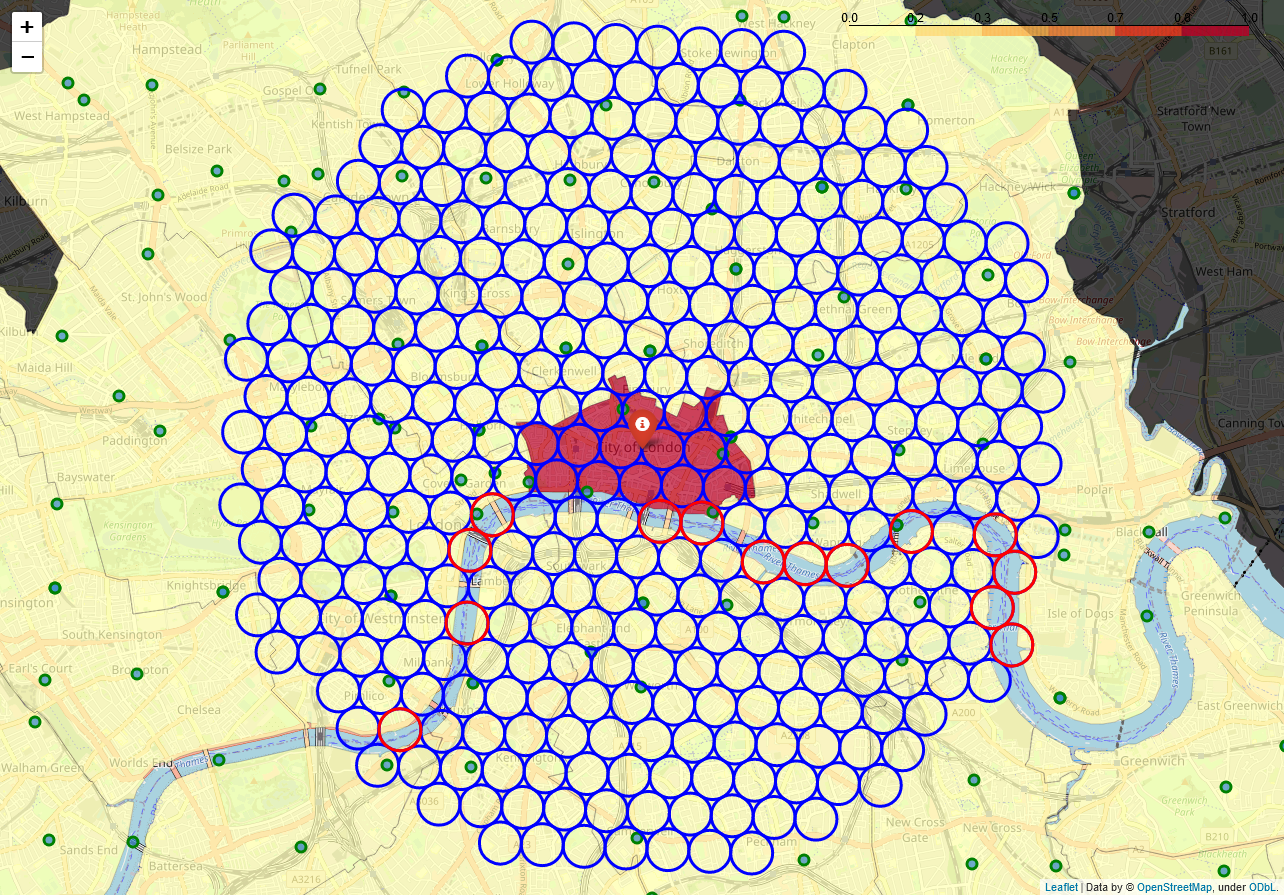
\includegraphics{07_hexa_areas_boundaries}\end{center}

            % \begin{tcolorbox}[breakable, size=fbox, boxrule=.5pt, pad at break*=1mm, opacityfill=0]
% % \prompt{Out}{outcolor}{51}{\boxspacing}
% \begin{Verbatim}[commandchars=\\\{\}]
% <folium.folium.Map at 0x221ea639e20>
% \end{Verbatim}
% \end{tcolorbox}
        
    % \begin{tcolorbox}[breakable, size=fbox, boxrule=1pt, pad at break*=1mm,colback=cellbackground, colframe=cellborder]
% \prompt{In}{incolor}{52}{\boxspacing}
% \begin{Verbatim}[commandchars=\\\{\}]
% \PY{n}{save\PYZus{}map}\PY{p}{(}\PY{n}{map\PYZus{}hexa\PYZus{}city}\PY{p}{,} \PY{l+s+s1}{\PYZsq{}}\PY{l+s+s1}{07\PYZus{}hexa\PYZus{}areas\PYZus{}boundaries}\PY{l+s+s1}{\PYZsq{}}\PY{p}{)}
% \end{Verbatim}
% \end{tcolorbox}

    % \begin{Verbatim}[commandchars=\\\{\}]
% Map saved under '07\_hexa\_areas\_boundaries.html' and
% '07\_hexa\_areas\_boundaries.png'
    % \end{Verbatim}

    Looking good. We can clearly see that our areas covers the whole City of
London, but also spread nicely around it. We will be able to use in
order to find the best places for our restaurant.

But first, let's store our areas coordinates into a dataframe:

    % \begin{tcolorbox}[breakable, size=fbox, boxrule=1pt, pad at break*=1mm,colback=cellbackground, colframe=cellborder]
% \prompt{In}{incolor}{53}{\boxspacing}
% \begin{Verbatim}[commandchars=\\\{\}]
% \PY{n}{hexa} \PY{o}{=} \PY{n}{pd}\PY{o}{.}\PY{n}{merge}\PY{p}{(}\PY{n}{hexa\PYZus{}all}\PY{p}{,}\PY{n}{hexa\PYZus{}bad}\PY{p}{,} \PY{n}{indicator}\PY{o}{=}\PY{k+kc}{True}\PY{p}{,} \PY{n}{how}\PY{o}{=}\PY{l+s+s1}{\PYZsq{}}\PY{l+s+s1}{outer}\PY{l+s+s1}{\PYZsq{}}\PY{p}{)}\PY{o}{.}\PY{n}{query}\PY{p}{(}\PY{l+s+s1}{\PYZsq{}}\PY{l+s+s1}{\PYZus{}merge==}\PY{l+s+s1}{\PYZdq{}}\PY{l+s+s1}{left\PYZus{}only}\PY{l+s+s1}{\PYZdq{}}\PY{l+s+s1}{\PYZsq{}}\PY{p}{)}\PY{o}{.}\PY{n}{drop}\PY{p}{(}\PY{l+s+s1}{\PYZsq{}}\PY{l+s+s1}{\PYZus{}merge}\PY{l+s+s1}{\PYZsq{}}\PY{p}{,} \PY{n}{axis}\PY{o}{=}\PY{l+m+mi}{1}\PY{p}{)}\PY{o}{.}\PY{n}{reset\PYZus{}index}\PY{p}{(}\PY{n}{drop}\PY{o}{=}\PY{k+kc}{True}\PY{p}{)}
% \PY{n+nb}{print}\PY{p}{(}\PY{l+s+s2}{\PYZdq{}}\PY{l+s+s2}{Dataframe shape: }\PY{l+s+si}{\PYZob{}\PYZcb{}}\PY{l+s+s2}{\PYZdq{}}\PY{o}{.}\PY{n}{format}\PY{p}{(}\PY{n}{hexa}\PY{o}{.}\PY{n}{shape}\PY{p}{)}\PY{p}{)}
% \PY{n}{hexa}\PY{o}{.}\PY{n}{head}\PY{p}{(}\PY{p}{)}
% \end{Verbatim}
% \end{tcolorbox}

\resizebox{\textwidth}{!}{%
    \begin{tabular}{lllll}
    Dataframe shape: (350, 5)
    \\ \hline
    Latitude & Longitude & Distance from Center & X & Y
    \\ \hline
    51.473259 & -0.116492 & 4993.746089 & 700250.415693 & 5.706399e+06
    \\
    51.473082 & -0.109302 & 4866.980583 & 700750.415693 & 5.706399e+06
    \\
    51.472904 & -0.102112 & 4789.311015 & 701250.415693 & 5.706399e+06
    \\
    51.472726 & -0.094922 & 4763.139721 & 701750.415693 & 5.706399e+06
    \\
    51.472548 & -0.087733 & 4789.311015 & 702250.415693 & 5.706399e+06
    \end{tabular}
}

    % \begin{Verbatim}[commandchars=\\\{\}]
% Dataframe shape: (350, 5)
    % \end{Verbatim}

            % \begin{tcolorbox}[breakable, size=fbox, boxrule=.5pt, pad at break*=1mm, opacityfill=0]
% % \prompt{Out}{outcolor}{53}{\boxspacing}
% \begin{Verbatim}[commandchars=\\\{\}]
    % Latitude  Longitude  Distance from Center              X             Y
% 0  51.473259  -0.116492           4993.746089  700250.415693  5.706399e+06
% 1  51.473082  -0.109302           4866.980583  700750.415693  5.706399e+06
% 2  51.472904  -0.102112           4789.311015  701250.415693  5.706399e+06
% 3  51.472726  -0.094922           4763.139721  701750.415693  5.706399e+06
% 4  51.472548  -0.087733           4789.311015  702250.415693  5.706399e+06
% \end{Verbatim}
% \end{tcolorbox}
        
    Now, it would be best if we could add another column to it, with the
addresses linked to the given coordinates.

Let's first define a function that will do it, using the Reverse
Geocoding function of the Geocoder library. Let's also test it with the
coordinates of the city center we calculated prior on:

    % \begin{tcolorbox}[breakable, size=fbox, boxrule=1pt, pad at break*=1mm,colback=cellbackground, colframe=cellborder]
% \prompt{In}{incolor}{54}{\boxspacing}
% \begin{Verbatim}[commandchars=\\\{\}]
% \PY{k}{def} \PY{n+nf}{get\PYZus{}address}\PY{p}{(}\PY{n}{lat}\PY{p}{,} \PY{n}{long}\PY{p}{)}\PY{p}{:}
    % \PY{n}{g} \PY{o}{=} \PY{n}{geocoder}\PY{o}{.}\PY{n}{osm}\PY{p}{(}\PY{p}{[}\PY{n}{lat}\PY{p}{,} \PY{n}{long}\PY{p}{]}\PY{p}{,} \PY{n}{method}\PY{o}{=}\PY{l+s+s1}{\PYZsq{}}\PY{l+s+s1}{reverse}\PY{l+s+s1}{\PYZsq{}}\PY{p}{)}
    % \PY{k}{return} \PY{n}{g}\PY{o}{.}\PY{n}{json}\PY{p}{[}\PY{l+s+s1}{\PYZsq{}}\PY{l+s+s1}{address}\PY{l+s+s1}{\PYZsq{}}\PY{p}{]}
% \PY{c+c1}{\PYZsh{} Test}
% \PY{n+nb}{print}\PY{p}{(}\PY{l+s+s2}{\PYZdq{}}\PY{l+s+s2}{City center coordinates address:}\PY{l+s+s2}{\PYZdq{}}\PY{p}{)}
% \PY{n}{get\PYZus{}address}\PY{p}{(}\PY{n}{city\PYZus{}latitude}\PY{p}{,} \PY{n}{city\PYZus{}longitude}\PY{p}{)}
% \end{Verbatim}
% \end{tcolorbox}

    \begin{Verbatim}[commandchars=\\\{\}]
City center coordinates address:
    \end{Verbatim}

            \begin{tcolorbox}[breakable, size=fbox, boxrule=.5pt, pad at break*=1mm, opacityfill=0]
% \prompt{Out}{outcolor}{54}{\boxspacing}
\begin{Verbatim}[commandchars=\\\{\}]
'Roman Amphitheatre Site, Guildhall Yard, Barbican, City of London, Greater
London, England, United Kingdom'
\end{Verbatim}
\end{tcolorbox}
        
    Looking good. Let's now apply this function to our dataframe, and
retrieve the addresses of each rows:

    % \begin{tcolorbox}[breakable, size=fbox, boxrule=1pt, pad at break*=1mm,colback=cellbackground, colframe=cellborder]
% \prompt{In}{incolor}{55}{\boxspacing}
% \begin{Verbatim}[commandchars=\\\{\}]
% \PY{n}{hexa}\PY{p}{[}\PY{l+s+s1}{\PYZsq{}}\PY{l+s+s1}{Address}\PY{l+s+s1}{\PYZsq{}}\PY{p}{]} \PY{o}{=} \PY{n}{hexa}\PY{o}{.}\PY{n}{apply}\PY{p}{(}\PY{k}{lambda} \PY{n}{x}\PY{p}{:} \PY{n}{get\PYZus{}address}\PY{p}{(}\PY{n}{x}\PY{p}{[}\PY{l+s+s1}{\PYZsq{}}\PY{l+s+s1}{Latitude}\PY{l+s+s1}{\PYZsq{}}\PY{p}{]}\PY{p}{,} \PY{n}{x}\PY{p}{[}\PY{l+s+s1}{\PYZsq{}}\PY{l+s+s1}{Longitude}\PY{l+s+s1}{\PYZsq{}}\PY{p}{]}\PY{p}{)}\PY{p}{,} \PY{n}{axis}\PY{o}{=}\PY{l+m+mi}{1}\PY{p}{)}
% \PY{n}{hexa} \PY{o}{=} \PY{n}{hexa}\PY{p}{[}\PY{p}{[}\PY{l+s+s1}{\PYZsq{}}\PY{l+s+s1}{Address}\PY{l+s+s1}{\PYZsq{}}\PY{p}{,}\PY{l+s+s1}{\PYZsq{}}\PY{l+s+s1}{Latitude}\PY{l+s+s1}{\PYZsq{}}\PY{p}{,}\PY{l+s+s1}{\PYZsq{}}\PY{l+s+s1}{Longitude}\PY{l+s+s1}{\PYZsq{}}\PY{p}{,}\PY{l+s+s1}{\PYZsq{}}\PY{l+s+s1}{Distance from Center}\PY{l+s+s1}{\PYZsq{}}\PY{p}{,}\PY{l+s+s1}{\PYZsq{}}\PY{l+s+s1}{X}\PY{l+s+s1}{\PYZsq{}}\PY{p}{,}\PY{l+s+s1}{\PYZsq{}}\PY{l+s+s1}{Y}\PY{l+s+s1}{\PYZsq{}}\PY{p}{]}\PY{p}{]}

% \PY{c+c1}{\PYZsh{} Check}
% \PY{n+nb}{print}\PY{p}{(}\PY{l+s+s2}{\PYZdq{}}\PY{l+s+s2}{Dataframe shape: }\PY{l+s+si}{\PYZob{}\PYZcb{}}\PY{l+s+s2}{\PYZdq{}}\PY{o}{.}\PY{n}{format}\PY{p}{(}\PY{n}{hexa}\PY{o}{.}\PY{n}{shape}\PY{p}{)}\PY{p}{)}
% \PY{n}{hexa}\PY{o}{.}\PY{n}{head}\PY{p}{(}\PY{p}{)}
% \end{Verbatim}
% \end{tcolorbox}

\resizebox{\textwidth}{!}{%
    \begin{tabular}{llllll}
    Dataframe shape: (350, 6)
    \\ \hline
    Addres &
    Latitude & Longitude & Distance from Center & X & Y
    \\ \hline
    Lambeth day nursery, Stockwell Park Road, Stoc{\ldots} &
    51.473259 & -0.116492 & 4993.746089 & 700250.415693 & 5.706399e+06
    \\
    Dundas Road, Kennington, London Borough of Lam{\ldots} &
    51.473082 & -0.109302 & 4866.980583 & 700750.415693 & 5.706399e+06
    \\
    2-4, Welby Street, Paulet Road Estate, Kenning{\ldots} &
    51.472904 & -0.102112 & 4789.311015 & 701250.415693 & 5.706399e+06
    \\
    40, Valmar Road, Camberwell, London Borough of{\ldots} &
    51.472726 & -0.094922 & 4763.139721 & 701750.415693 & 5.706399e+06
    \\
    4-8, Ribbon Dance Mews, Camberwell, London Bor{\ldots} &
    51.472548 & -0.087733 & 4789.311015 & 702250.415693 & 5.706399e+06
    \end{tabular}
}

    % \begin{Verbatim}[commandchars=\\\{\}]
% Dataframe shape: (350, 6)
    % \end{Verbatim}

            % \begin{tcolorbox}[breakable, size=fbox, boxrule=.5pt, pad at break*=1mm, opacityfill=0]
% % \prompt{Out}{outcolor}{55}{\boxspacing}
% \begin{Verbatim}[commandchars=\\\{\}]
                                             % Address   Latitude  Longitude  \textbackslash{}
% 0  Lambeth day nursery, Stockwell Park Road, Stoc{\ldots}  51.473259  -0.116492
% 1  Dundas Road, Kennington, London Borough of Lam{\ldots}  51.473082  -0.109302
% 2  2-4, Welby Street, Paulet Road Estate, Kenning{\ldots}  51.472904  -0.102112
% 3  40, Valmar Road, Camberwell, London Borough of{\ldots}  51.472726  -0.094922
% 4  4-8, Ribbon Dance Mews, Camberwell, London Bor{\ldots}  51.472548  -0.087733

   % Distance from Center              X             Y
% 0           4993.746089  700250.415693  5.706399e+06
% 1           4866.980583  700750.415693  5.706399e+06
% 2           4789.311015  701250.415693  5.706399e+06
% 3           4763.139721  701750.415693  5.706399e+06
% 4           4789.311015  702250.415693  5.706399e+06
% \end{Verbatim}
% \end{tcolorbox}
        
    The results are satisfying. We can now skip to the next step of our data
handling.

    \hypertarget{leveraging-the-foursquare-api}{%
\subsection{Leveraging the Foursquare
API}\label{leveraging-the-foursquare-api}}

Using the Foursquare API, we will retrieve more informations regarding
our neighborhoods.

    In order to use it, we first need to set-up our credentials.

% For confidentiality purposes, we will try to load then from a
% \emph{.env} file, and if no results are retrieved, we prompt for a
% secrured input, using the GetPass library:

    % \begin{tcolorbox}[breakable, size=fbox, boxrule=1pt, pad at break*=1mm,colback=cellbackground, colframe=cellborder]
% \prompt{In}{incolor}{56}{\boxspacing}
% \begin{Verbatim}[commandchars=\\\{\}]
% \PY{c+c1}{\PYZsh{} Try to load .env file}
% \PY{k}{try}\PY{p}{:}
    % \PY{n}{load\PYZus{}dotenv}\PY{p}{(}\PY{p}{)}
    % \PY{n}{CLIENT\PYZus{}ID} \PY{o}{=} \PY{n}{os}\PY{o}{.}\PY{n}{getenv}\PY{p}{(}\PY{l+s+s1}{\PYZsq{}}\PY{l+s+s1}{CLIENT\PYZus{}ID}\PY{l+s+s1}{\PYZsq{}}\PY{p}{)}
    % \PY{n}{CLIENT\PYZus{}SECRET} \PY{o}{=} \PY{n}{os}\PY{o}{.}\PY{n}{getenv}\PY{p}{(}\PY{l+s+s1}{\PYZsq{}}\PY{l+s+s1}{CLIENT\PYZus{}SECRET}\PY{l+s+s1}{\PYZsq{}}\PY{p}{)}
% \PY{c+c1}{\PYZsh{} If no .env file available, ask for user input}
% \PY{k}{except}\PY{p}{:}
    % \PY{n}{CLIENT\PYZus{}ID} \PY{o}{=} \PY{n}{getpass}\PY{o}{.}\PY{n}{getpass}\PY{p}{(}\PY{n}{prompt}\PY{o}{=}\PY{l+s+s2}{\PYZdq{}}\PY{l+s+s2}{Please type your CLIENT\PYZus{}ID: }\PY{l+s+s2}{\PYZdq{}}\PY{p}{)}
    % \PY{n}{CLIENT\PYZus{}SECRET} \PY{o}{=} \PY{n}{getpass}\PY{o}{.}\PY{n}{getpass}\PY{p}{(}\PY{n}{prompt}\PY{o}{=}\PY{l+s+s2}{\PYZdq{}}\PY{l+s+s2}{Please  type your CLIENT\PYZus{}SECRET}\PY{l+s+s2}{\PYZdq{}}\PY{p}{)}

% \PY{c+c1}{\PYZsh{} Other parameters}
% \PY{n}{VERSION} \PY{o}{=} \PY{l+s+s1}{\PYZsq{}}\PY{l+s+s1}{20180605}\PY{l+s+s1}{\PYZsq{}}
% \PY{n}{LIMIT} \PY{o}{=} \PY{l+m+mi}{100}
% \PY{n}{radius} \PY{o}{=} \PY{l+m+mi}{500}

% \PY{c+c1}{\PYZsh{} Print end of credentials}
% \PY{n+nb}{print}\PY{p}{(}\PY{l+s+s1}{\PYZsq{}}\PY{l+s+s1}{Your credentials:}\PY{l+s+s1}{\PYZsq{}}\PY{p}{)}
% \PY{n+nb}{print}\PY{p}{(}\PY{l+s+s1}{\PYZsq{}}\PY{l+s+s1}{CLIENT\PYZus{}ID: }\PY{l+s+si}{\PYZob{}\PYZcb{}}\PY{l+s+si}{\PYZob{}\PYZcb{}}\PY{l+s+s1}{\PYZsq{}}\PY{o}{.}\PY{n}{format}\PY{p}{(}\PY{p}{(}\PY{n+nb}{len}\PY{p}{(}\PY{n}{CLIENT\PYZus{}ID}\PY{p}{)}\PY{o}{\PYZhy{}}\PY{l+m+mi}{4}\PY{p}{)}\PY{o}{*}\PY{l+s+s2}{\PYZdq{}}\PY{l+s+s2}{*}\PY{l+s+s2}{\PYZdq{}}\PY{p}{,} \PY{n}{CLIENT\PYZus{}ID}\PY{p}{[}\PY{o}{\PYZhy{}}\PY{l+m+mi}{4}\PY{p}{:}\PY{p}{]}\PY{p}{)}\PY{p}{)}
% \PY{n+nb}{print}\PY{p}{(}\PY{l+s+s1}{\PYZsq{}}\PY{l+s+s1}{CLIENT\PYZus{}SECRET: }\PY{l+s+si}{\PYZob{}\PYZcb{}}\PY{l+s+si}{\PYZob{}\PYZcb{}}\PY{l+s+s1}{\PYZsq{}}\PY{o}{.}\PY{n}{format}\PY{p}{(}\PY{p}{(}\PY{n+nb}{len}\PY{p}{(}\PY{n}{CLIENT\PYZus{}SECRET}\PY{p}{)}\PY{o}{\PYZhy{}}\PY{l+m+mi}{4}\PY{p}{)}\PY{o}{*}\PY{l+s+s2}{\PYZdq{}}\PY{l+s+s2}{*}\PY{l+s+s2}{\PYZdq{}}\PY{p}{,} \PY{n}{CLIENT\PYZus{}SECRET}\PY{p}{[}\PY{o}{\PYZhy{}}\PY{l+m+mi}{4}\PY{p}{:}\PY{p}{]}\PY{p}{)}\PY{p}{)}
% \end{Verbatim}
% \end{tcolorbox}

    % \begin{Verbatim}[commandchars=\\\{\}]
% Your credentials:
% CLIENT\_ID: ********************************************UXXI
% CLIENT\_SECRET: ********************************************RJLJ
    % \end{Verbatim}

    We're interested in venues in `food' category, but only those that are
proper restaurants. Coffe shops, bakeries, fast-foods etc. are not
direct competitors and shouldn't be taken into account.

We will specifically look for restaurants, and moreover make a
distinction between \textbf{Italian}, \textbf{French}, and others.

    % \begin{tcolorbox}[breakable, size=fbox, boxrule=1pt, pad at break*=1mm,colback=cellbackground, colframe=cellborder]
% \prompt{In}{incolor}{57}{\boxspacing}
% \begin{Verbatim}[commandchars=\\\{\}]
% \PY{c+c1}{\PYZsh{} Category IDs corresponding to Italian restaurants were taken from Foursquare web site (https://developer.foursquare.com/docs/resources/categories):}

% \PY{n}{food\PYZus{}category} \PY{o}{=} \PY{l+s+s1}{\PYZsq{}}\PY{l+s+s1}{4d4b7105d754a06374d81259}\PY{l+s+s1}{\PYZsq{}} \PY{c+c1}{\PYZsh{} \PYZsq{}Root\PYZsq{} category for all food\PYZhy{}related venues}

% \PY{n}{italian\PYZus{}restaurant\PYZus{}categories} \PY{o}{=} \PY{p}{[}\PY{l+s+s1}{\PYZsq{}}\PY{l+s+s1}{4bf58dd8d48988d110941735}\PY{l+s+s1}{\PYZsq{}}\PY{p}{,} \PY{c+c1}{\PYZsh{} Base}
                                 % \PY{l+s+s1}{\PYZsq{}}\PY{l+s+s1}{55a5a1ebe4b013909087cbb6}\PY{l+s+s1}{\PYZsq{}}\PY{p}{,}
                                 % \PY{l+s+s1}{\PYZsq{}}\PY{l+s+s1}{55a5a1ebe4b013909087cb7c}\PY{l+s+s1}{\PYZsq{}}\PY{p}{,}
                                 % \PY{l+s+s1}{\PYZsq{}}\PY{l+s+s1}{55a5a1ebe4b013909087cba7}\PY{l+s+s1}{\PYZsq{}}\PY{p}{,}
                                 % \PY{l+s+s1}{\PYZsq{}}\PY{l+s+s1}{55a5a1ebe4b013909087cba1}\PY{l+s+s1}{\PYZsq{}}\PY{p}{,}
                                 % \PY{l+s+s1}{\PYZsq{}}\PY{l+s+s1}{55a5a1ebe4b013909087cba4}\PY{l+s+s1}{\PYZsq{}}\PY{p}{,}
                                 % \PY{l+s+s1}{\PYZsq{}}\PY{l+s+s1}{55a5a1ebe4b013909087cb95}\PY{l+s+s1}{\PYZsq{}}\PY{p}{,}
                                 % \PY{l+s+s1}{\PYZsq{}}\PY{l+s+s1}{55a5a1ebe4b013909087cb89}\PY{l+s+s1}{\PYZsq{}}\PY{p}{,}
                                 % \PY{l+s+s1}{\PYZsq{}}\PY{l+s+s1}{55a5a1ebe4b013909087cb9b}\PY{l+s+s1}{\PYZsq{}}\PY{p}{,}
                                 % \PY{l+s+s1}{\PYZsq{}}\PY{l+s+s1}{55a5a1ebe4b013909087cb98}\PY{l+s+s1}{\PYZsq{}}\PY{p}{,}
                                 % \PY{l+s+s1}{\PYZsq{}}\PY{l+s+s1}{55a5a1ebe4b013909087cbbf}\PY{l+s+s1}{\PYZsq{}}\PY{p}{,}
                                 % \PY{l+s+s1}{\PYZsq{}}\PY{l+s+s1}{55a5a1ebe4b013909087cb79}\PY{l+s+s1}{\PYZsq{}}\PY{p}{,}
                                 % \PY{l+s+s1}{\PYZsq{}}\PY{l+s+s1}{55a5a1ebe4b013909087cbb0}\PY{l+s+s1}{\PYZsq{}}\PY{p}{,}
                                 % \PY{l+s+s1}{\PYZsq{}}\PY{l+s+s1}{55a5a1ebe4b013909087cbb3}\PY{l+s+s1}{\PYZsq{}}\PY{p}{,}
                                 % \PY{l+s+s1}{\PYZsq{}}\PY{l+s+s1}{55a5a1ebe4b013909087cb74}\PY{l+s+s1}{\PYZsq{}}\PY{p}{,}
                                 % \PY{l+s+s1}{\PYZsq{}}\PY{l+s+s1}{55a5a1ebe4b013909087cbaa}\PY{l+s+s1}{\PYZsq{}}\PY{p}{,}
                                 % \PY{l+s+s1}{\PYZsq{}}\PY{l+s+s1}{55a5a1ebe4b013909087cb83}\PY{l+s+s1}{\PYZsq{}}\PY{p}{,}
                                 % \PY{l+s+s1}{\PYZsq{}}\PY{l+s+s1}{55a5a1ebe4b013909087cb8c}\PY{l+s+s1}{\PYZsq{}}\PY{p}{,}
                                 % \PY{l+s+s1}{\PYZsq{}}\PY{l+s+s1}{55a5a1ebe4b013909087cb92}\PY{l+s+s1}{\PYZsq{}}\PY{p}{,}
                                 % \PY{l+s+s1}{\PYZsq{}}\PY{l+s+s1}{55a5a1ebe4b013909087cb8f}\PY{l+s+s1}{\PYZsq{}}\PY{p}{,}
                                 % \PY{l+s+s1}{\PYZsq{}}\PY{l+s+s1}{55a5a1ebe4b013909087cb86}\PY{l+s+s1}{\PYZsq{}}\PY{p}{,}
                                 % \PY{l+s+s1}{\PYZsq{}}\PY{l+s+s1}{55a5a1ebe4b013909087cbb9}\PY{l+s+s1}{\PYZsq{}}\PY{p}{,}
                                 % \PY{l+s+s1}{\PYZsq{}}\PY{l+s+s1}{55a5a1ebe4b013909087cb7f}\PY{l+s+s1}{\PYZsq{}}\PY{p}{,}
                                 % \PY{l+s+s1}{\PYZsq{}}\PY{l+s+s1}{55a5a1ebe4b013909087cbbc}\PY{l+s+s1}{\PYZsq{}}\PY{p}{,}
                                 % \PY{l+s+s1}{\PYZsq{}}\PY{l+s+s1}{55a5a1ebe4b013909087cb9e}\PY{l+s+s1}{\PYZsq{}}\PY{p}{,}
                                 % \PY{l+s+s1}{\PYZsq{}}\PY{l+s+s1}{55a5a1ebe4b013909087cbc2}\PY{l+s+s1}{\PYZsq{}}\PY{p}{,}
                                 % \PY{l+s+s1}{\PYZsq{}}\PY{l+s+s1}{55a5a1ebe4b013909087cbad}\PY{l+s+s1}{\PYZsq{}}\PY{p}{]}

% \PY{n}{french\PYZus{}restaurant\PYZus{}categories} \PY{o}{=} \PY{p}{[}\PY{l+s+s1}{\PYZsq{}}\PY{l+s+s1}{4bf58dd8d48988d10c941735}\PY{l+s+s1}{\PYZsq{}}\PY{p}{,} \PY{c+c1}{\PYZsh{} Base}
                                % \PY{l+s+s1}{\PYZsq{}}\PY{l+s+s1}{57558b36e4b065ecebd306b6}\PY{l+s+s1}{\PYZsq{}}\PY{p}{,}
                                % \PY{l+s+s1}{\PYZsq{}}\PY{l+s+s1}{57558b36e4b065ecebd306b8}\PY{l+s+s1}{\PYZsq{}}\PY{p}{,}
                                % \PY{l+s+s1}{\PYZsq{}}\PY{l+s+s1}{57558b36e4b065ecebd306bc}\PY{l+s+s1}{\PYZsq{}}\PY{p}{,}
                                % \PY{l+s+s1}{\PYZsq{}}\PY{l+s+s1}{57558b36e4b065ecebd306b0}\PY{l+s+s1}{\PYZsq{}}\PY{p}{,}
                                % \PY{l+s+s1}{\PYZsq{}}\PY{l+s+s1}{57558b36e4b065ecebd306c5}\PY{l+s+s1}{\PYZsq{}}\PY{p}{,}
                                % \PY{l+s+s1}{\PYZsq{}}\PY{l+s+s1}{57558b36e4b065ecebd306c0}\PY{l+s+s1}{\PYZsq{}}\PY{p}{,}
                                % \PY{l+s+s1}{\PYZsq{}}\PY{l+s+s1}{57558b36e4b065ecebd306cb}\PY{l+s+s1}{\PYZsq{}}\PY{p}{,}
                                % \PY{l+s+s1}{\PYZsq{}}\PY{l+s+s1}{57558b36e4b065ecebd306ce}\PY{l+s+s1}{\PYZsq{}}\PY{p}{,}
                                % \PY{l+s+s1}{\PYZsq{}}\PY{l+s+s1}{57558b36e4b065ecebd306d1}\PY{l+s+s1}{\PYZsq{}}\PY{p}{,}
                                % \PY{l+s+s1}{\PYZsq{}}\PY{l+s+s1}{57558b36e4b065ecebd306b4}\PY{l+s+s1}{\PYZsq{}}\PY{p}{,}
                                % \PY{l+s+s1}{\PYZsq{}}\PY{l+s+s1}{57558b36e4b065ecebd306b2}\PY{l+s+s1}{\PYZsq{}}\PY{p}{,}
                                % \PY{l+s+s1}{\PYZsq{}}\PY{l+s+s1}{57558b35e4b065ecebd306ad}\PY{l+s+s1}{\PYZsq{}}\PY{p}{,}
                                % \PY{l+s+s1}{\PYZsq{}}\PY{l+s+s1}{57558b36e4b065ecebd306d4}\PY{l+s+s1}{\PYZsq{}}\PY{p}{,}
                                % \PY{l+s+s1}{\PYZsq{}}\PY{l+s+s1}{57558b36e4b065ecebd306d7}\PY{l+s+s1}{\PYZsq{}}\PY{p}{,}
                                % \PY{l+s+s1}{\PYZsq{}}\PY{l+s+s1}{57558b36e4b065ecebd306da}\PY{l+s+s1}{\PYZsq{}}\PY{p}{,}
                                % \PY{l+s+s1}{\PYZsq{}}\PY{l+s+s1}{57558b36e4b065ecebd306ba}\PY{l+s+s1}{\PYZsq{}}\PY{p}{]}
% \end{Verbatim}
% \end{tcolorbox}

    % \begin{tcolorbox}[breakable, size=fbox, boxrule=1pt, pad at break*=1mm,colback=cellbackground, colframe=cellborder]
% \prompt{In}{incolor}{58}{\boxspacing}
% \begin{Verbatim}[commandchars=\\\{\}]
% \PY{c+c1}{\PYZsh{} Check whether it is a restaurant, and a specific one}
% \PY{k}{def} \PY{n+nf}{is\PYZus{}restaurant}\PY{p}{(}\PY{n}{categories}\PY{p}{,} \PY{n}{specific\PYZus{}filter\PYZus{}one}\PY{o}{=}\PY{k+kc}{None}\PY{p}{,} \PY{n}{specific\PYZus{}filter\PYZus{}two}\PY{o}{=}\PY{k+kc}{None}\PY{p}{)}\PY{p}{:}
    % \PY{n}{restaurant\PYZus{}words} \PY{o}{=} \PY{p}{[}\PY{l+s+s1}{\PYZsq{}}\PY{l+s+s1}{restaurant}\PY{l+s+s1}{\PYZsq{}}\PY{p}{,} \PY{l+s+s1}{\PYZsq{}}\PY{l+s+s1}{diner}\PY{l+s+s1}{\PYZsq{}}\PY{p}{,} \PY{l+s+s1}{\PYZsq{}}\PY{l+s+s1}{taverna}\PY{l+s+s1}{\PYZsq{}}\PY{p}{,} \PY{l+s+s1}{\PYZsq{}}\PY{l+s+s1}{taverne}\PY{l+s+s1}{\PYZsq{}}\PY{p}{,} \PY{l+s+s1}{\PYZsq{}}\PY{l+s+s1}{steakhouse}\PY{l+s+s1}{\PYZsq{}}\PY{p}{,} \PY{l+s+s1}{\PYZsq{}}\PY{l+s+s1}{brasserie}\PY{l+s+s1}{\PYZsq{}}\PY{p}{]}
    % \PY{n}{restaurant} \PY{o}{=} \PY{k+kc}{False}
    % \PY{n}{specific\PYZus{}one} \PY{o}{=} \PY{k+kc}{False}
    % \PY{n}{specific\PYZus{}two} \PY{o}{=} \PY{k+kc}{False}
    % \PY{k}{for} \PY{n}{c} \PY{o+ow}{in} \PY{n}{categories}\PY{p}{:}
        % \PY{n}{category\PYZus{}name} \PY{o}{=} \PY{n}{c}\PY{p}{[}\PY{l+m+mi}{0}\PY{p}{]}\PY{o}{.}\PY{n}{lower}\PY{p}{(}\PY{p}{)}
        % \PY{n}{category\PYZus{}id} \PY{o}{=} \PY{n}{c}\PY{p}{[}\PY{l+m+mi}{1}\PY{p}{]}
        % \PY{k}{for} \PY{n}{r} \PY{o+ow}{in} \PY{n}{restaurant\PYZus{}words}\PY{p}{:}
            % \PY{k}{if} \PY{n}{r} \PY{o+ow}{in} \PY{n}{category\PYZus{}name}\PY{p}{:}
                % \PY{n}{restaurant} \PY{o}{=} \PY{k+kc}{True}
        % \PY{k}{if} \PY{l+s+s1}{\PYZsq{}}\PY{l+s+s1}{fast food}\PY{l+s+s1}{\PYZsq{}} \PY{o+ow}{in} \PY{n}{category\PYZus{}name}\PY{p}{:}
            % \PY{n}{restaurant} \PY{o}{=} \PY{k+kc}{False}
        % \PY{k}{if} \PY{o+ow}{not}\PY{p}{(}\PY{n}{specific\PYZus{}filter\PYZus{}one} \PY{o+ow}{is} \PY{k+kc}{None}\PY{p}{)} \PY{o+ow}{and} \PY{p}{(}\PY{n}{category\PYZus{}id} \PY{o+ow}{in} \PY{n}{specific\PYZus{}filter\PYZus{}one}\PY{p}{)}\PY{p}{:}
            % \PY{n}{specific\PYZus{}one} \PY{o}{=} \PY{k+kc}{True}
            % \PY{n}{specific\PYZus{}two} \PY{o}{=} \PY{k+kc}{False}
            % \PY{n}{restaurant} \PY{o}{=} \PY{k+kc}{True}
        % \PY{k}{if} \PY{o+ow}{not}\PY{p}{(}\PY{n}{specific\PYZus{}filter\PYZus{}two} \PY{o+ow}{is} \PY{k+kc}{None}\PY{p}{)} \PY{o+ow}{and} \PY{p}{(}\PY{n}{category\PYZus{}id} \PY{o+ow}{in} \PY{n}{specific\PYZus{}filter\PYZus{}two}\PY{p}{)}\PY{p}{:}
            % \PY{n}{specific\PYZus{}one} \PY{o}{=} \PY{k+kc}{False}
            % \PY{n}{specific\PYZus{}two} \PY{o}{=} \PY{k+kc}{True}
            % \PY{n}{restaurant} \PY{o}{=} \PY{k+kc}{True} 
    % \PY{k}{return} \PY{n}{restaurant}\PY{p}{,} \PY{n}{specific\PYZus{}one}\PY{p}{,} \PY{n}{specific\PYZus{}two}

% \PY{c+c1}{\PYZsh{} Get category}
% \PY{k}{def} \PY{n+nf}{get\PYZus{}categories}\PY{p}{(}\PY{n}{categories}\PY{p}{)}\PY{p}{:}
    % \PY{k}{return} \PY{p}{[}\PY{p}{(}\PY{n}{cat}\PY{p}{[}\PY{l+s+s1}{\PYZsq{}}\PY{l+s+s1}{name}\PY{l+s+s1}{\PYZsq{}}\PY{p}{]}\PY{p}{,} \PY{n}{cat}\PY{p}{[}\PY{l+s+s1}{\PYZsq{}}\PY{l+s+s1}{id}\PY{l+s+s1}{\PYZsq{}}\PY{p}{]}\PY{p}{)} \PY{k}{for} \PY{n}{cat} \PY{o+ow}{in} \PY{n}{categories}\PY{p}{]}

% \PY{c+c1}{\PYZsh{} Get venues}
% \PY{k}{def} \PY{n+nf}{get\PYZus{}cat\PYZus{}venues}\PY{p}{(}\PY{n}{lat}\PY{p}{,} \PY{n}{lng}\PY{p}{,} \PY{n}{category}\PY{p}{,} \PY{n}{radius}\PY{o}{=}\PY{l+m+mi}{500}\PY{p}{)}\PY{p}{:}
    % \PY{n}{venues\PYZus{}list}\PY{o}{=}\PY{p}{[}\PY{p}{]}
        % \PY{c+c1}{\PYZsh{} create the API request URL}
    % \PY{n}{url} \PY{o}{=} \PY{l+s+s1}{\PYZsq{}}\PY{l+s+s1}{https://api.foursquare.com/v2/venues/explore?\PYZam{}client\PYZus{}id=}\PY{l+s+si}{\PYZob{}\PYZcb{}}\PY{l+s+s1}{\PYZam{}client\PYZus{}secret=}\PY{l+s+si}{\PYZob{}\PYZcb{}}\PY{l+s+s1}{\PYZam{}v=}\PY{l+s+si}{\PYZob{}\PYZcb{}}\PY{l+s+s1}{\PYZam{}ll=}\PY{l+s+si}{\PYZob{}\PYZcb{}}\PY{l+s+s1}{,}\PY{l+s+si}{\PYZob{}\PYZcb{}}\PY{l+s+s1}{\PYZam{}categoryId=}\PY{l+s+si}{\PYZob{}\PYZcb{}}\PY{l+s+s1}{\PYZam{}radius=}\PY{l+s+si}{\PYZob{}\PYZcb{}}\PY{l+s+s1}{\PYZam{}limit=}\PY{l+s+si}{\PYZob{}\PYZcb{}}\PY{l+s+s1}{\PYZsq{}}\PY{o}{.}\PY{n}{format}\PY{p}{(}
        % \PY{n}{CLIENT\PYZus{}ID}\PY{p}{,} 
        % \PY{n}{CLIENT\PYZus{}SECRET}\PY{p}{,} 
        % \PY{n}{VERSION}\PY{p}{,} 
        % \PY{n}{lat}\PY{p}{,} 
        % \PY{n}{lng}\PY{p}{,}
        % \PY{n}{category}\PY{p}{,}
        % \PY{n}{radius}\PY{p}{,} 
        % \PY{n}{LIMIT}\PY{p}{)}
        
    % \PY{k}{try}\PY{p}{:}
        % \PY{n}{results} \PY{o}{=} \PY{n}{requests}\PY{o}{.}\PY{n}{get}\PY{p}{(}\PY{n}{url}\PY{p}{)}\PY{o}{.}\PY{n}{json}\PY{p}{(}\PY{p}{)}\PY{p}{[}\PY{l+s+s2}{\PYZdq{}}\PY{l+s+s2}{response}\PY{l+s+s2}{\PYZdq{}}\PY{p}{]}\PY{p}{[}\PY{l+s+s1}{\PYZsq{}}\PY{l+s+s1}{groups}\PY{l+s+s1}{\PYZsq{}}\PY{p}{]}\PY{p}{[}\PY{l+m+mi}{0}\PY{p}{]}\PY{p}{[}\PY{l+s+s1}{\PYZsq{}}\PY{l+s+s1}{items}\PY{l+s+s1}{\PYZsq{}}\PY{p}{]}
        % \PY{n}{venues\PYZus{}list} \PY{o}{=} \PY{p}{[}\PY{p}{(}\PY{n}{item}\PY{p}{[}\PY{l+s+s1}{\PYZsq{}}\PY{l+s+s1}{venue}\PY{l+s+s1}{\PYZsq{}}\PY{p}{]}\PY{p}{[}\PY{l+s+s1}{\PYZsq{}}\PY{l+s+s1}{id}\PY{l+s+s1}{\PYZsq{}}\PY{p}{]}\PY{p}{,}
                            % \PY{n}{item}\PY{p}{[}\PY{l+s+s1}{\PYZsq{}}\PY{l+s+s1}{venue}\PY{l+s+s1}{\PYZsq{}}\PY{p}{]}\PY{p}{[}\PY{l+s+s1}{\PYZsq{}}\PY{l+s+s1}{name}\PY{l+s+s1}{\PYZsq{}}\PY{p}{]}\PY{p}{,}
                            % \PY{n}{get\PYZus{}categories}\PY{p}{(}\PY{n}{item}\PY{p}{[}\PY{l+s+s1}{\PYZsq{}}\PY{l+s+s1}{venue}\PY{l+s+s1}{\PYZsq{}}\PY{p}{]}\PY{p}{[}\PY{l+s+s1}{\PYZsq{}}\PY{l+s+s1}{categories}\PY{l+s+s1}{\PYZsq{}}\PY{p}{]}\PY{p}{)}\PY{p}{,}
                            % \PY{p}{(}\PY{n}{item}\PY{p}{[}\PY{l+s+s1}{\PYZsq{}}\PY{l+s+s1}{venue}\PY{l+s+s1}{\PYZsq{}}\PY{p}{]}\PY{p}{[}\PY{l+s+s1}{\PYZsq{}}\PY{l+s+s1}{location}\PY{l+s+s1}{\PYZsq{}}\PY{p}{]}\PY{p}{[}\PY{l+s+s1}{\PYZsq{}}\PY{l+s+s1}{lat}\PY{l+s+s1}{\PYZsq{}}\PY{p}{]}\PY{p}{,} \PY{n}{item}\PY{p}{[}\PY{l+s+s1}{\PYZsq{}}\PY{l+s+s1}{venue}\PY{l+s+s1}{\PYZsq{}}\PY{p}{]}\PY{p}{[}\PY{l+s+s1}{\PYZsq{}}\PY{l+s+s1}{location}\PY{l+s+s1}{\PYZsq{}}\PY{p}{]}\PY{p}{[}\PY{l+s+s1}{\PYZsq{}}\PY{l+s+s1}{lng}\PY{l+s+s1}{\PYZsq{}}\PY{p}{]}\PY{p}{)}\PY{p}{,}
                            % \PY{n}{item}\PY{p}{[}\PY{l+s+s1}{\PYZsq{}}\PY{l+s+s1}{venue}\PY{l+s+s1}{\PYZsq{}}\PY{p}{]}\PY{p}{[}\PY{l+s+s1}{\PYZsq{}}\PY{l+s+s1}{location}\PY{l+s+s1}{\PYZsq{}}\PY{p}{]}\PY{p}{,}
                            % \PY{n}{item}\PY{p}{[}\PY{l+s+s1}{\PYZsq{}}\PY{l+s+s1}{venue}\PY{l+s+s1}{\PYZsq{}}\PY{p}{]}\PY{p}{[}\PY{l+s+s1}{\PYZsq{}}\PY{l+s+s1}{location}\PY{l+s+s1}{\PYZsq{}}\PY{p}{]}\PY{p}{[}\PY{l+s+s1}{\PYZsq{}}\PY{l+s+s1}{distance}\PY{l+s+s1}{\PYZsq{}}\PY{p}{]}\PY{p}{)} \PY{k}{for} \PY{n}{item} \PY{o+ow}{in} \PY{n}{results}\PY{p}{]} 
    % \PY{k}{except}\PY{p}{:}
        % \PY{n}{venues\PYZus{}list} \PY{o}{=} \PY{p}{[}\PY{p}{]}
    % \PY{k}{return} \PY{n}{venues\PYZus{}list}

% \PY{c+c1}{\PYZsh{} Restaurants}
% \PY{k}{def} \PY{n+nf}{get\PYZus{}restaurants}\PY{p}{(}\PY{n}{lats}\PY{p}{,} \PY{n}{lons}\PY{p}{)}\PY{p}{:}
    % \PY{n}{restaurants} \PY{o}{=} \PY{p}{\PYZob{}}\PY{p}{\PYZcb{}}
    % \PY{n}{italian\PYZus{}restaurants} \PY{o}{=} \PY{p}{\PYZob{}}\PY{p}{\PYZcb{}}
    % \PY{n}{french\PYZus{}restaurants} \PY{o}{=} \PY{p}{\PYZob{}}\PY{p}{\PYZcb{}}
    % \PY{n}{location\PYZus{}restaurants} \PY{o}{=} \PY{p}{[}\PY{p}{]}

    % \PY{n+nb}{print}\PY{p}{(}\PY{l+s+s1}{\PYZsq{}}\PY{l+s+s1}{Obtaining venues around candidate locations:}\PY{l+s+s1}{\PYZsq{}}\PY{p}{,} \PY{n}{end}\PY{o}{=}\PY{l+s+s1}{\PYZsq{}}\PY{l+s+s1}{\PYZsq{}}\PY{p}{)}
    % \PY{k}{for} \PY{n}{lat}\PY{p}{,} \PY{n}{lon} \PY{o+ow}{in} \PY{n+nb}{zip}\PY{p}{(}\PY{n}{lats}\PY{p}{,} \PY{n}{lons}\PY{p}{)}\PY{p}{:}
        % \PY{c+c1}{\PYZsh{} Using radius=300 to meke sure we have overlaps/full coverage so we don\PYZsq{}t miss any restaurant (we\PYZsq{}re using dictionaries to remove any duplicates resulting from area overlaps)}
        % \PY{n}{venues} \PY{o}{=} \PY{n}{get\PYZus{}cat\PYZus{}venues}\PY{p}{(}\PY{n}{lat}\PY{p}{,} \PY{n}{lon}\PY{p}{,} \PY{n}{food\PYZus{}category}\PY{p}{,} \PY{n}{radius}\PY{o}{=}\PY{l+m+mi}{300}\PY{p}{)}
        % \PY{n}{area\PYZus{}restaurants} \PY{o}{=} \PY{p}{[}\PY{p}{]}
        % \PY{k}{for} \PY{n}{venue} \PY{o+ow}{in} \PY{n}{venues}\PY{p}{:}
            % \PY{n}{venue\PYZus{}id} \PY{o}{=} \PY{n}{venue}\PY{p}{[}\PY{l+m+mi}{0}\PY{p}{]}
            % \PY{n}{venue\PYZus{}name} \PY{o}{=} \PY{n}{venue}\PY{p}{[}\PY{l+m+mi}{1}\PY{p}{]}
            % \PY{n}{venue\PYZus{}categories} \PY{o}{=} \PY{n}{venue}\PY{p}{[}\PY{l+m+mi}{2}\PY{p}{]}
            % \PY{n}{venue\PYZus{}latlon} \PY{o}{=} \PY{n}{venue}\PY{p}{[}\PY{l+m+mi}{3}\PY{p}{]}
            % \PY{n}{venue\PYZus{}address} \PY{o}{=} \PY{n}{venue}\PY{p}{[}\PY{l+m+mi}{4}\PY{p}{]}
            % \PY{n}{venue\PYZus{}distance} \PY{o}{=} \PY{n}{venue}\PY{p}{[}\PY{l+m+mi}{5}\PY{p}{]}
            % \PY{n}{is\PYZus{}res}\PY{p}{,} \PY{n}{is\PYZus{}italian}\PY{p}{,} \PY{n}{is\PYZus{}french} \PY{o}{=} \PY{n}{is\PYZus{}restaurant}\PY{p}{(}\PY{n}{venue\PYZus{}categories}\PY{p}{,} \PY{n}{specific\PYZus{}filter\PYZus{}one}\PY{o}{=}\PY{n}{italian\PYZus{}restaurant\PYZus{}categories}\PY{p}{,} \PY{n}{specific\PYZus{}filter\PYZus{}two}\PY{o}{=}\PY{n}{french\PYZus{}restaurant\PYZus{}categories}\PY{p}{)}
            % \PY{k}{if} \PY{n}{is\PYZus{}res}\PY{p}{:}
                % \PY{n}{x}\PY{p}{,} \PY{n}{y} \PY{o}{=} \PY{n}{lonlat\PYZus{}to\PYZus{}xy}\PY{p}{(}\PY{n}{venue\PYZus{}latlon}\PY{p}{[}\PY{l+m+mi}{1}\PY{p}{]}\PY{p}{,} \PY{n}{venue\PYZus{}latlon}\PY{p}{[}\PY{l+m+mi}{0}\PY{p}{]}\PY{p}{)}
                % \PY{n}{restaurant} \PY{o}{=} \PY{p}{(}\PY{n}{venue\PYZus{}id}\PY{p}{,} \PY{n}{venue\PYZus{}name}\PY{p}{,} \PY{n}{venue\PYZus{}latlon}\PY{p}{[}\PY{l+m+mi}{0}\PY{p}{]}\PY{p}{,} \PY{n}{venue\PYZus{}latlon}\PY{p}{[}\PY{l+m+mi}{1}\PY{p}{]}\PY{p}{,} \PY{n}{venue\PYZus{}address}\PY{p}{,} \PY{n}{venue\PYZus{}distance}\PY{p}{,} \PY{n}{is\PYZus{}italian}\PY{p}{,} \PY{n}{is\PYZus{}french}\PY{p}{,} \PY{n}{x}\PY{p}{,} \PY{n}{y}\PY{p}{)}
                % \PY{k}{if} \PY{n}{venue\PYZus{}distance}\PY{o}{\PYZlt{}}\PY{o}{=}\PY{l+m+mi}{250}\PY{p}{:}
                    % \PY{n}{area\PYZus{}restaurants}\PY{o}{.}\PY{n}{append}\PY{p}{(}\PY{n}{restaurant}\PY{p}{)}
                % \PY{n}{restaurants}\PY{p}{[}\PY{n}{venue\PYZus{}id}\PY{p}{]} \PY{o}{=} \PY{n}{restaurant}
                % \PY{k}{if} \PY{n}{is\PYZus{}italian}\PY{p}{:}
                    % \PY{n}{italian\PYZus{}restaurants}\PY{p}{[}\PY{n}{venue\PYZus{}id}\PY{p}{]} \PY{o}{=} \PY{n}{restaurant}
                % \PY{k}{if} \PY{n}{is\PYZus{}french}\PY{p}{:}
                    % \PY{n}{french\PYZus{}restaurants}\PY{p}{[}\PY{n}{venue\PYZus{}id}\PY{p}{]} \PY{o}{=} \PY{n}{restaurant}
        % \PY{n}{location\PYZus{}restaurants}\PY{o}{.}\PY{n}{append}\PY{p}{(}\PY{n}{area\PYZus{}restaurants}\PY{p}{)}
        % \PY{n+nb}{print}\PY{p}{(}\PY{l+s+s1}{\PYZsq{}}\PY{l+s+s1}{ .}\PY{l+s+s1}{\PYZsq{}}\PY{p}{,} \PY{n}{end}\PY{o}{=}\PY{l+s+s1}{\PYZsq{}}\PY{l+s+s1}{\PYZsq{}}\PY{p}{)}
    % \PY{n+nb}{print}\PY{p}{(}\PY{l+s+s1}{\PYZsq{}}\PY{l+s+s1}{ done.}\PY{l+s+s1}{\PYZsq{}}\PY{p}{)}
    % \PY{k}{return} \PY{n}{restaurants}\PY{p}{,} \PY{n}{italian\PYZus{}restaurants}\PY{p}{,} \PY{n}{french\PYZus{}restaurants}\PY{p}{,} \PY{n}{location\PYZus{}restaurants}
% \end{Verbatim}
% \end{tcolorbox}

    Let's obtain the venues for our areas, using either the Foursquare API,
or, if we had already done so and persisted the results in a Pickle
file, by loading it:

    % \begin{tcolorbox}[breakable, size=fbox, boxrule=1pt, pad at break*=1mm,colback=cellbackground, colframe=cellborder]
% \prompt{In}{incolor}{59}{\boxspacing}
% \begin{Verbatim}[commandchars=\\\{\}]
% \PY{k+kn}{import} \PY{n+nn}{pickle}

% \PY{c+c1}{\PYZsh{} Try to load from local file system in case we did this before}
% \PY{n}{restaurants} \PY{o}{=} \PY{p}{\PYZob{}}\PY{p}{\PYZcb{}}
% \PY{n}{italian\PYZus{}restaurants} \PY{o}{=} \PY{p}{\PYZob{}}\PY{p}{\PYZcb{}}
% \PY{n}{french\PYZus{}restaurants} \PY{o}{=} \PY{p}{\PYZob{}}\PY{p}{\PYZcb{}}
% \PY{n}{location\PYZus{}restaurants} \PY{o}{=} \PY{p}{[}\PY{p}{]}
% \PY{n}{loaded} \PY{o}{=} \PY{k+kc}{False}
% \PY{k}{try}\PY{p}{:}
    % \PY{k}{with} \PY{n+nb}{open}\PY{p}{(}\PY{l+s+s1}{\PYZsq{}}\PY{l+s+s1}{restaurants.pkl}\PY{l+s+s1}{\PYZsq{}}\PY{p}{,} \PY{l+s+s1}{\PYZsq{}}\PY{l+s+s1}{rb}\PY{l+s+s1}{\PYZsq{}}\PY{p}{)} \PY{k}{as} \PY{n}{f}\PY{p}{:}
        % \PY{n}{restaurants} \PY{o}{=} \PY{n}{pickle}\PY{o}{.}\PY{n}{load}\PY{p}{(}\PY{n}{f}\PY{p}{)}
    % \PY{k}{with} \PY{n+nb}{open}\PY{p}{(}\PY{l+s+s1}{\PYZsq{}}\PY{l+s+s1}{italian\PYZus{}restaurants.pkl}\PY{l+s+s1}{\PYZsq{}}\PY{p}{,} \PY{l+s+s1}{\PYZsq{}}\PY{l+s+s1}{rb}\PY{l+s+s1}{\PYZsq{}}\PY{p}{)} \PY{k}{as} \PY{n}{f}\PY{p}{:}
        % \PY{n}{italian\PYZus{}restaurants} \PY{o}{=} \PY{n}{pickle}\PY{o}{.}\PY{n}{load}\PY{p}{(}\PY{n}{f}\PY{p}{)}
    % \PY{k}{with} \PY{n+nb}{open}\PY{p}{(}\PY{l+s+s1}{\PYZsq{}}\PY{l+s+s1}{french\PYZus{}restaurants.pkl}\PY{l+s+s1}{\PYZsq{}}\PY{p}{,} \PY{l+s+s1}{\PYZsq{}}\PY{l+s+s1}{rb}\PY{l+s+s1}{\PYZsq{}}\PY{p}{)} \PY{k}{as} \PY{n}{f}\PY{p}{:}
        % \PY{n}{french\PYZus{}restaurants} \PY{o}{=} \PY{n}{pickle}\PY{o}{.}\PY{n}{load}\PY{p}{(}\PY{n}{f}\PY{p}{)}
    % \PY{k}{with} \PY{n+nb}{open}\PY{p}{(}\PY{l+s+s1}{\PYZsq{}}\PY{l+s+s1}{location\PYZus{}restaurants.pkl}\PY{l+s+s1}{\PYZsq{}}\PY{p}{,} \PY{l+s+s1}{\PYZsq{}}\PY{l+s+s1}{rb}\PY{l+s+s1}{\PYZsq{}}\PY{p}{)} \PY{k}{as} \PY{n}{f}\PY{p}{:}
        % \PY{n}{location\PYZus{}restaurants} \PY{o}{=} \PY{n}{pickle}\PY{o}{.}\PY{n}{load}\PY{p}{(}\PY{n}{f}\PY{p}{)}
    % \PY{n+nb}{print}\PY{p}{(}\PY{l+s+s1}{\PYZsq{}}\PY{l+s+s1}{Restaurant data loaded.}\PY{l+s+s1}{\PYZsq{}}\PY{p}{)}
    % \PY{n}{loaded} \PY{o}{=} \PY{k+kc}{True}
% \PY{k}{except}\PY{p}{:}
    % \PY{k}{pass}

% \PY{c+c1}{\PYZsh{} If load failed use the Foursquare API to get the data}
% \PY{k}{if} \PY{o+ow}{not} \PY{n}{loaded}\PY{p}{:}
    % \PY{n}{restaurants}\PY{p}{,} \PY{n}{italian\PYZus{}restaurants}\PY{p}{,} \PY{n}{french\PYZus{}restaurants}\PY{p}{,} \PY{n}{location\PYZus{}restaurants} \PY{o}{=} \PY{n}{get\PYZus{}restaurants}\PY{p}{(}\PY{n}{hexa}\PY{p}{[}\PY{l+s+s1}{\PYZsq{}}\PY{l+s+s1}{Latitude}\PY{l+s+s1}{\PYZsq{}}\PY{p}{]}\PY{p}{,} \PY{n}{hexa}\PY{p}{[}\PY{l+s+s1}{\PYZsq{}}\PY{l+s+s1}{Longitude}\PY{l+s+s1}{\PYZsq{}}\PY{p}{]}\PY{p}{)}
    
    % \PY{c+c1}{\PYZsh{} Let\PYZsq{}s persists this in local file system}
    % \PY{k}{with} \PY{n+nb}{open}\PY{p}{(}\PY{l+s+s1}{\PYZsq{}}\PY{l+s+s1}{restaurants.pkl}\PY{l+s+s1}{\PYZsq{}}\PY{p}{,} \PY{l+s+s1}{\PYZsq{}}\PY{l+s+s1}{wb}\PY{l+s+s1}{\PYZsq{}}\PY{p}{)} \PY{k}{as} \PY{n}{f}\PY{p}{:}
        % \PY{n}{pickle}\PY{o}{.}\PY{n}{dump}\PY{p}{(}\PY{n}{restaurants}\PY{p}{,} \PY{n}{f}\PY{p}{)}
    % \PY{k}{with} \PY{n+nb}{open}\PY{p}{(}\PY{l+s+s1}{\PYZsq{}}\PY{l+s+s1}{italian\PYZus{}restaurants.pkl}\PY{l+s+s1}{\PYZsq{}}\PY{p}{,} \PY{l+s+s1}{\PYZsq{}}\PY{l+s+s1}{wb}\PY{l+s+s1}{\PYZsq{}}\PY{p}{)} \PY{k}{as} \PY{n}{f}\PY{p}{:}
        % \PY{n}{pickle}\PY{o}{.}\PY{n}{dump}\PY{p}{(}\PY{n}{italian\PYZus{}restaurants}\PY{p}{,} \PY{n}{f}\PY{p}{)}
    % \PY{k}{with} \PY{n+nb}{open}\PY{p}{(}\PY{l+s+s1}{\PYZsq{}}\PY{l+s+s1}{french\PYZus{}restaurants.pkl}\PY{l+s+s1}{\PYZsq{}}\PY{p}{,} \PY{l+s+s1}{\PYZsq{}}\PY{l+s+s1}{wb}\PY{l+s+s1}{\PYZsq{}}\PY{p}{)} \PY{k}{as} \PY{n}{f}\PY{p}{:}
        % \PY{n}{pickle}\PY{o}{.}\PY{n}{dump}\PY{p}{(}\PY{n}{french\PYZus{}restaurants}\PY{p}{,} \PY{n}{f}\PY{p}{)}
    % \PY{k}{with} \PY{n+nb}{open}\PY{p}{(}\PY{l+s+s1}{\PYZsq{}}\PY{l+s+s1}{location\PYZus{}restaurants.pkl}\PY{l+s+s1}{\PYZsq{}}\PY{p}{,} \PY{l+s+s1}{\PYZsq{}}\PY{l+s+s1}{wb}\PY{l+s+s1}{\PYZsq{}}\PY{p}{)} \PY{k}{as} \PY{n}{f}\PY{p}{:}
        % \PY{n}{pickle}\PY{o}{.}\PY{n}{dump}\PY{p}{(}\PY{n}{location\PYZus{}restaurants}\PY{p}{,} \PY{n}{f}\PY{p}{)}
    % \PY{n+nb}{print}\PY{p}{(}\PY{l+s+s1}{\PYZsq{}}\PY{l+s+s1}{Data saved.}\PY{l+s+s1}{\PYZsq{}}\PY{p}{)}
% \end{Verbatim}
% \end{tcolorbox}

    % \begin{Verbatim}[commandchars=\\\{\}]
% Restaurant data loaded.
    % \end{Verbatim}

    Let's have a quick look at our resulting data:

    % \begin{tcolorbox}[breakable, size=fbox, boxrule=1pt, pad at break*=1mm,colback=cellbackground, colframe=cellborder]
% \prompt{In}{incolor}{60}{\boxspacing}
% \begin{Verbatim}[commandchars=\\\{\}]
% \PY{n+nb}{print}\PY{p}{(}\PY{l+s+s1}{\PYZsq{}}\PY{l+s+s1}{Total number of restaurants:}\PY{l+s+s1}{\PYZsq{}}\PY{p}{,} \PY{n+nb}{len}\PY{p}{(}\PY{n}{restaurants}\PY{p}{)}\PY{p}{)}
% \PY{n+nb}{print}\PY{p}{(}\PY{l+s+s1}{\PYZsq{}}\PY{l+s+s1}{Total number of Italian restaurants:}\PY{l+s+s1}{\PYZsq{}}\PY{p}{,} \PY{n+nb}{len}\PY{p}{(}\PY{n}{italian\PYZus{}restaurants}\PY{p}{)}\PY{p}{)}
% \PY{n+nb}{print}\PY{p}{(}\PY{l+s+s1}{\PYZsq{}}\PY{l+s+s1}{Percentage of Italian restaurants: }\PY{l+s+si}{\PYZob{}:.2f\PYZcb{}}\PY{l+s+s1}{\PYZpc{}}\PY{l+s+s1}{\PYZsq{}}\PY{o}{.}\PY{n}{format}\PY{p}{(}\PY{n+nb}{len}\PY{p}{(}\PY{n}{italian\PYZus{}restaurants}\PY{p}{)} \PY{o}{/} \PY{n+nb}{len}\PY{p}{(}\PY{n}{restaurants}\PY{p}{)} \PY{o}{*} \PY{l+m+mi}{100}\PY{p}{)}\PY{p}{)}
% \PY{n+nb}{print}\PY{p}{(}\PY{l+s+s1}{\PYZsq{}}\PY{l+s+s1}{Total number of French restaurants:}\PY{l+s+s1}{\PYZsq{}}\PY{p}{,} \PY{n+nb}{len}\PY{p}{(}\PY{n}{french\PYZus{}restaurants}\PY{p}{)}\PY{p}{)}
% \PY{n+nb}{print}\PY{p}{(}\PY{l+s+s1}{\PYZsq{}}\PY{l+s+s1}{Percentage of French restaurants: }\PY{l+s+si}{\PYZob{}:.2f\PYZcb{}}\PY{l+s+s1}{\PYZpc{}}\PY{l+s+s1}{\PYZsq{}}\PY{o}{.}\PY{n}{format}\PY{p}{(}\PY{n+nb}{len}\PY{p}{(}\PY{n}{french\PYZus{}restaurants}\PY{p}{)} \PY{o}{/} \PY{n+nb}{len}\PY{p}{(}\PY{n}{restaurants}\PY{p}{)} \PY{o}{*} \PY{l+m+mi}{100}\PY{p}{)}\PY{p}{)}
% \PY{n+nb}{print}\PY{p}{(}\PY{l+s+s1}{\PYZsq{}}\PY{l+s+s1}{Average number of restaurants in neighborhood:}\PY{l+s+s1}{\PYZsq{}}\PY{p}{,} \PY{n}{np}\PY{o}{.}\PY{n}{array}\PY{p}{(}\PY{p}{[}\PY{n+nb}{len}\PY{p}{(}\PY{n}{r}\PY{p}{)} \PY{k}{for} \PY{n}{r} \PY{o+ow}{in} \PY{n}{location\PYZus{}restaurants}\PY{p}{]}\PY{p}{)}\PY{o}{.}\PY{n}{mean}\PY{p}{(}\PY{p}{)}\PY{p}{)}
% \end{Verbatim}
% \end{tcolorbox}

    \begin{Verbatim}[commandchars=\\\{\}]
Total number of restaurants: 2223
Total number of Italian restaurants: 295
Percentage of Italian restaurants: 13.27\%
Total number of French restaurants: 116
Percentage of French restaurants: 5.22\%
Average number of restaurants in neighborhood: 5.44
    \end{Verbatim}

    % \begin{tcolorbox}[breakable, size=fbox, boxrule=1pt, pad at break*=1mm,colback=cellbackground, colframe=cellborder]
% \prompt{In}{incolor}{61}{\boxspacing}
% \begin{Verbatim}[commandchars=\\\{\}]
% \PY{n+nb}{print}\PY{p}{(}\PY{l+s+s1}{\PYZsq{}}\PY{l+s+s1}{List of all restaurants}\PY{l+s+s1}{\PYZsq{}}\PY{p}{)}
% \PY{n+nb}{print}\PY{p}{(}\PY{l+s+s1}{\PYZsq{}}\PY{l+s+s1}{\PYZhy{}\PYZhy{}\PYZhy{}\PYZhy{}\PYZhy{}\PYZhy{}\PYZhy{}\PYZhy{}\PYZhy{}\PYZhy{}\PYZhy{}\PYZhy{}\PYZhy{}\PYZhy{}\PYZhy{}\PYZhy{}\PYZhy{}\PYZhy{}\PYZhy{}\PYZhy{}\PYZhy{}\PYZhy{}\PYZhy{}}\PY{l+s+s1}{\PYZsq{}}\PY{p}{)}
% \PY{k}{for} \PY{n}{r} \PY{o+ow}{in} \PY{n+nb}{list}\PY{p}{(}\PY{n}{restaurants}\PY{o}{.}\PY{n}{values}\PY{p}{(}\PY{p}{)}\PY{p}{)}\PY{p}{[}\PY{p}{:}\PY{l+m+mi}{10}\PY{p}{]}\PY{p}{:}
    % \PY{n+nb}{print}\PY{p}{(}\PY{n}{r}\PY{p}{)}
% \PY{n+nb}{print}\PY{p}{(}\PY{l+s+s1}{\PYZsq{}}\PY{l+s+s1}{...}\PY{l+s+s1}{\PYZsq{}}\PY{p}{)}
% \PY{n+nb}{print}\PY{p}{(}\PY{l+s+s1}{\PYZsq{}}\PY{l+s+s1}{Total:}\PY{l+s+s1}{\PYZsq{}}\PY{p}{,} \PY{n+nb}{len}\PY{p}{(}\PY{n}{restaurants}\PY{p}{)}\PY{p}{)}
% \end{Verbatim}
% \end{tcolorbox}

    % \begin{Verbatim}[commandchars=\\\{\}]
% List of all restaurants
% -----------------------
% ('5b77fd3095a722002b2802d5', 'Pipoca Vegan', 51.472065, -0.11278421, \{'address':
% '224 Brixton Rd', 'lat': 51.472065, 'lng': -0.11278421, 'labeledLatLngs':
% [\{'label': 'display', 'lat': 51.472065, 'lng': -0.11278421\}], 'distance': 266,
% 'postalCode': 'SW9', 'cc': 'GB', 'city': 'London', 'state': 'Greater London',
% 'country': 'United Kingdom', 'formattedAddress': ['224 Brixton Rd', 'London',
% 'Greater London', 'SW9', 'United Kingdom']\}, 266, False, False,
% 700513.097289601, 5706276.178980275)
% ('502686ffe4b0f46cce4f6937', 'Vegan and Vegetarian Cuisine', 51.47368215178113,
% -0.11111110385916374, \{'lat': 51.47368215178113, 'lng': -0.11111110385916374,
% 'labeledLatLngs': [\{'label': 'display', 'lat': 51.47368215178113, 'lng':
% -0.11111110385916374\}], 'distance': 142, 'cc': 'GB', 'country': 'United
% Kingdom', 'formattedAddress': ['United Kingdom']\}, 142, False, False,
% 700622.1720664381, 5706460.560765747)
% ('4ea7d623d3e33e1d4f183fd3', 'Garage Canteen', 51.47310883065202,
% -0.09938575231829633, \{'address': 'Warner Rd', 'lat': 51.47310883065202, 'lng':
% -0.09938575231829633, 'labeledLatLngs': [\{'label': 'display', 'lat':
% 51.47310883065202, 'lng': -0.09938575231829633\}], 'distance': 190, 'cc': 'GB',
% 'city': 'Camberwell', 'state': 'Greater London', 'country': 'United Kingdom',
% 'formattedAddress': ['Warner Rd', 'Camberwell', 'Greater London', 'United
% Kingdom']\}, 190, False, False, 701438.8236954896, 5706429.024340321)
% ('4b55f9ccf964a520ebf927e3', "Nando's", 51.47178409795933, -0.0932268780619469,
% \{'address': '88 Denmark Hill', 'lat': 51.47178409795933, 'lng':
% -0.0932268780619469, 'labeledLatLngs': [\{'label': 'display', 'lat':
% 51.47178409795933, 'lng': -0.0932268780619469\}], 'distance': 157, 'postalCode':
% 'SE5 8RX', 'cc': 'GB', 'city': 'Camberwell', 'state': 'Greater London',
% 'country': 'United Kingdom', 'formattedAddress': ['88 Denmark Hill',
% 'Camberwell', 'Greater London', 'SE5 8RX', 'United Kingdom']\}, 157, False,
% False, 701872.3072687672, 5706298.708450208)
% ('4f439648e4b05d3b161b1087', 'Viet Cafe', 51.4710444177932,
% -0.09290986290229072, \{'address': '75 Denmark Hill', 'lat': 51.4710444177932,
% 'lng': -0.09290986290229072, 'labeledLatLngs': [\{'label': 'display', 'lat':
% 51.4710444177932, 'lng': -0.09290986290229072\}], 'distance': 233, 'postalCode':
% 'SE5 8RS', 'cc': 'GB', 'city': 'London', 'state': 'Greater London', 'country':
% 'United Kingdom', 'formattedAddress': ['75 Denmark Hill', 'London', 'Greater
% London', 'SE5 8RS', 'United Kingdom']\}, 233, False, False, 701897.5864545307,
% 5706217.344664776)
% ('4d70323fb73bb1f78f15b672', 'Golden Grill', 51.47411797219679,
% -0.09289607516702363, \{'address': '20 Camberwell Green', 'lat':
% 51.47411797219679, 'lng': -0.09289607516702363, 'labeledLatLngs': [\{'label':
% 'display', 'lat': 51.47411797219679, 'lng': -0.09289607516702363\}], 'distance':
% 296, 'postalCode': 'SE5 7AA', 'cc': 'GB', 'city': 'Camberwell', 'state':
% 'Greater London', 'country': 'United Kingdom', 'formattedAddress': ['20
% Camberwell Green', 'Camberwell', 'Greater London', 'SE5 7AA', 'United
% Kingdom']\}, 296, False, False, 701884.9681498781, 5706559.1028932305)
% ('4c4bc0eb46240f470bc3c1f3', 'Tasty House', 51.47061809639869,
% -0.09291170380092716, \{'address': '118 Denmark Hill', 'lat': 51.47061809639869,
% 'lng': -0.09291170380092716, 'labeledLatLngs': [\{'label': 'display', 'lat':
% 51.47061809639869, 'lng': -0.09291170380092716\}], 'distance': 272, 'postalCode':
% 'SE5 8RX', 'cc': 'GB', 'city': 'Camberwell', 'state': 'Greater London',
% 'country': 'United Kingdom', 'formattedAddress': ['118 Denmark Hill',
% 'Camberwell', 'Greater London', 'SE5 8RX', 'United Kingdom']\}, 272, False,
% False, 701899.341604687, 5706169.940849295)
% ('4d41e8d71da9a09374cd5c3d', 'Indiaah', 51.47159636453626, -0.0930612752686487,
% \{'address': '39 Denmark Hill', 'lat': 51.47159636453626, 'lng':
% -0.0930612752686487, 'labeledLatLngs': [\{'label': 'display', 'lat':
% 51.47159636453626, 'lng': -0.0930612752686487\}], 'distance': 180, 'cc': 'GB',
% 'city': 'London', 'state': 'Greater London', 'country': 'United Kingdom',
% 'formattedAddress': ['39 Denmark Hill', 'London', 'Greater London', 'United
% Kingdom']\}, 180, False, False, 701884.6351465094, 5706278.29287368)
% ('4bdc8cffc79cc928d21487e9', 'Su-Thai', 51.471546, -0.093636, \{'address':
% 'Coldharbour Ln.', 'lat': 51.471546, 'lng': -0.093636, 'labeledLatLngs':
% [\{'label': 'display', 'lat': 51.471546, 'lng': -0.093636\}], 'distance': 158,
% 'postalCode': 'SE5 9PR', 'cc': 'GB', 'city': 'Camberwell', 'state': 'Greater
% London', 'country': 'United Kingdom', 'formattedAddress': ['Coldharbour Ln.',
% 'Camberwell', 'Greater London', 'SE5 9PR', 'United Kingdom']\}, 158, False,
% False, 701844.9510201943, 5706271.108188438)
% ('4c115ef8d917c928f29bb562', 'Lamoon', 51.47209884762519, -0.09308092718313395,
% \{'address': '39 Denmark Hill', 'lat': 51.47209884762519, 'lng':
% -0.09308092718313395, 'labeledLatLngs': [\{'label': 'display', 'lat':
% 51.47209884762519, 'lng': -0.09308092718313395\}], 'distance': 145, 'postalCode':
% 'SE5 8RS', 'cc': 'GB', 'city': 'Camberwell', 'state': 'Greater London',
% 'country': 'United Kingdom', 'formattedAddress': ['39 Denmark Hill',
% 'Camberwell', 'Greater London', 'SE5 8RS', 'United Kingdom']\}, 145, False,
% False, 701881.0513290586, 5706334.105129385)
% {\ldots}
% Total: 2223
    % \end{Verbatim}

    % \begin{tcolorbox}[breakable, size=fbox, boxrule=1pt, pad at break*=1mm,colback=cellbackground, colframe=cellborder]
% \prompt{In}{incolor}{62}{\boxspacing}
% \begin{Verbatim}[commandchars=\\\{\}]
% \PY{n+nb}{print}\PY{p}{(}\PY{l+s+s1}{\PYZsq{}}\PY{l+s+s1}{List of Italian restaurants}\PY{l+s+s1}{\PYZsq{}}\PY{p}{)}
% \PY{n+nb}{print}\PY{p}{(}\PY{l+s+s1}{\PYZsq{}}\PY{l+s+s1}{\PYZhy{}\PYZhy{}\PYZhy{}\PYZhy{}\PYZhy{}\PYZhy{}\PYZhy{}\PYZhy{}\PYZhy{}\PYZhy{}\PYZhy{}\PYZhy{}\PYZhy{}\PYZhy{}\PYZhy{}\PYZhy{}\PYZhy{}\PYZhy{}\PYZhy{}\PYZhy{}\PYZhy{}\PYZhy{}\PYZhy{}\PYZhy{}\PYZhy{}\PYZhy{}\PYZhy{}}\PY{l+s+s1}{\PYZsq{}}\PY{p}{)}
% \PY{k}{for} \PY{n}{r} \PY{o+ow}{in} \PY{n+nb}{list}\PY{p}{(}\PY{n}{italian\PYZus{}restaurants}\PY{o}{.}\PY{n}{values}\PY{p}{(}\PY{p}{)}\PY{p}{)}\PY{p}{[}\PY{p}{:}\PY{l+m+mi}{10}\PY{p}{]}\PY{p}{:}
    % \PY{n+nb}{print}\PY{p}{(}\PY{n}{r}\PY{p}{)}
% \PY{n+nb}{print}\PY{p}{(}\PY{l+s+s1}{\PYZsq{}}\PY{l+s+s1}{...}\PY{l+s+s1}{\PYZsq{}}\PY{p}{)}
% \PY{n+nb}{print}\PY{p}{(}\PY{l+s+s1}{\PYZsq{}}\PY{l+s+s1}{Total:}\PY{l+s+s1}{\PYZsq{}}\PY{p}{,} \PY{n+nb}{len}\PY{p}{(}\PY{n}{italian\PYZus{}restaurants}\PY{p}{)}\PY{p}{)}
% \end{Verbatim}
% \end{tcolorbox}

    % \begin{Verbatim}[commandchars=\\\{\}]
% List of Italian restaurants
% ---------------------------
% ('4b643b46f964a52069a52ae3', 'Caravaggio', 51.473932213286865,
% -0.08938251483507732, \{'address': '47 Camberwell Church Street', 'crossStreet':
% 'Opposite Camberwell Grove', 'lat': 51.473932213286865, 'lng':
% -0.08938251483507732, 'labeledLatLngs': [\{'label': 'display', 'lat':
% 51.473932213286865, 'lng': -0.08938251483507732\}], 'distance': 191,
% 'postalCode': 'SE5 8TR', 'cc': 'GB', 'city': 'Camberwell', 'state': 'Greater
% London', 'country': 'United Kingdom', 'formattedAddress': ['47 Camberwell Church
% Street (Opposite Camberwell Grove)', 'Camberwell', 'Greater London', 'SE5 8TR',
% 'United Kingdom']\}, 191, True, False, 702129.7432483541, 5706548.1478163535)
% ('4bab6c85f964a5205ba83ae3', "Tony's Delicatessen", 51.48264943696392,
% -0.12364252173244109, \{'address': '39 South Lambeth Road', 'lat':
% 51.48264943696392, 'lng': -0.12364252173244109, 'labeledLatLngs': [\{'label':
% 'display', 'lat': 51.48264943696392, 'lng': -0.12364252173244109\}], 'distance':
% 162, 'postalCode': 'SW8 1RH', 'cc': 'GB', 'city': 'London', 'state': 'Greater
% London', 'country': 'United Kingdom', 'formattedAddress': ['39 South Lambeth
% Road', 'London', 'Greater London', 'SW8 1RH', 'United Kingdom']\}, 162, True,
% False, 699712.8859577104, 5707423.281758426)
% ('4acdda38f964a52044cd20e3', 'Italo', 51.4844753931458, -0.12019957224755062,
% \{'address': '13 Bonnington Sq', 'crossStreet': 'Vauxhall Grove', 'lat':
% 51.4844753931458, 'lng': -0.12019957224755062, 'labeledLatLngs': [\{'label':
% 'display', 'lat': 51.4844753931458, 'lng': -0.12019957224755062\}], 'distance':
% 83, 'postalCode': 'SW8 1TE', 'cc': 'GB', 'city': 'London', 'state': 'Greater
% London', 'country': 'United Kingdom', 'formattedAddress': ['13 Bonnington Sq
% (Vauxhall Grove)', 'London', 'Greater London', 'SW8 1TE', 'United Kingdom']\},
% 83, True, False, 699943.903161427, 5707635.695910872)
% ('4b89844df964a520113e32e3', 'La Luna', 51.48465150444145, -0.09383054151453664,
% \{'address': '380 Walworth Rd.', 'crossStreet': 'at Camberwell Rd.', 'lat':
% 51.48465150444145, 'lng': -0.09383054151453664, 'labeledLatLngs': [\{'label':
% 'display', 'lat': 51.48465150444145, 'lng': -0.09383054151453664\}], 'distance':
% 228, 'postalCode': 'SE17 2NG', 'cc': 'GB', 'city': 'Camberwell', 'state':
% 'Greater London', 'country': 'United Kingdom', 'formattedAddress': ['380
% Walworth Rd. (at Camberwell Rd.)', 'Camberwell', 'Greater London', 'SE17 2NG',
% 'United Kingdom']\}, 228, True, False, 701773.5708743867, 5707727.653290108)
% ('55eae995498eb91ae6be7f73', 'cacio \& pepe', 51.49115175225435,
% -0.1391622873759574, \{'address': '46 Churton Street', 'lat': 51.49115175225435,
% 'lng': -0.1391622873759574, 'labeledLatLngs': [\{'label': 'display', 'lat':
% 51.49115175225435, 'lng': -0.1391622873759574\}], 'distance': 257, 'postalCode':
% 'SW1V 2LP', 'cc': 'GB', 'city': 'Greater London', 'state': 'Greater London',
% 'country': 'United Kingdom', 'formattedAddress': ['46 Churton Street', 'Greater
% London', 'SW1V 2LP', 'United Kingdom']\}, 257, True, False, 698598.5468329296,
% 5708326.346783588)
% ('506729cde4b0cdb22fe75372', 'Amici Italian Restaurant, Courtyard \& Wine Bar',
% 51.48752578470624, -0.1117614609167371, \{'address': '205-209 Kennington Lane',
% 'lat': 51.48752578470624, 'lng': -0.1117614609167371, 'labeledLatLngs':
% [\{'label': 'display', 'lat': 51.48752578470624, 'lng': -0.1117614609167371\}],
% 'distance': 268, 'postalCode': 'SE11 4LD', 'cc': 'GB', 'city': 'London',
% 'state': 'Greater London', 'country': 'United Kingdom', 'formattedAddress':
% ['205-209 Kennington Lane', 'London', 'Greater London', 'SE11 4LD', 'United
% Kingdom']\}, 268, True, False, 700516.2598856962, 5707997.931584596)
% ('4ac518e3f964a520b8aa20e3', 'The Amici Bar \& Italian Kitchen',
% 51.48763324888943, -0.11193427860990886, \{'address': '35 Bellevue Road', 'lat':
% 51.48763324888943, 'lng': -0.11193427860990886, 'labeledLatLngs': [\{'label':
% 'display', 'lat': 51.48763324888943, 'lng': -0.11193427860990886\}], 'distance':
% 274, 'postalCode': 'SW17 7EF', 'cc': 'GB', 'city': 'London', 'state': 'Greater
% London', 'country': 'United Kingdom', 'formattedAddress': ['35 Bellevue Road',
% 'London', 'Greater London', 'SW17 7EF', 'United Kingdom']\}, 274, True, False,
% 700503.7926300261, 5708009.406063591)
% ('52d7e316498e14acfd4c51e5', 'Maximo Italian Bistrot', 51.48905939155363,
% -0.10537326335906982, \{'address': '58 Kennington Park Road', 'crossStreet':
% 'Othello Close', 'lat': 51.48905939155363, 'lng': -0.10537326335906982,
% 'labeledLatLngs': [\{'label': 'display', 'lat': 51.48905939155363, 'lng':
% -0.10537326335906982\}], 'distance': 209, 'postalCode': 'SE11 4RS', 'cc': 'GB',
% 'city': 'London', 'state': 'Greater London', 'country': 'United Kingdom',
% 'formattedAddress': ['58 Kennington Park Road (Othello Close)', 'London',
% 'Greater London', 'SE11 4RS', 'United Kingdom']\}, 209, True, False,
% 700952.9303898544, 5708185.964304513)
% ('53fc6f1e498e138fcaa24b7d', 'Los Dos Amigos', 51.489443, -0.058786, \{'address':
% 'Galleywall Road', 'lat': 51.489443, 'lng': -0.058786, 'labeledLatLngs':
% [\{'label': 'display', 'lat': 51.489443, 'lng': -0.058786\}], 'distance': 236,
% 'postalCode': 'SE16 3PB', 'cc': 'GB', 'country': 'United Kingdom',
% 'formattedAddress': ['Galleywall Road', 'SE16 3PB', 'United Kingdom']\}, 236,
% True, False, 704184.7988808258, 5708357.58440271)
% ('4ade11f7f964a520d67221e3', 'Oliveto', 51.49355296356386, -0.1506213309287487,
% \{'address': '49 Elizabeth St', 'lat': 51.49355296356386, 'lng':
% -0.1506213309287487, 'labeledLatLngs': [\{'label': 'display', 'lat':
% 51.49355296356386, 'lng': -0.1506213309287487\}], 'distance': 207, 'postalCode':
% 'SW1W 9PP', 'cc': 'GB', 'city': 'Belgravia', 'state': 'Greater London',
% 'country': 'United Kingdom', 'formattedAddress': ['49 Elizabeth St',
% 'Belgravia', 'Greater London', 'SW1W 9PP', 'United Kingdom']\}, 207, True, False,
% 697792.8127138859, 5708562.280439137)
% {\ldots}
% Total: 295
    % \end{Verbatim}

    % \begin{tcolorbox}[breakable, size=fbox, boxrule=1pt, pad at break*=1mm,colback=cellbackground, colframe=cellborder]
% \prompt{In}{incolor}{63}{\boxspacing}
% \begin{Verbatim}[commandchars=\\\{\}]
% \PY{n+nb}{print}\PY{p}{(}\PY{l+s+s1}{\PYZsq{}}\PY{l+s+s1}{List of French restaurants}\PY{l+s+s1}{\PYZsq{}}\PY{p}{)}
% \PY{n+nb}{print}\PY{p}{(}\PY{l+s+s1}{\PYZsq{}}\PY{l+s+s1}{\PYZhy{}\PYZhy{}\PYZhy{}\PYZhy{}\PYZhy{}\PYZhy{}\PYZhy{}\PYZhy{}\PYZhy{}\PYZhy{}\PYZhy{}\PYZhy{}\PYZhy{}\PYZhy{}\PYZhy{}\PYZhy{}\PYZhy{}\PYZhy{}\PYZhy{}\PYZhy{}\PYZhy{}\PYZhy{}\PYZhy{}\PYZhy{}\PYZhy{}\PYZhy{}\PYZhy{}}\PY{l+s+s1}{\PYZsq{}}\PY{p}{)}
% \PY{k}{for} \PY{n}{r} \PY{o+ow}{in} \PY{n+nb}{list}\PY{p}{(}\PY{n}{french\PYZus{}restaurants}\PY{o}{.}\PY{n}{values}\PY{p}{(}\PY{p}{)}\PY{p}{)}\PY{p}{[}\PY{p}{:}\PY{l+m+mi}{10}\PY{p}{]}\PY{p}{:}
    % \PY{n+nb}{print}\PY{p}{(}\PY{n}{r}\PY{p}{)}
% \PY{n+nb}{print}\PY{p}{(}\PY{l+s+s1}{\PYZsq{}}\PY{l+s+s1}{...}\PY{l+s+s1}{\PYZsq{}}\PY{p}{)}
% \PY{n+nb}{print}\PY{p}{(}\PY{l+s+s1}{\PYZsq{}}\PY{l+s+s1}{Total:}\PY{l+s+s1}{\PYZsq{}}\PY{p}{,} \PY{n+nb}{len}\PY{p}{(}\PY{n}{french\PYZus{}restaurants}\PY{p}{)}\PY{p}{)}
% \end{Verbatim}
% \end{tcolorbox}

    % \begin{Verbatim}[commandchars=\\\{\}]
% List of French restaurants
% ---------------------------
% ('4bd9ae4fe914a5935b6057fa', 'Chez Gerrard', 51.479387, -0.135129, \{'address':
% 'Covent Garden Market', 'lat': 51.479387, 'lng': -0.135129, 'labeledLatLngs':
% [\{'label': 'display', 'lat': 51.479387, 'lng': -0.135129\}], 'distance': 295,
% 'cc': 'GB', 'city': 'London', 'state': 'Greater London', 'country': 'United
% Kingdom', 'formattedAddress': ['Covent Garden Market', 'London', 'Greater
% London', 'United Kingdom']\}, 295, False, True, 698929.7016324347,
% 5707029.273806206)
% ('4b687d53f964a520b97b2be3', 'Grumbles', 51.49117406663261,
% -0.13909389526504734, \{'address': '30 Churton St.', 'lat': 51.49117406663261,
% 'lng': -0.13909389526504734, 'labeledLatLngs': [\{'label': 'display', 'lat':
% 51.49117406663261, 'lng': -0.13909389526504734\}], 'distance': 256, 'postalCode':
% 'SW1V 2LT', 'cc': 'GB', 'city': 'Victoria', 'state': 'Greater London',
% 'country': 'United Kingdom', 'formattedAddress': ['30 Churton St.', 'Victoria',
% 'Greater London', 'SW1V 2LT', 'United Kingdom']\}, 256, False, True,
% 698603.1966900214, 5708329.013367416)
% ('506ac702e4b0dcfc950fce65', 'Colbert', 51.492818, -0.156647, \{'address': '50-52
% Sloane Sq', 'lat': 51.492818, 'lng': -0.156647, 'labeledLatLngs': [\{'label':
% 'display', 'lat': 51.492818, 'lng': -0.156647\}], 'distance': 157, 'postalCode':
% 'SW1W 8AX', 'cc': 'GB', 'city': 'Chelsea', 'state': 'Greater London', 'country':
% 'United Kingdom', 'formattedAddress': ['50-52 Sloane Sq', 'Chelsea', 'Greater
% London', 'SW1W 8AX', 'United Kingdom']\}, 157, False, True, 697377.7872538862,
% 5708464.294243856)
% ('4b1cebdaf964a5207c0a24e3', 'Côte Brasserie', 51.49266153824553,
% -0.15717833139280574, \{'address': '7-12 Sloane Sq', 'lat': 51.49266153824553,
% 'lng': -0.15717833139280574, 'labeledLatLngs': [\{'label': 'display', 'lat':
% 51.49266153824553, 'lng': -0.15717833139280574\}], 'distance': 197, 'postalCode':
% 'SW1W 8EG', 'cc': 'GB', 'city': 'London', 'state': 'Greater London', 'country':
% 'United Kingdom', 'formattedAddress': ['7-12 Sloane Sq', 'London', 'Greater
% London', 'SW1W 8EG', 'United Kingdom']\}, 197, False, True, 697341.5864512019,
% 5708445.46532848)
% ('4b6c8ba9f964a5201b422ce3', 'Toulouse Lautrec', 51.4911278, -0.1033709,
% \{'address': '140 Newington Butts', 'lat': 51.4911278, 'lng': -0.1033709,
% 'labeledLatLngs': [\{'label': 'display', 'lat': 51.4911278, 'lng': -0.1033709\}],
% 'distance': 164, 'postalCode': 'SE11 4RN', 'cc': 'GB', 'city': 'London',
% 'state': 'Greater London', 'country': 'United Kingdom', 'formattedAddress':
% ['140 Newington Butts', 'London', 'Greater London', 'SE11 4RN', 'United
% Kingdom']\}, 164, False, True, 701082.8080840146, 5708421.433443438)
% ('4bb375f8715eef3b885786bb', 'Pétrus', 51.49950685262633, -0.15705492496518056,
% \{'address': '1 Kinnerton St', 'lat': 51.49950685262633, 'lng':
% -0.15705492496518056, 'labeledLatLngs': [\{'label': 'display', 'lat':
% 51.49950685262633, 'lng': -0.15705492496518056\}], 'distance': 286, 'postalCode':
% 'SW1X 8ED', 'cc': 'GB', 'city': 'London', 'state': 'Greater London', 'country':
% 'United Kingdom', 'formattedAddress': ['1 Kinnerton St', 'London', 'Greater
% London', 'SW1X 8ED', 'United Kingdom']\}, 286, False, True, 697320.5744314075,
% 5709206.877505316)
% ('5c67f97335d3fc002c79193b', 'Chez Antoinette', 51.497964, -0.135455,
% \{'address': '22 Palmer St', 'crossStreet': 'The Caxton', 'lat': 51.497964,
% 'lng': -0.135455, 'labeledLatLngs': [\{'label': 'display', 'lat': 51.497964,
% 'lng': -0.135455\}], 'distance': 122, 'postalCode': 'SW1H 0PH', 'cc': 'GB',
% 'city': 'Victoria', 'state': 'Greater London', 'country': 'United Kingdom',
% 'formattedAddress': ['22 Palmer St (The Caxton)', 'Victoria', 'Greater London',
% 'SW1H 0PH', 'United Kingdom']\}, 122, False, True, 698826.200198531,
% 5709093.814819125)
% ('4c167c976470a5936de756d2', 'Roux at Parliament Square', 51.501225413834284,
% -0.12818236675651487, \{'address': '11 Great George St', 'lat':
% 51.501225413834284, 'lng': -0.12818236675651487, 'labeledLatLngs': [\{'label':
% 'display', 'lat': 51.501225413834284, 'lng': -0.12818236675651487\}], 'distance':
% 189, 'postalCode': 'SW1P 3AD', 'cc': 'GB', 'neighborhood': 'Westminster, London,
% Greater London', 'city': 'London', 'state': 'Greater London', 'country': 'United
% Kingdom', 'formattedAddress': ['11 Great George St', 'London', 'Greater London',
% 'SW1P 3AD', 'United Kingdom']\}, 189, False, True, 699316.6582858461,
% 5709476.213447129)
% ('4cb9d6f79552b60c7d23d68b', 'Brasserie Joël', 51.50083419630064,
% -0.11723935529014833, \{'address': 'at Park Plaza Westminster Bridge', 'lat':
% 51.50083419630064, 'lng': -0.11723935529014833, 'labeledLatLngs': [\{'label':
% 'display', 'lat': 51.50083419630064, 'lng': -0.11723935529014833\}], 'distance':
% 83, 'postalCode': 'SE1 7UT', 'cc': 'GB', 'city': 'City of Westminster', 'state':
% 'Greater London', 'country': 'United Kingdom', 'formattedAddress': ['at Park
% Plaza Westminster Bridge', 'City of Westminster', 'Greater London', 'SE1 7UT',
% 'United Kingdom']\}, 83, False, True, 700077.7213489092, 5709462.586186029)
% ('51e2b481498ef59178902ee8', 'Casse-Crôute', 51.50045735960002,
% -0.08170373491110762, \{'address': '109 Bermondsey St', 'lat': 51.50045735960002,
% 'lng': -0.08170373491110762, 'labeledLatLngs': [\{'label': 'display', 'lat':
% 51.50045735960002, 'lng': -0.08170373491110762\}], 'distance': 99, 'postalCode':
% 'SE1 3XB', 'cc': 'GB', 'city': 'London', 'state': 'Greater London', 'country':
% 'United Kingdom', 'formattedAddress': ['109 Bermondsey St', 'London', 'Greater
% London', 'SE1 3XB', 'United Kingdom']\}, 99, False, True, 702545.2626130517,
% 5709518.468308173)
% {\ldots}
% Total: 116
    % \end{Verbatim}

    % \begin{tcolorbox}[breakable, size=fbox, boxrule=1pt, pad at break*=1mm,colback=cellbackground, colframe=cellborder]
% \prompt{In}{incolor}{64}{\boxspacing}
% \begin{Verbatim}[commandchars=\\\{\}]
% \PY{n+nb}{print}\PY{p}{(}\PY{l+s+s1}{\PYZsq{}}\PY{l+s+s1}{Restaurants around location}\PY{l+s+s1}{\PYZsq{}}\PY{p}{)}
% \PY{n+nb}{print}\PY{p}{(}\PY{l+s+s1}{\PYZsq{}}\PY{l+s+s1}{\PYZhy{}\PYZhy{}\PYZhy{}\PYZhy{}\PYZhy{}\PYZhy{}\PYZhy{}\PYZhy{}\PYZhy{}\PYZhy{}\PYZhy{}\PYZhy{}\PYZhy{}\PYZhy{}\PYZhy{}\PYZhy{}\PYZhy{}\PYZhy{}\PYZhy{}\PYZhy{}\PYZhy{}\PYZhy{}\PYZhy{}\PYZhy{}\PYZhy{}\PYZhy{}\PYZhy{}}\PY{l+s+s1}{\PYZsq{}}\PY{p}{)}
% \PY{k}{for} \PY{n}{i} \PY{o+ow}{in} \PY{n+nb}{range}\PY{p}{(}\PY{l+m+mi}{100}\PY{p}{,} \PY{l+m+mi}{110}\PY{p}{)}\PY{p}{:}
    % \PY{n}{rs} \PY{o}{=} \PY{n}{location\PYZus{}restaurants}\PY{p}{[}\PY{n}{i}\PY{p}{]}\PY{p}{[}\PY{p}{:}\PY{l+m+mi}{8}\PY{p}{]}
    % \PY{n}{names} \PY{o}{=} \PY{l+s+s1}{\PYZsq{}}\PY{l+s+s1}{, }\PY{l+s+s1}{\PYZsq{}}\PY{o}{.}\PY{n}{join}\PY{p}{(}\PY{p}{[}\PY{n}{r}\PY{p}{[}\PY{l+m+mi}{1}\PY{p}{]} \PY{k}{for} \PY{n}{r} \PY{o+ow}{in} \PY{n}{rs}\PY{p}{]}\PY{p}{)}
    % \PY{n+nb}{print}\PY{p}{(}\PY{l+s+s1}{\PYZsq{}}\PY{l+s+s1}{Restaurants around location }\PY{l+s+si}{\PYZob{}\PYZcb{}}\PY{l+s+s1}{: }\PY{l+s+si}{\PYZob{}\PYZcb{}}\PY{l+s+s1}{\PYZsq{}}\PY{o}{.}\PY{n}{format}\PY{p}{(}\PY{n}{i}\PY{o}{+}\PY{l+m+mi}{1}\PY{p}{,} \PY{n}{names}\PY{p}{)}\PY{p}{)}
% \end{Verbatim}
% \end{tcolorbox}

    % \begin{Verbatim}[commandchars=\\\{\}]
% Restaurants around location
% ---------------------------
% Restaurants around location 101: Paladar, Three O Two, Chillies Tandoori
% Restaurants around location 102: Chimichurris, Prairie Fire BBQ, The Argentine
% Grill, Al Masar, Flavours of Naples, Leggero Lab
% Restaurants around location 103: Simply Indian
% Restaurants around location 104: José, Flour \& Grape, Casse-Crôute, Pizarro,
% Caphe House, EATalia, Locanda del Melo, Pique-Nique
% Restaurants around location 105: Bar Tozino, Thames Takeaway, St. John Maltby,
% Constancia Argentine Grill, The Beefsteaks
% Restaurants around location 106: Japindo
% Restaurants around location 107: Cantinho da Maya, Bermondsey Tandoori, Welcome
% Inn - Chinese Food, Poppy Hana
% Restaurants around location 108: Rainbow, Water House Chinese Restaurant
% Restaurants around location 109:
% Restaurants around location 110:
    % \end{Verbatim}

    Let's now see all the collected restaurants in our area of interest on
map. We will highligh \textbf{Italian} restaurants in green, and
\textbf{French} ones in red:

    % \begin{tcolorbox}[breakable, size=fbox, boxrule=1pt, pad at break*=1mm,colback=cellbackground, colframe=cellborder]
% \prompt{In}{incolor}{65}{\boxspacing}
% \begin{Verbatim}[commandchars=\\\{\}]
% \PY{n}{map\PYZus{}city\PYZus{}resto} \PY{o}{=} \PY{n}{folium}\PY{o}{.}\PY{n}{Map}\PY{p}{(}\PY{n}{location}\PY{o}{=}\PY{p}{[}\PY{n}{city\PYZus{}latitude}\PY{p}{,} \PY{n}{city\PYZus{}longitude}\PY{p}{]}\PY{p}{,} \PY{n}{zoom\PYZus{}start}\PY{o}{=}\PY{l+m+mi}{13}\PY{p}{)}

% \PY{n}{folium}\PY{o}{.}\PY{n}{Marker}\PY{p}{(}\PY{p}{[}\PY{n}{city\PYZus{}latitude}\PY{p}{,} \PY{n}{city\PYZus{}longitude}\PY{p}{]}\PY{p}{,} \PY{n}{icon}\PY{o}{=}\PY{n}{folium}\PY{o}{.}\PY{n}{Icon}\PY{p}{(}\PY{n}{color}\PY{o}{=}\PY{l+s+s1}{\PYZsq{}}\PY{l+s+s1}{red}\PY{l+s+s1}{\PYZsq{}}\PY{p}{,} \PY{n}{icon}\PY{o}{=}\PY{l+s+s1}{\PYZsq{}}\PY{l+s+s1}{info\PYZhy{}sign}\PY{l+s+s1}{\PYZsq{}}\PY{p}{)}\PY{p}{,} \PY{n}{popup}\PY{o}{=}\PY{l+s+s1}{\PYZsq{}}\PY{l+s+s1}{City Center}\PY{l+s+s1}{\PYZsq{}}\PY{p}{)}\PY{o}{.}\PY{n}{add\PYZus{}to}\PY{p}{(}\PY{n}{map\PYZus{}city\PYZus{}resto}\PY{p}{)}

% \PY{k}{for} \PY{n}{res} \PY{o+ow}{in} \PY{n}{restaurants}\PY{o}{.}\PY{n}{values}\PY{p}{(}\PY{p}{)}\PY{p}{:}
    % \PY{n}{lat} \PY{o}{=} \PY{n}{res}\PY{p}{[}\PY{l+m+mi}{2}\PY{p}{]}\PY{p}{;} \PY{n}{lon} \PY{o}{=} \PY{n}{res}\PY{p}{[}\PY{l+m+mi}{3}\PY{p}{]}
    % \PY{n}{is\PYZus{}italian} \PY{o}{=} \PY{n}{res}\PY{p}{[}\PY{l+m+mi}{6}\PY{p}{]}
    % \PY{n}{is\PYZus{}french} \PY{o}{=} \PY{n}{res}\PY{p}{[}\PY{l+m+mi}{7}\PY{p}{]}
    % \PY{c+c1}{\PYZsh{}color = \PYZsq{}red\PYZsq{} if is\PYZus{}italian else \PYZsq{}green\PYZsq{} if is\PYZus{}french else \PYZsq{}blue\PYZsq{}}
    
    % \PY{k}{if} \PY{n}{is\PYZus{}italian}\PY{p}{:}
        % \PY{n}{color} \PY{o}{=} \PY{l+s+s1}{\PYZsq{}}\PY{l+s+s1}{green}\PY{l+s+s1}{\PYZsq{}}
    % \PY{k}{elif} \PY{n}{is\PYZus{}french}\PY{p}{:}
        % \PY{n}{color} \PY{o}{=} \PY{l+s+s1}{\PYZsq{}}\PY{l+s+s1}{red}\PY{l+s+s1}{\PYZsq{}}
    % \PY{k}{else}\PY{p}{:}
        % \PY{n}{color} \PY{o}{=} \PY{l+s+s1}{\PYZsq{}}\PY{l+s+s1}{blue}\PY{l+s+s1}{\PYZsq{}}
    
    % \PY{n}{folium}\PY{o}{.}\PY{n}{CircleMarker}\PY{p}{(}\PY{p}{[}\PY{n}{lat}\PY{p}{,} \PY{n}{lon}\PY{p}{]}\PY{p}{,} \PY{n}{radius}\PY{o}{=}\PY{l+m+mi}{3}\PY{p}{,} \PY{n}{color}\PY{o}{=}\PY{n}{color}\PY{p}{,} \PY{n}{fill}\PY{o}{=}\PY{k+kc}{True}\PY{p}{,} \PY{n}{fill\PYZus{}color}\PY{o}{=}\PY{n}{color}\PY{p}{,} \PY{n}{fill\PYZus{}opacity}\PY{o}{=}\PY{l+m+mi}{1}\PY{p}{)}\PY{o}{.}\PY{n}{add\PYZus{}to}\PY{p}{(}\PY{n}{map\PYZus{}city\PYZus{}resto}\PY{p}{)}

% \PY{n}{map\PYZus{}city\PYZus{}resto}
% \end{Verbatim}
% \end{tcolorbox}

\begin{center}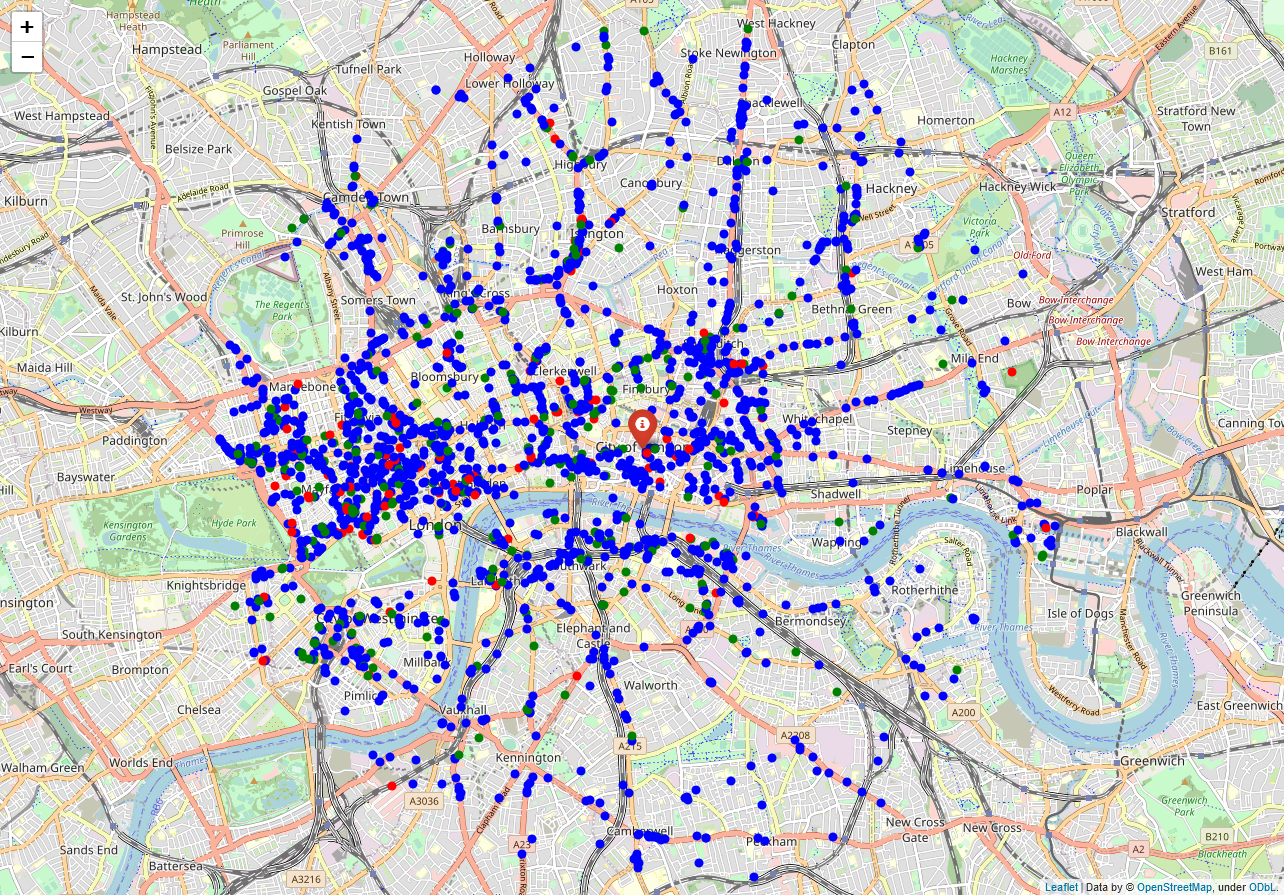
\includegraphics{08_restaurants}\end{center}

            % \begin{tcolorbox}[breakable, size=fbox, boxrule=.5pt, pad at break*=1mm, opacityfill=0]
% % \prompt{Out}{outcolor}{65}{\boxspacing}
% \begin{Verbatim}[commandchars=\\\{\}]
% <folium.folium.Map at 0x221e76b6850>
% \end{Verbatim}
% \end{tcolorbox}
        
    % \begin{tcolorbox}[breakable, size=fbox, boxrule=1pt, pad at break*=1mm,colback=cellbackground, colframe=cellborder]
% \prompt{In}{incolor}{66}{\boxspacing}
% \begin{Verbatim}[commandchars=\\\{\}]
% \PY{n}{save\PYZus{}map}\PY{p}{(}\PY{n}{map\PYZus{}city\PYZus{}resto}\PY{p}{,} \PY{l+s+s1}{\PYZsq{}}\PY{l+s+s1}{08\PYZus{}restaurants}\PY{l+s+s1}{\PYZsq{}}\PY{p}{)}
% \end{Verbatim}
% \end{tcolorbox}

    % \begin{Verbatim}[commandchars=\\\{\}]
% Map saved under '08\_restaurants.html' and '08\_restaurants.png'
    % \end{Verbatim}

    Looking good. We now have every restaurants around the City of London,
and we now which ones are either \textbf{Italian} or \textbf{French}.

We can move on to the analysis, and find our conclusions.

%    \begin{center}\rule{0.5\linewidth}{0.5pt}\end{center}

    \hypertarget{methodology}{%
\section{\texorpdfstring{Methodology
}{Methodology }}\label{methodology}}

In this project, we will first determine which type of restaurants are
the most prevalent: \textbf{Italian}, or \textbf{French}.

Then, for the less prevalent of the two, we will find areas around
London City that have a low restaurant density, and with particularly
low number of this type of restaurant. We will limit our analysis to a
radius of 5km.

The first step was to collect and process our data, which we did. We now
have usable areas, alongside their restaurants, and restaurants types.

The second step will consist in finding the density. We will use
\textbf{heatmaps} to locate the best areas, and focus our attention to
these.

In the last step, we will focus on the best areas, and create
\textbf{clusters} that meet the requierements. We will take locations
with \textbf{no more than two restaurants in a radius of 250 meters},
without \textbf{Italian (\emph{french})} restaurants in a radius of
400m, and no \textbf{French (\emph{italian})} restaurants in a radius of
250m.

We will present those areas on maps, and create clusters using
\textbf{k-means clustering} to identify the global zone that should be
considered.

%    \begin{center}\rule{0.5\linewidth}{0.5pt}\end{center}

    \hypertarget{analysis}{%
\section{\texorpdfstring{Analysis }{Analysis }}\label{analysis}}

Let's perform some basic explanatory data analysis and derive some
additional info from our raw data. First let's count the \textbf{number
of restaurants in every area candidate}:

    % \begin{tcolorbox}[breakable, size=fbox, boxrule=1pt, pad at break*=1mm,colback=cellbackground, colframe=cellborder]
% \prompt{In}{incolor}{67}{\boxspacing}
% \begin{Verbatim}[commandchars=\\\{\}]
% \PY{n}{location\PYZus{}restaurants\PYZus{}count} \PY{o}{=} \PY{p}{[}\PY{n+nb}{len}\PY{p}{(}\PY{n}{res}\PY{p}{)} \PY{k}{for} \PY{n}{res} \PY{o+ow}{in} \PY{n}{location\PYZus{}restaurants}\PY{p}{]}

% \PY{n}{hexa}\PY{p}{[}\PY{l+s+s1}{\PYZsq{}}\PY{l+s+s1}{Restaurants in area}\PY{l+s+s1}{\PYZsq{}}\PY{p}{]} \PY{o}{=} \PY{n}{location\PYZus{}restaurants\PYZus{}count}

% \PY{n+nb}{print}\PY{p}{(}\PY{l+s+s1}{\PYZsq{}}\PY{l+s+s1}{Average number of restaurants in every area with radius=250m:}\PY{l+s+s1}{\PYZsq{}}\PY{p}{,} \PY{n}{np}\PY{o}{.}\PY{n}{array}\PY{p}{(}\PY{n}{location\PYZus{}restaurants\PYZus{}count}\PY{p}{)}\PY{o}{.}\PY{n}{mean}\PY{p}{(}\PY{p}{)}\PY{p}{)}

% \PY{n}{hexa}\PY{o}{.}\PY{n}{head}\PY{p}{(}\PY{l+m+mi}{10}\PY{p}{)}
% \end{Verbatim}
% \end{tcolorbox}

\resizebox{\textwidth}{!}{%
    \begin{tabular}{lllllll}
    Average number of restaurants in every area with radius=250m: 5.44
    \\ \hline
    Address &
    Latitudes & Longitude &
    Distance from Center & X & Y &
    Restaurants in area
    \\ \hline
    Lambeth day nursery, Stockwell Park Road, Stoc{\ldots} &
    51.473259 & -0.116492 &
    4993.746089 & 700250.415693 & 5.706399e+06 & 0
    \\
    Dundas Road, Kennington, London Borough of Lam{\ldots} &
    51.473082 & -0.109302 &
    4866.980583 & 700750.415693 & 5.706399e+06 & 1
    \\
    2-4, Welby Street, Paulet Road Estate, Kenning{\ldots} &
    51.472904 & -0.102112 &
    4789.311015 & 701250.415693 & 5.706399e+06 & 1
    \\
    40, Valmar Road, Camberwell, London Borough of{\ldots} &
    51.472726 & -0.094922 &
    4763.139721 & 701750.415693 & 5.706399e+06 & 7
    \\
    4-8, Ribbon Dance Mews, Camberwell, London Bor{\ldots} &
    51.472548 & -0.087733 &
    4789.311015 & 702250.415693 & 5.706399e+06 & 9
    \\
    39, Shenley Road, Peckham, London Borough of S{\ldots} &
    51.472369 & -0.080543 &
    4866.980583 & 702750.415693 & 5.706399e+06 & 4
    \\
    Harris Academy at Peckham, 112, Peckham Road, {\ldots} &
    51.472189 & -0.073354 &
    4993.746089 & 703250.415693 & 5.706399e+06 & 1
    \\
    Hartington Road, Vauxhall, London Borough of L{\ldots} &
    51.477413 & -0.127033 &
    4879.805324 & 699500.415693 & 5.706832e+06 & 1
    \\
    20, Albert Square, Kennington, London Borough {\ldots} &
    51.477236 & -0.119842 &
    4670.385423 & 700000.415693 & 5.706832e+06 & 1
    \\
    Tesco Brixton Road, Caldwell Street, Kenningto{\ldots} &
    51.477059 & -0.112651 &
    4506.939094 & 700500.415693 & 5.706832e+06 & 2
    \end{tabular}
}

    % \begin{Verbatim}[commandchars=\\\{\}]
% Average number of restaurants in every area with radius=300m: 5.44
    % \end{Verbatim}

            % \begin{tcolorbox}[breakable, size=fbox, boxrule=.5pt, pad at break*=1mm, opacityfill=0]
% % \prompt{Out}{outcolor}{67}{\boxspacing}
% \begin{Verbatim}[commandchars=\\\{\}]
                                             % Address   Latitude  Longitude  \textbackslash{}
% 0  Lambeth day nursery, Stockwell Park Road, Stoc{\ldots}  51.473259  -0.116492
% 1  Dundas Road, Kennington, London Borough of Lam{\ldots}  51.473082  -0.109302
% 2  2-4, Welby Street, Paulet Road Estate, Kenning{\ldots}  51.472904  -0.102112
% 3  40, Valmar Road, Camberwell, London Borough of{\ldots}  51.472726  -0.094922
% 4  4-8, Ribbon Dance Mews, Camberwell, London Bor{\ldots}  51.472548  -0.087733
% 5  39, Shenley Road, Peckham, London Borough of S{\ldots}  51.472369  -0.080543
% 6  Harris Academy at Peckham, 112, Peckham Road, {\ldots}  51.472189  -0.073354
% 7  Hartington Road, Vauxhall, London Borough of L{\ldots}  51.477413  -0.127033
% 8  20, Albert Square, Kennington, London Borough {\ldots}  51.477236  -0.119842
% 9  Tesco Brixton Road, Caldwell Street, Kenningto{\ldots}  51.477059  -0.112651

   % Distance from Center              X             Y  Restaurants in area
% 0           4993.746089  700250.415693  5.706399e+06                    0
% 1           4866.980583  700750.415693  5.706399e+06                    1
% 2           4789.311015  701250.415693  5.706399e+06                    1
% 3           4763.139721  701750.415693  5.706399e+06                    7
% 4           4789.311015  702250.415693  5.706399e+06                    9
% 5           4866.980583  702750.415693  5.706399e+06                    4
% 6           4993.746089  703250.415693  5.706399e+06                    1
% 7           4879.805324  699500.415693  5.706832e+06                    1
% 8           4670.385423  700000.415693  5.706832e+06                    1
% 9           4506.939094  700500.415693  5.706832e+06                    2
% \end{Verbatim}
% \end{tcolorbox}
        
    OK, now let's calculate the \textbf{distance to nearest Italian and
French restaurant from every area candidate center} (not only those
within 250m - we want distance to closest one, regardless of how distant
it is):

    % \begin{tcolorbox}[breakable, size=fbox, boxrule=1pt, pad at break*=1mm,colback=cellbackground, colframe=cellborder]
% \prompt{In}{incolor}{110}{\boxspacing}
% \begin{Verbatim}[commandchars=\\\{\}]
% \PY{n}{distances\PYZus{}to\PYZus{}italian\PYZus{}restaurant} \PY{o}{=} \PY{p}{[}\PY{p}{]}
% \PY{n}{distances\PYZus{}to\PYZus{}french\PYZus{}restaurant} \PY{o}{=} \PY{p}{[}\PY{p}{]}

% \PY{k}{for} \PY{n}{area\PYZus{}x}\PY{p}{,} \PY{n}{area\PYZus{}y} \PY{o+ow}{in} \PY{n+nb}{zip}\PY{p}{(}\PY{n}{hexa}\PY{p}{[}\PY{l+s+s1}{\PYZsq{}}\PY{l+s+s1}{X}\PY{l+s+s1}{\PYZsq{}}\PY{p}{]}\PY{p}{,} \PY{n}{hexa}\PY{p}{[}\PY{l+s+s1}{\PYZsq{}}\PY{l+s+s1}{Y}\PY{l+s+s1}{\PYZsq{}}\PY{p}{]}\PY{p}{)}\PY{p}{:}
    % \PY{c+c1}{\PYZsh{} Italian}
    % \PY{n}{min\PYZus{}distance} \PY{o}{=} \PY{l+m+mi}{10000}
    % \PY{k}{for} \PY{n}{res} \PY{o+ow}{in} \PY{n}{italian\PYZus{}restaurants}\PY{o}{.}\PY{n}{values}\PY{p}{(}\PY{p}{)}\PY{p}{:}
        % \PY{n}{res\PYZus{}x} \PY{o}{=} \PY{n}{res}\PY{p}{[}\PY{l+m+mi}{8}\PY{p}{]}
        % \PY{n}{res\PYZus{}y} \PY{o}{=} \PY{n}{res}\PY{p}{[}\PY{l+m+mi}{9}\PY{p}{]}
        % \PY{n}{d} \PY{o}{=} \PY{n}{calc\PYZus{}xy\PYZus{}distance}\PY{p}{(}\PY{n}{area\PYZus{}x}\PY{p}{,} \PY{n}{area\PYZus{}y}\PY{p}{,} \PY{n}{res\PYZus{}x}\PY{p}{,} \PY{n}{res\PYZus{}y}\PY{p}{)}
        % \PY{k}{if} \PY{n}{d}\PY{o}{\PYZlt{}}\PY{n}{min\PYZus{}distance}\PY{p}{:}
            % \PY{n}{min\PYZus{}distance} \PY{o}{=} \PY{n}{d}
    % \PY{n}{distances\PYZus{}to\PYZus{}italian\PYZus{}restaurant}\PY{o}{.}\PY{n}{append}\PY{p}{(}\PY{n}{min\PYZus{}distance}\PY{p}{)}
    % \PY{c+c1}{\PYZsh{} French}
    % \PY{n}{min\PYZus{}distance} \PY{o}{=} \PY{l+m+mi}{10000}
    % \PY{k}{for} \PY{n}{res} \PY{o+ow}{in} \PY{n}{french\PYZus{}restaurants}\PY{o}{.}\PY{n}{values}\PY{p}{(}\PY{p}{)}\PY{p}{:}
        % \PY{n}{res\PYZus{}x} \PY{o}{=} \PY{n}{res}\PY{p}{[}\PY{l+m+mi}{8}\PY{p}{]}
        % \PY{n}{res\PYZus{}y} \PY{o}{=} \PY{n}{res}\PY{p}{[}\PY{l+m+mi}{9}\PY{p}{]}
        % \PY{n}{d} \PY{o}{=} \PY{n}{calc\PYZus{}xy\PYZus{}distance}\PY{p}{(}\PY{n}{area\PYZus{}x}\PY{p}{,} \PY{n}{area\PYZus{}y}\PY{p}{,} \PY{n}{res\PYZus{}x}\PY{p}{,} \PY{n}{res\PYZus{}y}\PY{p}{)}
        % \PY{k}{if} \PY{n}{d}\PY{o}{\PYZlt{}}\PY{n}{min\PYZus{}distance}\PY{p}{:}
            % \PY{n}{min\PYZus{}distance} \PY{o}{=} \PY{n}{d}
    % \PY{n}{distances\PYZus{}to\PYZus{}french\PYZus{}restaurant}\PY{o}{.}\PY{n}{append}\PY{p}{(}\PY{n}{min\PYZus{}distance}\PY{p}{)}

% \PY{n}{hexa}\PY{p}{[}\PY{l+s+s1}{\PYZsq{}}\PY{l+s+s1}{Distance to Italian restaurant}\PY{l+s+s1}{\PYZsq{}}\PY{p}{]} \PY{o}{=} \PY{n}{distances\PYZus{}to\PYZus{}italian\PYZus{}restaurant}
% \PY{n}{hexa}\PY{p}{[}\PY{l+s+s1}{\PYZsq{}}\PY{l+s+s1}{Distance to French restaurant}\PY{l+s+s1}{\PYZsq{}}\PY{p}{]} \PY{o}{=} \PY{n}{distances\PYZus{}to\PYZus{}french\PYZus{}restaurant}
% \end{Verbatim}
% \end{tcolorbox}

    % \begin{tcolorbox}[breakable, size=fbox, boxrule=1pt, pad at break*=1mm,colback=cellbackground, colframe=cellborder]
% \prompt{In}{incolor}{111}{\boxspacing}
% \begin{Verbatim}[commandchars=\\\{\}]
% \PY{n}{hexa}\PY{o}{.}\PY{n}{head}\PY{p}{(}\PY{l+m+mi}{10}\PY{p}{)}
% \end{Verbatim}
% \end{tcolorbox}

\resizebox{\textwidth}{!}{%
    \begin{tabular}{lllllllll}
    Address &
    Latitudes & Longitude &
    Distance from Center & X & Y & Restaurants in area &
    Distance to Italian restaurant &
    Distance to French restaurant
    \\ \hline
    Lambeth day nursery, Stockwell Park Road, Stoc{\ldots} &
    51.473259 & -0.116492 &
    4993.746089 & 700250.415693 & 5.706399e+06 & 0 &
    1156.951781 &
    1463.490762
    \\
    Dundas Road, Kennington, London Borough of Lam{\ldots} &
    51.473082 & -0.109302 &
    4866.980583 & 700750.415693 & 5.706399e+06 & 1 &
    1387.391283 &
    1926.789888
    \\
    2-4, Welby Street, Paulet Road Estate, Kenning{\ldots} &
    51.472904 & -0.102112 &
    4789.311015 & 701250.415693 & 5.706399e+06 & 1 &
    891.923212 &
    2029.583724
    \\
    40, Valmar Road, Camberwell, London Borough of{\ldots} &
    51.472726 & -0.094922 &
    4763.139721 & 701750.415693 & 5.706399e+06 & 7 &
    407.675682 &
    2129.980681
    \\
    4-8, Ribbon Dance Mews, Camberwell, London Bor{\ldots} &
    51.472548 & -0.087733 &
    4789.311015 & 702250.415693 & 5.706399e+06 & 9 &
    192.020588 &
    2335.471111
    \\
    39, Shenley Road, Peckham, London Borough of S{\ldots} &
    51.472369 & -0.080543 &
    4866.980583 & 702750.415693 & 5.706399e+06 & 4 &
    638.392004 &
    2621.456259
    \\
    Harris Academy at Peckham, 112, Peckham Road, {\ldots} &
    51.472189 & -0.073354 &
    4993.746089 & 703250.415693 & 5.706399e+06 & 1 &
    1130.582503 &
    2964.732792
    \\
    Hartington Road, Vauxhall, London Borough of L{\ldots} &
    51.477413 & -0.127033 &
    4879.805324 & 699500.415693 & 5.706832e+06 & 1 &
    628.490442 &
    603.914257
    \\
    20, Albert Square, Kennington, London Borough {\ldots} &
    51.477236 & -0.119842 &
    4670.385423 & 700000.415693 & 5.706832e+06 & 1 &
    657.670108 &
    1088.772929
    \\
    Tesco Brixton Road, Caldwell Street, Kenningto{\ldots} &
    51.477059 & -0.112651 &
    4506.939094 & 700500.415693 & 5.706832e+06 & 2 &
    977.733564 &
    1583.079452
    \end{tabular}
}

            % \begin{tcolorbox}[breakable, size=fbox, boxrule=.5pt, pad at break*=1mm, opacityfill=0]
% % \prompt{Out}{outcolor}{111}{\boxspacing}
% \begin{Verbatim}[commandchars=\\\{\}]
                                             % Address   Latitude  Longitude  \textbackslash{}
% 0  Lambeth day nursery, Stockwell Park Road, Stoc{\ldots}  51.473259  -0.116492
% 1  Dundas Road, Kennington, London Borough of Lam{\ldots}  51.473082  -0.109302
% 2  2-4, Welby Street, Paulet Road Estate, Kenning{\ldots}  51.472904  -0.102112
% 3  40, Valmar Road, Camberwell, London Borough of{\ldots}  51.472726  -0.094922
% 4  4-8, Ribbon Dance Mews, Camberwell, London Bor{\ldots}  51.472548  -0.087733
% 5  39, Shenley Road, Peckham, London Borough of S{\ldots}  51.472369  -0.080543
% 6  Harris Academy at Peckham, 112, Peckham Road, {\ldots}  51.472189  -0.073354
% 7  Hartington Road, Vauxhall, London Borough of L{\ldots}  51.477413  -0.127033
% 8  20, Albert Square, Kennington, London Borough {\ldots}  51.477236  -0.119842
% 9  Tesco Brixton Road, Caldwell Street, Kenningto{\ldots}  51.477059  -0.112651

   % Distance from Center              X             Y  Restaurants in area  \textbackslash{}
% 0           4993.746089  700250.415693  5.706399e+06                    0
% 1           4866.980583  700750.415693  5.706399e+06                    1
% 2           4789.311015  701250.415693  5.706399e+06                    1
% 3           4763.139721  701750.415693  5.706399e+06                    7
% 4           4789.311015  702250.415693  5.706399e+06                    9
% 5           4866.980583  702750.415693  5.706399e+06                    4
% 6           4993.746089  703250.415693  5.706399e+06                    1
% 7           4879.805324  699500.415693  5.706832e+06                    1
% 8           4670.385423  700000.415693  5.706832e+06                    1
% 9           4506.939094  700500.415693  5.706832e+06                    2

   % Distance to Italian restaurant  Distance to French restaurant
% 0                     1156.951781                    1463.490762
% 1                     1387.391283                    1926.789888
% 2                      891.923212                    2029.583724
% 3                      407.675682                    2129.980681
% 4                      192.020588                    2335.471111
% 5                      638.392004                    2621.456259
% 6                     1130.582503                    2964.732792
% 7                      628.490442                     603.914257
% 8                      657.670108                    1088.772929
% 9                      977.733564                    1583.079452
% \end{Verbatim}
% \end{tcolorbox}
        
    % \begin{tcolorbox}[breakable, size=fbox, boxrule=1pt, pad at break*=1mm,colback=cellbackground, colframe=cellborder]
% \prompt{In}{incolor}{112}{\boxspacing}
% \begin{Verbatim}[commandchars=\\\{\}]
% \PY{n+nb}{print}\PY{p}{(}\PY{l+s+s1}{\PYZsq{}}\PY{l+s+s1}{Average distance to closest Italian restaurant from each area center:}\PY{l+s+s1}{\PYZsq{}}\PY{p}{,} \PY{n}{hexa}\PY{p}{[}\PY{l+s+s1}{\PYZsq{}}\PY{l+s+s1}{Distance to Italian restaurant}\PY{l+s+s1}{\PYZsq{}}\PY{p}{]}\PY{o}{.}\PY{n}{mean}\PY{p}{(}\PY{p}{)}\PY{p}{)}
% \PY{n+nb}{print}\PY{p}{(}\PY{l+s+s1}{\PYZsq{}}\PY{l+s+s1}{Average distance to closest French restaurant from each area center:}\PY{l+s+s1}{\PYZsq{}}\PY{p}{,} \PY{n}{hexa}\PY{p}{[}\PY{l+s+s1}{\PYZsq{}}\PY{l+s+s1}{Distance to French restaurant}\PY{l+s+s1}{\PYZsq{}}\PY{p}{]}\PY{o}{.}\PY{n}{mean}\PY{p}{(}\PY{p}{)}\PY{p}{)}
% \end{Verbatim}
% \end{tcolorbox}

    \begin{Verbatim}[commandchars=\\\{\}]
Average distance to closest Italian restaurant from each area center:
429.952222459347
Average distance to closest French restaurant from each area center:
900.1205600724
    \end{Verbatim}

    On average \textbf{Italian} restaurant can be found within
\textbf{\textasciitilde900m}, and a \textbf{French} within
\textbf{\textasciitilde430m} from every area center candidate.
Considering on how close it is, we need to focus on our areas more.

Let us note that it look like \textbf{French} restaurants are almost two
times less prevalent that \textbf{Italian} ones. Let's see if we can
confirm that.

Let's create a \textbf{heatmap} showing the density of restaurants, and
let's use our GeoJSON file to plot the boundaries of each boroughs. We
will also add circles around 1km, 2km, and 3km from the center:

    % \begin{tcolorbox}[breakable, size=fbox, boxrule=1pt, pad at break*=1mm,colback=cellbackground, colframe=cellborder]
% \prompt{In}{incolor}{71}{\boxspacing}
% \begin{Verbatim}[commandchars=\\\{\}]
% \PY{n}{london\PYZus{}boroughs\PYZus{}boundaries} \PY{o}{=} \PY{n}{requests}\PY{o}{.}\PY{n}{get}\PY{p}{(}\PY{n}{url\PYZus{}geolondon}\PY{p}{)}\PY{o}{.}\PY{n}{json}\PY{p}{(}\PY{p}{)}

% \PY{k}{def} \PY{n+nf}{boroughs\PYZus{}style}\PY{p}{(}\PY{n}{feature}\PY{p}{)}\PY{p}{:}
    % \PY{k}{return} \PY{p}{\PYZob{}} \PY{l+s+s1}{\PYZsq{}}\PY{l+s+s1}{color}\PY{l+s+s1}{\PYZsq{}}\PY{p}{:} \PY{l+s+s1}{\PYZsq{}}\PY{l+s+s1}{blue}\PY{l+s+s1}{\PYZsq{}}\PY{p}{,} \PY{l+s+s1}{\PYZsq{}}\PY{l+s+s1}{fill}\PY{l+s+s1}{\PYZsq{}}\PY{p}{:} \PY{k+kc}{False} \PY{p}{\PYZcb{}}

% \PY{n}{restaurant\PYZus{}latlong} \PY{o}{=} \PY{p}{[}\PY{p}{[}\PY{n}{res}\PY{p}{[}\PY{l+m+mi}{2}\PY{p}{]}\PY{p}{,} \PY{n}{res}\PY{p}{[}\PY{l+m+mi}{3}\PY{p}{]}\PY{p}{]} \PY{k}{for} \PY{n}{res} \PY{o+ow}{in} \PY{n}{restaurants}\PY{o}{.}\PY{n}{values}\PY{p}{(}\PY{p}{)}\PY{p}{]}

% \PY{n}{italian\PYZus{}latlong} \PY{o}{=} \PY{p}{[}\PY{p}{[}\PY{n}{res}\PY{p}{[}\PY{l+m+mi}{2}\PY{p}{]}\PY{p}{,} \PY{n}{res}\PY{p}{[}\PY{l+m+mi}{3}\PY{p}{]}\PY{p}{]} \PY{k}{for} \PY{n}{res} \PY{o+ow}{in} \PY{n}{italian\PYZus{}restaurants}\PY{o}{.}\PY{n}{values}\PY{p}{(}\PY{p}{)}\PY{p}{]}
% \PY{n}{french\PYZus{}latlong} \PY{o}{=} \PY{p}{[}\PY{p}{[}\PY{n}{res}\PY{p}{[}\PY{l+m+mi}{2}\PY{p}{]}\PY{p}{,} \PY{n}{res}\PY{p}{[}\PY{l+m+mi}{3}\PY{p}{]}\PY{p}{]} \PY{k}{for} \PY{n}{res} \PY{o+ow}{in} \PY{n}{french\PYZus{}restaurants}\PY{o}{.}\PY{n}{values}\PY{p}{(}\PY{p}{)}\PY{p}{]}
% \end{Verbatim}
% \end{tcolorbox}

    % \begin{tcolorbox}[breakable, size=fbox, boxrule=1pt, pad at break*=1mm,colback=cellbackground, colframe=cellborder]
% \prompt{In}{incolor}{72}{\boxspacing}
% \begin{Verbatim}[commandchars=\\\{\}]
% \PY{n}{map\PYZus{}rest\PYZus{}heat\PYZus{}all} \PY{o}{=} \PY{n}{folium}\PY{o}{.}\PY{n}{Map}\PY{p}{(}\PY{n}{location}\PY{o}{=}\PY{p}{[}\PY{n}{city\PYZus{}latitude}\PY{p}{,} \PY{n}{city\PYZus{}longitude}\PY{p}{]}\PY{p}{,} \PY{n}{zoom\PYZus{}start}\PY{o}{=}\PY{l+m+mi}{13}\PY{p}{)}
% \PY{n}{folium}\PY{o}{.}\PY{n}{TileLayer}\PY{p}{(}\PY{l+s+s1}{\PYZsq{}}\PY{l+s+s1}{cartodbpositron}\PY{l+s+s1}{\PYZsq{}}\PY{p}{)}\PY{o}{.}\PY{n}{add\PYZus{}to}\PY{p}{(}\PY{n}{map\PYZus{}rest\PYZus{}heat\PYZus{}all}\PY{p}{)} \PY{c+c1}{\PYZsh{}cartodbpositron cartodbdark\PYZus{}matter}
% \PY{n}{HeatMap}\PY{p}{(}\PY{n}{restaurant\PYZus{}latlong}\PY{p}{)}\PY{o}{.}\PY{n}{add\PYZus{}to}\PY{p}{(}\PY{n}{map\PYZus{}rest\PYZus{}heat\PYZus{}all}\PY{p}{)}
% \PY{n}{folium}\PY{o}{.}\PY{n}{Marker}\PY{p}{(}\PY{p}{[}\PY{n}{city\PYZus{}latitude}\PY{p}{,} \PY{n}{city\PYZus{}longitude}\PY{p}{]}\PY{p}{,} \PY{n}{icon}\PY{o}{=}\PY{n}{folium}\PY{o}{.}\PY{n}{Icon}\PY{p}{(}\PY{n}{color}\PY{o}{=}\PY{l+s+s1}{\PYZsq{}}\PY{l+s+s1}{red}\PY{l+s+s1}{\PYZsq{}}\PY{p}{,} \PY{n}{icon}\PY{o}{=}\PY{l+s+s1}{\PYZsq{}}\PY{l+s+s1}{info\PYZhy{}sign}\PY{l+s+s1}{\PYZsq{}}\PY{p}{)}\PY{p}{,} \PY{n}{popup}\PY{o}{=}\PY{l+s+s1}{\PYZsq{}}\PY{l+s+s1}{City Center}\PY{l+s+s1}{\PYZsq{}}\PY{p}{)}\PY{o}{.}\PY{n}{add\PYZus{}to}\PY{p}{(}\PY{n}{map\PYZus{}rest\PYZus{}heat\PYZus{}all}\PY{p}{)}
% \PY{n}{folium}\PY{o}{.}\PY{n}{Circle}\PY{p}{(}\PY{p}{[}\PY{n}{city\PYZus{}latitude}\PY{p}{,} \PY{n}{city\PYZus{}longitude}\PY{p}{]}\PY{p}{,} \PY{n}{radius}\PY{o}{=}\PY{l+m+mi}{1000}\PY{p}{,} \PY{n}{fill}\PY{o}{=}\PY{k+kc}{False}\PY{p}{,} \PY{n}{color}\PY{o}{=}\PY{l+s+s1}{\PYZsq{}}\PY{l+s+s1}{white}\PY{l+s+s1}{\PYZsq{}}\PY{p}{)}\PY{o}{.}\PY{n}{add\PYZus{}to}\PY{p}{(}\PY{n}{map\PYZus{}rest\PYZus{}heat\PYZus{}all}\PY{p}{)}
% \PY{n}{folium}\PY{o}{.}\PY{n}{Circle}\PY{p}{(}\PY{p}{[}\PY{n}{city\PYZus{}latitude}\PY{p}{,} \PY{n}{city\PYZus{}longitude}\PY{p}{]}\PY{p}{,} \PY{n}{radius}\PY{o}{=}\PY{l+m+mi}{2000}\PY{p}{,} \PY{n}{fill}\PY{o}{=}\PY{k+kc}{False}\PY{p}{,} \PY{n}{color}\PY{o}{=}\PY{l+s+s1}{\PYZsq{}}\PY{l+s+s1}{white}\PY{l+s+s1}{\PYZsq{}}\PY{p}{)}\PY{o}{.}\PY{n}{add\PYZus{}to}\PY{p}{(}\PY{n}{map\PYZus{}rest\PYZus{}heat\PYZus{}all}\PY{p}{)}
% \PY{n}{folium}\PY{o}{.}\PY{n}{Circle}\PY{p}{(}\PY{p}{[}\PY{n}{city\PYZus{}latitude}\PY{p}{,} \PY{n}{city\PYZus{}longitude}\PY{p}{]}\PY{p}{,} \PY{n}{radius}\PY{o}{=}\PY{l+m+mi}{3000}\PY{p}{,} \PY{n}{fill}\PY{o}{=}\PY{k+kc}{False}\PY{p}{,} \PY{n}{color}\PY{o}{=}\PY{l+s+s1}{\PYZsq{}}\PY{l+s+s1}{white}\PY{l+s+s1}{\PYZsq{}}\PY{p}{)}\PY{o}{.}\PY{n}{add\PYZus{}to}\PY{p}{(}\PY{n}{map\PYZus{}rest\PYZus{}heat\PYZus{}all}\PY{p}{)}
% \PY{n}{folium}\PY{o}{.}\PY{n}{GeoJson}\PY{p}{(}\PY{n}{london\PYZus{}boroughs\PYZus{}boundaries}\PY{p}{,} \PY{n}{style\PYZus{}function}\PY{o}{=}\PY{n}{boroughs\PYZus{}style}\PY{p}{,} \PY{n}{name}\PY{o}{=}\PY{l+s+s1}{\PYZsq{}}\PY{l+s+s1}{geojson}\PY{l+s+s1}{\PYZsq{}}\PY{p}{)}\PY{o}{.}\PY{n}{add\PYZus{}to}\PY{p}{(}\PY{n}{map\PYZus{}rest\PYZus{}heat\PYZus{}all}\PY{p}{)}

% \PY{c+c1}{\PYZsh{} Add markers corresponding to the neighborhoods to the map}
% \PY{k}{for} \PY{n}{lat}\PY{p}{,} \PY{n}{lng}\PY{p}{,} \PY{n}{borough}\PY{p}{,} \PY{n}{neighborhood} \PY{o+ow}{in} \PY{n+nb}{zip}\PY{p}{(}\PY{n}{neigh\PYZus{}data}\PY{p}{[}\PY{l+s+s1}{\PYZsq{}}\PY{l+s+s1}{Latitude}\PY{l+s+s1}{\PYZsq{}}\PY{p}{]}\PY{p}{,} \PY{n}{neigh\PYZus{}data}\PY{p}{[}\PY{l+s+s1}{\PYZsq{}}\PY{l+s+s1}{Longitude}\PY{l+s+s1}{\PYZsq{}}\PY{p}{]}\PY{p}{,} \PY{n}{neigh\PYZus{}data}\PY{p}{[}\PY{l+s+s1}{\PYZsq{}}\PY{l+s+s1}{Borough}\PY{l+s+s1}{\PYZsq{}}\PY{p}{]}\PY{p}{,} \PY{n}{neigh\PYZus{}data}\PY{p}{[}\PY{l+s+s1}{\PYZsq{}}\PY{l+s+s1}{Neighborhood}\PY{l+s+s1}{\PYZsq{}}\PY{p}{]}\PY{p}{)}\PY{p}{:}
    % \PY{n}{label} \PY{o}{=} \PY{l+s+s1}{\PYZsq{}}\PY{l+s+si}{\PYZob{}\PYZcb{}}\PY{l+s+s1}{, }\PY{l+s+si}{\PYZob{}\PYZcb{}}\PY{l+s+s1}{\PYZsq{}}\PY{o}{.}\PY{n}{format}\PY{p}{(}\PY{n}{neighborhood}\PY{p}{,} \PY{n}{borough}\PY{p}{)}
    % \PY{n}{label} \PY{o}{=} \PY{n}{folium}\PY{o}{.}\PY{n}{Popup}\PY{p}{(}\PY{n}{label}\PY{p}{,} \PY{n}{parse\PYZus{}html}\PY{o}{=}\PY{k+kc}{True}\PY{p}{)}
    % \PY{n}{folium}\PY{o}{.}\PY{n}{CircleMarker}\PY{p}{(}
        % \PY{p}{[}\PY{n}{lat}\PY{p}{,} \PY{n}{lng}\PY{p}{]}\PY{p}{,}
        % \PY{n}{radius}\PY{o}{=}\PY{l+m+mi}{5}\PY{p}{,}
        % \PY{n}{popup}\PY{o}{=}\PY{n}{label}\PY{p}{,}
        % \PY{n}{color}\PY{o}{=}\PY{l+s+s1}{\PYZsq{}}\PY{l+s+s1}{green}\PY{l+s+s1}{\PYZsq{}}\PY{p}{,}
        % \PY{n}{fill}\PY{o}{=}\PY{k+kc}{True}\PY{p}{,}
        % \PY{n}{fill\PYZus{}color}\PY{o}{=}\PY{l+s+s1}{\PYZsq{}}\PY{l+s+s1}{\PYZsh{}3186cc}\PY{l+s+s1}{\PYZsq{}}\PY{p}{,}
        % \PY{n}{fill\PYZus{}opacity}\PY{o}{=}\PY{l+m+mf}{0.7}\PY{p}{,}
        % \PY{n}{parse\PYZus{}html}\PY{o}{=}\PY{k+kc}{False}\PY{p}{)}\PY{o}{.}\PY{n}{add\PYZus{}to}\PY{p}{(}\PY{n}{map\PYZus{}rest\PYZus{}heat\PYZus{}all}\PY{p}{)}  

% \PY{n}{map\PYZus{}rest\PYZus{}heat\PYZus{}all}
% \end{Verbatim}
% \end{tcolorbox}

\begin{center}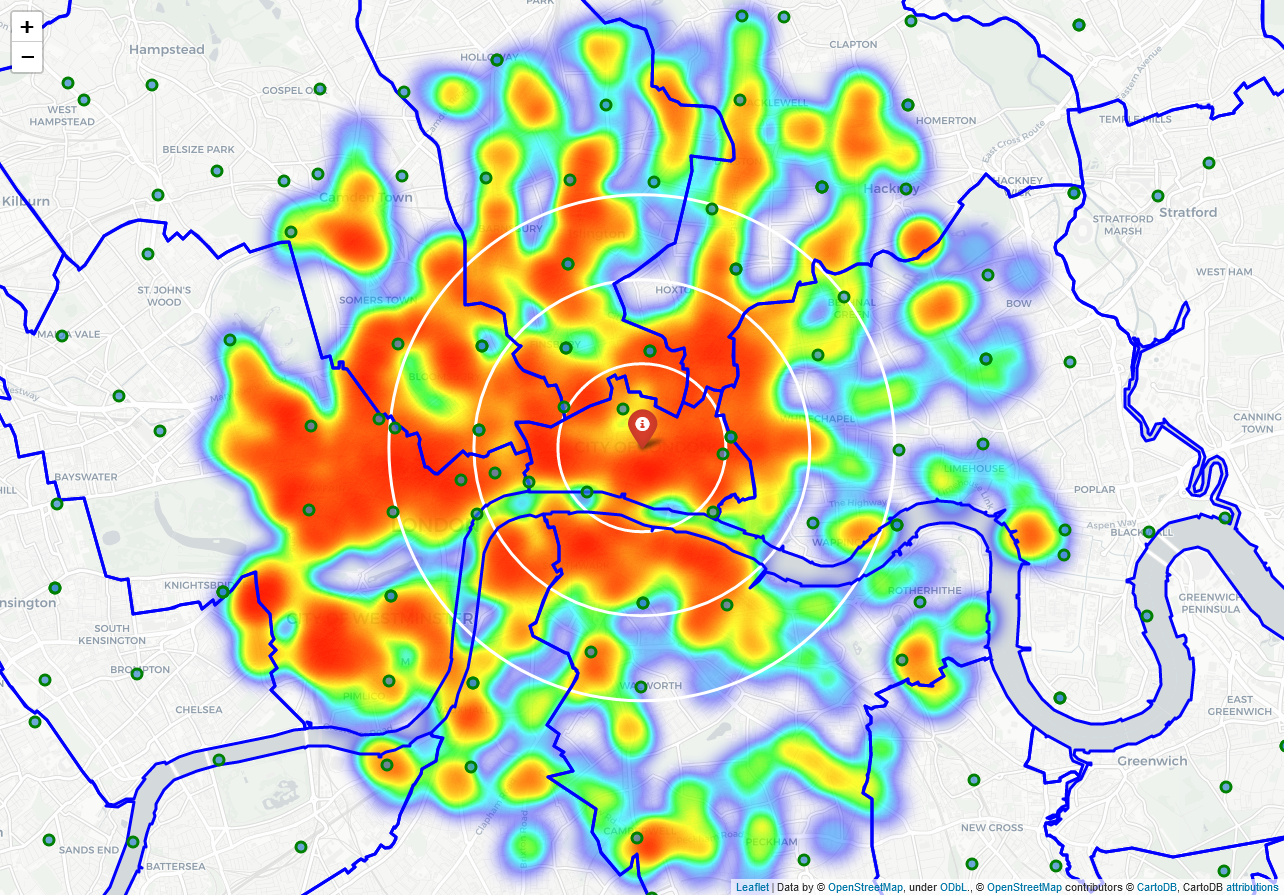
\includegraphics{09_rest_heat_all}\end{center}

            % \begin{tcolorbox}[breakable, size=fbox, boxrule=.5pt, pad at break*=1mm, opacityfill=0]
% % \prompt{Out}{outcolor}{72}{\boxspacing}
% \begin{Verbatim}[commandchars=\\\{\}]
% <folium.folium.Map at 0x221ec15e190>
% \end{Verbatim}
% \end{tcolorbox}
        
    % \begin{tcolorbox}[breakable, size=fbox, boxrule=1pt, pad at break*=1mm,colback=cellbackground, colframe=cellborder]
% \prompt{In}{incolor}{73}{\boxspacing}
% \begin{Verbatim}[commandchars=\\\{\}]
% \PY{n}{save\PYZus{}map}\PY{p}{(}\PY{n}{map\PYZus{}rest\PYZus{}heat\PYZus{}all}\PY{p}{,} \PY{l+s+s1}{\PYZsq{}}\PY{l+s+s1}{09\PYZus{}rest\PYZus{}heat\PYZus{}all}\PY{l+s+s1}{\PYZsq{}}\PY{p}{)}
% \end{Verbatim}
% \end{tcolorbox}

    % \begin{Verbatim}[commandchars=\\\{\}]
% Map saved under '09\_rest\_heat\_all.html' and '09\_rest\_heat\_all.png'
    % \end{Verbatim}

    Looks like a most restaurants are located on the western part of the
city.

Let's create another heatmap map showing only the \textbf{Italian}
restaurants:

    % \begin{tcolorbox}[breakable, size=fbox, boxrule=1pt, pad at break*=1mm,colback=cellbackground, colframe=cellborder]
% \prompt{In}{incolor}{74}{\boxspacing}
% \begin{Verbatim}[commandchars=\\\{\}]
% \PY{n}{map\PYZus{}rest\PYZus{}heat\PYZus{}ita} \PY{o}{=} \PY{n}{folium}\PY{o}{.}\PY{n}{Map}\PY{p}{(}\PY{n}{location}\PY{o}{=}\PY{p}{[}\PY{n}{city\PYZus{}latitude}\PY{p}{,} \PY{n}{city\PYZus{}longitude}\PY{p}{]}\PY{p}{,} \PY{n}{zoom\PYZus{}start}\PY{o}{=}\PY{l+m+mi}{13}\PY{p}{)}
% \PY{n}{folium}\PY{o}{.}\PY{n}{TileLayer}\PY{p}{(}\PY{l+s+s1}{\PYZsq{}}\PY{l+s+s1}{cartodbpositron}\PY{l+s+s1}{\PYZsq{}}\PY{p}{)}\PY{o}{.}\PY{n}{add\PYZus{}to}\PY{p}{(}\PY{n}{map\PYZus{}rest\PYZus{}heat\PYZus{}ita}\PY{p}{)} \PY{c+c1}{\PYZsh{}cartodbpositron cartodbdark\PYZus{}matter}
% \PY{n}{HeatMap}\PY{p}{(}\PY{n}{italian\PYZus{}latlong}\PY{p}{)}\PY{o}{.}\PY{n}{add\PYZus{}to}\PY{p}{(}\PY{n}{map\PYZus{}rest\PYZus{}heat\PYZus{}ita}\PY{p}{)}
% \PY{n}{folium}\PY{o}{.}\PY{n}{Marker}\PY{p}{(}\PY{p}{[}\PY{n}{city\PYZus{}latitude}\PY{p}{,} \PY{n}{city\PYZus{}longitude}\PY{p}{]}\PY{p}{,} \PY{n}{icon}\PY{o}{=}\PY{n}{folium}\PY{o}{.}\PY{n}{Icon}\PY{p}{(}\PY{n}{color}\PY{o}{=}\PY{l+s+s1}{\PYZsq{}}\PY{l+s+s1}{red}\PY{l+s+s1}{\PYZsq{}}\PY{p}{,} \PY{n}{icon}\PY{o}{=}\PY{l+s+s1}{\PYZsq{}}\PY{l+s+s1}{info\PYZhy{}sign}\PY{l+s+s1}{\PYZsq{}}\PY{p}{)}\PY{p}{,} \PY{n}{popup}\PY{o}{=}\PY{l+s+s1}{\PYZsq{}}\PY{l+s+s1}{City Center}\PY{l+s+s1}{\PYZsq{}}\PY{p}{)}\PY{o}{.}\PY{n}{add\PYZus{}to}\PY{p}{(}\PY{n}{map\PYZus{}rest\PYZus{}heat\PYZus{}ita}\PY{p}{)}
% \PY{n}{folium}\PY{o}{.}\PY{n}{Circle}\PY{p}{(}\PY{p}{[}\PY{n}{city\PYZus{}latitude}\PY{p}{,} \PY{n}{city\PYZus{}longitude}\PY{p}{]}\PY{p}{,} \PY{n}{radius}\PY{o}{=}\PY{l+m+mi}{1000}\PY{p}{,} \PY{n}{fill}\PY{o}{=}\PY{k+kc}{False}\PY{p}{,} \PY{n}{color}\PY{o}{=}\PY{l+s+s1}{\PYZsq{}}\PY{l+s+s1}{white}\PY{l+s+s1}{\PYZsq{}}\PY{p}{)}\PY{o}{.}\PY{n}{add\PYZus{}to}\PY{p}{(}\PY{n}{map\PYZus{}rest\PYZus{}heat\PYZus{}ita}\PY{p}{)}
% \PY{n}{folium}\PY{o}{.}\PY{n}{Circle}\PY{p}{(}\PY{p}{[}\PY{n}{city\PYZus{}latitude}\PY{p}{,} \PY{n}{city\PYZus{}longitude}\PY{p}{]}\PY{p}{,} \PY{n}{radius}\PY{o}{=}\PY{l+m+mi}{2000}\PY{p}{,} \PY{n}{fill}\PY{o}{=}\PY{k+kc}{False}\PY{p}{,} \PY{n}{color}\PY{o}{=}\PY{l+s+s1}{\PYZsq{}}\PY{l+s+s1}{white}\PY{l+s+s1}{\PYZsq{}}\PY{p}{)}\PY{o}{.}\PY{n}{add\PYZus{}to}\PY{p}{(}\PY{n}{map\PYZus{}rest\PYZus{}heat\PYZus{}ita}\PY{p}{)}
% \PY{n}{folium}\PY{o}{.}\PY{n}{Circle}\PY{p}{(}\PY{p}{[}\PY{n}{city\PYZus{}latitude}\PY{p}{,} \PY{n}{city\PYZus{}longitude}\PY{p}{]}\PY{p}{,} \PY{n}{radius}\PY{o}{=}\PY{l+m+mi}{3000}\PY{p}{,} \PY{n}{fill}\PY{o}{=}\PY{k+kc}{False}\PY{p}{,} \PY{n}{color}\PY{o}{=}\PY{l+s+s1}{\PYZsq{}}\PY{l+s+s1}{white}\PY{l+s+s1}{\PYZsq{}}\PY{p}{)}\PY{o}{.}\PY{n}{add\PYZus{}to}\PY{p}{(}\PY{n}{map\PYZus{}rest\PYZus{}heat\PYZus{}ita}\PY{p}{)}
% \PY{n}{folium}\PY{o}{.}\PY{n}{GeoJson}\PY{p}{(}\PY{n}{london\PYZus{}boroughs\PYZus{}boundaries}\PY{p}{,} \PY{n}{style\PYZus{}function}\PY{o}{=}\PY{n}{boroughs\PYZus{}style}\PY{p}{,} \PY{n}{name}\PY{o}{=}\PY{l+s+s1}{\PYZsq{}}\PY{l+s+s1}{geojson}\PY{l+s+s1}{\PYZsq{}}\PY{p}{)}\PY{o}{.}\PY{n}{add\PYZus{}to}\PY{p}{(}\PY{n}{map\PYZus{}rest\PYZus{}heat\PYZus{}ita}\PY{p}{)}

% \PY{c+c1}{\PYZsh{} Add markers corresponding to the neighborhoods to the map}
% \PY{k}{for} \PY{n}{lat}\PY{p}{,} \PY{n}{lng}\PY{p}{,} \PY{n}{borough}\PY{p}{,} \PY{n}{neighborhood} \PY{o+ow}{in} \PY{n+nb}{zip}\PY{p}{(}\PY{n}{neigh\PYZus{}data}\PY{p}{[}\PY{l+s+s1}{\PYZsq{}}\PY{l+s+s1}{Latitude}\PY{l+s+s1}{\PYZsq{}}\PY{p}{]}\PY{p}{,} \PY{n}{neigh\PYZus{}data}\PY{p}{[}\PY{l+s+s1}{\PYZsq{}}\PY{l+s+s1}{Longitude}\PY{l+s+s1}{\PYZsq{}}\PY{p}{]}\PY{p}{,} \PY{n}{neigh\PYZus{}data}\PY{p}{[}\PY{l+s+s1}{\PYZsq{}}\PY{l+s+s1}{Borough}\PY{l+s+s1}{\PYZsq{}}\PY{p}{]}\PY{p}{,} \PY{n}{neigh\PYZus{}data}\PY{p}{[}\PY{l+s+s1}{\PYZsq{}}\PY{l+s+s1}{Neighborhood}\PY{l+s+s1}{\PYZsq{}}\PY{p}{]}\PY{p}{)}\PY{p}{:}
    % \PY{n}{label} \PY{o}{=} \PY{l+s+s1}{\PYZsq{}}\PY{l+s+si}{\PYZob{}\PYZcb{}}\PY{l+s+s1}{, }\PY{l+s+si}{\PYZob{}\PYZcb{}}\PY{l+s+s1}{\PYZsq{}}\PY{o}{.}\PY{n}{format}\PY{p}{(}\PY{n}{neighborhood}\PY{p}{,} \PY{n}{borough}\PY{p}{)}
    % \PY{n}{label} \PY{o}{=} \PY{n}{folium}\PY{o}{.}\PY{n}{Popup}\PY{p}{(}\PY{n}{label}\PY{p}{,} \PY{n}{parse\PYZus{}html}\PY{o}{=}\PY{k+kc}{True}\PY{p}{)}
    % \PY{n}{folium}\PY{o}{.}\PY{n}{CircleMarker}\PY{p}{(}
        % \PY{p}{[}\PY{n}{lat}\PY{p}{,} \PY{n}{lng}\PY{p}{]}\PY{p}{,}
        % \PY{n}{radius}\PY{o}{=}\PY{l+m+mi}{5}\PY{p}{,}
        % \PY{n}{popup}\PY{o}{=}\PY{n}{label}\PY{p}{,}
        % \PY{n}{color}\PY{o}{=}\PY{l+s+s1}{\PYZsq{}}\PY{l+s+s1}{green}\PY{l+s+s1}{\PYZsq{}}\PY{p}{,}
        % \PY{n}{fill}\PY{o}{=}\PY{k+kc}{True}\PY{p}{,}
        % \PY{n}{fill\PYZus{}color}\PY{o}{=}\PY{l+s+s1}{\PYZsq{}}\PY{l+s+s1}{\PYZsh{}3186cc}\PY{l+s+s1}{\PYZsq{}}\PY{p}{,}
        % \PY{n}{fill\PYZus{}opacity}\PY{o}{=}\PY{l+m+mf}{0.7}\PY{p}{,}
        % \PY{n}{parse\PYZus{}html}\PY{o}{=}\PY{k+kc}{False}\PY{p}{)}\PY{o}{.}\PY{n}{add\PYZus{}to}\PY{p}{(}\PY{n}{map\PYZus{}rest\PYZus{}heat\PYZus{}ita}\PY{p}{)}  

% \PY{n}{map\PYZus{}rest\PYZus{}heat\PYZus{}ita}
% \end{Verbatim}
% \end{tcolorbox}

\begin{center}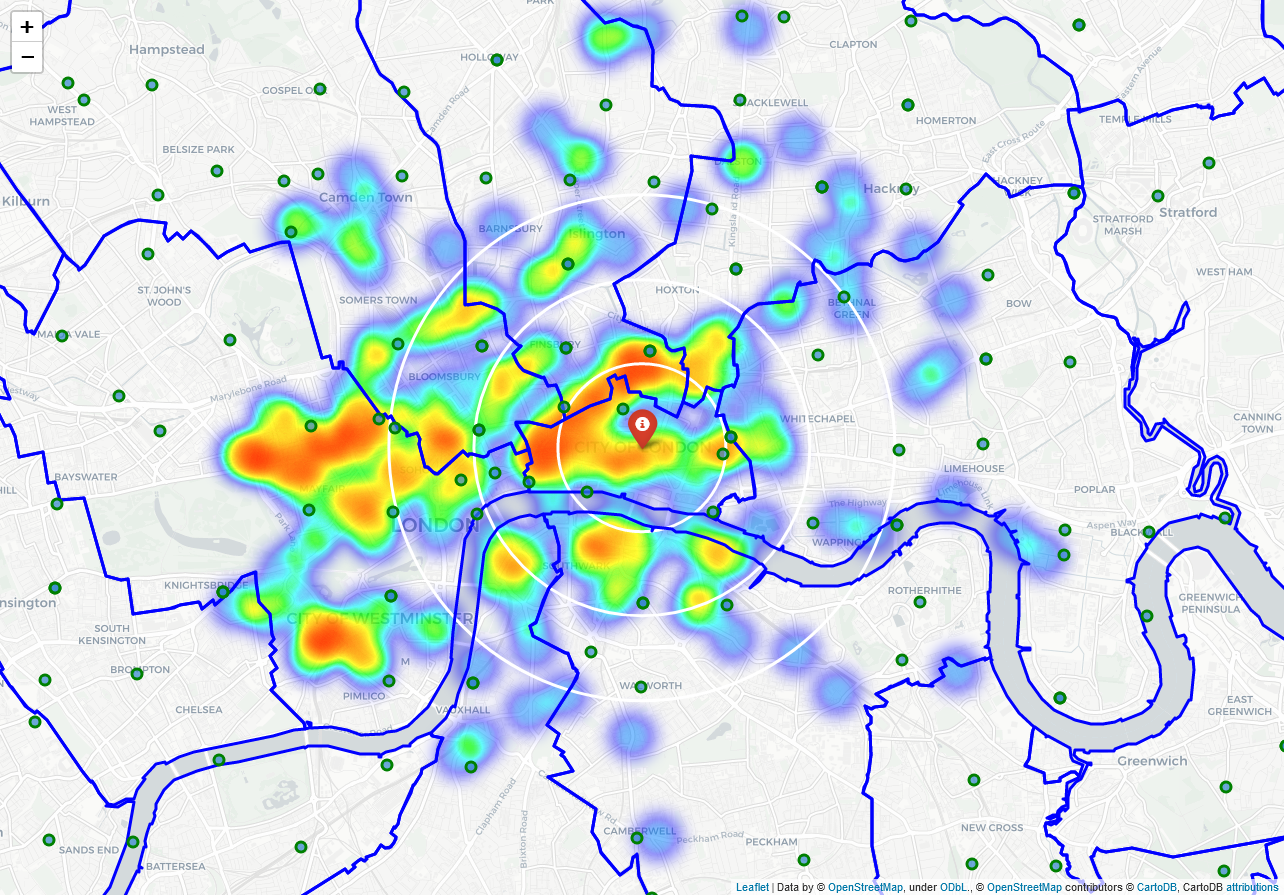
\includegraphics{10_rest_heat_ita}\end{center}

            % \begin{tcolorbox}[breakable, size=fbox, boxrule=.5pt, pad at break*=1mm, opacityfill=0]
% % \prompt{Out}{outcolor}{74}{\boxspacing}
% \begin{Verbatim}[commandchars=\\\{\}]
% <folium.folium.Map at 0x221ee69d700>
% \end{Verbatim}
% \end{tcolorbox}
        
    % \begin{tcolorbox}[breakable, size=fbox, boxrule=1pt, pad at break*=1mm,colback=cellbackground, colframe=cellborder]
% \prompt{In}{incolor}{75}{\boxspacing}
% \begin{Verbatim}[commandchars=\\\{\}]
% \PY{n}{save\PYZus{}map}\PY{p}{(}\PY{n}{map\PYZus{}rest\PYZus{}heat\PYZus{}ita}\PY{p}{,} \PY{l+s+s1}{\PYZsq{}}\PY{l+s+s1}{10\PYZus{}rest\PYZus{}heat\PYZus{}ita}\PY{l+s+s1}{\PYZsq{}}\PY{p}{)}
% \end{Verbatim}
% \end{tcolorbox}

    % \begin{Verbatim}[commandchars=\\\{\}]
% Map saved under '10\_rest\_heat\_ita.html' and '10\_rest\_heat\_ita.png'
    % \end{Verbatim}

    \textbf{Italians} restaurant are pretty present, and follow the same
areas density.

Let's have a look at the \textbf{French} ones:

    % \begin{tcolorbox}[breakable, size=fbox, boxrule=1pt, pad at break*=1mm,colback=cellbackground, colframe=cellborder]
% \prompt{In}{incolor}{76}{\boxspacing}
% \begin{Verbatim}[commandchars=\\\{\}]
% \PY{n}{map\PYZus{}rest\PYZus{}heat\PYZus{}fre} \PY{o}{=} \PY{n}{folium}\PY{o}{.}\PY{n}{Map}\PY{p}{(}\PY{n}{location}\PY{o}{=}\PY{p}{[}\PY{n}{city\PYZus{}latitude}\PY{p}{,} \PY{n}{city\PYZus{}longitude}\PY{p}{]}\PY{p}{,} \PY{n}{zoom\PYZus{}start}\PY{o}{=}\PY{l+m+mi}{13}\PY{p}{)}
% \PY{n}{folium}\PY{o}{.}\PY{n}{TileLayer}\PY{p}{(}\PY{l+s+s1}{\PYZsq{}}\PY{l+s+s1}{cartodbpositron}\PY{l+s+s1}{\PYZsq{}}\PY{p}{)}\PY{o}{.}\PY{n}{add\PYZus{}to}\PY{p}{(}\PY{n}{map\PYZus{}rest\PYZus{}heat\PYZus{}fre}\PY{p}{)} \PY{c+c1}{\PYZsh{}cartodbpositron cartodbdark\PYZus{}matter}
% \PY{n}{HeatMap}\PY{p}{(}\PY{n}{french\PYZus{}latlong}\PY{p}{)}\PY{o}{.}\PY{n}{add\PYZus{}to}\PY{p}{(}\PY{n}{map\PYZus{}rest\PYZus{}heat\PYZus{}fre}\PY{p}{)}
% \PY{n}{folium}\PY{o}{.}\PY{n}{Marker}\PY{p}{(}\PY{p}{[}\PY{n}{city\PYZus{}latitude}\PY{p}{,} \PY{n}{city\PYZus{}longitude}\PY{p}{]}\PY{p}{,} \PY{n}{icon}\PY{o}{=}\PY{n}{folium}\PY{o}{.}\PY{n}{Icon}\PY{p}{(}\PY{n}{color}\PY{o}{=}\PY{l+s+s1}{\PYZsq{}}\PY{l+s+s1}{red}\PY{l+s+s1}{\PYZsq{}}\PY{p}{,} \PY{n}{icon}\PY{o}{=}\PY{l+s+s1}{\PYZsq{}}\PY{l+s+s1}{info\PYZhy{}sign}\PY{l+s+s1}{\PYZsq{}}\PY{p}{)}\PY{p}{,} \PY{n}{popup}\PY{o}{=}\PY{l+s+s1}{\PYZsq{}}\PY{l+s+s1}{City Center}\PY{l+s+s1}{\PYZsq{}}\PY{p}{)}\PY{o}{.}\PY{n}{add\PYZus{}to}\PY{p}{(}\PY{n}{map\PYZus{}rest\PYZus{}heat\PYZus{}fre}\PY{p}{)}
% \PY{n}{folium}\PY{o}{.}\PY{n}{Circle}\PY{p}{(}\PY{p}{[}\PY{n}{city\PYZus{}latitude}\PY{p}{,} \PY{n}{city\PYZus{}longitude}\PY{p}{]}\PY{p}{,} \PY{n}{radius}\PY{o}{=}\PY{l+m+mi}{1000}\PY{p}{,} \PY{n}{fill}\PY{o}{=}\PY{k+kc}{False}\PY{p}{,} \PY{n}{color}\PY{o}{=}\PY{l+s+s1}{\PYZsq{}}\PY{l+s+s1}{white}\PY{l+s+s1}{\PYZsq{}}\PY{p}{)}\PY{o}{.}\PY{n}{add\PYZus{}to}\PY{p}{(}\PY{n}{map\PYZus{}rest\PYZus{}heat\PYZus{}fre}\PY{p}{)}
% \PY{n}{folium}\PY{o}{.}\PY{n}{Circle}\PY{p}{(}\PY{p}{[}\PY{n}{city\PYZus{}latitude}\PY{p}{,} \PY{n}{city\PYZus{}longitude}\PY{p}{]}\PY{p}{,} \PY{n}{radius}\PY{o}{=}\PY{l+m+mi}{2000}\PY{p}{,} \PY{n}{fill}\PY{o}{=}\PY{k+kc}{False}\PY{p}{,} \PY{n}{color}\PY{o}{=}\PY{l+s+s1}{\PYZsq{}}\PY{l+s+s1}{white}\PY{l+s+s1}{\PYZsq{}}\PY{p}{)}\PY{o}{.}\PY{n}{add\PYZus{}to}\PY{p}{(}\PY{n}{map\PYZus{}rest\PYZus{}heat\PYZus{}fre}\PY{p}{)}
% \PY{n}{folium}\PY{o}{.}\PY{n}{Circle}\PY{p}{(}\PY{p}{[}\PY{n}{city\PYZus{}latitude}\PY{p}{,} \PY{n}{city\PYZus{}longitude}\PY{p}{]}\PY{p}{,} \PY{n}{radius}\PY{o}{=}\PY{l+m+mi}{3000}\PY{p}{,} \PY{n}{fill}\PY{o}{=}\PY{k+kc}{False}\PY{p}{,} \PY{n}{color}\PY{o}{=}\PY{l+s+s1}{\PYZsq{}}\PY{l+s+s1}{white}\PY{l+s+s1}{\PYZsq{}}\PY{p}{)}\PY{o}{.}\PY{n}{add\PYZus{}to}\PY{p}{(}\PY{n}{map\PYZus{}rest\PYZus{}heat\PYZus{}fre}\PY{p}{)}
% \PY{n}{folium}\PY{o}{.}\PY{n}{GeoJson}\PY{p}{(}\PY{n}{london\PYZus{}boroughs\PYZus{}boundaries}\PY{p}{,} \PY{n}{style\PYZus{}function}\PY{o}{=}\PY{n}{boroughs\PYZus{}style}\PY{p}{,} \PY{n}{name}\PY{o}{=}\PY{l+s+s1}{\PYZsq{}}\PY{l+s+s1}{geojson}\PY{l+s+s1}{\PYZsq{}}\PY{p}{)}\PY{o}{.}\PY{n}{add\PYZus{}to}\PY{p}{(}\PY{n}{map\PYZus{}rest\PYZus{}heat\PYZus{}fre}\PY{p}{)}

% \PY{c+c1}{\PYZsh{} Add markers corresponding to the neighborhoods to the map}
% \PY{k}{for} \PY{n}{lat}\PY{p}{,} \PY{n}{lng}\PY{p}{,} \PY{n}{borough}\PY{p}{,} \PY{n}{neighborhood} \PY{o+ow}{in} \PY{n+nb}{zip}\PY{p}{(}\PY{n}{neigh\PYZus{}data}\PY{p}{[}\PY{l+s+s1}{\PYZsq{}}\PY{l+s+s1}{Latitude}\PY{l+s+s1}{\PYZsq{}}\PY{p}{]}\PY{p}{,} \PY{n}{neigh\PYZus{}data}\PY{p}{[}\PY{l+s+s1}{\PYZsq{}}\PY{l+s+s1}{Longitude}\PY{l+s+s1}{\PYZsq{}}\PY{p}{]}\PY{p}{,} \PY{n}{neigh\PYZus{}data}\PY{p}{[}\PY{l+s+s1}{\PYZsq{}}\PY{l+s+s1}{Borough}\PY{l+s+s1}{\PYZsq{}}\PY{p}{]}\PY{p}{,} \PY{n}{neigh\PYZus{}data}\PY{p}{[}\PY{l+s+s1}{\PYZsq{}}\PY{l+s+s1}{Neighborhood}\PY{l+s+s1}{\PYZsq{}}\PY{p}{]}\PY{p}{)}\PY{p}{:}
    % \PY{n}{label} \PY{o}{=} \PY{l+s+s1}{\PYZsq{}}\PY{l+s+si}{\PYZob{}\PYZcb{}}\PY{l+s+s1}{, }\PY{l+s+si}{\PYZob{}\PYZcb{}}\PY{l+s+s1}{\PYZsq{}}\PY{o}{.}\PY{n}{format}\PY{p}{(}\PY{n}{neighborhood}\PY{p}{,} \PY{n}{borough}\PY{p}{)}
    % \PY{n}{label} \PY{o}{=} \PY{n}{folium}\PY{o}{.}\PY{n}{Popup}\PY{p}{(}\PY{n}{label}\PY{p}{,} \PY{n}{parse\PYZus{}html}\PY{o}{=}\PY{k+kc}{True}\PY{p}{)}
    % \PY{n}{folium}\PY{o}{.}\PY{n}{CircleMarker}\PY{p}{(}
        % \PY{p}{[}\PY{n}{lat}\PY{p}{,} \PY{n}{lng}\PY{p}{]}\PY{p}{,}
        % \PY{n}{radius}\PY{o}{=}\PY{l+m+mi}{5}\PY{p}{,}
        % \PY{n}{popup}\PY{o}{=}\PY{n}{label}\PY{p}{,}
        % \PY{n}{color}\PY{o}{=}\PY{l+s+s1}{\PYZsq{}}\PY{l+s+s1}{green}\PY{l+s+s1}{\PYZsq{}}\PY{p}{,}
        % \PY{n}{fill}\PY{o}{=}\PY{k+kc}{True}\PY{p}{,}
        % \PY{n}{fill\PYZus{}color}\PY{o}{=}\PY{l+s+s1}{\PYZsq{}}\PY{l+s+s1}{\PYZsh{}3186cc}\PY{l+s+s1}{\PYZsq{}}\PY{p}{,}
        % \PY{n}{fill\PYZus{}opacity}\PY{o}{=}\PY{l+m+mf}{0.7}\PY{p}{,}
        % \PY{n}{parse\PYZus{}html}\PY{o}{=}\PY{k+kc}{False}\PY{p}{)}\PY{o}{.}\PY{n}{add\PYZus{}to}\PY{p}{(}\PY{n}{map\PYZus{}rest\PYZus{}heat\PYZus{}fre}\PY{p}{)}  

% \PY{n}{map\PYZus{}rest\PYZus{}heat\PYZus{}fre}
% \end{Verbatim}
% \end{tcolorbox}

\begin{center}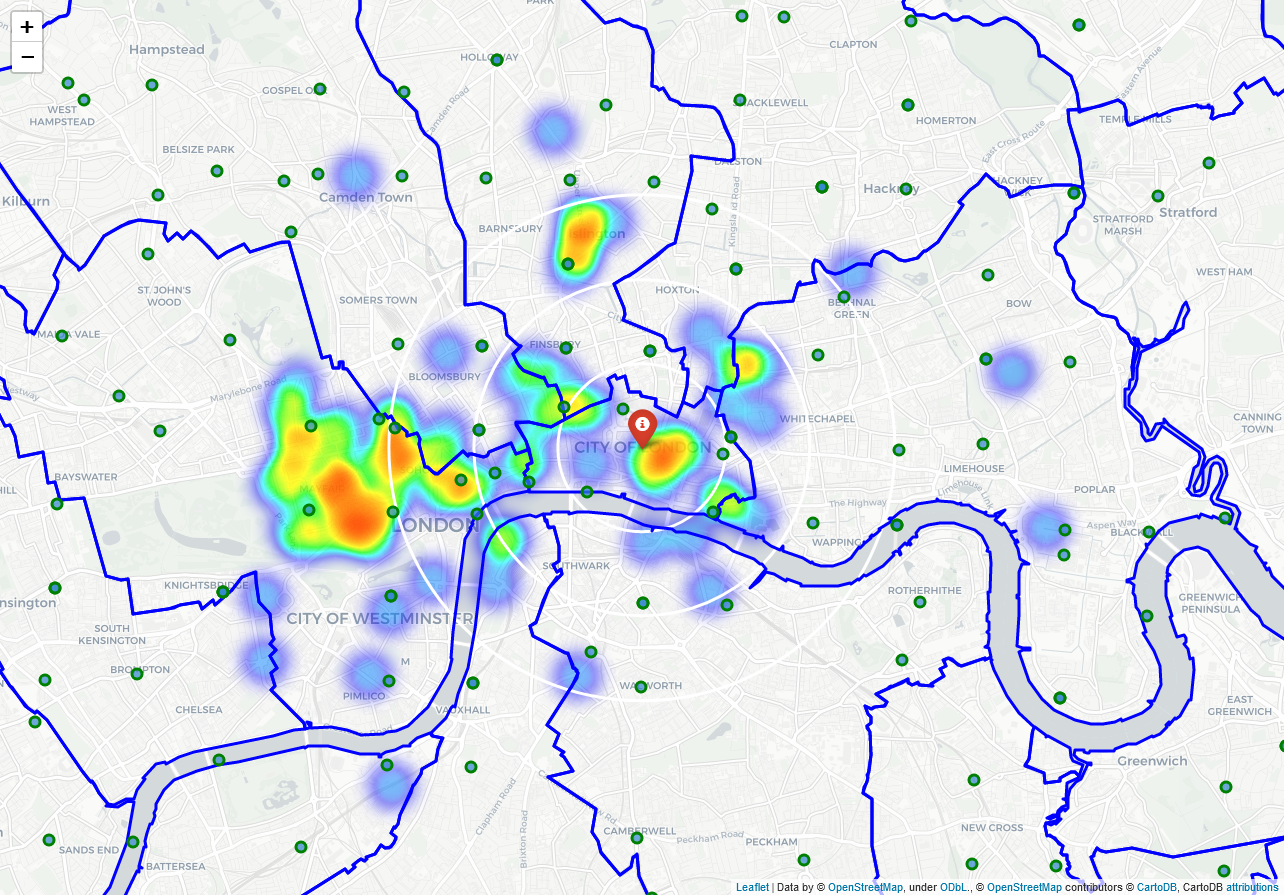
\includegraphics{11_rest_heat_fre}\end{center}

            % \begin{tcolorbox}[breakable, size=fbox, boxrule=.5pt, pad at break*=1mm, opacityfill=0]
% % \prompt{Out}{outcolor}{76}{\boxspacing}
% \begin{Verbatim}[commandchars=\\\{\}]
% <folium.folium.Map at 0x221eec8eee0>
% \end{Verbatim}
% \end{tcolorbox}
        
    % \begin{tcolorbox}[breakable, size=fbox, boxrule=1pt, pad at break*=1mm,colback=cellbackground, colframe=cellborder]
% \prompt{In}{incolor}{77}{\boxspacing}
% \begin{Verbatim}[commandchars=\\\{\}]
% \PY{n}{save\PYZus{}map}\PY{p}{(}\PY{n}{map\PYZus{}rest\PYZus{}heat\PYZus{}fre}\PY{p}{,} \PY{l+s+s1}{\PYZsq{}}\PY{l+s+s1}{11\PYZus{}rest\PYZus{}heat\PYZus{}fre}\PY{l+s+s1}{\PYZsq{}}\PY{p}{)}
% \end{Verbatim}
% \end{tcolorbox}

    % \begin{Verbatim}[commandchars=\\\{\}]
% Map saved under '11\_rest\_heat\_fre.html' and '11\_rest\_heat\_fre.png'
    % \end{Verbatim}

    That is already much better. We can clearly see that \textbf{French}
restaurants are less prevalents than the others, even in high density
areas like the western part of the city.

It confirm what we had found before. From now on, we will focus on
\textbf{French} restaurants.

We can see that most of them are located in Westminster, and that areas
around the neighborhoods of Barbican, Blackfriars, and Temple, lack
\textbf{French} restaurant. They don't lack restaurants in general
though.

Let's focus on this area. First, we will define a new, more narrow
region at the center of these three neighborhoods. Let's have a look at
its restaurant density:

    % \begin{tcolorbox}[breakable, size=fbox, boxrule=1pt, pad at break*=1mm,colback=cellbackground, colframe=cellborder]
% \prompt{In}{incolor}{78}{\boxspacing}
% \begin{Verbatim}[commandchars=\\\{\}]
% \PY{n}{search\PYZus{}area\PYZus{}center\PYZus{}lat} \PY{o}{=} \PY{n+nb}{sum}\PY{p}{(}\PY{n}{neigh\PYZus{}data}\PY{o}{.}\PY{n}{loc}\PY{p}{[}\PY{n}{neigh\PYZus{}data}\PY{p}{[}\PY{l+s+s1}{\PYZsq{}}\PY{l+s+s1}{Neighborhood}\PY{l+s+s1}{\PYZsq{}}\PY{p}{]}\PY{o}{.}\PY{n}{isin}\PY{p}{(}\PY{p}{[}\PY{l+s+s1}{\PYZsq{}}\PY{l+s+s1}{Barbican}\PY{l+s+s1}{\PYZsq{}}\PY{p}{,}\PY{l+s+s1}{\PYZsq{}}\PY{l+s+s1}{Blackfriars}\PY{l+s+s1}{\PYZsq{}}\PY{p}{,}\PY{l+s+s1}{\PYZsq{}}\PY{l+s+s1}{Temple}\PY{l+s+s1}{\PYZsq{}}\PY{p}{]}\PY{p}{)}\PY{p}{,} \PY{l+s+s1}{\PYZsq{}}\PY{l+s+s1}{Latitude}\PY{l+s+s1}{\PYZsq{}}\PY{p}{]}\PY{p}{)} \PY{o}{/} \PY{l+m+mi}{3}
% \PY{n}{search\PYZus{}area\PYZus{}center\PYZus{}long} \PY{o}{=} \PY{n+nb}{sum}\PY{p}{(}\PY{n}{neigh\PYZus{}data}\PY{o}{.}\PY{n}{loc}\PY{p}{[}\PY{n}{neigh\PYZus{}data}\PY{p}{[}\PY{l+s+s1}{\PYZsq{}}\PY{l+s+s1}{Neighborhood}\PY{l+s+s1}{\PYZsq{}}\PY{p}{]}\PY{o}{.}\PY{n}{isin}\PY{p}{(}\PY{p}{[}\PY{l+s+s1}{\PYZsq{}}\PY{l+s+s1}{Barbican}\PY{l+s+s1}{\PYZsq{}}\PY{p}{,}\PY{l+s+s1}{\PYZsq{}}\PY{l+s+s1}{Blackfriars}\PY{l+s+s1}{\PYZsq{}}\PY{p}{,}\PY{l+s+s1}{\PYZsq{}}\PY{l+s+s1}{Temple}\PY{l+s+s1}{\PYZsq{}}\PY{p}{]}\PY{p}{)}\PY{p}{,} \PY{l+s+s1}{\PYZsq{}}\PY{l+s+s1}{Longitude}\PY{l+s+s1}{\PYZsq{}}\PY{p}{]}\PY{p}{)} \PY{o}{/} \PY{l+m+mi}{3}

% \PY{n+nb}{print}\PY{p}{(}\PY{l+s+s2}{\PYZdq{}}\PY{l+s+s2}{Center: }\PY{l+s+si}{\PYZob{}\PYZcb{}}\PY{l+s+s2}{, }\PY{l+s+si}{\PYZob{}\PYZcb{}}\PY{l+s+s2}{\PYZdq{}}\PY{o}{.}\PY{n}{format}\PY{p}{(}\PY{n}{search\PYZus{}area\PYZus{}center\PYZus{}lat}\PY{p}{,} \PY{n}{search\PYZus{}area\PYZus{}center\PYZus{}long}\PY{p}{)}\PY{p}{)}
% \end{Verbatim}
% \end{tcolorbox}

    \begin{Verbatim}[commandchars=\\\{\}]
Center: 51.51408470892323, -0.10291062852174855
    \end{Verbatim}

    % \begin{tcolorbox}[breakable, size=fbox, boxrule=1pt, pad at break*=1mm,colback=cellbackground, colframe=cellborder]
% \prompt{In}{incolor}{79}{\boxspacing}
% \begin{Verbatim}[commandchars=\\\{\}]
% \PY{n}{map\PYZus{}search\PYZus{}area} \PY{o}{=} \PY{n}{folium}\PY{o}{.}\PY{n}{Map}\PY{p}{(}\PY{n}{location}\PY{o}{=}\PY{p}{[}\PY{n}{search\PYZus{}area\PYZus{}center\PYZus{}lat}\PY{p}{,} \PY{n}{search\PYZus{}area\PYZus{}center\PYZus{}long}\PY{p}{]}\PY{p}{,} \PY{n}{zoom\PYZus{}start}\PY{o}{=}\PY{l+m+mi}{15}\PY{p}{)}
% \PY{n}{HeatMap}\PY{p}{(}\PY{n}{restaurant\PYZus{}latlong}\PY{p}{)}\PY{o}{.}\PY{n}{add\PYZus{}to}\PY{p}{(}\PY{n}{map\PYZus{}search\PYZus{}area}\PY{p}{)}
% \PY{n}{folium}\PY{o}{.}\PY{n}{Marker}\PY{p}{(}\PY{p}{[}\PY{n}{city\PYZus{}latitude}\PY{p}{,} \PY{n}{city\PYZus{}longitude}\PY{p}{]}\PY{p}{,} \PY{n}{icon}\PY{o}{=}\PY{n}{folium}\PY{o}{.}\PY{n}{Icon}\PY{p}{(}\PY{n}{color}\PY{o}{=}\PY{l+s+s1}{\PYZsq{}}\PY{l+s+s1}{red}\PY{l+s+s1}{\PYZsq{}}\PY{p}{,} \PY{n}{icon}\PY{o}{=}\PY{l+s+s1}{\PYZsq{}}\PY{l+s+s1}{info\PYZhy{}sign}\PY{l+s+s1}{\PYZsq{}}\PY{p}{)}\PY{p}{,} \PY{n}{popup}\PY{o}{=}\PY{l+s+s1}{\PYZsq{}}\PY{l+s+s1}{City Center}\PY{l+s+s1}{\PYZsq{}}\PY{p}{)}\PY{o}{.}\PY{n}{add\PYZus{}to}\PY{p}{(}\PY{n}{map\PYZus{}search\PYZus{}area}\PY{p}{)}
% \PY{n}{folium}\PY{o}{.}\PY{n}{Circle}\PY{p}{(}\PY{p}{[}\PY{n}{search\PYZus{}area\PYZus{}center\PYZus{}lat}\PY{p}{,} \PY{n}{search\PYZus{}area\PYZus{}center\PYZus{}long}\PY{p}{]}\PY{p}{,} \PY{n}{radius}\PY{o}{=}\PY{l+m+mi}{1000}\PY{p}{,} \PY{n}{color}\PY{o}{=}\PY{l+s+s1}{\PYZsq{}}\PY{l+s+s1}{white}\PY{l+s+s1}{\PYZsq{}}\PY{p}{,} \PY{n}{fill}\PY{o}{=}\PY{k+kc}{True}\PY{p}{,} \PY{n}{fill\PYZus{}opacity}\PY{o}{=}\PY{l+m+mf}{0.4}\PY{p}{)}\PY{o}{.}\PY{n}{add\PYZus{}to}\PY{p}{(}\PY{n}{map\PYZus{}search\PYZus{}area}\PY{p}{)}
% \PY{n}{folium}\PY{o}{.}\PY{n}{GeoJson}\PY{p}{(}\PY{n}{london\PYZus{}boroughs\PYZus{}boundaries}\PY{p}{,} \PY{n}{style\PYZus{}function}\PY{o}{=}\PY{n}{boroughs\PYZus{}style}\PY{p}{,} \PY{n}{name}\PY{o}{=}\PY{l+s+s1}{\PYZsq{}}\PY{l+s+s1}{geojson}\PY{l+s+s1}{\PYZsq{}}\PY{p}{)}\PY{o}{.}\PY{n}{add\PYZus{}to}\PY{p}{(}\PY{n}{map\PYZus{}search\PYZus{}area}\PY{p}{)}
% \PY{n}{map\PYZus{}search\PYZus{}area}
% \end{Verbatim}
% \end{tcolorbox}

\begin{center}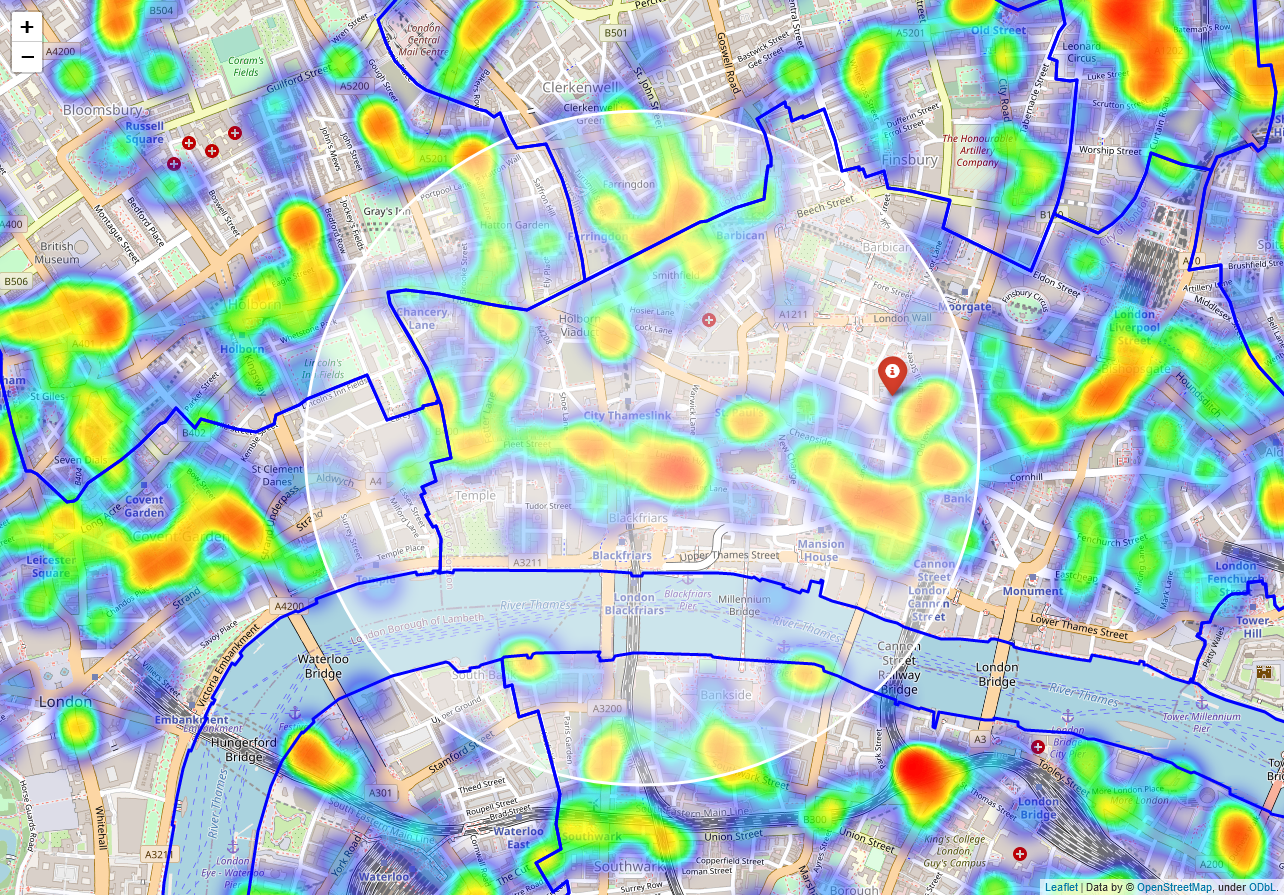
\includegraphics{12_search_area}\end{center}

            % \begin{tcolorbox}[breakable, size=fbox, boxrule=.5pt, pad at break*=1mm, opacityfill=0]
% % \prompt{Out}{outcolor}{79}{\boxspacing}
% \begin{Verbatim}[commandchars=\\\{\}]
% <folium.folium.Map at 0x221ef510550>
% \end{Verbatim}
% \end{tcolorbox}
        
    % \begin{tcolorbox}[breakable, size=fbox, boxrule=1pt, pad at break*=1mm,colback=cellbackground, colframe=cellborder]
% \prompt{In}{incolor}{80}{\boxspacing}
% \begin{Verbatim}[commandchars=\\\{\}]
% \PY{n}{save\PYZus{}map}\PY{p}{(}\PY{n}{map\PYZus{}search\PYZus{}area}\PY{p}{,} \PY{l+s+s1}{\PYZsq{}}\PY{l+s+s1}{12\PYZus{}search\PYZus{}area}\PY{l+s+s1}{\PYZsq{}}\PY{p}{)}
% \end{Verbatim}
% \end{tcolorbox}

    % \begin{Verbatim}[commandchars=\\\{\}]
% Map saved under '12\_search\_area.html' and '12\_search\_area.png'
    % \end{Verbatim}

    Perfect. It covers nicely our area of interest.

Let's also create new, more dense grid of location candidates. We will
make our candidates 100m appart, on a 1x1km hexagone:

    % \begin{tcolorbox}[breakable, size=fbox, boxrule=1pt, pad at break*=1mm,colback=cellbackground, colframe=cellborder]
% \prompt{In}{incolor}{81}{\boxspacing}
% \begin{Verbatim}[commandchars=\\\{\}]
% \PY{n}{search\PYZus{}area\PYZus{}center\PYZus{}x}\PY{p}{,} \PY{n}{search\PYZus{}area\PYZus{}center\PYZus{}y} \PY{o}{=} \PY{n}{lonlat\PYZus{}to\PYZus{}xy}\PY{p}{(}\PY{n}{search\PYZus{}area\PYZus{}center\PYZus{}long}\PY{p}{,} \PY{n}{search\PYZus{}area\PYZus{}center\PYZus{}lat}\PY{p}{)} \PY{c+c1}{\PYZsh{} City center in Cartesian coordinates}

% \PY{n}{k} \PY{o}{=} \PY{n}{math}\PY{o}{.}\PY{n}{sqrt}\PY{p}{(}\PY{l+m+mi}{3}\PY{p}{)} \PY{o}{/} \PY{l+m+mi}{2} \PY{c+c1}{\PYZsh{} Vertical offset for hexagonal grid cells}
% \PY{n}{x\PYZus{}step} \PY{o}{=} \PY{l+m+mi}{100}
% \PY{n}{y\PYZus{}step} \PY{o}{=} \PY{l+m+mi}{100} \PY{o}{*} \PY{n}{k}
% \PY{n}{sa\PYZus{}x\PYZus{}min} \PY{o}{=} \PY{n}{search\PYZus{}area\PYZus{}center\PYZus{}x} \PY{o}{\PYZhy{}} \PY{l+m+mi}{1000}
% \PY{n}{sa\PYZus{}y\PYZus{}min} \PY{o}{=} \PY{n}{search\PYZus{}area\PYZus{}center\PYZus{}y} \PY{o}{\PYZhy{}} \PY{l+m+mi}{1000}

% \PY{n}{sa\PYZus{}lat\PYZus{}all} \PY{o}{=} \PY{p}{[}\PY{p}{]}
% \PY{n}{sa\PYZus{}long\PYZus{}all} \PY{o}{=} \PY{p}{[}\PY{p}{]}
% \PY{n}{sa\PYZus{}xs\PYZus{}all} \PY{o}{=} \PY{p}{[}\PY{p}{]}
% \PY{n}{sa\PYZus{}ys\PYZus{}all} \PY{o}{=} \PY{p}{[}\PY{p}{]}
% \PY{k}{for} \PY{n}{i} \PY{o+ow}{in} \PY{n+nb}{range}\PY{p}{(}\PY{l+m+mi}{0}\PY{p}{,} \PY{n+nb}{int}\PY{p}{(}\PY{l+m+mi}{51}\PY{o}{/}\PY{n}{k}\PY{p}{)}\PY{p}{)}\PY{p}{:}
    % \PY{n}{y} \PY{o}{=} \PY{n}{sa\PYZus{}y\PYZus{}min} \PY{o}{+} \PY{n}{i} \PY{o}{*} \PY{n}{y\PYZus{}step}
    % \PY{n}{x\PYZus{}offset} \PY{o}{=} \PY{l+m+mi}{50} \PY{k}{if} \PY{n}{i}\PY{o}{\PYZpc{}}\PY{k}{2}==0 else 0
    % \PY{k}{for} \PY{n}{j} \PY{o+ow}{in} \PY{n+nb}{range}\PY{p}{(}\PY{l+m+mi}{0}\PY{p}{,} \PY{l+m+mi}{51}\PY{p}{)}\PY{p}{:}
        % \PY{n}{x} \PY{o}{=} \PY{n}{sa\PYZus{}x\PYZus{}min} \PY{o}{+} \PY{n}{j} \PY{o}{*} \PY{n}{x\PYZus{}step} \PY{o}{+} \PY{n}{x\PYZus{}offset}
        % \PY{n}{d} \PY{o}{=} \PY{n}{calc\PYZus{}xy\PYZus{}distance}\PY{p}{(}\PY{n}{search\PYZus{}area\PYZus{}center\PYZus{}x}\PY{p}{,} \PY{n}{search\PYZus{}area\PYZus{}center\PYZus{}y}\PY{p}{,} \PY{n}{x}\PY{p}{,} \PY{n}{y}\PY{p}{)}
        % \PY{k}{if} \PY{p}{(}\PY{n}{d} \PY{o}{\PYZlt{}}\PY{o}{=} \PY{l+m+mi}{1001}\PY{p}{)}\PY{p}{:}
            % \PY{n}{lon}\PY{p}{,} \PY{n}{lat} \PY{o}{=} \PY{n}{xy\PYZus{}to\PYZus{}lonlat}\PY{p}{(}\PY{n}{x}\PY{p}{,} \PY{n}{y}\PY{p}{)}
            % \PY{n}{sa\PYZus{}lat\PYZus{}all}\PY{o}{.}\PY{n}{append}\PY{p}{(}\PY{n}{lat}\PY{p}{)}
            % \PY{n}{sa\PYZus{}long\PYZus{}all}\PY{o}{.}\PY{n}{append}\PY{p}{(}\PY{n}{lon}\PY{p}{)}
            % \PY{n}{sa\PYZus{}xs\PYZus{}all}\PY{o}{.}\PY{n}{append}\PY{p}{(}\PY{n}{x}\PY{p}{)}
            % \PY{n}{sa\PYZus{}ys\PYZus{}all}\PY{o}{.}\PY{n}{append}\PY{p}{(}\PY{n}{y}\PY{p}{)}

% \PY{n+nb}{print}\PY{p}{(}\PY{n+nb}{len}\PY{p}{(}\PY{n}{sa\PYZus{}lat\PYZus{}all}\PY{p}{)}\PY{p}{,} \PY{l+s+s1}{\PYZsq{}}\PY{l+s+s1}{candidate neighborhood centers generated.}\PY{l+s+s1}{\PYZsq{}}\PY{p}{)}
% \end{Verbatim}
% \end{tcolorbox}

% \resizebox{\textwidth}{!}{%
    \begin{tabular}{llll}
    362 candidate neighborhood centers generated.
    \\\hline
    Latitude & Longitude & X & Y
    \\ \hline
    51.506024 & -0.109187 & 700613.6619 & 5.710062e+06
    \\
    51.505989 & -0.107748 & 700713.6619 & 5.710062e+06
    \\
    51.505953 & -0.106309 & 700813.6619 & 5.710062e+06
    \\
    51.505918 & -0.104870 & 700913.6619 & 5.710062e+06
    \\
    51.505882 & -0.103431 & 701013.6619 & 5.710062e+06
    \end{tabular}
% }

    % \begin{Verbatim}[commandchars=\\\{\}]
% 362 candidate neighborhood centers generated.
    % \end{Verbatim}

    % \begin{tcolorbox}[breakable, size=fbox, boxrule=1pt, pad at break*=1mm,colback=cellbackground, colframe=cellborder]
% \prompt{In}{incolor}{82}{\boxspacing}
% \begin{Verbatim}[commandchars=\\\{\}]
% \PY{n}{sa\PYZus{}all} \PY{o}{=} \PY{n}{pd}\PY{o}{.}\PY{n}{DataFrame}\PY{p}{(}\PY{n+nb}{list}\PY{p}{(}\PY{n+nb}{zip}\PY{p}{(}\PY{n}{sa\PYZus{}lat\PYZus{}all}\PY{p}{,} \PY{n}{sa\PYZus{}long\PYZus{}all}\PY{p}{,} \PY{n}{sa\PYZus{}xs\PYZus{}all}\PY{p}{,} \PY{n}{sa\PYZus{}ys\PYZus{}all}\PY{p}{)}\PY{p}{)}\PY{p}{,}
                        % \PY{n}{columns}\PY{o}{=}\PY{p}{[}\PY{l+s+s1}{\PYZsq{}}\PY{l+s+s1}{Latitude}\PY{l+s+s1}{\PYZsq{}}\PY{p}{,}\PY{l+s+s1}{\PYZsq{}}\PY{l+s+s1}{Longitude}\PY{l+s+s1}{\PYZsq{}}\PY{p}{,}\PY{l+s+s1}{\PYZsq{}}\PY{l+s+s1}{X}\PY{l+s+s1}{\PYZsq{}}\PY{p}{,}\PY{l+s+s1}{\PYZsq{}}\PY{l+s+s1}{Y}\PY{l+s+s1}{\PYZsq{}}\PY{p}{]}\PY{p}{)}
% \PY{n}{sa\PYZus{}all}\PY{o}{.}\PY{n}{head}\PY{p}{(}\PY{p}{)}
% \end{Verbatim}
% \end{tcolorbox}

            % \begin{tcolorbox}[breakable, size=fbox, boxrule=.5pt, pad at break*=1mm, opacityfill=0]
% % \prompt{Out}{outcolor}{82}{\boxspacing}
% \begin{Verbatim}[commandchars=\\\{\}]
    % Latitude  Longitude            X             Y
% 0  51.506024  -0.109187  700613.6619  5.710062e+06
% 1  51.505989  -0.107748  700713.6619  5.710062e+06
% 2  51.505953  -0.106309  700813.6619  5.710062e+06
% 3  51.505918  -0.104870  700913.6619  5.710062e+06
% 4  51.505882  -0.103431  701013.6619  5.710062e+06
% \end{Verbatim}
% \end{tcolorbox}
        
    Let's see that grid on a map:

    % \begin{tcolorbox}[breakable, size=fbox, boxrule=1pt, pad at break*=1mm,colback=cellbackground, colframe=cellborder]
% \prompt{In}{incolor}{83}{\boxspacing}
% \begin{Verbatim}[commandchars=\\\{\}]
% \PY{n}{map\PYZus{}hexa\PYZus{}sa\PYZus{}all} \PY{o}{=} \PY{n}{folium}\PY{o}{.}\PY{n}{Map}\PY{p}{(}\PY{n}{location}\PY{o}{=}\PY{p}{[}\PY{n}{search\PYZus{}area\PYZus{}center\PYZus{}lat}\PY{p}{,} \PY{n}{search\PYZus{}area\PYZus{}center\PYZus{}long}\PY{p}{]}\PY{p}{,} \PY{n}{zoom\PYZus{}start}\PY{o}{=}\PY{l+m+mi}{15}\PY{p}{)}
% \PY{n}{folium}\PY{o}{.}\PY{n}{Marker}\PY{p}{(}\PY{p}{[}\PY{n}{city\PYZus{}latitude}\PY{p}{,} \PY{n}{city\PYZus{}longitude}\PY{p}{]}\PY{p}{,} \PY{n}{icon}\PY{o}{=}\PY{n}{folium}\PY{o}{.}\PY{n}{Icon}\PY{p}{(}\PY{n}{color}\PY{o}{=}\PY{l+s+s1}{\PYZsq{}}\PY{l+s+s1}{red}\PY{l+s+s1}{\PYZsq{}}\PY{p}{,} \PY{n}{icon}\PY{o}{=}\PY{l+s+s1}{\PYZsq{}}\PY{l+s+s1}{info\PYZhy{}sign}\PY{l+s+s1}{\PYZsq{}}\PY{p}{)}\PY{p}{,} \PY{n}{popup}\PY{o}{=}\PY{l+s+s1}{\PYZsq{}}\PY{l+s+s1}{City Center}\PY{l+s+s1}{\PYZsq{}}\PY{p}{)}\PY{o}{.}\PY{n}{add\PYZus{}to}\PY{p}{(}\PY{n}{map\PYZus{}hexa\PYZus{}sa\PYZus{}all}\PY{p}{)}
% \PY{k}{for} \PY{n}{lat}\PY{p}{,} \PY{n}{lon} \PY{o+ow}{in} \PY{n+nb}{zip}\PY{p}{(}\PY{n}{sa\PYZus{}lat\PYZus{}all}\PY{p}{,} \PY{n}{sa\PYZus{}long\PYZus{}all}\PY{p}{)}\PY{p}{:}
    % \PY{c+c1}{\PYZsh{}folium.CircleMarker([lat, lon], radius=2, color=\PYZsq{}blue\PYZsq{}, fill=True, fill\PYZus{}color=\PYZsq{}blue\PYZsq{}, fill\PYZus{}opacity=1).add\PYZus{}to(map\PYZus{}berlin) }
    % \PY{n}{folium}\PY{o}{.}\PY{n}{Circle}\PY{p}{(}\PY{p}{[}\PY{n}{lat}\PY{p}{,} \PY{n}{lon}\PY{p}{]}\PY{p}{,} \PY{n}{radius}\PY{o}{=}\PY{l+m+mi}{50}\PY{p}{,} \PY{n}{color}\PY{o}{=}\PY{l+s+s1}{\PYZsq{}}\PY{l+s+s1}{blue}\PY{l+s+s1}{\PYZsq{}}\PY{p}{,} \PY{n}{fill}\PY{o}{=}\PY{k+kc}{False}\PY{p}{)}\PY{o}{.}\PY{n}{add\PYZus{}to}\PY{p}{(}\PY{n}{map\PYZus{}hexa\PYZus{}sa\PYZus{}all}\PY{p}{)}
    % \PY{c+c1}{\PYZsh{}folium.Marker([lat, lon]).add\PYZus{}to(map\PYZus{}berlin)}
% \PY{n}{map\PYZus{}hexa\PYZus{}sa\PYZus{}all}
% \end{Verbatim}
% \end{tcolorbox}

\begin{center}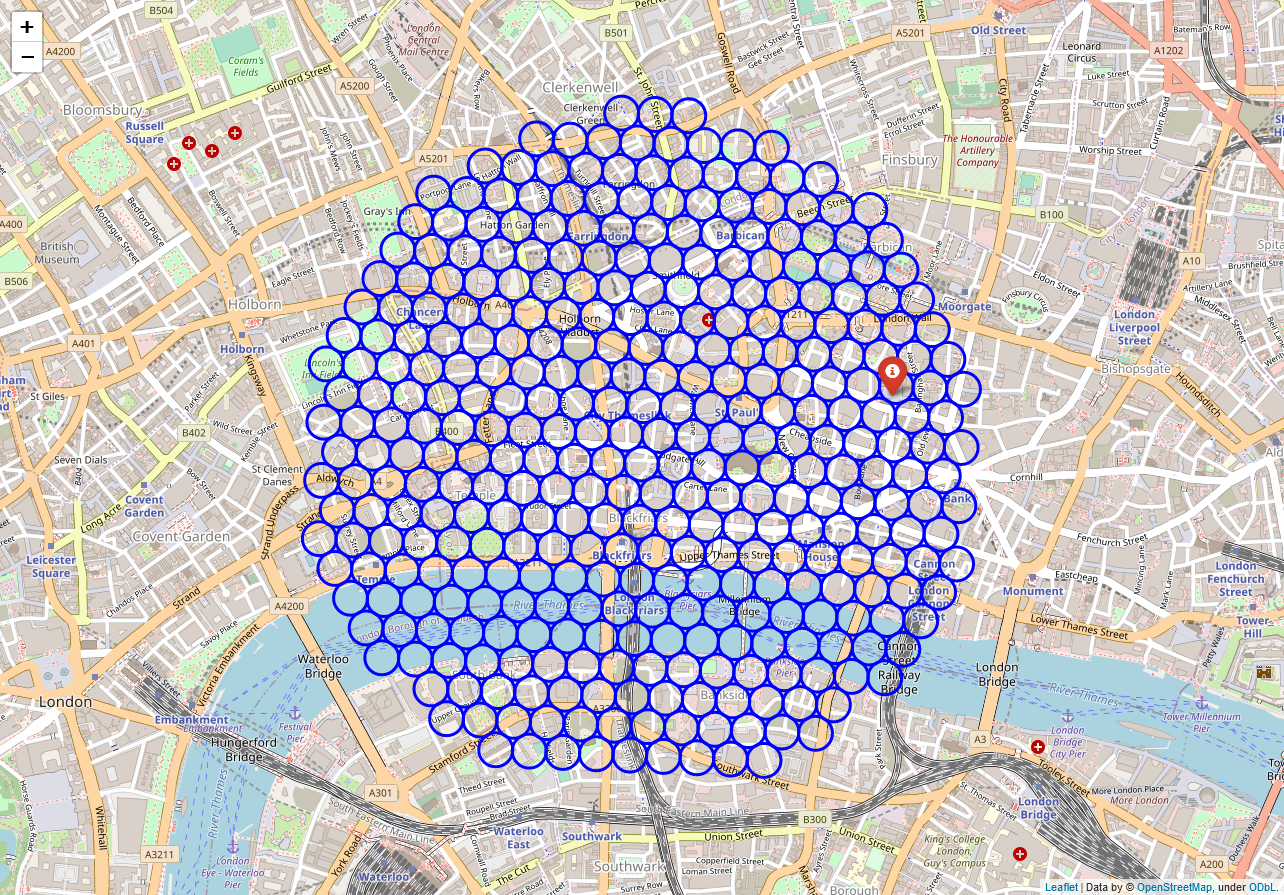
\includegraphics{13_hexa_sa_all}\end{center}

            % \begin{tcolorbox}[breakable, size=fbox, boxrule=.5pt, pad at break*=1mm, opacityfill=0]
% % \prompt{Out}{outcolor}{83}{\boxspacing}
% \begin{Verbatim}[commandchars=\\\{\}]
% <folium.folium.Map at 0x221ef58a0a0>
% \end{Verbatim}
% \end{tcolorbox}
        
    % \begin{tcolorbox}[breakable, size=fbox, boxrule=1pt, pad at break*=1mm,colback=cellbackground, colframe=cellborder]
% \prompt{In}{incolor}{84}{\boxspacing}
% \begin{Verbatim}[commandchars=\\\{\}]
% \PY{n}{save\PYZus{}map}\PY{p}{(}\PY{n}{map\PYZus{}hexa\PYZus{}sa\PYZus{}all}\PY{p}{,} \PY{l+s+s1}{\PYZsq{}}\PY{l+s+s1}{13\PYZus{}hexa\PYZus{}sa\PYZus{}all}\PY{l+s+s1}{\PYZsq{}}\PY{p}{)}
% \end{Verbatim}
% \end{tcolorbox}

    % \begin{Verbatim}[commandchars=\\\{\}]
% Map saved under '13\_hexa\_sa\_all.html' and '13\_hexa\_sa\_all.png'
    % \end{Verbatim}

    Once again, the River Thames is a problem.

Let's mimict what we did and remove bad areas:

    % \begin{tcolorbox}[breakable, size=fbox, boxrule=1pt, pad at break*=1mm,colback=cellbackground, colframe=cellborder]
% \prompt{In}{incolor}{85}{\boxspacing}
% \begin{Verbatim}[commandchars=\\\{\}]
% \PY{n}{sa\PYZus{}lat\PYZus{}bad} \PY{o}{=} \PY{p}{[}\PY{p}{]}
% \PY{n}{sa\PYZus{}long\PYZus{}bad} \PY{o}{=} \PY{p}{[}\PY{p}{]}
% \PY{n}{sa\PYZus{}xs\PYZus{}bad} \PY{o}{=} \PY{p}{[}\PY{p}{]}
% \PY{n}{sa\PYZus{}ys\PYZus{}bad} \PY{o}{=} \PY{p}{[}\PY{p}{]}

% \PY{k}{for} \PY{n}{lat}\PY{p}{,} \PY{n}{long}\PY{p}{,} \PY{n}{x}\PY{p}{,} \PY{n}{y} \PY{o+ow}{in} \PY{n+nb}{zip}\PY{p}{(}\PY{n}{sa\PYZus{}lat\PYZus{}all}\PY{p}{,} \PY{n}{sa\PYZus{}long\PYZus{}all}\PY{p}{,} \PY{n}{sa\PYZus{}xs\PYZus{}all}\PY{p}{,} \PY{n}{sa\PYZus{}ys\PYZus{}all}\PY{p}{)}\PY{p}{:}
    % \PY{n}{point} \PY{o}{=} \PY{n}{Point}\PY{p}{(}\PY{n}{long}\PY{p}{,} \PY{n}{lat}\PY{p}{)}
    % \PY{c+c1}{\PYZsh{} River Thames}
    % \PY{k}{for} \PY{n}{feature} \PY{o+ow}{in} \PY{n}{thames}\PY{p}{[}\PY{l+s+s1}{\PYZsq{}}\PY{l+s+s1}{features}\PY{l+s+s1}{\PYZsq{}}\PY{p}{]}\PY{p}{:}
        % \PY{n}{polygon} \PY{o}{=} \PY{n}{shape}\PY{p}{(}\PY{n}{feature}\PY{p}{[}\PY{l+s+s1}{\PYZsq{}}\PY{l+s+s1}{geometry}\PY{l+s+s1}{\PYZsq{}}\PY{p}{]}\PY{p}{)}
        % \PY{k}{if} \PY{n}{polygon}\PY{o}{.}\PY{n}{contains}\PY{p}{(}\PY{n}{point}\PY{p}{)}\PY{p}{:}
            % \PY{n}{sa\PYZus{}lat\PYZus{}bad}\PY{o}{.}\PY{n}{append}\PY{p}{(}\PY{n}{lat}\PY{p}{)}
            % \PY{n}{sa\PYZus{}long\PYZus{}bad}\PY{o}{.}\PY{n}{append}\PY{p}{(}\PY{n}{long}\PY{p}{)}
            % \PY{n}{sa\PYZus{}xs\PYZus{}bad}\PY{o}{.}\PY{n}{append}\PY{p}{(}\PY{n}{x}\PY{p}{)}
            % \PY{n}{sa\PYZus{}ys\PYZus{}bad}\PY{o}{.}\PY{n}{append}\PY{p}{(}\PY{n}{y}\PY{p}{)}
            % \PY{k}{break}
% \PY{n+nb}{print}\PY{p}{(}\PY{l+s+s1}{\PYZsq{}}\PY{l+s+si}{\PYZob{}\PYZcb{}}\PY{l+s+s1}{ coordinates to be removed out of }\PY{l+s+si}{\PYZob{}\PYZcb{}}\PY{l+s+s1}{\PYZsq{}}\PY{o}{.}\PY{n}{format}\PY{p}{(}\PY{n+nb}{len}\PY{p}{(}\PY{n}{sa\PYZus{}lat\PYZus{}bad}\PY{p}{)}\PY{p}{,} \PY{n+nb}{len}\PY{p}{(}\PY{n}{sa\PYZus{}lat\PYZus{}all}\PY{p}{)}\PY{p}{)}\PY{p}{)}
% \end{Verbatim}
% \end{tcolorbox}

% \resizebox{\textwidth}{!}{%
    \begin{tabular}{llll}
    50 coordinates to be removed out of 362
    \\\hline
    Latitude & Longitude & X & Y
    \\ \hline
    51.508482 & -0.114076 & 700263.6619 & 5.710321e+06
    \\
    51.508446 & -0.112637 & 700363.6619 & 5.710321e+06
    \\
    51.508375 & -0.109759 & 700563.6619 & 5.710321e+06
    \\
    51.507984 & -0.093929 & 701663.6619 & 5.710321e+06
    \\
    51.507948 & -0.092490 & 701763.6619 & 5.710321e+06
    \end{tabular}
% }

    % \begin{Verbatim}[commandchars=\\\{\}]
% 50 coordinates to be removed out of 362
    % \end{Verbatim}

    % \begin{tcolorbox}[breakable, size=fbox, boxrule=1pt, pad at break*=1mm,colback=cellbackground, colframe=cellborder]
% \prompt{In}{incolor}{86}{\boxspacing}
% \begin{Verbatim}[commandchars=\\\{\}]
% \PY{n}{sa\PYZus{}bad} \PY{o}{=} \PY{n}{pd}\PY{o}{.}\PY{n}{DataFrame}\PY{p}{(}\PY{n+nb}{list}\PY{p}{(}\PY{n+nb}{zip}\PY{p}{(}\PY{n}{sa\PYZus{}lat\PYZus{}bad}\PY{p}{,} \PY{n}{sa\PYZus{}long\PYZus{}bad}\PY{p}{,} \PY{n}{sa\PYZus{}xs\PYZus{}bad}\PY{p}{,} \PY{n}{sa\PYZus{}ys\PYZus{}bad}\PY{p}{)}\PY{p}{)}\PY{p}{,}
                        % \PY{n}{columns}\PY{o}{=}\PY{p}{[}\PY{l+s+s1}{\PYZsq{}}\PY{l+s+s1}{Latitude}\PY{l+s+s1}{\PYZsq{}}\PY{p}{,}\PY{l+s+s1}{\PYZsq{}}\PY{l+s+s1}{Longitude}\PY{l+s+s1}{\PYZsq{}}\PY{p}{,}\PY{l+s+s1}{\PYZsq{}}\PY{l+s+s1}{X}\PY{l+s+s1}{\PYZsq{}}\PY{p}{,}\PY{l+s+s1}{\PYZsq{}}\PY{l+s+s1}{Y}\PY{l+s+s1}{\PYZsq{}}\PY{p}{]}\PY{p}{)}
% \PY{n}{sa\PYZus{}bad}\PY{o}{.}\PY{n}{head}\PY{p}{(}\PY{p}{)}
% \end{Verbatim}
% \end{tcolorbox}

            % \begin{tcolorbox}[breakable, size=fbox, boxrule=.5pt, pad at break*=1mm, opacityfill=0]
% % \prompt{Out}{outcolor}{86}{\boxspacing}
% \begin{Verbatim}[commandchars=\\\{\}]
    % Latitude  Longitude            X             Y
% 0  51.508482  -0.114076  700263.6619  5.710321e+06
% 1  51.508446  -0.112637  700363.6619  5.710321e+06
% 2  51.508375  -0.109759  700563.6619  5.710321e+06
% 3  51.507984  -0.093929  701663.6619  5.710321e+06
% 4  51.507948  -0.092490  701763.6619  5.710321e+06
% \end{Verbatim}
% \end{tcolorbox}
        
    % \begin{tcolorbox}[breakable, size=fbox, boxrule=1pt, pad at break*=1mm,colback=cellbackground, colframe=cellborder]
% \prompt{In}{incolor}{87}{\boxspacing}
% \begin{Verbatim}[commandchars=\\\{\}]
% \PY{n}{map\PYZus{}hexa\PYZus{}sa\PYZus{}bad} \PY{o}{=} \PY{n}{folium}\PY{o}{.}\PY{n}{Map}\PY{p}{(}\PY{n}{location}\PY{o}{=}\PY{p}{[}\PY{n}{search\PYZus{}area\PYZus{}center\PYZus{}lat}\PY{p}{,} \PY{n}{search\PYZus{}area\PYZus{}center\PYZus{}long}\PY{p}{]}\PY{p}{,} \PY{n}{zoom\PYZus{}start}\PY{o}{=}\PY{l+m+mi}{15}\PY{p}{)}
% \PY{n}{folium}\PY{o}{.}\PY{n}{Marker}\PY{p}{(}\PY{p}{[}\PY{n}{city\PYZus{}latitude}\PY{p}{,} \PY{n}{city\PYZus{}longitude}\PY{p}{]}\PY{p}{,} \PY{n}{icon}\PY{o}{=}\PY{n}{folium}\PY{o}{.}\PY{n}{Icon}\PY{p}{(}\PY{n}{color}\PY{o}{=}\PY{l+s+s1}{\PYZsq{}}\PY{l+s+s1}{red}\PY{l+s+s1}{\PYZsq{}}\PY{p}{,} \PY{n}{icon}\PY{o}{=}\PY{l+s+s1}{\PYZsq{}}\PY{l+s+s1}{info\PYZhy{}sign}\PY{l+s+s1}{\PYZsq{}}\PY{p}{)}\PY{p}{,} \PY{n}{popup}\PY{o}{=}\PY{l+s+s1}{\PYZsq{}}\PY{l+s+s1}{City Center}\PY{l+s+s1}{\PYZsq{}}\PY{p}{)}\PY{o}{.}\PY{n}{add\PYZus{}to}\PY{p}{(}\PY{n}{map\PYZus{}hexa\PYZus{}sa\PYZus{}bad}\PY{p}{)}
% \PY{k}{for} \PY{n}{lat}\PY{p}{,} \PY{n}{lon} \PY{o+ow}{in} \PY{n+nb}{zip}\PY{p}{(}\PY{n}{sa\PYZus{}lat\PYZus{}all}\PY{p}{,} \PY{n}{sa\PYZus{}long\PYZus{}all}\PY{p}{)}\PY{p}{:}
    % \PY{c+c1}{\PYZsh{}folium.CircleMarker([lat, lon], radius=2, color=\PYZsq{}blue\PYZsq{}, fill=True, fill\PYZus{}color=\PYZsq{}blue\PYZsq{}, fill\PYZus{}opacity=1).add\PYZus{}to(map\PYZus{}berlin) }
    % \PY{n}{folium}\PY{o}{.}\PY{n}{Circle}\PY{p}{(}\PY{p}{[}\PY{n}{lat}\PY{p}{,} \PY{n}{lon}\PY{p}{]}\PY{p}{,} \PY{n}{radius}\PY{o}{=}\PY{l+m+mi}{50}\PY{p}{,} \PY{n}{color}\PY{o}{=}\PY{l+s+s1}{\PYZsq{}}\PY{l+s+s1}{blue}\PY{l+s+s1}{\PYZsq{}}\PY{p}{,} \PY{n}{fill}\PY{o}{=}\PY{k+kc}{False}\PY{p}{)}\PY{o}{.}\PY{n}{add\PYZus{}to}\PY{p}{(}\PY{n}{map\PYZus{}hexa\PYZus{}sa\PYZus{}bad}\PY{p}{)}
    % \PY{c+c1}{\PYZsh{}folium.Marker([lat, lon]).add\PYZus{}to(map\PYZus{}berlin)}
% \PY{k}{for} \PY{n}{lat}\PY{p}{,} \PY{n}{lon} \PY{o+ow}{in} \PY{n+nb}{zip}\PY{p}{(}\PY{n}{sa\PYZus{}lat\PYZus{}bad}\PY{p}{,} \PY{n}{sa\PYZus{}long\PYZus{}bad}\PY{p}{)}\PY{p}{:}
    % \PY{c+c1}{\PYZsh{}folium.CircleMarker([lat, lon], radius=2, color=\PYZsq{}blue\PYZsq{}, fill=True, fill\PYZus{}color=\PYZsq{}blue\PYZsq{}, fill\PYZus{}opacity=1).add\PYZus{}to(map\PYZus{}berlin) }
    % \PY{n}{folium}\PY{o}{.}\PY{n}{Circle}\PY{p}{(}\PY{p}{[}\PY{n}{lat}\PY{p}{,} \PY{n}{lon}\PY{p}{]}\PY{p}{,} \PY{n}{radius}\PY{o}{=}\PY{l+m+mi}{50}\PY{p}{,} \PY{n}{color}\PY{o}{=}\PY{l+s+s1}{\PYZsq{}}\PY{l+s+s1}{red}\PY{l+s+s1}{\PYZsq{}}\PY{p}{,} \PY{n}{fill}\PY{o}{=}\PY{k+kc}{False}\PY{p}{)}\PY{o}{.}\PY{n}{add\PYZus{}to}\PY{p}{(}\PY{n}{map\PYZus{}hexa\PYZus{}sa\PYZus{}bad}\PY{p}{)}
    % \PY{c+c1}{\PYZsh{}folium.Marker([lat, lon]).add\PYZus{}to(map\PYZus{}berlin)}
% \PY{n}{map\PYZus{}hexa\PYZus{}sa\PYZus{}bad}
% \end{Verbatim}
% \end{tcolorbox}

\begin{center}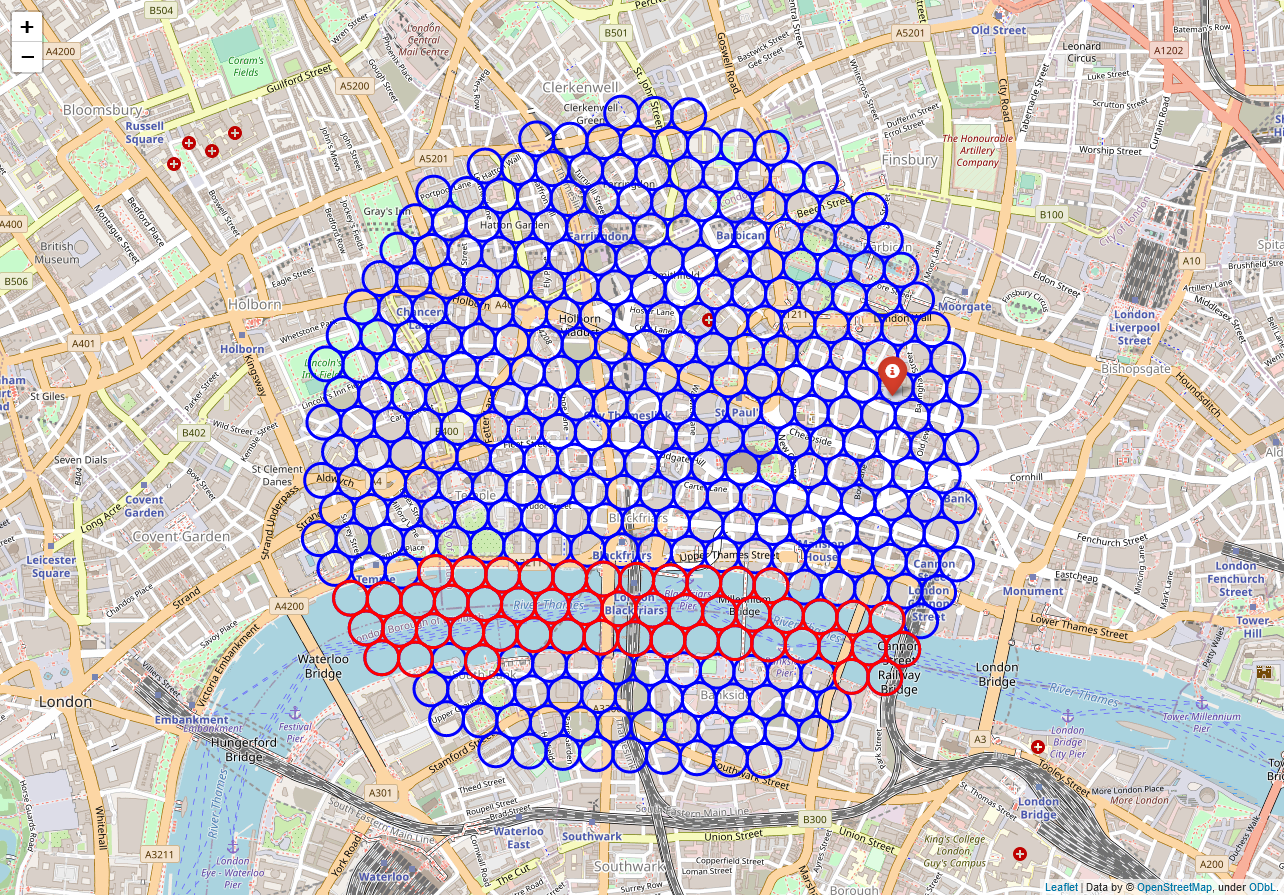
\includegraphics{14_hexa_sa_bad}\end{center}

            % \begin{tcolorbox}[breakable, size=fbox, boxrule=.5pt, pad at break*=1mm, opacityfill=0]
% % \prompt{Out}{outcolor}{87}{\boxspacing}
% \begin{Verbatim}[commandchars=\\\{\}]
% <folium.folium.Map at 0x221ef73ee80>
% \end{Verbatim}
% \end{tcolorbox}
        
    % \begin{tcolorbox}[breakable, size=fbox, boxrule=1pt, pad at break*=1mm,colback=cellbackground, colframe=cellborder]
% \prompt{In}{incolor}{88}{\boxspacing}
% \begin{Verbatim}[commandchars=\\\{\}]
% \PY{n}{save\PYZus{}map}\PY{p}{(}\PY{n}{map\PYZus{}hexa\PYZus{}sa\PYZus{}bad}\PY{p}{,} \PY{l+s+s1}{\PYZsq{}}\PY{l+s+s1}{14\PYZus{}hexa\PYZus{}sa\PYZus{}bad}\PY{l+s+s1}{\PYZsq{}}\PY{p}{)}
% \end{Verbatim}
% \end{tcolorbox}

    % \begin{Verbatim}[commandchars=\\\{\}]
% Map saved under '14\_hexa\_sa\_bad.html' and '14\_hexa\_sa\_bad.png'
    % \end{Verbatim}

    Perfect, we can now save it all into a dataframe

    % \begin{tcolorbox}[breakable, size=fbox, boxrule=1pt, pad at break*=1mm,colback=cellbackground, colframe=cellborder]
% \prompt{In}{incolor}{89}{\boxspacing}
% \begin{Verbatim}[commandchars=\\\{\}]
% \PY{n}{search\PYZus{}area} \PY{o}{=} \PY{n}{pd}\PY{o}{.}\PY{n}{merge}\PY{p}{(}\PY{n}{sa\PYZus{}all}\PY{p}{,}\PY{n}{sa\PYZus{}bad}\PY{p}{,} \PY{n}{indicator}\PY{o}{=}\PY{k+kc}{True}\PY{p}{,} \PY{n}{how}\PY{o}{=}\PY{l+s+s1}{\PYZsq{}}\PY{l+s+s1}{outer}\PY{l+s+s1}{\PYZsq{}}\PY{p}{)}\PY{o}{.}\PY{n}{query}\PY{p}{(}\PY{l+s+s1}{\PYZsq{}}\PY{l+s+s1}{\PYZus{}merge==}\PY{l+s+s1}{\PYZdq{}}\PY{l+s+s1}{left\PYZus{}only}\PY{l+s+s1}{\PYZdq{}}\PY{l+s+s1}{\PYZsq{}}\PY{p}{)}\PY{o}{.}\PY{n}{drop}\PY{p}{(}\PY{l+s+s1}{\PYZsq{}}\PY{l+s+s1}{\PYZus{}merge}\PY{l+s+s1}{\PYZsq{}}\PY{p}{,} \PY{n}{axis}\PY{o}{=}\PY{l+m+mi}{1}\PY{p}{)}\PY{o}{.}\PY{n}{reset\PYZus{}index}\PY{p}{(}\PY{n}{drop}\PY{o}{=}\PY{k+kc}{True}\PY{p}{)}
% \PY{n+nb}{print}\PY{p}{(}\PY{l+s+s2}{\PYZdq{}}\PY{l+s+s2}{Dataframe shape: }\PY{l+s+si}{\PYZob{}\PYZcb{}}\PY{l+s+s2}{\PYZdq{}}\PY{o}{.}\PY{n}{format}\PY{p}{(}\PY{n}{search\PYZus{}area}\PY{o}{.}\PY{n}{shape}\PY{p}{)}\PY{p}{)}
% \PY{n}{search\PYZus{}area}\PY{o}{.}\PY{n}{head}\PY{p}{(}\PY{p}{)}
% \end{Verbatim}
% \end{tcolorbox}

% \resizebox{\textwidth}{!}{%
    \begin{tabular}{llll}
    Dataframe shape: (312, 4)
    \\\hline
    Latitude & Longitude & X & Y
    \\ \hline
    51.506024 & -0.109187 & 700613.6619 & 5.710062e+06
    \\
    51.505989 & -0.107748 & 700713.6619 & 5.710062e+06
    \\
    51.505953 & -0.106309 & 700813.6619 & 5.710062e+06
    \\
    51.505918 & -0.104870 & 700913.6619 & 5.710062e+06
    \\
    51.505882 & -0.103431 & 701013.6619 & 5.710062e+06
    \end{tabular}
% }

    % \begin{Verbatim}[commandchars=\\\{\}]
% Dataframe shape: (312, 4)
    % \end{Verbatim}

            % \begin{tcolorbox}[breakable, size=fbox, boxrule=.5pt, pad at break*=1mm, opacityfill=0]
% % \prompt{Out}{outcolor}{89}{\boxspacing}
% \begin{Verbatim}[commandchars=\\\{\}]
    % Latitude  Longitude            X             Y
% 0  51.506024  -0.109187  700613.6619  5.710062e+06
% 1  51.505989  -0.107748  700713.6619  5.710062e+06
% 2  51.505953  -0.106309  700813.6619  5.710062e+06
% 3  51.505918  -0.104870  700913.6619  5.710062e+06
% 4  51.505882  -0.103431  701013.6619  5.710062e+06
% \end{Verbatim}
% \end{tcolorbox}
        
    Once again, let's add the corresponding addresses, using the same
procedure as before:

    % \begin{tcolorbox}[breakable, size=fbox, boxrule=1pt, pad at break*=1mm,colback=cellbackground, colframe=cellborder]
% \prompt{In}{incolor}{90}{\boxspacing}
% \begin{Verbatim}[commandchars=\\\{\}]
% \PY{n}{search\PYZus{}area}\PY{p}{[}\PY{l+s+s1}{\PYZsq{}}\PY{l+s+s1}{Address}\PY{l+s+s1}{\PYZsq{}}\PY{p}{]} \PY{o}{=} \PY{n}{search\PYZus{}area}\PY{o}{.}\PY{n}{apply}\PY{p}{(}\PY{k}{lambda} \PY{n}{x}\PY{p}{:} \PY{n}{get\PYZus{}address}\PY{p}{(}\PY{n}{x}\PY{p}{[}\PY{l+s+s1}{\PYZsq{}}\PY{l+s+s1}{Latitude}\PY{l+s+s1}{\PYZsq{}}\PY{p}{]}\PY{p}{,} \PY{n}{x}\PY{p}{[}\PY{l+s+s1}{\PYZsq{}}\PY{l+s+s1}{Longitude}\PY{l+s+s1}{\PYZsq{}}\PY{p}{]}\PY{p}{)}\PY{p}{,} \PY{n}{axis}\PY{o}{=}\PY{l+m+mi}{1}\PY{p}{)}
% \PY{n}{search\PYZus{}area} \PY{o}{=} \PY{n}{search\PYZus{}area}\PY{p}{[}\PY{p}{[}\PY{l+s+s1}{\PYZsq{}}\PY{l+s+s1}{Address}\PY{l+s+s1}{\PYZsq{}}\PY{p}{,}\PY{l+s+s1}{\PYZsq{}}\PY{l+s+s1}{Latitude}\PY{l+s+s1}{\PYZsq{}}\PY{p}{,}\PY{l+s+s1}{\PYZsq{}}\PY{l+s+s1}{Longitude}\PY{l+s+s1}{\PYZsq{}}\PY{p}{,}\PY{l+s+s1}{\PYZsq{}}\PY{l+s+s1}{X}\PY{l+s+s1}{\PYZsq{}}\PY{p}{,}\PY{l+s+s1}{\PYZsq{}}\PY{l+s+s1}{Y}\PY{l+s+s1}{\PYZsq{}}\PY{p}{]}\PY{p}{]}

% \PY{c+c1}{\PYZsh{} Check}
% \PY{n+nb}{print}\PY{p}{(}\PY{n}{search\PYZus{}area}\PY{o}{.}\PY{n}{shape}\PY{p}{)}
% \PY{n}{search\PYZus{}area}\PY{o}{.}\PY{n}{head}\PY{p}{(}\PY{p}{)}
% \end{Verbatim}
% \end{tcolorbox}

\resizebox{\textwidth}{!}{%
    \begin{tabular}{lllll}
    Dataframe shape: (312, 4)
    \\\hline
    Address &
    Latitude & Longitude & X & Y
    \\ \hline
    30, Aquinas Street, South Bank, Lambeth, Londo{\ldots}  &
    51.506024 & -0.109187 & 700613.6619 & 5.710062e+06
    \\
    The London Nautical School, Stamford Street, B{\ldots} &
    51.505989 & -0.107748 & 700713.6619 & 5.710062e+06
    \\
    1, Paris Garden, Southwark, London Borough of {\ldots} &
    51.505953 & -0.106309 & 700813.6619 & 5.710062e+06
    \\
    Colombo Centre, 34-68, Colombo Street, Banksid{\ldots} &
    51.505918 & -0.104870 & 700913.6619 & 5.710062e+06
    \\
    Quadrant House, 15, Burrell Street, Bankside, {\ldots} &
    51.505882 & -0.103431 & 701013.6619 & 5.710062e+06
    \end{tabular}
}

    % \begin{Verbatim}[commandchars=\\\{\}]
% (312, 5)
    % \end{Verbatim}

            % \begin{tcolorbox}[breakable, size=fbox, boxrule=.5pt, pad at break*=1mm, opacityfill=0]
% % \prompt{Out}{outcolor}{90}{\boxspacing}
% \begin{Verbatim}[commandchars=\\\{\}]
                                             % Address   Latitude  Longitude  \textbackslash{}
% 0  30, Aquinas Street, South Bank, Lambeth, Londo{\ldots}  51.506024  -0.109187
% 1  The London Nautical School, Stamford Street, B{\ldots}  51.505989  -0.107748
% 2  1, Paris Garden, Southwark, London Borough of {\ldots}  51.505953  -0.106309
% 3  Colombo Centre, 34-68, Colombo Street, Banksid{\ldots}  51.505918  -0.104870
% 4  Quadrant House, 15, Burrell Street, Bankside, {\ldots}  51.505882  -0.103431

             % X             Y
% 0  700613.6619  5.710062e+06
% 1  700713.6619  5.710062e+06
% 2  700813.6619  5.710062e+06
% 3  700913.6619  5.710062e+06
% 4  701013.6619  5.710062e+06
% \end{Verbatim}
% \end{tcolorbox}
        
    Now let's calculate the \textbf{number of restaurants in vicinity}, for
a radius of 100m and \textbf{distance to closest Italian / French
restaurant}:

    % \begin{tcolorbox}[breakable, size=fbox, boxrule=1pt, pad at break*=1mm,colback=cellbackground, colframe=cellborder]
% \prompt{In}{incolor}{91}{\boxspacing}
% \begin{Verbatim}[commandchars=\\\{\}]
% \PY{k}{def} \PY{n+nf}{count\PYZus{}restaurants\PYZus{}nearby}\PY{p}{(}\PY{n}{x}\PY{p}{,} \PY{n}{y}\PY{p}{,} \PY{n}{restaurants}\PY{p}{,} \PY{n}{radius}\PY{o}{=}\PY{l+m+mi}{100}\PY{p}{)}\PY{p}{:}    
    % \PY{n}{count} \PY{o}{=} \PY{l+m+mi}{0}
    % \PY{k}{for} \PY{n}{res} \PY{o+ow}{in} \PY{n}{restaurants}\PY{o}{.}\PY{n}{values}\PY{p}{(}\PY{p}{)}\PY{p}{:}
        % \PY{n}{res\PYZus{}x} \PY{o}{=} \PY{n}{res}\PY{p}{[}\PY{l+m+mi}{8}\PY{p}{]}\PY{p}{;} \PY{n}{res\PYZus{}y} \PY{o}{=} \PY{n}{res}\PY{p}{[}\PY{l+m+mi}{9}\PY{p}{]}
        % \PY{n}{d} \PY{o}{=} \PY{n}{calc\PYZus{}xy\PYZus{}distance}\PY{p}{(}\PY{n}{x}\PY{p}{,} \PY{n}{y}\PY{p}{,} \PY{n}{res\PYZus{}x}\PY{p}{,} \PY{n}{res\PYZus{}y}\PY{p}{)}
        % \PY{k}{if} \PY{n}{d}\PY{o}{\PYZlt{}}\PY{o}{=}\PY{n}{radius}\PY{p}{:}
            % \PY{n}{count} \PY{o}{+}\PY{o}{=} \PY{l+m+mi}{1}
    % \PY{k}{return} \PY{n}{count}

% \PY{k}{def} \PY{n+nf}{find\PYZus{}nearest\PYZus{}restaurant}\PY{p}{(}\PY{n}{x}\PY{p}{,} \PY{n}{y}\PY{p}{,} \PY{n}{restaurants}\PY{p}{)}\PY{p}{:}
    % \PY{n}{d\PYZus{}min} \PY{o}{=} \PY{l+m+mi}{100000}
    % \PY{k}{for} \PY{n}{res} \PY{o+ow}{in} \PY{n}{restaurants}\PY{o}{.}\PY{n}{values}\PY{p}{(}\PY{p}{)}\PY{p}{:}
        % \PY{n}{res\PYZus{}x} \PY{o}{=} \PY{n}{res}\PY{p}{[}\PY{l+m+mi}{8}\PY{p}{]}\PY{p}{;} \PY{n}{res\PYZus{}y} \PY{o}{=} \PY{n}{res}\PY{p}{[}\PY{l+m+mi}{9}\PY{p}{]}
        % \PY{n}{d} \PY{o}{=} \PY{n}{calc\PYZus{}xy\PYZus{}distance}\PY{p}{(}\PY{n}{x}\PY{p}{,} \PY{n}{y}\PY{p}{,} \PY{n}{res\PYZus{}x}\PY{p}{,} \PY{n}{res\PYZus{}y}\PY{p}{)}
        % \PY{k}{if} \PY{n}{d}\PY{o}{\PYZlt{}}\PY{o}{=}\PY{n}{d\PYZus{}min}\PY{p}{:}
            % \PY{n}{d\PYZus{}min} \PY{o}{=} \PY{n}{d}
    % \PY{k}{return} \PY{n}{d\PYZus{}min}
% \end{Verbatim}
% \end{tcolorbox}

    % \begin{tcolorbox}[breakable, size=fbox, boxrule=1pt, pad at break*=1mm,colback=cellbackground, colframe=cellborder]
% \prompt{In}{incolor}{92}{\boxspacing}
% \begin{Verbatim}[commandchars=\\\{\}]
% \PY{n}{search\PYZus{}area}\PY{p}{[}\PY{l+s+s1}{\PYZsq{}}\PY{l+s+s1}{Restaurants Nearby}\PY{l+s+s1}{\PYZsq{}}\PY{p}{]} \PY{o}{=} \PY{n}{search\PYZus{}area}\PY{o}{.}\PY{n}{apply}\PY{p}{(}\PY{k}{lambda} \PY{n}{a}\PY{p}{:} \PY{n}{count\PYZus{}restaurants\PYZus{}nearby}\PY{p}{(}\PY{n}{x}\PY{o}{=}\PY{n}{a}\PY{p}{[}\PY{l+s+s1}{\PYZsq{}}\PY{l+s+s1}{X}\PY{l+s+s1}{\PYZsq{}}\PY{p}{]}\PY{p}{,} \PY{n}{y}\PY{o}{=}\PY{n}{a}\PY{p}{[}\PY{l+s+s1}{\PYZsq{}}\PY{l+s+s1}{Y}\PY{l+s+s1}{\PYZsq{}}\PY{p}{]}\PY{p}{,} \PY{n}{restaurants}\PY{o}{=}\PY{n}{restaurants}\PY{p}{,} \PY{n}{radius}\PY{o}{=}\PY{l+m+mi}{100}\PY{p}{)}\PY{p}{,} \PY{n}{axis}\PY{o}{=}\PY{l+m+mi}{1}\PY{p}{)}
% \PY{n}{search\PYZus{}area}\PY{p}{[}\PY{l+s+s1}{\PYZsq{}}\PY{l+s+s1}{Distance to Italian}\PY{l+s+s1}{\PYZsq{}}\PY{p}{]} \PY{o}{=} \PY{n}{search\PYZus{}area}\PY{o}{.}\PY{n}{apply}\PY{p}{(}\PY{k}{lambda} \PY{n}{a}\PY{p}{:} \PY{n}{find\PYZus{}nearest\PYZus{}restaurant}\PY{p}{(}\PY{n}{x}\PY{o}{=}\PY{n}{a}\PY{p}{[}\PY{l+s+s1}{\PYZsq{}}\PY{l+s+s1}{X}\PY{l+s+s1}{\PYZsq{}}\PY{p}{]}\PY{p}{,} \PY{n}{y}\PY{o}{=}\PY{n}{a}\PY{p}{[}\PY{l+s+s1}{\PYZsq{}}\PY{l+s+s1}{Y}\PY{l+s+s1}{\PYZsq{}}\PY{p}{]}\PY{p}{,} \PY{n}{restaurants}\PY{o}{=}\PY{n}{italian\PYZus{}restaurants}\PY{p}{)}\PY{p}{,} \PY{n}{axis}\PY{o}{=}\PY{l+m+mi}{1}\PY{p}{)}
% \PY{n}{search\PYZus{}area}\PY{p}{[}\PY{l+s+s1}{\PYZsq{}}\PY{l+s+s1}{Distance to French}\PY{l+s+s1}{\PYZsq{}}\PY{p}{]} \PY{o}{=} \PY{n}{search\PYZus{}area}\PY{o}{.}\PY{n}{apply}\PY{p}{(}\PY{k}{lambda} \PY{n}{a}\PY{p}{:} \PY{n}{find\PYZus{}nearest\PYZus{}restaurant}\PY{p}{(}\PY{n}{x}\PY{o}{=}\PY{n}{a}\PY{p}{[}\PY{l+s+s1}{\PYZsq{}}\PY{l+s+s1}{X}\PY{l+s+s1}{\PYZsq{}}\PY{p}{]}\PY{p}{,} \PY{n}{y}\PY{o}{=}\PY{n}{a}\PY{p}{[}\PY{l+s+s1}{\PYZsq{}}\PY{l+s+s1}{Y}\PY{l+s+s1}{\PYZsq{}}\PY{p}{]}\PY{p}{,} \PY{n}{restaurants}\PY{o}{=}\PY{n}{french\PYZus{}restaurants}\PY{p}{)}\PY{p}{,} \PY{n}{axis}\PY{o}{=}\PY{l+m+mi}{1}\PY{p}{)}
% \PY{n}{search\PYZus{}area}\PY{o}{.}\PY{n}{head}\PY{p}{(}\PY{l+m+mi}{10}\PY{p}{)}
% \end{Verbatim}
% \end{tcolorbox}

\resizebox{\textwidth}{!}{%
    \begin{tabular}{llllllll}
    Address &
    Latitude & Longitude & X & Y &
    Restaurants Nearby &
    Distance to Italian &
    Distance to French
    \\ \hline
    30, Aquinas Street, South Bank, Lambeth, Londo{\ldots}  &
    51.506024 & -0.109187 & 700613.6619 & 5.710062e+06 &
    2 &
    243.382059 &
    411.857297
    \\
    The London Nautical School, Stamford Street, B{\ldots} &
    51.505989 & -0.107748 & 700713.6619 & 5.710062e+06 &
    0 &
    206.675344 &
    511.455302
    \\
    1, Paris Garden, Southwark, London Borough of {\ldots} &
    51.505953 & -0.106309 & 700813.6619 & 5.710062e+06 &
    0 &
    214.929219 &
    611.184604
    \\
    Colombo Centre, 34-68, Colombo Street, Banksid{\ldots} &
    51.505918 & -0.104870 & 700913.6619 & 5.710062e+06 &
    4 &
    263.959165 &
    710.989953
    \\
    Quadrant House, 15, Burrell Street, Bankside, {\ldots} &
    51.505882 & -0.103431 & 701013.6619 & 5.710062e+06 &
    4 &
    225.864839 &
    810.843269
    \\
    Hilton London Bankside, 2-8, Great Suffolk Str{\ldots} &
    51.505847 & -0.101992 & 701113.6619 & 5.710062e+06 &
    2 &
    135.320996 &
    757.697147
    \\
    93, Southwark Street, Bankside, Southwark, Lon{\ldots} &
    51.505811 & -0.100553 & 701213.6619 & 5.710062e+06 &
    8 &
    74.890712 &
    657.715585
    \\
    Bankside 2, Southwark Street, Bankside, Southw{\ldots} &
    51.505775 & -0.099114 & 701313.6619 & 5.710062e+06 &
    8 &
    21.751122 &
    557.740634
    \\
    Bankside 3, Great Guildford Street, Bankside, {\ldots} &
    51.505740 & -0.097675 & 701413.6619 & 5.710062e+06 &
    5 &
    15.062640 &
    457.776625
    \\
    95E, Upper Ground, South Bank, Lambeth, London{\ldots} &
    51.506855 & -0.111297 & 700463.6619 & 5.710148e+06 &
    1 &
    306.048930 &
    289.493878
    \end{tabular}
}

            % \begin{tcolorbox}[breakable, size=fbox, boxrule=.5pt, pad at break*=1mm, opacityfill=0]
% % \prompt{Out}{outcolor}{92}{\boxspacing}
% \begin{Verbatim}[commandchars=\\\{\}]
                                             % Address   Latitude  Longitude  \textbackslash{}
% 0  30, Aquinas Street, South Bank, Lambeth, Londo{\ldots}  51.506024  -0.109187
% 1  The London Nautical School, Stamford Street, B{\ldots}  51.505989  -0.107748
% 2  1, Paris Garden, Southwark, London Borough of {\ldots}  51.505953  -0.106309
% 3  Colombo Centre, 34-68, Colombo Street, Banksid{\ldots}  51.505918  -0.104870
% 4  Quadrant House, 15, Burrell Street, Bankside, {\ldots}  51.505882  -0.103431
% 5  Hilton London Bankside, 2-8, Great Suffolk Str{\ldots}  51.505847  -0.101992
% 6  93, Southwark Street, Bankside, Southwark, Lon{\ldots}  51.505811  -0.100553
% 7  Bankside 2, Southwark Street, Bankside, Southw{\ldots}  51.505775  -0.099114
% 8  Bankside 3, Great Guildford Street, Bankside, {\ldots}  51.505740  -0.097675
% 9  95E, Upper Ground, South Bank, Lambeth, London{\ldots}  51.506855  -0.111297

             % X             Y  Restaurants Nearby  Distance to Italian  \textbackslash{}
% 0  700613.6619  5.710062e+06                   2           243.382059
% 1  700713.6619  5.710062e+06                   0           206.675344
% 2  700813.6619  5.710062e+06                   0           214.929219
% 3  700913.6619  5.710062e+06                   4           263.959165
% 4  701013.6619  5.710062e+06                   4           225.864839
% 5  701113.6619  5.710062e+06                   2           135.320996
% 6  701213.6619  5.710062e+06                   8            74.890712
% 7  701313.6619  5.710062e+06                   8            21.751122
% 8  701413.6619  5.710062e+06                   5            15.062640
% 9  700463.6619  5.710148e+06                   1           306.048930

   % Distance to French
% 0          411.857297
% 1          511.455302
% 2          611.184604
% 3          710.989953
% 4          810.843269
% 5          757.697147
% 6          657.715585
% 7          557.740634
% 8          457.776625
% 9          289.493878
% \end{Verbatim}
% \end{tcolorbox}
        
    We will now filter on the locations that interest us, meaning:
\begin{itemize}
\item
    No more than two restaurants in a radius of 100m;
\item
    No \textbf{Italian} restaurant in a radius of 250m;
\item
    No \textbf{French} restaurant in a radius of 400m.
\end{itemize}

Let's have a look at the resulting places, and plot them on a map:

    % \begin{tcolorbox}[breakable, size=fbox, boxrule=1pt, pad at break*=1mm,colback=cellbackground, colframe=cellborder]
% \prompt{In}{incolor}{93}{\boxspacing}
% \begin{Verbatim}[commandchars=\\\{\}]
% \PY{n}{good\PYZus{}res\PYZus{}count} \PY{o}{=} \PY{n}{np}\PY{o}{.}\PY{n}{array}\PY{p}{(}\PY{p}{(}\PY{n}{search\PYZus{}area}\PY{p}{[}\PY{l+s+s1}{\PYZsq{}}\PY{l+s+s1}{Restaurants Nearby}\PY{l+s+s1}{\PYZsq{}}\PY{p}{]}\PY{o}{\PYZlt{}}\PY{o}{=}\PY{l+m+mi}{2}\PY{p}{)}\PY{p}{)}
% \PY{n+nb}{print}\PY{p}{(}\PY{l+s+s1}{\PYZsq{}}\PY{l+s+s1}{Locations with no more than two restaurants nearby:}\PY{l+s+s1}{\PYZsq{}}\PY{p}{,} \PY{n}{good\PYZus{}res\PYZus{}count}\PY{o}{.}\PY{n}{sum}\PY{p}{(}\PY{p}{)}\PY{p}{)}

% \PY{n}{good\PYZus{}ita\PYZus{}distance} \PY{o}{=} \PY{n}{np}\PY{o}{.}\PY{n}{array}\PY{p}{(}\PY{n}{search\PYZus{}area}\PY{p}{[}\PY{l+s+s1}{\PYZsq{}}\PY{l+s+s1}{Distance to Italian}\PY{l+s+s1}{\PYZsq{}}\PY{p}{]}\PY{o}{\PYZgt{}}\PY{o}{=}\PY{l+m+mi}{200}\PY{p}{)}
% \PY{n+nb}{print}\PY{p}{(}\PY{l+s+s1}{\PYZsq{}}\PY{l+s+s1}{Locations with no Italian restaurants within 200m:}\PY{l+s+s1}{\PYZsq{}}\PY{p}{,} \PY{n}{good\PYZus{}ita\PYZus{}distance}\PY{o}{.}\PY{n}{sum}\PY{p}{(}\PY{p}{)}\PY{p}{)}

% \PY{n}{good\PYZus{}fre\PYZus{}distance} \PY{o}{=} \PY{n}{np}\PY{o}{.}\PY{n}{array}\PY{p}{(}\PY{n}{search\PYZus{}area}\PY{p}{[}\PY{l+s+s1}{\PYZsq{}}\PY{l+s+s1}{Distance to French}\PY{l+s+s1}{\PYZsq{}}\PY{p}{]}\PY{o}{\PYZgt{}}\PY{o}{=}\PY{l+m+mi}{400}\PY{p}{)}
% \PY{n+nb}{print}\PY{p}{(}\PY{l+s+s1}{\PYZsq{}}\PY{l+s+s1}{Locations with no French restaurants within 400m:}\PY{l+s+s1}{\PYZsq{}}\PY{p}{,} \PY{n}{good\PYZus{}fre\PYZus{}distance}\PY{o}{.}\PY{n}{sum}\PY{p}{(}\PY{p}{)}\PY{p}{)}

% \PY{n}{good\PYZus{}locations} \PY{o}{=} \PY{n}{np}\PY{o}{.}\PY{n}{logical\PYZus{}and}\PY{p}{(}\PY{n}{good\PYZus{}res\PYZus{}count}\PY{p}{,} \PY{n}{good\PYZus{}ita\PYZus{}distance}\PY{p}{,} \PY{n}{good\PYZus{}fre\PYZus{}distance}\PY{p}{)}
% \PY{n+nb}{print}\PY{p}{(}\PY{l+s+s1}{\PYZsq{}}\PY{l+s+s1}{Locations with both conditions met:}\PY{l+s+s1}{\PYZsq{}}\PY{p}{,} \PY{n}{good\PYZus{}locations}\PY{o}{.}\PY{n}{sum}\PY{p}{(}\PY{p}{)}\PY{p}{)}

% \PY{n}{best\PYZus{}places} \PY{o}{=} \PY{n}{search\PYZus{}area}\PY{p}{[}\PY{n}{good\PYZus{}locations}\PY{p}{]}
% \PY{n+nb}{print}\PY{p}{(}\PY{l+s+s2}{\PYZdq{}}\PY{l+s+s2}{Best places found shape: }\PY{l+s+si}{\PYZob{}\PYZcb{}}\PY{l+s+s2}{\PYZdq{}}\PY{o}{.}\PY{n}{format}\PY{p}{(}\PY{n}{best\PYZus{}places}\PY{o}{.}\PY{n}{shape}\PY{p}{)}\PY{p}{)}
% \PY{n}{best\PYZus{}places}\PY{o}{.}\PY{n}{head}\PY{p}{(}\PY{l+m+mi}{10}\PY{p}{)}
% \end{Verbatim}
% \end{tcolorbox}

    \begin{Verbatim}[commandchars=\\\{\}]
Locations with no more than two restaurants nearby: 196
Locations with no Italian restaurants within 200m: 78
Locations with no French restaurants within 400m: 49
Locations with both conditions met: 70
Best places found shape: (70, 8)
    \end{Verbatim}

\resizebox{\textwidth}{!}{%
    \begin{tabular}{llllllll}
    Address &
    Latitude & Longitude & X & Y &
    Restaurants Nearby &
    Distance to Italian &
    Distance to French
    \\ \hline
    30, Aquinas Street, South Bank, Lambeth, Londo{\ldots}  &
    51.506024 & -0.109187 & 700613.6619 & 5.710062e+06 &
    2 &
    243.382059 &
    411.857297
    \\
    The London Nautical School, Stamford Street, B{\ldots} &
    51.505989 & -0.107748 & 700713.6619 & 5.710062e+06 &
    0 &
    206.675344 &
    511.455302
    \\
    1, Paris Garden, Southwark, London Borough of {\ldots} &
    51.505953 & -0.106309 & 700813.6619 & 5.710062e+06 &
    0 &
    214.929219 &
    611.184604
    \\
    95E, Upper Ground, South Bank, Lambeth, London{\ldots} &
    51.506855 & -0.111297 & 700463.6619 & 5.710148e+06 &
    1 &
    306.048930 &
    289.493878
    \\
    19, Coin Street, South Bank, Lambeth, London B{\ldots} &
    51.506820 & -0.109858 & 700563.6619 & 5.710148e+06 &
    2 &
    217.130879 &
    381.794184
    \\
    240 Blackfriars Road, 240, Blackfriars Road, B{\ldots} &
    51.506678 & -0.104101 & 700963.6619 & 5.710148e+06 &
    2 &
    247.113951 &
    770.459067
    \\
    The London Studios (ITV), Upper Ground, South {\ldots} &
    51.507651 & -0.111967 & 700413.6619 & 5.710235e+06 &
    0 &
    334.031345 &
    299.911772
    \\
    Gabriel's Wharf, South Bank, Lambeth, London B{\ldots} &
    51.507615   & 0.110528 & 700513.6619 & 5.710235e+06 &
    0 &
    234.641879 &
    376.705674
    \\
    Pulse - Now Closed, Invicta Plaza, Bankside, S{\ldots} &
    51.507438 & -0.103333 & 701013.6619 & 5.710235e+06 &
    0 &
    235.580149 &
    732.610365
    \\
    South Bank, Lambeth, London Borough of Lambeth{\ldots} &
    51.508411 & -0.111198 & 700463.6619 & 5.710321e+06 &
    0 &
    288.041323 &
    397.551922
    \end{tabular}
}

            % \begin{tcolorbox}[breakable, size=fbox, boxrule=.5pt, pad at break*=1mm, opacityfill=0]
% % \prompt{Out}{outcolor}{93}{\boxspacing}
% \begin{Verbatim}[commandchars=\\\{\}]
                                              % Address   Latitude  Longitude  \textbackslash{}
% 0   30, Aquinas Street, South Bank, Lambeth, Londo{\ldots}  51.506024  -0.109187
% 1   The London Nautical School, Stamford Street, B{\ldots}  51.505989  -0.107748
% 2   1, Paris Garden, Southwark, London Borough of {\ldots}  51.505953  -0.106309
% 9   95E, Upper Ground, South Bank, Lambeth, London{\ldots}  51.506855  -0.111297
% 10  19, Coin Street, South Bank, Lambeth, London B{\ldots}  51.506820  -0.109858
% 14  240 Blackfriars Road, 240, Blackfriars Road, B{\ldots}  51.506678  -0.104101
% 21  The London Studios (ITV), Upper Ground, South {\ldots}  51.507651  -0.111967
% 22  Gabriel's Wharf, South Bank, Lambeth, London B{\ldots}  51.507615  -0.110528
% 27  Pulse - Now Closed, Invicta Plaza, Bankside, S{\ldots}  51.507438  -0.103333
% 34  South Bank, Lambeth, London Borough of Lambeth{\ldots}  51.508411  -0.111198

              % X             Y  Restaurants Nearby  Distance to Italian  \textbackslash{}
% 0   700613.6619  5.710062e+06                   2           243.382059
% 1   700713.6619  5.710062e+06                   0           206.675344
% 2   700813.6619  5.710062e+06                   0           214.929219
% 9   700463.6619  5.710148e+06                   1           306.048930
% 10  700563.6619  5.710148e+06                   2           217.130879
% 14  700963.6619  5.710148e+06                   2           247.113951
% 21  700413.6619  5.710235e+06                   0           334.031345
% 22  700513.6619  5.710235e+06                   0           234.641879
% 27  701013.6619  5.710235e+06                   0           235.580149
% 34  700463.6619  5.710321e+06                   0           288.041323

    % Distance to French
% 0           411.857297
% 1           511.455302
% 2           611.184604
% 9           289.493878
% 10          381.794184
% 14          770.459067
% 21          299.911772
% 22          376.705674
% 27          732.610365
% 34          397.551922
% \end{Verbatim}
% \end{tcolorbox}
        
    % \begin{tcolorbox}[breakable, size=fbox, boxrule=1pt, pad at break*=1mm,colback=cellbackground, colframe=cellborder]
% \prompt{In}{incolor}{94}{\boxspacing}
% \begin{Verbatim}[commandchars=\\\{\}]
% \PY{c+c1}{\PYZsh{}good\PYZus{}latitudes = df\PYZus{}good\PYZus{}locations[\PYZsq{}Latitude\PYZsq{}].values}
% \PY{c+c1}{\PYZsh{}good\PYZus{}longitudes = df\PYZus{}good\PYZus{}locations[\PYZsq{}Longitude\PYZsq{}].values}

% \PY{c+c1}{\PYZsh{}good\PYZus{}locations = [[lat, lon] for lat, lon in zip(good\PYZus{}latitudes, good\PYZus{}longitudes)]}

% \PY{n}{map\PYZus{}best\PYZus{}loc} \PY{o}{=} \PY{n}{folium}\PY{o}{.}\PY{n}{Map}\PY{p}{(}\PY{n}{location}\PY{o}{=}\PY{p}{[}\PY{n}{search\PYZus{}area\PYZus{}center\PYZus{}lat}\PY{p}{,} \PY{n}{search\PYZus{}area\PYZus{}center\PYZus{}long}\PY{p}{]}\PY{p}{,} \PY{n}{zoom\PYZus{}start}\PY{o}{=}\PY{l+m+mi}{15}\PY{p}{)}
% \PY{n}{folium}\PY{o}{.}\PY{n}{TileLayer}\PY{p}{(}\PY{l+s+s1}{\PYZsq{}}\PY{l+s+s1}{cartodbpositron}\PY{l+s+s1}{\PYZsq{}}\PY{p}{)}\PY{o}{.}\PY{n}{add\PYZus{}to}\PY{p}{(}\PY{n}{map\PYZus{}best\PYZus{}loc}\PY{p}{)}
% \PY{n}{HeatMap}\PY{p}{(}\PY{n}{restaurant\PYZus{}latlong}\PY{p}{)}\PY{o}{.}\PY{n}{add\PYZus{}to}\PY{p}{(}\PY{n}{map\PYZus{}best\PYZus{}loc}\PY{p}{)}
% \PY{n}{folium}\PY{o}{.}\PY{n}{Circle}\PY{p}{(}\PY{p}{[}\PY{n}{search\PYZus{}area\PYZus{}center\PYZus{}lat}\PY{p}{,} \PY{n}{search\PYZus{}area\PYZus{}center\PYZus{}long}\PY{p}{]}\PY{p}{,} \PY{n}{radius}\PY{o}{=}\PY{l+m+mi}{1000}\PY{p}{,} \PY{n}{color}\PY{o}{=}\PY{l+s+s1}{\PYZsq{}}\PY{l+s+s1}{white}\PY{l+s+s1}{\PYZsq{}}\PY{p}{,} \PY{n}{fill}\PY{o}{=}\PY{k+kc}{True}\PY{p}{,} \PY{n}{fill\PYZus{}opacity}\PY{o}{=}\PY{l+m+mf}{0.6}\PY{p}{)}\PY{o}{.}\PY{n}{add\PYZus{}to}\PY{p}{(}\PY{n}{map\PYZus{}best\PYZus{}loc}\PY{p}{)}
% \PY{n}{folium}\PY{o}{.}\PY{n}{Marker}\PY{p}{(}\PY{p}{[}\PY{n}{city\PYZus{}latitude}\PY{p}{,} \PY{n}{city\PYZus{}longitude}\PY{p}{]}\PY{p}{,} \PY{n}{icon}\PY{o}{=}\PY{n}{folium}\PY{o}{.}\PY{n}{Icon}\PY{p}{(}\PY{n}{color}\PY{o}{=}\PY{l+s+s1}{\PYZsq{}}\PY{l+s+s1}{red}\PY{l+s+s1}{\PYZsq{}}\PY{p}{,} \PY{n}{icon}\PY{o}{=}\PY{l+s+s1}{\PYZsq{}}\PY{l+s+s1}{info\PYZhy{}sign}\PY{l+s+s1}{\PYZsq{}}\PY{p}{)}\PY{p}{,} \PY{n}{popup}\PY{o}{=}\PY{l+s+s1}{\PYZsq{}}\PY{l+s+s1}{City Center}\PY{l+s+s1}{\PYZsq{}}\PY{p}{)}\PY{o}{.}\PY{n}{add\PYZus{}to}\PY{p}{(}\PY{n}{map\PYZus{}best\PYZus{}loc}\PY{p}{)}
% \PY{k}{for} \PY{n}{lat}\PY{p}{,} \PY{n}{lon} \PY{o+ow}{in} \PY{n+nb}{zip}\PY{p}{(}\PY{n}{best\PYZus{}places}\PY{p}{[}\PY{l+s+s1}{\PYZsq{}}\PY{l+s+s1}{Latitude}\PY{l+s+s1}{\PYZsq{}}\PY{p}{]}\PY{p}{,} \PY{n}{best\PYZus{}places}\PY{p}{[}\PY{l+s+s1}{\PYZsq{}}\PY{l+s+s1}{Longitude}\PY{l+s+s1}{\PYZsq{}}\PY{p}{]}\PY{p}{)}\PY{p}{:}
    % \PY{n}{folium}\PY{o}{.}\PY{n}{CircleMarker}\PY{p}{(}\PY{p}{[}\PY{n}{lat}\PY{p}{,} \PY{n}{lon}\PY{p}{]}\PY{p}{,} \PY{n}{radius}\PY{o}{=}\PY{l+m+mi}{2}\PY{p}{,} \PY{n}{color}\PY{o}{=}\PY{l+s+s1}{\PYZsq{}}\PY{l+s+s1}{blue}\PY{l+s+s1}{\PYZsq{}}\PY{p}{,} \PY{n}{fill}\PY{o}{=}\PY{k+kc}{True}\PY{p}{,} \PY{n}{fill\PYZus{}color}\PY{o}{=}\PY{l+s+s1}{\PYZsq{}}\PY{l+s+s1}{blue}\PY{l+s+s1}{\PYZsq{}}\PY{p}{,} \PY{n}{fill\PYZus{}opacity}\PY{o}{=}\PY{l+m+mi}{1}\PY{p}{)}\PY{o}{.}\PY{n}{add\PYZus{}to}\PY{p}{(}\PY{n}{map\PYZus{}best\PYZus{}loc}\PY{p}{)} 
% \PY{n}{folium}\PY{o}{.}\PY{n}{GeoJson}\PY{p}{(}\PY{n}{london\PYZus{}boroughs\PYZus{}boundaries}\PY{p}{,} \PY{n}{style\PYZus{}function}\PY{o}{=}\PY{n}{boroughs\PYZus{}style}\PY{p}{,} \PY{n}{name}\PY{o}{=}\PY{l+s+s1}{\PYZsq{}}\PY{l+s+s1}{geojson}\PY{l+s+s1}{\PYZsq{}}\PY{p}{)}\PY{o}{.}\PY{n}{add\PYZus{}to}\PY{p}{(}\PY{n}{map\PYZus{}best\PYZus{}loc}\PY{p}{)}
% \PY{n}{map\PYZus{}best\PYZus{}loc}
% \end{Verbatim}
% \end{tcolorbox}

\begin{center}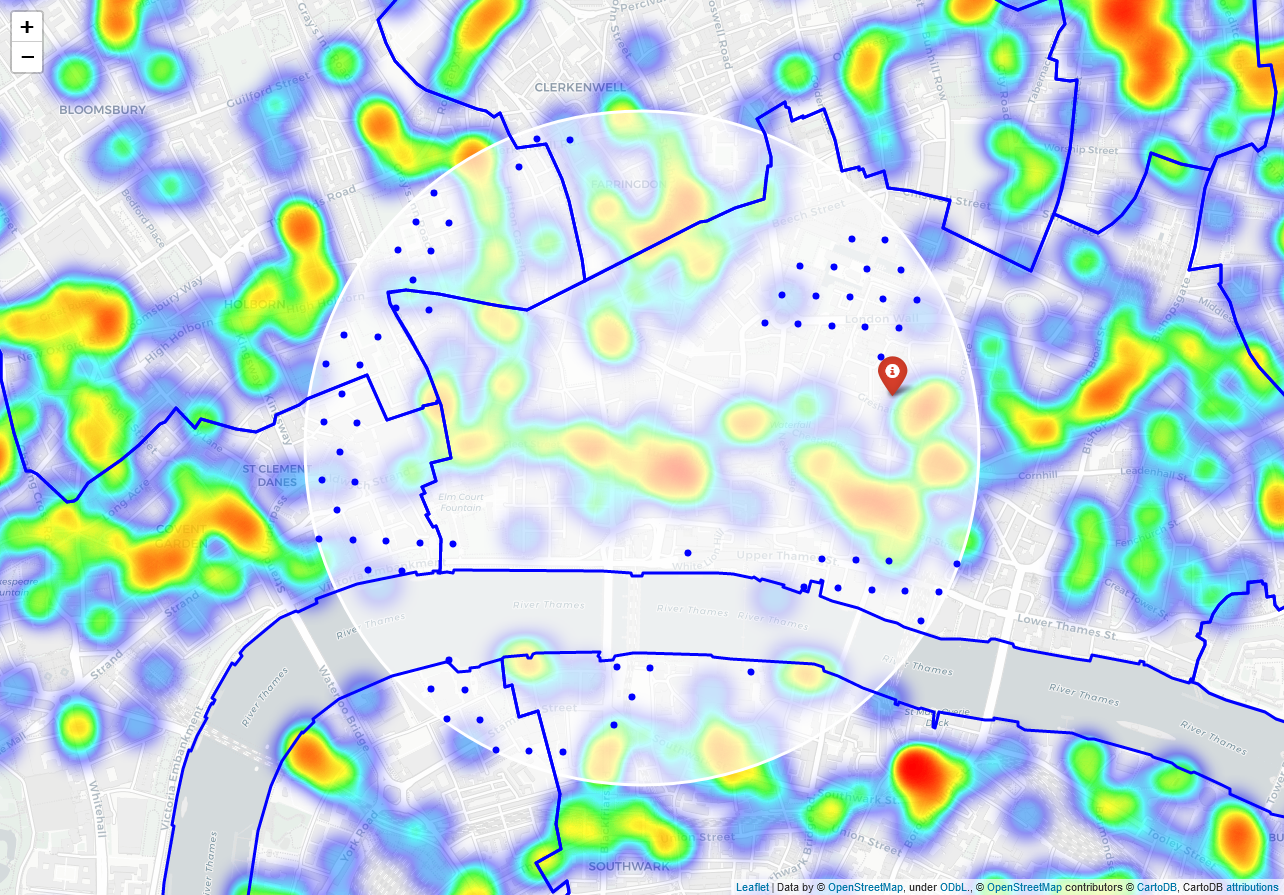
\includegraphics{15_best_loc_allrest}\end{center}

            % \begin{tcolorbox}[breakable, size=fbox, boxrule=.5pt, pad at break*=1mm, opacityfill=0]
% % \prompt{Out}{outcolor}{94}{\boxspacing}
% \begin{Verbatim}[commandchars=\\\{\}]
% <folium.folium.Map at 0x221ef9f93a0>
% \end{Verbatim}
% \end{tcolorbox}
        
    % \begin{tcolorbox}[breakable, size=fbox, boxrule=1pt, pad at break*=1mm,colback=cellbackground, colframe=cellborder]
% \prompt{In}{incolor}{95}{\boxspacing}
% \begin{Verbatim}[commandchars=\\\{\}]
% \PY{n}{save\PYZus{}map}\PY{p}{(}\PY{n}{map\PYZus{}best\PYZus{}loc}\PY{p}{,} \PY{l+s+s1}{\PYZsq{}}\PY{l+s+s1}{15\PYZus{}best\PYZus{}loc\PYZus{}allrest}\PY{l+s+s1}{\PYZsq{}}\PY{p}{)}
% \end{Verbatim}
% \end{tcolorbox}

    % \begin{Verbatim}[commandchars=\\\{\}]
% Map saved under '15\_best\_loc\_allrest.html' and '15\_best\_loc\_allrest.png'
    % \end{Verbatim}

    Looking good. We now have a bunch of locations fairly close to the
center of the city, and all of them respects our criterias.

Let's see that in the form of a \textbf{heatmap}:

    % \begin{tcolorbox}[breakable, size=fbox, boxrule=1pt, pad at break*=1mm,colback=cellbackground, colframe=cellborder]
% \prompt{In}{incolor}{96}{\boxspacing}
% \begin{Verbatim}[commandchars=\\\{\}]
% \PY{n}{best\PYZus{}locations} \PY{o}{=} \PY{p}{[}\PY{p}{[}\PY{n}{lat}\PY{p}{,} \PY{n}{lon}\PY{p}{]} \PY{k}{for} \PY{n}{lat}\PY{p}{,} \PY{n}{lon} \PY{o+ow}{in} \PY{n+nb}{zip}\PY{p}{(}\PY{n}{best\PYZus{}places}\PY{p}{[}\PY{l+s+s1}{\PYZsq{}}\PY{l+s+s1}{Latitude}\PY{l+s+s1}{\PYZsq{}}\PY{p}{]}\PY{p}{,} \PY{n}{best\PYZus{}places}\PY{p}{[}\PY{l+s+s1}{\PYZsq{}}\PY{l+s+s1}{Longitude}\PY{l+s+s1}{\PYZsq{}}\PY{p}{]}\PY{p}{)}\PY{p}{]}

% \PY{n}{map\PYZus{}best\PYZus{}loc\PYZus{}heat} \PY{o}{=} \PY{n}{folium}\PY{o}{.}\PY{n}{Map}\PY{p}{(}\PY{n}{location}\PY{o}{=}\PY{p}{[}\PY{n}{search\PYZus{}area\PYZus{}center\PYZus{}lat}\PY{p}{,} \PY{n}{search\PYZus{}area\PYZus{}center\PYZus{}long}\PY{p}{]}\PY{p}{,} \PY{n}{zoom\PYZus{}start}\PY{o}{=}\PY{l+m+mi}{15}\PY{p}{)}
% \PY{n}{HeatMap}\PY{p}{(}\PY{n}{best\PYZus{}locations}\PY{p}{,} \PY{n}{radius}\PY{o}{=}\PY{l+m+mi}{25}\PY{p}{)}\PY{o}{.}\PY{n}{add\PYZus{}to}\PY{p}{(}\PY{n}{map\PYZus{}best\PYZus{}loc\PYZus{}heat}\PY{p}{)}
% \PY{n}{folium}\PY{o}{.}\PY{n}{Marker}\PY{p}{(}\PY{p}{[}\PY{n}{city\PYZus{}latitude}\PY{p}{,} \PY{n}{city\PYZus{}longitude}\PY{p}{]}\PY{p}{,} \PY{n}{icon}\PY{o}{=}\PY{n}{folium}\PY{o}{.}\PY{n}{Icon}\PY{p}{(}\PY{n}{color}\PY{o}{=}\PY{l+s+s1}{\PYZsq{}}\PY{l+s+s1}{red}\PY{l+s+s1}{\PYZsq{}}\PY{p}{,} \PY{n}{icon}\PY{o}{=}\PY{l+s+s1}{\PYZsq{}}\PY{l+s+s1}{info\PYZhy{}sign}\PY{l+s+s1}{\PYZsq{}}\PY{p}{)}\PY{p}{,} \PY{n}{popup}\PY{o}{=}\PY{l+s+s1}{\PYZsq{}}\PY{l+s+s1}{City Center}\PY{l+s+s1}{\PYZsq{}}\PY{p}{)}\PY{o}{.}\PY{n}{add\PYZus{}to}\PY{p}{(}\PY{n}{map\PYZus{}best\PYZus{}loc\PYZus{}heat}\PY{p}{)}
% \PY{k}{for} \PY{n}{lat}\PY{p}{,} \PY{n}{lon} \PY{o+ow}{in} \PY{n+nb}{zip}\PY{p}{(}\PY{n}{best\PYZus{}places}\PY{p}{[}\PY{l+s+s1}{\PYZsq{}}\PY{l+s+s1}{Latitude}\PY{l+s+s1}{\PYZsq{}}\PY{p}{]}\PY{p}{,} \PY{n}{best\PYZus{}places}\PY{p}{[}\PY{l+s+s1}{\PYZsq{}}\PY{l+s+s1}{Longitude}\PY{l+s+s1}{\PYZsq{}}\PY{p}{]}\PY{p}{)}\PY{p}{:}
    % \PY{n}{folium}\PY{o}{.}\PY{n}{CircleMarker}\PY{p}{(}\PY{p}{[}\PY{n}{lat}\PY{p}{,} \PY{n}{lon}\PY{p}{]}\PY{p}{,} \PY{n}{radius}\PY{o}{=}\PY{l+m+mi}{2}\PY{p}{,} \PY{n}{color}\PY{o}{=}\PY{l+s+s1}{\PYZsq{}}\PY{l+s+s1}{blue}\PY{l+s+s1}{\PYZsq{}}\PY{p}{,} \PY{n}{fill}\PY{o}{=}\PY{k+kc}{True}\PY{p}{,} \PY{n}{fill\PYZus{}color}\PY{o}{=}\PY{l+s+s1}{\PYZsq{}}\PY{l+s+s1}{blue}\PY{l+s+s1}{\PYZsq{}}\PY{p}{,} \PY{n}{fill\PYZus{}opacity}\PY{o}{=}\PY{l+m+mi}{1}\PY{p}{)}\PY{o}{.}\PY{n}{add\PYZus{}to}\PY{p}{(}\PY{n}{map\PYZus{}best\PYZus{}loc\PYZus{}heat}\PY{p}{)} 
% \PY{n}{folium}\PY{o}{.}\PY{n}{GeoJson}\PY{p}{(}\PY{n}{london\PYZus{}boroughs\PYZus{}boundaries}\PY{p}{,} \PY{n}{style\PYZus{}function}\PY{o}{=}\PY{n}{boroughs\PYZus{}style}\PY{p}{,} \PY{n}{name}\PY{o}{=}\PY{l+s+s1}{\PYZsq{}}\PY{l+s+s1}{geojson}\PY{l+s+s1}{\PYZsq{}}\PY{p}{)}\PY{o}{.}\PY{n}{add\PYZus{}to}\PY{p}{(}\PY{n}{map\PYZus{}best\PYZus{}loc\PYZus{}heat}\PY{p}{)}
% \PY{n}{map\PYZus{}best\PYZus{}loc\PYZus{}heat}
% \end{Verbatim}
% \end{tcolorbox}

\begin{center}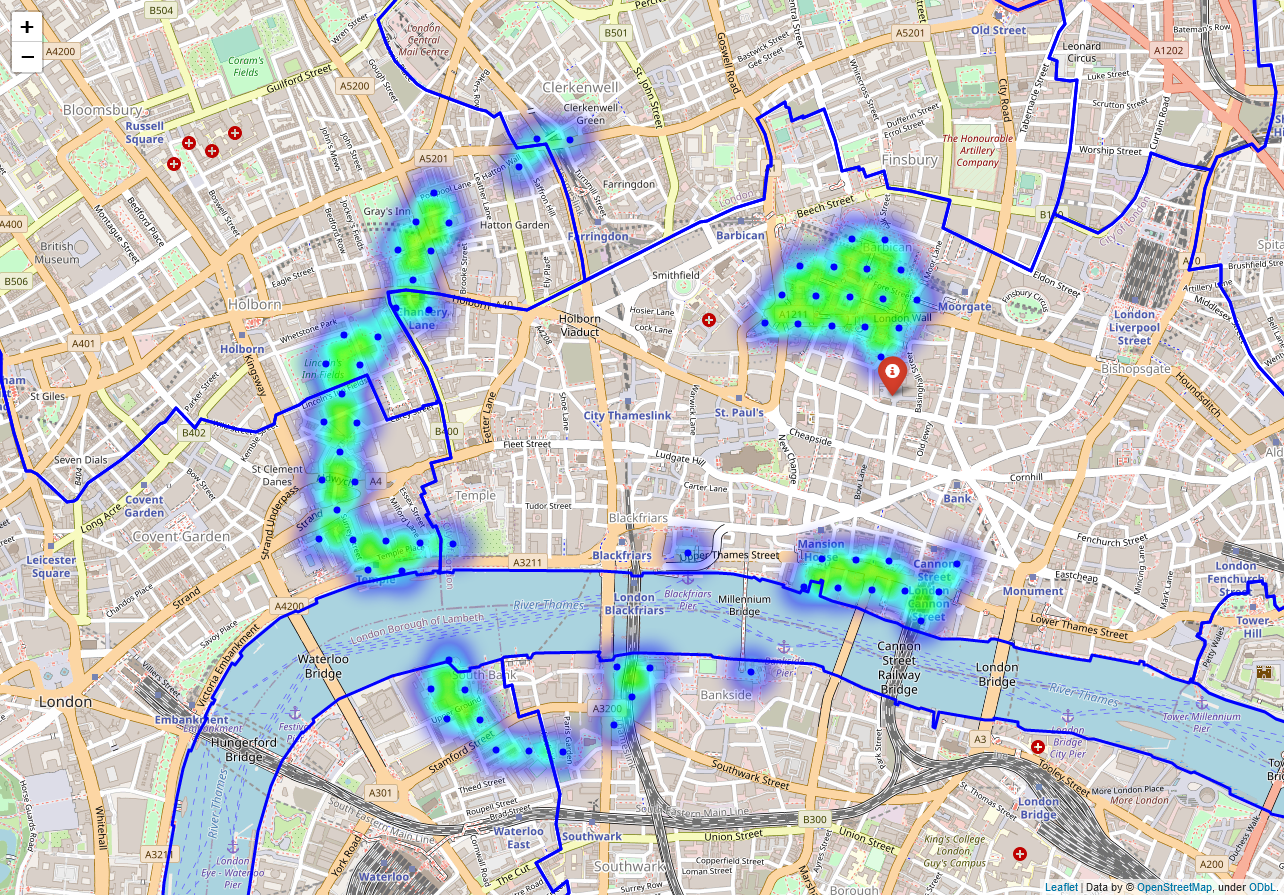
\includegraphics{16_best_loc_heat}\end{center}

            % \begin{tcolorbox}[breakable, size=fbox, boxrule=.5pt, pad at break*=1mm, opacityfill=0]
% % \prompt{Out}{outcolor}{96}{\boxspacing}
% \begin{Verbatim}[commandchars=\\\{\}]
% <folium.folium.Map at 0x221e720cc40>
% \end{Verbatim}
% \end{tcolorbox}
        
    % \begin{tcolorbox}[breakable, size=fbox, boxrule=1pt, pad at break*=1mm,colback=cellbackground, colframe=cellborder]
% \prompt{In}{incolor}{97}{\boxspacing}
% \begin{Verbatim}[commandchars=\\\{\}]
% \PY{n}{save\PYZus{}map}\PY{p}{(}\PY{n}{map\PYZus{}best\PYZus{}loc\PYZus{}heat}\PY{p}{,} \PY{l+s+s1}{\PYZsq{}}\PY{l+s+s1}{16\PYZus{}best\PYZus{}loc\PYZus{}heat}\PY{l+s+s1}{\PYZsq{}}\PY{p}{)}
% \end{Verbatim}
% \end{tcolorbox}

    % \begin{Verbatim}[commandchars=\\\{\}]
% Map saved under '16\_best\_loc\_heat.html' and '16\_best\_loc\_heat.png'
    % \end{Verbatim}

    We now have a clear indication of zones with low number of restaurants,
low number of \textbf{Italiant} restaurant nearby, and no
\textbf{French} ones close.

Let us now \textbf{cluster} those locations to create \textbf{centers of
zones containing good locations}. Those zones, their centers and
addresses will be the final result of our analysis.

    % \begin{tcolorbox}[breakable, size=fbox, boxrule=1pt, pad at break*=1mm,colback=cellbackground, colframe=cellborder]
% \prompt{In}{incolor}{98}{\boxspacing}
% \begin{Verbatim}[commandchars=\\\{\}]
% \PY{n}{number\PYZus{}of\PYZus{}clusters} \PY{o}{=} \PY{l+m+mi}{5}

% \PY{n}{best\PYZus{}xys} \PY{o}{=} \PY{n}{best\PYZus{}places}\PY{p}{[}\PY{p}{[}\PY{l+s+s1}{\PYZsq{}}\PY{l+s+s1}{X}\PY{l+s+s1}{\PYZsq{}}\PY{p}{,} \PY{l+s+s1}{\PYZsq{}}\PY{l+s+s1}{Y}\PY{l+s+s1}{\PYZsq{}}\PY{p}{]}\PY{p}{]}\PY{o}{.}\PY{n}{values}
% \PY{n}{kmeans} \PY{o}{=} \PY{n}{KMeans}\PY{p}{(}\PY{n}{n\PYZus{}clusters}\PY{o}{=}\PY{n}{number\PYZus{}of\PYZus{}clusters}\PY{p}{,} \PY{n}{random\PYZus{}state}\PY{o}{=}\PY{l+m+mi}{0}\PY{p}{)}\PY{o}{.}\PY{n}{fit}\PY{p}{(}\PY{n}{best\PYZus{}xys}\PY{p}{)}

% \PY{n}{cluster\PYZus{}centers} \PY{o}{=} \PY{p}{[}\PY{n}{xy\PYZus{}to\PYZus{}lonlat}\PY{p}{(}\PY{n}{cc}\PY{p}{[}\PY{l+m+mi}{0}\PY{p}{]}\PY{p}{,} \PY{n}{cc}\PY{p}{[}\PY{l+m+mi}{1}\PY{p}{]}\PY{p}{)} \PY{k}{for} \PY{n}{cc} \PY{o+ow}{in} \PY{n}{kmeans}\PY{o}{.}\PY{n}{cluster\PYZus{}centers\PYZus{}}\PY{p}{]}
% \end{Verbatim}
% \end{tcolorbox}

    % \begin{tcolorbox}[breakable, size=fbox, boxrule=1pt, pad at break*=1mm,colback=cellbackground, colframe=cellborder]
% \prompt{In}{incolor}{99}{\boxspacing}
% \begin{Verbatim}[commandchars=\\\{\}]
% \PY{n}{map\PYZus{}clusters\PYZus{}heat} \PY{o}{=} \PY{n}{folium}\PY{o}{.}\PY{n}{Map}\PY{p}{(}\PY{n}{location}\PY{o}{=}\PY{p}{[}\PY{n}{search\PYZus{}area\PYZus{}center\PYZus{}lat}\PY{p}{,} \PY{n}{search\PYZus{}area\PYZus{}center\PYZus{}long}\PY{p}{]}\PY{p}{,} \PY{n}{zoom\PYZus{}start}\PY{o}{=}\PY{l+m+mi}{15}\PY{p}{)}
% \PY{n}{folium}\PY{o}{.}\PY{n}{TileLayer}\PY{p}{(}\PY{l+s+s1}{\PYZsq{}}\PY{l+s+s1}{cartodbpositron}\PY{l+s+s1}{\PYZsq{}}\PY{p}{)}\PY{o}{.}\PY{n}{add\PYZus{}to}\PY{p}{(}\PY{n}{map\PYZus{}clusters\PYZus{}heat}\PY{p}{)}
% \PY{n}{HeatMap}\PY{p}{(}\PY{n}{restaurant\PYZus{}latlong}\PY{p}{)}\PY{o}{.}\PY{n}{add\PYZus{}to}\PY{p}{(}\PY{n}{map\PYZus{}clusters\PYZus{}heat}\PY{p}{)}
% \PY{n}{folium}\PY{o}{.}\PY{n}{Circle}\PY{p}{(}\PY{p}{[}\PY{n}{search\PYZus{}area\PYZus{}center\PYZus{}lat}\PY{p}{,} \PY{n}{search\PYZus{}area\PYZus{}center\PYZus{}long}\PY{p}{]}\PY{p}{,} \PY{n}{radius}\PY{o}{=}\PY{l+m+mi}{1000}\PY{p}{,} \PY{n}{color}\PY{o}{=}\PY{l+s+s1}{\PYZsq{}}\PY{l+s+s1}{white}\PY{l+s+s1}{\PYZsq{}}\PY{p}{,} \PY{n}{fill}\PY{o}{=}\PY{k+kc}{True}\PY{p}{,} \PY{n}{fill\PYZus{}opacity}\PY{o}{=}\PY{l+m+mf}{0.4}\PY{p}{)}\PY{o}{.}\PY{n}{add\PYZus{}to}\PY{p}{(}\PY{n}{map\PYZus{}clusters\PYZus{}heat}\PY{p}{)}
% \PY{n}{folium}\PY{o}{.}\PY{n}{Marker}\PY{p}{(}\PY{p}{[}\PY{n}{city\PYZus{}latitude}\PY{p}{,} \PY{n}{city\PYZus{}longitude}\PY{p}{]}\PY{p}{,} \PY{n}{icon}\PY{o}{=}\PY{n}{folium}\PY{o}{.}\PY{n}{Icon}\PY{p}{(}\PY{n}{color}\PY{o}{=}\PY{l+s+s1}{\PYZsq{}}\PY{l+s+s1}{red}\PY{l+s+s1}{\PYZsq{}}\PY{p}{,} \PY{n}{icon}\PY{o}{=}\PY{l+s+s1}{\PYZsq{}}\PY{l+s+s1}{info\PYZhy{}sign}\PY{l+s+s1}{\PYZsq{}}\PY{p}{)}\PY{p}{,} \PY{n}{popup}\PY{o}{=}\PY{l+s+s1}{\PYZsq{}}\PY{l+s+s1}{City Center}\PY{l+s+s1}{\PYZsq{}}\PY{p}{)}\PY{o}{.}\PY{n}{add\PYZus{}to}\PY{p}{(}\PY{n}{map\PYZus{}clusters\PYZus{}heat}\PY{p}{)}
% \PY{k}{for} \PY{n}{lon}\PY{p}{,} \PY{n}{lat} \PY{o+ow}{in} \PY{n}{cluster\PYZus{}centers}\PY{p}{:}
    % \PY{n}{folium}\PY{o}{.}\PY{n}{Circle}\PY{p}{(}\PY{p}{[}\PY{n}{lat}\PY{p}{,} \PY{n}{lon}\PY{p}{]}\PY{p}{,} \PY{n}{radius}\PY{o}{=}\PY{l+m+mi}{500}\PY{p}{,} \PY{n}{color}\PY{o}{=}\PY{l+s+s1}{\PYZsq{}}\PY{l+s+s1}{green}\PY{l+s+s1}{\PYZsq{}}\PY{p}{,} \PY{n}{fill}\PY{o}{=}\PY{k+kc}{True}\PY{p}{,} \PY{n}{fill\PYZus{}opacity}\PY{o}{=}\PY{l+m+mf}{0.25}\PY{p}{)}\PY{o}{.}\PY{n}{add\PYZus{}to}\PY{p}{(}\PY{n}{map\PYZus{}clusters\PYZus{}heat}\PY{p}{)} 
% \PY{k}{for} \PY{n}{lat}\PY{p}{,} \PY{n}{lon} \PY{o+ow}{in} \PY{n+nb}{zip}\PY{p}{(}\PY{n}{best\PYZus{}places}\PY{p}{[}\PY{l+s+s1}{\PYZsq{}}\PY{l+s+s1}{Latitude}\PY{l+s+s1}{\PYZsq{}}\PY{p}{]}\PY{p}{,} \PY{n}{best\PYZus{}places}\PY{p}{[}\PY{l+s+s1}{\PYZsq{}}\PY{l+s+s1}{Longitude}\PY{l+s+s1}{\PYZsq{}}\PY{p}{]}\PY{p}{)}\PY{p}{:}
    % \PY{n}{folium}\PY{o}{.}\PY{n}{CircleMarker}\PY{p}{(}\PY{p}{[}\PY{n}{lat}\PY{p}{,} \PY{n}{lon}\PY{p}{]}\PY{p}{,} \PY{n}{radius}\PY{o}{=}\PY{l+m+mi}{2}\PY{p}{,} \PY{n}{color}\PY{o}{=}\PY{l+s+s1}{\PYZsq{}}\PY{l+s+s1}{blue}\PY{l+s+s1}{\PYZsq{}}\PY{p}{,} \PY{n}{fill}\PY{o}{=}\PY{k+kc}{True}\PY{p}{,} \PY{n}{fill\PYZus{}color}\PY{o}{=}\PY{l+s+s1}{\PYZsq{}}\PY{l+s+s1}{blue}\PY{l+s+s1}{\PYZsq{}}\PY{p}{,} \PY{n}{fill\PYZus{}opacity}\PY{o}{=}\PY{l+m+mi}{1}\PY{p}{)}\PY{o}{.}\PY{n}{add\PYZus{}to}\PY{p}{(}\PY{n}{map\PYZus{}clusters\PYZus{}heat}\PY{p}{)}
% \PY{n}{folium}\PY{o}{.}\PY{n}{GeoJson}\PY{p}{(}\PY{n}{london\PYZus{}boroughs\PYZus{}boundaries}\PY{p}{,} \PY{n}{style\PYZus{}function}\PY{o}{=}\PY{n}{boroughs\PYZus{}style}\PY{p}{,} \PY{n}{name}\PY{o}{=}\PY{l+s+s1}{\PYZsq{}}\PY{l+s+s1}{geojson}\PY{l+s+s1}{\PYZsq{}}\PY{p}{)}\PY{o}{.}\PY{n}{add\PYZus{}to}\PY{p}{(}\PY{n}{map\PYZus{}clusters\PYZus{}heat}\PY{p}{)}
% \PY{n}{map\PYZus{}clusters\PYZus{}heat}
% \end{Verbatim}
% \end{tcolorbox}

\begin{center}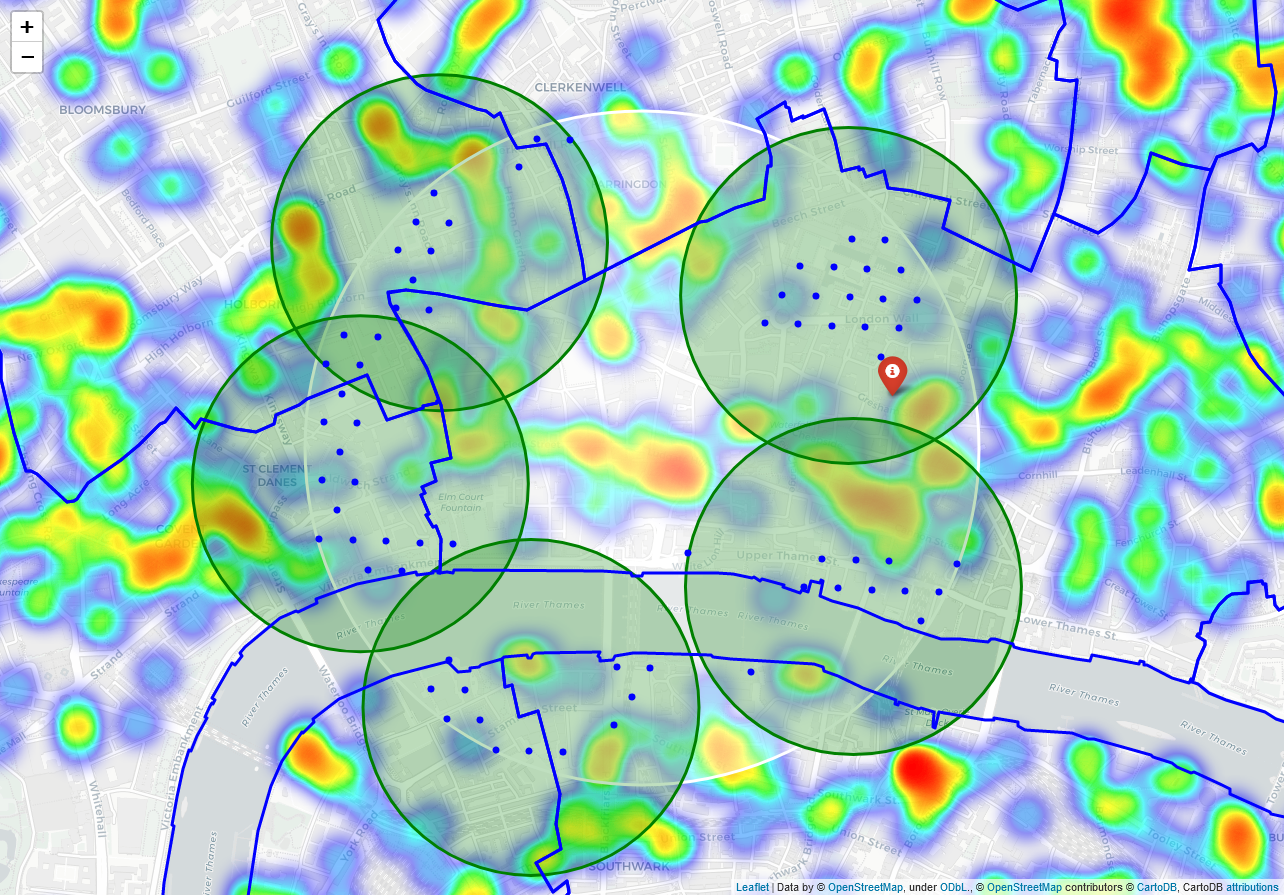
\includegraphics{17_clusters_heat}\end{center}

            % \begin{tcolorbox}[breakable, size=fbox, boxrule=.5pt, pad at break*=1mm, opacityfill=0]
% % \prompt{Out}{outcolor}{99}{\boxspacing}
% \begin{Verbatim}[commandchars=\\\{\}]
% <folium.folium.Map at 0x221efdcc700>
% \end{Verbatim}
% \end{tcolorbox}
        
    % \begin{tcolorbox}[breakable, size=fbox, boxrule=1pt, pad at break*=1mm,colback=cellbackground, colframe=cellborder]
% \prompt{In}{incolor}{100}{\boxspacing}
% \begin{Verbatim}[commandchars=\\\{\}]
% \PY{n}{save\PYZus{}map}\PY{p}{(}\PY{n}{map\PYZus{}clusters\PYZus{}heat}\PY{p}{,} \PY{l+s+s1}{\PYZsq{}}\PY{l+s+s1}{17\PYZus{}clusters\PYZus{}heat}\PY{l+s+s1}{\PYZsq{}}\PY{p}{)}
% \end{Verbatim}
% \end{tcolorbox}

    % \begin{Verbatim}[commandchars=\\\{\}]
% Map saved under '17\_clusters\_heat.html' and '17\_clusters\_heat.png'
    % \end{Verbatim}

    Our clusters groups most of the candidates locations, and their centers
are placed in the middle of the \textbf{hot} zones.

Let's see those zones on a city map without heatmap, using shaded areas
to indicate our clusters:

    % \begin{tcolorbox}[breakable, size=fbox, boxrule=1pt, pad at break*=1mm,colback=cellbackground, colframe=cellborder]
% \prompt{In}{incolor}{101}{\boxspacing}
% \begin{Verbatim}[commandchars=\\\{\}]
% \PY{n}{map\PYZus{}clusters} \PY{o}{=} \PY{n}{folium}\PY{o}{.}\PY{n}{Map}\PY{p}{(}\PY{n}{location}\PY{o}{=}\PY{p}{[}\PY{n}{search\PYZus{}area\PYZus{}center\PYZus{}lat}\PY{p}{,} \PY{n}{search\PYZus{}area\PYZus{}center\PYZus{}long}\PY{p}{]}\PY{p}{,} \PY{n}{zoom\PYZus{}start}\PY{o}{=}\PY{l+m+mi}{15}\PY{p}{)}
% \PY{n}{folium}\PY{o}{.}\PY{n}{Marker}\PY{p}{(}\PY{p}{[}\PY{n}{city\PYZus{}latitude}\PY{p}{,} \PY{n}{city\PYZus{}longitude}\PY{p}{]}\PY{p}{,} \PY{n}{icon}\PY{o}{=}\PY{n}{folium}\PY{o}{.}\PY{n}{Icon}\PY{p}{(}\PY{n}{color}\PY{o}{=}\PY{l+s+s1}{\PYZsq{}}\PY{l+s+s1}{red}\PY{l+s+s1}{\PYZsq{}}\PY{p}{,} \PY{n}{icon}\PY{o}{=}\PY{l+s+s1}{\PYZsq{}}\PY{l+s+s1}{info\PYZhy{}sign}\PY{l+s+s1}{\PYZsq{}}\PY{p}{)}\PY{p}{,} \PY{n}{popup}\PY{o}{=}\PY{l+s+s1}{\PYZsq{}}\PY{l+s+s1}{City Center}\PY{l+s+s1}{\PYZsq{}}\PY{p}{)}\PY{o}{.}\PY{n}{add\PYZus{}to}\PY{p}{(}\PY{n}{map\PYZus{}clusters}\PY{p}{)}
% \PY{k}{for} \PY{n}{lat}\PY{p}{,} \PY{n}{lon} \PY{o+ow}{in} \PY{n+nb}{zip}\PY{p}{(}\PY{n}{best\PYZus{}places}\PY{p}{[}\PY{l+s+s1}{\PYZsq{}}\PY{l+s+s1}{Latitude}\PY{l+s+s1}{\PYZsq{}}\PY{p}{]}\PY{p}{,} \PY{n}{best\PYZus{}places}\PY{p}{[}\PY{l+s+s1}{\PYZsq{}}\PY{l+s+s1}{Longitude}\PY{l+s+s1}{\PYZsq{}}\PY{p}{]}\PY{p}{)}\PY{p}{:}
    % \PY{n}{folium}\PY{o}{.}\PY{n}{Circle}\PY{p}{(}\PY{p}{[}\PY{n}{lat}\PY{p}{,} \PY{n}{lon}\PY{p}{]}\PY{p}{,} \PY{n}{radius}\PY{o}{=}\PY{l+m+mi}{250}\PY{p}{,} \PY{n}{color}\PY{o}{=}\PY{l+s+s1}{\PYZsq{}}\PY{l+s+s1}{\PYZsh{}00000000}\PY{l+s+s1}{\PYZsq{}}\PY{p}{,} \PY{n}{fill}\PY{o}{=}\PY{k+kc}{True}\PY{p}{,} \PY{n}{fill\PYZus{}color}\PY{o}{=}\PY{l+s+s1}{\PYZsq{}}\PY{l+s+s1}{\PYZsh{}0066ff}\PY{l+s+s1}{\PYZsq{}}\PY{p}{,} \PY{n}{fill\PYZus{}opacity}\PY{o}{=}\PY{l+m+mf}{0.07}\PY{p}{)}\PY{o}{.}\PY{n}{add\PYZus{}to}\PY{p}{(}\PY{n}{map\PYZus{}clusters}\PY{p}{)}
% \PY{k}{for} \PY{n}{lat}\PY{p}{,} \PY{n}{lon} \PY{o+ow}{in} \PY{n+nb}{zip}\PY{p}{(}\PY{n}{best\PYZus{}places}\PY{p}{[}\PY{l+s+s1}{\PYZsq{}}\PY{l+s+s1}{Latitude}\PY{l+s+s1}{\PYZsq{}}\PY{p}{]}\PY{p}{,} \PY{n}{best\PYZus{}places}\PY{p}{[}\PY{l+s+s1}{\PYZsq{}}\PY{l+s+s1}{Longitude}\PY{l+s+s1}{\PYZsq{}}\PY{p}{]}\PY{p}{)}\PY{p}{:}
    % \PY{n}{folium}\PY{o}{.}\PY{n}{CircleMarker}\PY{p}{(}\PY{p}{[}\PY{n}{lat}\PY{p}{,} \PY{n}{lon}\PY{p}{]}\PY{p}{,} \PY{n}{radius}\PY{o}{=}\PY{l+m+mi}{2}\PY{p}{,} \PY{n}{color}\PY{o}{=}\PY{l+s+s1}{\PYZsq{}}\PY{l+s+s1}{blue}\PY{l+s+s1}{\PYZsq{}}\PY{p}{,} \PY{n}{fill}\PY{o}{=}\PY{k+kc}{True}\PY{p}{,} \PY{n}{fill\PYZus{}color}\PY{o}{=}\PY{l+s+s1}{\PYZsq{}}\PY{l+s+s1}{blue}\PY{l+s+s1}{\PYZsq{}}\PY{p}{,} \PY{n}{fill\PYZus{}opacity}\PY{o}{=}\PY{l+m+mi}{1}\PY{p}{)}\PY{o}{.}\PY{n}{add\PYZus{}to}\PY{p}{(}\PY{n}{map\PYZus{}clusters}\PY{p}{)}
% \PY{k}{for} \PY{n}{lon}\PY{p}{,} \PY{n}{lat} \PY{o+ow}{in} \PY{n}{cluster\PYZus{}centers}\PY{p}{:}
    % \PY{n}{folium}\PY{o}{.}\PY{n}{Circle}\PY{p}{(}\PY{p}{[}\PY{n}{lat}\PY{p}{,} \PY{n}{lon}\PY{p}{]}\PY{p}{,} \PY{n}{radius}\PY{o}{=}\PY{l+m+mi}{500}\PY{p}{,} \PY{n}{color}\PY{o}{=}\PY{l+s+s1}{\PYZsq{}}\PY{l+s+s1}{green}\PY{l+s+s1}{\PYZsq{}}\PY{p}{,} \PY{n}{fill}\PY{o}{=}\PY{k+kc}{False}\PY{p}{)}\PY{o}{.}\PY{n}{add\PYZus{}to}\PY{p}{(}\PY{n}{map\PYZus{}clusters}\PY{p}{)} 
% \PY{n}{folium}\PY{o}{.}\PY{n}{GeoJson}\PY{p}{(}\PY{n}{london\PYZus{}boroughs\PYZus{}boundaries}\PY{p}{,} \PY{n}{style\PYZus{}function}\PY{o}{=}\PY{n}{boroughs\PYZus{}style}\PY{p}{,} \PY{n}{name}\PY{o}{=}\PY{l+s+s1}{\PYZsq{}}\PY{l+s+s1}{geojson}\PY{l+s+s1}{\PYZsq{}}\PY{p}{)}\PY{o}{.}\PY{n}{add\PYZus{}to}\PY{p}{(}\PY{n}{map\PYZus{}clusters}\PY{p}{)}
% \PY{n}{map\PYZus{}clusters}
% \end{Verbatim}
% \end{tcolorbox}

\begin{center}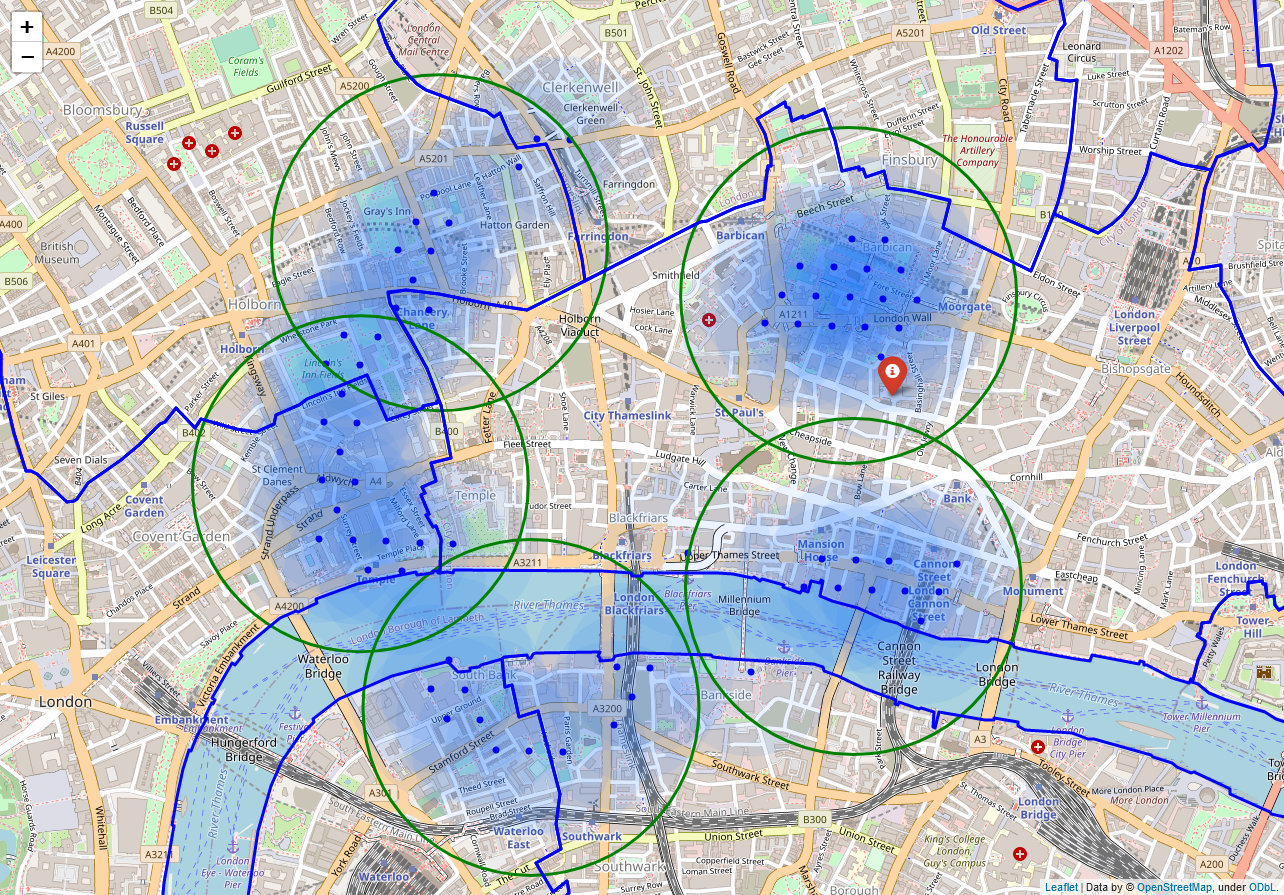
\includegraphics{18_clusters}\end{center}

            % \begin{tcolorbox}[breakable, size=fbox, boxrule=.5pt, pad at break*=1mm, opacityfill=0]
% % \prompt{Out}{outcolor}{101}{\boxspacing}
% \begin{Verbatim}[commandchars=\\\{\}]
% <folium.folium.Map at 0x221efe9b370>
% \end{Verbatim}
% \end{tcolorbox}
        
    % \begin{tcolorbox}[breakable, size=fbox, boxrule=1pt, pad at break*=1mm,colback=cellbackground, colframe=cellborder]
% \prompt{In}{incolor}{102}{\boxspacing}
% \begin{Verbatim}[commandchars=\\\{\}]
% \PY{n}{save\PYZus{}map}\PY{p}{(}\PY{n}{map\PYZus{}clusters}\PY{p}{,} \PY{l+s+s1}{\PYZsq{}}\PY{l+s+s1}{18\PYZus{}clusters}\PY{l+s+s1}{\PYZsq{}}\PY{p}{)}
% \end{Verbatim}
% \end{tcolorbox}

    % \begin{Verbatim}[commandchars=\\\{\}]
% Map saved under '18\_clusters.html' and '18\_clusters.png'
    % \end{Verbatim}

    Now it would be best to find the addresses of these clusters. Using the
same process as earlier before, let's reverse geocode them:

    % \begin{tcolorbox}[breakable, size=fbox, boxrule=1pt, pad at break*=1mm,colback=cellbackground, colframe=cellborder]
% \prompt{In}{incolor}{103}{\boxspacing}
% \begin{Verbatim}[commandchars=\\\{\}]
% \PY{n}{clusters\PYZus{}lst} \PY{o}{=} \PY{p}{[}\PY{p}{]}

% \PY{k}{for} \PY{n}{lon}\PY{p}{,} \PY{n}{lat} \PY{o+ow}{in} \PY{n}{cluster\PYZus{}centers}\PY{p}{:}
    % \PY{n}{x}\PY{p}{,} \PY{n}{y} \PY{o}{=} \PY{n}{lonlat\PYZus{}to\PYZus{}xy}\PY{p}{(}\PY{n}{lon}\PY{p}{,} \PY{n}{lat}\PY{p}{)}
    % \PY{n}{dist} \PY{o}{=} \PY{n}{calc\PYZus{}xy\PYZus{}distance}\PY{p}{(}\PY{n}{x}\PY{p}{,} \PY{n}{y}\PY{p}{,} \PY{n}{city\PYZus{}center\PYZus{}x}\PY{p}{,} \PY{n}{city\PYZus{}center\PYZus{}y}\PY{p}{)} \PY{o}{/} \PY{l+m+mi}{1000}
    % \PY{n}{tpl} \PY{o}{=} \PY{p}{(}\PY{n}{lat}\PY{p}{,} \PY{n}{lon}\PY{p}{,} \PY{n}{x}\PY{p}{,} \PY{n}{y}\PY{p}{,} \PY{n}{dist}\PY{p}{)}
    % \PY{n}{clusters\PYZus{}lst}\PY{o}{.}\PY{n}{append}\PY{p}{(}\PY{n}{tpl}\PY{p}{)}

% \PY{c+c1}{\PYZsh{} Dataframe}
% \PY{n}{cluster\PYZus{}data} \PY{o}{=} \PY{n}{pd}\PY{o}{.}\PY{n}{DataFrame}\PY{p}{(}\PY{n}{clusters\PYZus{}lst}\PY{p}{,} \PY{n}{columns}\PY{o}{=}\PY{p}{[}\PY{l+s+s1}{\PYZsq{}}\PY{l+s+s1}{Latitude}\PY{l+s+s1}{\PYZsq{}}\PY{p}{,}\PY{l+s+s1}{\PYZsq{}}\PY{l+s+s1}{Longitude}\PY{l+s+s1}{\PYZsq{}}\PY{p}{,}\PY{l+s+s1}{\PYZsq{}}\PY{l+s+s1}{X}\PY{l+s+s1}{\PYZsq{}}\PY{p}{,}\PY{l+s+s1}{\PYZsq{}}\PY{l+s+s1}{Y}\PY{l+s+s1}{\PYZsq{}}\PY{p}{,}\PY{l+s+s1}{\PYZsq{}}\PY{l+s+s1}{Distance from Center (km)}\PY{l+s+s1}{\PYZsq{}}\PY{p}{]}\PY{p}{)}
% \PY{n}{cluster\PYZus{}data}\PY{p}{[}\PY{l+s+s1}{\PYZsq{}}\PY{l+s+s1}{Address}\PY{l+s+s1}{\PYZsq{}}\PY{p}{]} \PY{o}{=} \PY{n}{cluster\PYZus{}data}\PY{o}{.}\PY{n}{apply}\PY{p}{(}\PY{k}{lambda} \PY{n}{x}\PY{p}{:} \PY{n}{get\PYZus{}address}\PY{p}{(}\PY{n}{x}\PY{p}{[}\PY{l+s+s1}{\PYZsq{}}\PY{l+s+s1}{Latitude}\PY{l+s+s1}{\PYZsq{}}\PY{p}{]}\PY{p}{,} \PY{n}{x}\PY{p}{[}\PY{l+s+s1}{\PYZsq{}}\PY{l+s+s1}{Longitude}\PY{l+s+s1}{\PYZsq{}}\PY{p}{]}\PY{p}{)}\PY{p}{,} \PY{n}{axis}\PY{o}{=}\PY{l+m+mi}{1}\PY{p}{)}
% \PY{n}{cluster\PYZus{}data} \PY{o}{=} \PY{n}{cluster\PYZus{}data}\PY{p}{[}\PY{p}{[}\PY{l+s+s1}{\PYZsq{}}\PY{l+s+s1}{Address}\PY{l+s+s1}{\PYZsq{}}\PY{p}{,}\PY{l+s+s1}{\PYZsq{}}\PY{l+s+s1}{Latitude}\PY{l+s+s1}{\PYZsq{}}\PY{p}{,}\PY{l+s+s1}{\PYZsq{}}\PY{l+s+s1}{Longitude}\PY{l+s+s1}{\PYZsq{}}\PY{p}{,}\PY{l+s+s1}{\PYZsq{}}\PY{l+s+s1}{Distance from Center (km)}\PY{l+s+s1}{\PYZsq{}}\PY{p}{,}\PY{l+s+s1}{\PYZsq{}}\PY{l+s+s1}{X}\PY{l+s+s1}{\PYZsq{}}\PY{p}{,}\PY{l+s+s1}{\PYZsq{}}\PY{l+s+s1}{Y}\PY{l+s+s1}{\PYZsq{}}\PY{p}{]}\PY{p}{]}

% \PY{c+c1}{\PYZsh{} Print}
% \PY{n}{cluster\PYZus{}data}
% \end{Verbatim}
% \end{tcolorbox}

\resizebox{\textwidth}{!}{%
    \begin{tabular}{llllll}
    Address &
    Latitude & Longitude &
    Distance from Center (km) & X & Y
    \\ \hline
    3, Brooke's Court, Gray's Inn, Holborn, London{\ldots} &
    51.519565 & -0.111601 &
    1.420752 & 700386.738823 & 5.711561e+06
    \\
    Monkwell Square, Barbican, City of London, Gre{\ldots} &
    51.518159 & -0.094044 &
    0.322339 & 701610.720723 & 5.711452e+06
    \\
    Hatfield House, 52, Stamford Street, Southwark{\ldots} &
    51.507155 & -0.107674 &
    1.420003 & 700713.661900 & 5.710192e+06
    \\
    Vintners Place, Upper Thames Street, Blackfria{\ldots} & 
    1.510383 & -0.093837 &
    0.580570 & 701659.495233 & 5.710589e+06
    \\
    Clement House, 97–99, Aldwych, St Clement Dane{\ldots} &
    51.513129 & -0.114999 &
    1.604640 & 700179.286900 & 5.710836e+06
    \end{tabular}
}

            % \begin{tcolorbox}[breakable, size=fbox, boxrule=.5pt, pad at break*=1mm, opacityfill=0]
% % \prompt{Out}{outcolor}{103}{\boxspacing}
% \begin{Verbatim}[commandchars=\\\{\}]
                                             % Address   Latitude  Longitude  \textbackslash{}
% 0  3, Brooke's Court, Gray's Inn, Holborn, London{\ldots}  51.519565  -0.111601
% 1  Monkwell Square, Barbican, City of London, Gre{\ldots}  51.518159  -0.094044
% 2  Hatfield House, 52, Stamford Street, Southwark{\ldots}  51.507155  -0.107674
% 3  Vintners Place, Upper Thames Street, Blackfria{\ldots}  51.510383  -0.093837
% 4  Clement House, 97–99, Aldwych, St Clement Dane{\ldots}  51.513129  -0.114999

   % Distance from Center (km)              X             Y
% 0                   1.420752  700386.738823  5.711561e+06
% 1                   0.322339  701610.720723  5.711452e+06
% 2                   1.420003  700713.661900  5.710192e+06
% 3                   0.580570  701659.495233  5.710589e+06
% 4                   1.604640  700179.286900  5.710836e+06
% \end{Verbatim}
% \end{tcolorbox}
        
    % We have created 5 addresses that locate clusters of \textbf{hot} zones.
% Theses zones represent locations with:
% \begin{itemize}
% \item
    % A low number of restaurants;
% \item
    % Few \textbf{Italian} restaurants;
% \item
    % No \textbf{French} restaurants.
% \end{itemize}

They are perfect to establish a new \textbf{French} restaurant.
Nevertheless, although zones are shown on map with a radius of 250
meters (in green), their shape is quite irregular and their
centers/addresses should be considered only as a starting point for
exploring area neighborhoods in search for potential restaurant
locations.

    % \begin{tcolorbox}[breakable, size=fbox, boxrule=1pt, pad at break*=1mm,colback=cellbackground, colframe=cellborder]
% \prompt{In}{incolor}{104}{\boxspacing}
% \begin{Verbatim}[commandchars=\\\{\}]
% \PY{n}{map\PYZus{}clusters\PYZus{}markers} \PY{o}{=} \PY{n}{folium}\PY{o}{.}\PY{n}{Map}\PY{p}{(}\PY{n}{location}\PY{o}{=}\PY{p}{[}\PY{n}{search\PYZus{}area\PYZus{}center\PYZus{}lat}\PY{p}{,} \PY{n}{search\PYZus{}area\PYZus{}center\PYZus{}long}\PY{p}{]}\PY{p}{,} \PY{n}{zoom\PYZus{}start}\PY{o}{=}\PY{l+m+mi}{15}\PY{p}{)}
% \PY{n}{folium}\PY{o}{.}\PY{n}{Marker}\PY{p}{(}\PY{n}{location}\PY{o}{=}\PY{p}{[}\PY{n}{city\PYZus{}latitude}\PY{p}{,} \PY{n}{city\PYZus{}longitude}\PY{p}{]}\PY{p}{,} \PY{n}{icon}\PY{o}{=}\PY{n}{folium}\PY{o}{.}\PY{n}{Icon}\PY{p}{(}\PY{n}{color}\PY{o}{=}\PY{l+s+s1}{\PYZsq{}}\PY{l+s+s1}{red}\PY{l+s+s1}{\PYZsq{}}\PY{p}{,} \PY{n}{icon}\PY{o}{=}\PY{l+s+s1}{\PYZsq{}}\PY{l+s+s1}{info\PYZhy{}sign}\PY{l+s+s1}{\PYZsq{}}\PY{p}{)}\PY{p}{,} \PY{n}{popup}\PY{o}{=}\PY{l+s+s1}{\PYZsq{}}\PY{l+s+s1}{City Center}\PY{l+s+s1}{\PYZsq{}}\PY{p}{)}\PY{o}{.}\PY{n}{add\PYZus{}to}\PY{p}{(}\PY{n}{map\PYZus{}clusters\PYZus{}markers}\PY{p}{)}
% \PY{k}{for} \PY{n}{lat}\PY{p}{,} \PY{n}{long}\PY{p}{,} \PY{n}{addr} \PY{o+ow}{in} \PY{n+nb}{zip}\PY{p}{(}\PY{n}{cluster\PYZus{}data}\PY{p}{[}\PY{l+s+s1}{\PYZsq{}}\PY{l+s+s1}{Latitude}\PY{l+s+s1}{\PYZsq{}}\PY{p}{]}\PY{p}{,} \PY{n}{cluster\PYZus{}data}\PY{p}{[}\PY{l+s+s1}{\PYZsq{}}\PY{l+s+s1}{Longitude}\PY{l+s+s1}{\PYZsq{}}\PY{p}{]}\PY{p}{,} \PY{n}{cluster\PYZus{}data}\PY{p}{[}\PY{l+s+s1}{\PYZsq{}}\PY{l+s+s1}{Address}\PY{l+s+s1}{\PYZsq{}}\PY{p}{]}\PY{p}{)}\PY{p}{:}
    % \PY{n}{folium}\PY{o}{.}\PY{n}{Marker}\PY{p}{(}\PY{p}{[}\PY{n}{lat}\PY{p}{,} \PY{n}{long}\PY{p}{]}\PY{p}{,} \PY{n}{popup}\PY{o}{=}\PY{n}{addr}\PY{p}{)}\PY{o}{.}\PY{n}{add\PYZus{}to}\PY{p}{(}\PY{n}{map\PYZus{}clusters\PYZus{}markers}\PY{p}{)}
% \PY{k}{for} \PY{n}{lat}\PY{p}{,} \PY{n}{long} \PY{o+ow}{in} \PY{n+nb}{zip}\PY{p}{(}\PY{n}{best\PYZus{}places}\PY{p}{[}\PY{l+s+s1}{\PYZsq{}}\PY{l+s+s1}{Latitude}\PY{l+s+s1}{\PYZsq{}}\PY{p}{]}\PY{p}{,} \PY{n}{best\PYZus{}places}\PY{p}{[}\PY{l+s+s1}{\PYZsq{}}\PY{l+s+s1}{Longitude}\PY{l+s+s1}{\PYZsq{}}\PY{p}{]}\PY{p}{)}\PY{p}{:}
    % \PY{n}{folium}\PY{o}{.}\PY{n}{Circle}\PY{p}{(}\PY{p}{[}\PY{n}{lat}\PY{p}{,} \PY{n}{long}\PY{p}{]}\PY{p}{,} \PY{n}{radius}\PY{o}{=}\PY{l+m+mi}{250}\PY{p}{,} \PY{n}{color}\PY{o}{=}\PY{l+s+s1}{\PYZsq{}}\PY{l+s+s1}{\PYZsh{}0000ff00}\PY{l+s+s1}{\PYZsq{}}\PY{p}{,} \PY{n}{fill}\PY{o}{=}\PY{k+kc}{True}\PY{p}{,} \PY{n}{fill\PYZus{}color}\PY{o}{=}\PY{l+s+s1}{\PYZsq{}}\PY{l+s+s1}{\PYZsh{}0066ff}\PY{l+s+s1}{\PYZsq{}}\PY{p}{,} \PY{n}{fill\PYZus{}opacity}\PY{o}{=}\PY{l+m+mf}{0.05}\PY{p}{)}\PY{o}{.}\PY{n}{add\PYZus{}to}\PY{p}{(}\PY{n}{map\PYZus{}clusters\PYZus{}markers}\PY{p}{)}
% \PY{n}{map\PYZus{}clusters\PYZus{}markers}
% \end{Verbatim}
% \end{tcolorbox}

\begin{center}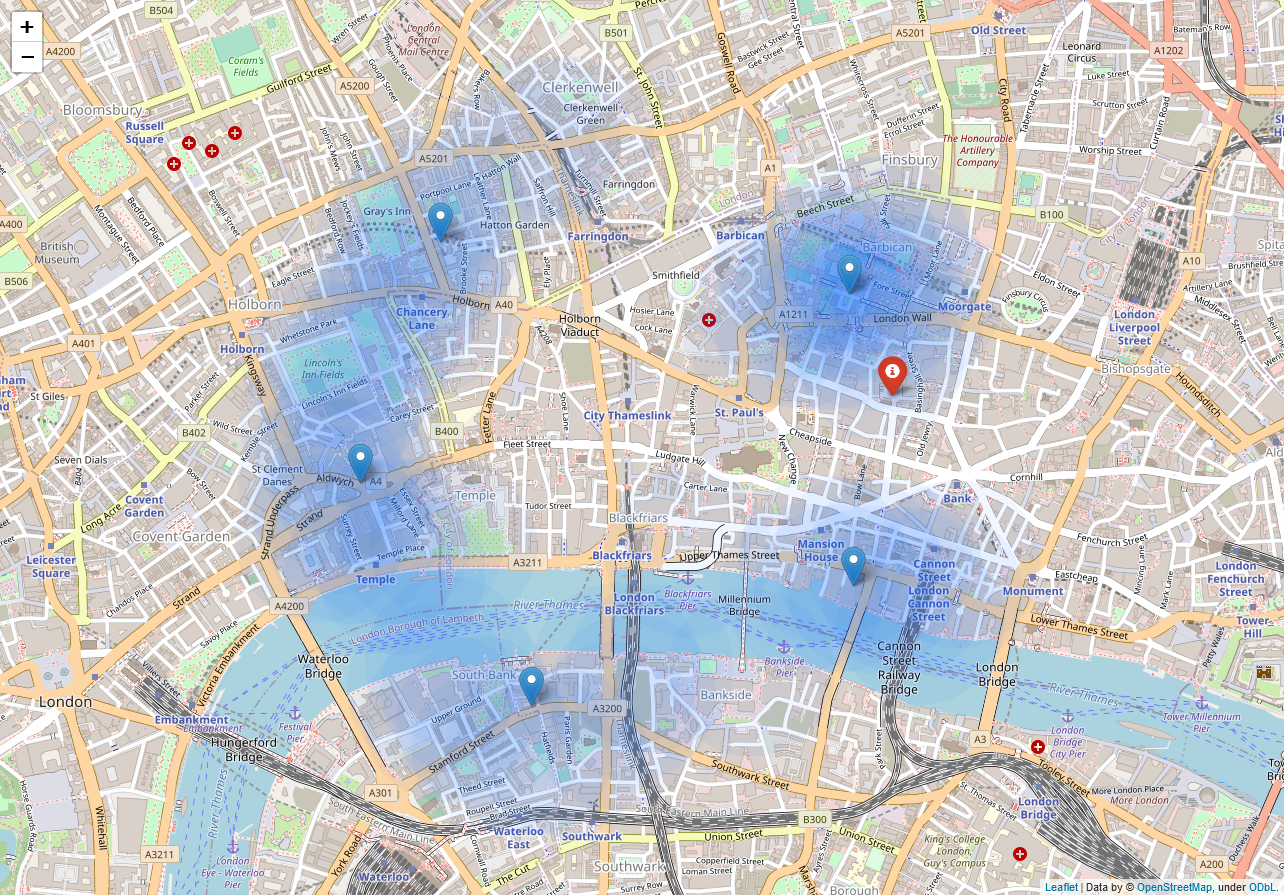
\includegraphics{19_clusters_markers}\end{center}

            % \begin{tcolorbox}[breakable, size=fbox, boxrule=.5pt, pad at break*=1mm, opacityfill=0]
% % \prompt{Out}{outcolor}{104}{\boxspacing}
% \begin{Verbatim}[commandchars=\\\{\}]
% <folium.folium.Map at 0x221f136bcd0>
% \end{Verbatim}
% \end{tcolorbox}
        
    % \begin{tcolorbox}[breakable, size=fbox, boxrule=1pt, pad at break*=1mm,colback=cellbackground, colframe=cellborder]
% \prompt{In}{incolor}{105}{\boxspacing}
% \begin{Verbatim}[commandchars=\\\{\}]
% \PY{n}{save\PYZus{}map}\PY{p}{(}\PY{n}{map\PYZus{}clusters\PYZus{}markers}\PY{p}{,} \PY{l+s+s1}{\PYZsq{}}\PY{l+s+s1}{19\PYZus{}clusters\PYZus{}markers}\PY{l+s+s1}{\PYZsq{}}\PY{p}{)}
% \end{Verbatim}
% \end{tcolorbox}

    % \begin{Verbatim}[commandchars=\\\{\}]
% Map saved under '19\_clusters\_markers.html' and '19\_clusters\_markers.png'
    % \end{Verbatim}

%    \begin{center}\rule{0.5\linewidth}{0.5pt}\end{center}

    \hypertarget{results-and-discussion}{%
\section{\texorpdfstring{Results and Discussion
}{Results and Discussion }}\label{results-and-discussion}}

London is a big city. So big that we first had to reduce our zone of
research to the City of London borough. And while the zone is already
pretty covered in restaurants (more thant 2.000 according to Foursquare,
for a 10x10km area), we can still see that the \textbf{French} cooking
isn't the most represented.

While we can find a high density of \textbf{French} restaurants in
Westminster, it clearly is not the case around the center. Considering
that the center is densely populated by other kitchen types, it is only
natural for us to to analysis this area in more details. And that is
what we have done.

After directing our attention to this more narrow area of interest,
which was 1x1km around Barbican, Blackfriars, and Temple, created a
dense grid of location candidates (spaced 100m appart, excluding the
River Thames); those locations were then filtered so that those with
more than two restaurants in radius of 250m, an \textbf{Italian}
restaurant close than 250m, or a \textbf{French} one close than 400m,
were excluded.

We then clustered these candidates into 5 zones of interest, and found
their respectives addresses.

It is important to note that this analysis is purely based on numbers.
There might be several good reasons for which theses places lacks
\textbf{French} restaurants, but without analysing the situation
\emph{by foot}, we can only suggest that they are, mathematically, the
best places to establish a new one.

%    \begin{center}\rule{0.5\linewidth}{0.5pt}\end{center}

    \hypertarget{conclusions}{%
\section{\texorpdfstring{Conclusions
}{Conclusions }}\label{conclusions}}

The goal of this project was to identify the best areas close to the
center of London, to establish either an \textbf{Italian}, or a
\textbf{French} restaurant. By calculating the restaurant densities, we
were able to advice a \textbf{French} one, as they are less prevalent,
suggest several locations that were lacking in density.

We used clusters in order to create major zones of interest, as it is
more relevant.

Obviously, the final decision will be made by the entrepreneur, and he
should also take into account other relevant information that we
couldn't analyse, such as:
\begin{itemize}
\item
    Proximity to offices;
\item
    Proximity to parks and / or water;
\item
    Noise levels;
\item
    Availability;
\item
    Rent prices;
\item
    \ldots{}
\end{itemize}

%    \begin{center}\rule{0.5\linewidth}{0.5pt}\end{center}

    \hypertarget{references}{%
\section{\texorpdfstring{References
}{References }}\label{references}}

\begin{itemize}
\tightlist
\item
  {[}1{]} \href{https://en.wikipedia.org/wiki/List_of_areas_of_London}{Wikipedia - Areas of London}
\item
  {[}2{]} \href{https://en.wikipedia.org/wiki/List_of_London_boroughs}{Wikipedia - London Boroughs}
\item
  {[}3{]} \href{https://skgrange.github.io/www/data/london_boroughs.json}{GeoJSON of London Boroughs}
\item
  {[}4{]} \href{https://jburnford.carto.com/tables/thames/public}{GeoJSON of the River Thames}
\item
  {[}5{]} \href{https://developer.foursquare.com/}{Foursquare API}
\end{itemize}


    % Add a bibliography block to the postdoc
    
    
    
\end{document}
